\documentclass[11pt, a4paper, french]{thloria}

% to be removed for final version
\ThesisDraft

\let\oldleftmark=\leftmark
\let\oldrightmark=\rightmark

\newcommand{\FaitMinitocs}{1} \newcommand{\CadresOvales}{1}
\newcommand{\FaitNomenclature}{1}

%%%%%%%%%%%%%%%%%%%%%%%%%%%%%%%%%%%%%%%%%%%%%%%%%%%%%%%%%
%%%% PACKAGES FONDAMENTAUX
%%%%%%%%%%%%%%%%%%%%%%%%%%%%%%%%%%%%%%%%%%%%%%%%%
\usepackage{ifthen}
\usepackage{ifpdf}


\usepackage[pdftex]{graphicx} % pour l'incusion de graphiques en pdf

\usepackage[intlimits]{amsmath} % amsmath, pour les maths
\usepackage{amssymb} % amssymb pour les symboles maths

%Pour pouvoir utiliser \allsectionsfont (utilis� dans le template)
\usepackage{sectsty}

% C'est quand m�me mieux, un pdf cliquable!
\usepackage[pdftex, colorlinks = true
%\usepackage[pdftex, colorlinks = false
   , pdfstartview = FitH 
   , linkcolor = blue
   , citecolor = blue
   , urlcolor = blue
   , bookmarksnumbered = true
   , bookmarksopen = true
   , pdfpagelabels
, pagebackref = true ]{tlhypref}


\usepackage{natbib} % citation of type (Dupont et al., 2013)
\renewcommand{\cite}{\citep}

\usepackage{morefloats} % accomodate large number of floats
\usepackage{placeins} 

\usepackage{fancybox} %pour encadrer les images en oval, shadow... Utilis� dans les macros

\usepackage{appendix} % pour annexes
\renewcommand\appendixname{Annexe}
\renewcommand\appendixpagename{Annexes}

%\usepackage{setspace} % pour singlespacing pour tabular



%%% Backref : permet de faire automatiquement des r�f�rences en arri�re cliquables dans la biblio, tr�s utile!
% setup the style of the backrefs from the bibliography %version ga�l compliqu�!
\RequirePackage[hyperpageref]{backref} % to be loaded after hyperref package
\newcommand{\backrefnotcitedstring}{\relax}%(Not cited.)
\newcommand{\backrefcitedsinglestring}[1]{(Page~#1.)}
\newcommand{\backrefcitedmultistring}[1]{(Pages~#1.)}
\renewcommand{\backreftwosep}{ et~} % seperate 2 pages
\renewcommand{\backreflastsep}{, et~} % seperate last of longer list
\renewcommand*{\backref}[1]{}  % Disable standard
\renewcommand*{\backrefalt}[4]{% Detailed backref
   \ifcase #1 %
   \backrefnotcitedstring%
   \or
   \backrefcitedsinglestring{#2}%
   \else
   \backrefcitedmultistring{#2}%
\fi}

% Si on veut des mini-tables des matieres :
\ifthenelse{\FaitMinitocs > 0}{
   \usepackage[french,nohints]{minitoc}%
   \mtcsetrules{minitoc}{off} % pour virer les lignes horizontales
   \mtcsettitle{minitoc}{} % pour virer le mot "<Sommaire"> au d�but des minitoc
   \setlength{\mtcindent}{0pt} % moins d'indentation � gauche des minitoc (d�faut 24pt)
   \mtcsetdepth{minitoc}{2} % pour voir sections et subsections.
}{}


%%%%%%%%%%%%%%%%%%%%%%%%%%%%%%%%%%%%%%%%%%%%%%%%%%%%%%%
% Pour pouvoir avoir des fleches depuis le texte vers des formules par exemple: TIKZ. Sert aussi pour l'index des notations, et pour les cadres
% http://www.fauskes.net/pgftikzexamples/global-nodes/
%%%%%%%%%%%%%%%%%%%%%%%%%%%%%%%%%%%%%%%%%%%%%%%%%%%%%%%
\usepackage{tikz,tkz-fct,tkz-2d}			% pour des supers graphiques trop cool, mieux que PSTricks.
\usetikzlibrary{snakes,arrows,shapes,backgrounds}
% For every picture that defines or uses external nodes, you'll have to apply the 'remember picture' style. To avoid some typing, we'll apply the style to all pictures.
\tikzstyle{every picture}+=[remember picture] 

% espace intelligent pour la fin d'une newcommand en tex (utilis� partout dans le fichier macro pour les maths)
\usepackage{xspace}

%gestion des unit�s !
\usepackage{sistyle}
%\SIstyle{German}   % Utile pour avoir une virgule avant les d�cimales et pas un point

% Les polices latex
\usepackage[latin1]{inputenc}
\usepackage[T1]{fontenc}
\usepackage{lmodern}
\usepackage[frenchb]{babel}

\usepackage[osf]{mathpazo}   % Palatino with smallcaps and oldstyle numbers
\usepackage[scaled]{helvet}  % Helvetica, scaled 95%


%Pour faire l'index des notations
\ifthenelse{\FaitNomenclature > 0}{
    \usepackage[norefpage,french,intoc]{nomencl}  %intoc rajoute une ligne dans la toc
    \renewcommand{\nomname}{\fontfamily{ppl}\selectfont Principales abbr�viations utilis�es} %Titre de la page
    \renewcommand{\pagedeclaration}[1]{~\dotfill\hyperpage{#1}}  %pour avoir des lignes de ... entre la description et le #page
    \renewcommand{\nomgroup}[1]{\bigskip}
    %\renewcommand{\nomgroup}[1]{%
    %\ifthenelse{\equal{#1}{A}}{\item[\textbf{\ChIntro}]}	  {
        %\ifthenelse{\equal{#1}{B}}{\medskip\item[\textbf{\ChMaxent}]}{
            %\ifthenelse{\equal{#1}{C}}{\medskip\item[\textbf{\ChImogene}]}{
                %\ifthenelse{\equal{#1}{D}}{\medskip\item[\textbf{\ChTrichomes}]}{
                    %\ifthenelse{\equal{#1}{E}}{\medskip\item[\textbf{\ChMuscle}]}{
                        %}}}}}
                    %}
                    %\def\ChCourantTitre{\ifcase\value{chapter} \or A\or B\or C \or D \or E\fi}
   %%%%%%%%%%%%%%%%%%%%%%%%%%%% D�finition de \ChCourantTitre ici!!!	


            \makenomenclature
         }{\newcommand{\nome}[2]{}}



% Pour ajouter des lignes comme biblio � la table des mati�res. Utilis� dans le template
         \usepackage[none]{tocbibind} 

%%%%%%%%%%%%%%%%%%%%%%%%%%%%%%%%%%%%%%%%%%%%%%%%%%%%%%%%%�
%%%% PACKAGES NON FONDAMENTAUX
%%%%%%%%%%%%%%%%%%%%%%%%%%%%%%%%%%%%%%%%%%%%%%%%%

%permet d'inclure des fichiers pdf directement dans le tex (articles en annexe), avec \includepdf[pages=-]{votre_fichier} 
         \usepackage{pdfpages}


         \usepackage{picins} %pour \parpic : images dans le texte � gauche ou � droite...

%http://www.cs.brown.edu/system/software/latex/doc/eqnarray.pdf
%Le fichier est � la racine du projet.
         \usepackage{equationarray}

% pour avoir les symboles \diameter, \frownie et \smiley
         \usepackage{wasysym}

% pour avoir les \ding{} : num�ros encercl�s
         \usepackage{pifont}

% pour des repr�sentation de vecteur sympa pour les physiciens
         \usepackage{vector}

% figures avec sous-figures et sous-captions:
         \usepackage[labelformat=empty, caption=true]{subfig}


\newcommand{\IncludePartOne}{1} 	\newcommand{\IncludePartTwo}{1}
\newcommand{\IncludePartThree}{1} \newcommand{\IncludePartFour}{1}

\newcommand{\IncludeAnnexes}{0} \newcommand{\IncludeAbstract}{1}

%\renewcommand{\baselinestretch}{1.5}




%%%%%%%%%%%%%%%%%%%%%%%%%%%%%%%%%%%%%%%%%%%%%%%%%%%%%%%%%%%%%%%%%%%%%%%%%%%%%%%%%%%%%%%%%%%%%%%%%%%%%%%%%%%%%%%%%%%%%%%%%%%%%%
%%%%%TOUT CE QUI CONCERNE TLORIA%%%%%%%%%%%%%%%%%%%%%%%%%%%%%%%%%%%%%%%%%%%%%%%%%%%%%%%%%%%%%%%%%%%%%
%%%%%%%%%%%%%%%%%%%%%%%%%%%%%%%%%%%%%%%%%%%%%%%%%%%%%%%%%%%%%%%%%%%%%%%%%%%%%%%%%%%%%%%%%%%%%%%%%%%%%%%%%%%%%%%%%%%%%%%%%%%%%%
%(cf _doc/TL-user.pdf pour plus de d�tails)
%-------------------------------------------------------------------
%                             En-tetes
%-------------------------------------------------------------------

% Les en-tetes: quelques exemples
%\UppercaseHeadings 
%\UnderlineHeadings
%\newcommand\bfheadings[1]{{\bf #1}}
%\FormatHeadingsWith{\bfheadings}
%\FormatHeadingsWith{\uppercase}
%\FormatHeadingsWith{\underline}
\newcommand\upun[1]{\uppercase{\underline{\underline{#1}}}}
\FormatHeadingsWith\upun

\newcommand\itheadings[1]{\textit{#1}}
\FormatHeadingsWith{\itheadings}

% pour avoir un trait sous l'en-tete:
\setlength{\HeadRuleWidth}{0.4pt}

%-------------------------------------------------------------------
%                         Les references
%-------------------------------------------------------------------

\NoChapterNumberInRef
\NoChapterPrefix

%-------------------------------------------------------------------
%                           Brouillons
%-------------------------------------------------------------------

% ceci ajoute une marque `brouillon' et la date
%\ThesisDraft



%%%%%%%%%%%%%%%%%%%%%%%%%%%%%%%%%%%%%%%%%%%%%%%%%%%%%%%%%%%%%%%%%%%%%%%%%%%%%%%%%%%%%%%%%%%%%%%%%%%%%%%%%%%%%%%%%%%%%%%%%%%%%%
%%%%%TOUT CE QUI NE CONCERNE PAS THLORIA%%%%%%%%%%%%%%%%%%%%%%%%%%%%%%%%%%%%%%%%%%%%%%%%%%%%%%%%%%%%%%%%%%%%%
%%%%%%%%%%%%%%%%%%%%%%%%%%%%%%%%%%%%%%%%%%%%%%%%%%%%%%%%%%%%%%%%%%%%%%%%%%%%%%%%%%%%%%%%%%%%%%%%%%%%%%%%%%%%%%%%%%%%%%%%%%%%%%

% Solution � la hache pour �viter les warning \oval et compagnie
\makeatletter
\renewcommand\@picture@warn{}
\makeatletter


% Un nouveau compteur pour les annexes
\newcounter{compteurannexes}
\renewcommand\thecompteurannexes{\Alph{compteurannexes}}


%%%% debut macro %%%% pour refaire les t�tes de chapitres
\makeatletter
\def\@makechapterhead#1{%
  %\vspace*{50\p@}% pour enlever l'espace avant le titre => minitoc rentre dans 1 page!
  \hrule
  \vspace*{10\p@}%
  {\parindent \z@ \raggedright \normalfont
    \ifnum \c@secnumdepth >\m@ne
      \if@mainmatter
        \huge{\fontfamily{ppl}\selectfont \bfseries \@chapapp\space \thechapter}
        \par\nobreak
          \vskip 10\p@
      \fi
    \fi
    \interlinepenalty\@M
    \Huge {\fontfamily{ppl}\selectfont #1}\par\nobreak
    \vspace*{10\p@}%
        \hrule
    \vskip 10\p@
}}
%%%%%Starred chapters (toc, lof, biblio)
\def\@schapter#1{\if@twocolumn
                   \@topnewpage[\@makeschapterhead{#1}]%
                 \else
                   \@makeschapterhead{#1}%
                   \@afterheading
                 \fi}
\def\@makeschapterhead#1{%
  \hrule
  \vspace*{10\p@}%
  {\parindent \z@ \raggedright \normalfont
    \interlinepenalty\@M
    \Huge{\fontfamily{ppl}\selectfont #1}
    \par\nobreak
    \vspace*{10\p@}%
        \hrule
    %\vskip 10\p@
  }}
\rmfamily
\makeatother
%%%% fin macro %%%%


% pour changer la police de toutes les sections
\allsectionsfont{\fontfamily{ppl}\selectfont}

% Num�rote les subsubsection pour pouvoir leur mettre un label et donc les voir appara�tre dans les minitocs
\setcounter{secnumdepth}{4}

% Mise en page des subsubsection avec un bullet, �crit en sffamily
\makeatletter
\renewcommand\subsubsection{\@startsection{subsubsection}{3}{10pt}%
                                     {-1.5ex \@plus -.2ex \@minus -.2ex}%
                                     {0.1ex \@plus.2ex}%
                                     {\sffamily\bf}}
\renewcommand\thesubsubsection{$\bullet$}          
\renewcommand*\l@subsubsection{\@dottedtocline{3}{7.0em}{1.5em}}                           
\makeatother              

% profondeur de la toc principale : 1 (minitoc : 2)
\setcounter{tocdepth}{1}


%%Pour avoir le titre du chapitre dans la liste des figures
%(xchapter est g�n�r� par minitoc)
\makeatletter
\let\l@xchapter\l@chapter
\makeatother

\begin{document}

%%%%%%%%%%%%%%%%%%%%%%%
%TITRE DES CHAPITRES
\newcommand{\ChIntro}{Introduction g�n�rale.}
\newcommand{\ChMaxent}{Mod�les de fixation des \TFs � l'ADN.}
\newcommand{\ChImogene}{{\em Imogene}: un algorithme d'identification de motifs et de modules de r�gulation transcriptionnelle}
\newcommand{\ChTrichomes}{�tude de la diff�renciation �pidermale chez la drosophile}
\newcommand{\ChMuscle}{�tude de la diff�renciation musculaire chez la souris}
\newcommand{\ChTest}{Chapitre d'exemples}


%%%%%%%%%%%%%%%%%%%%%%%%%%%%%%%%%%%%%%%%%%%%%%%%%%%%%%%%%%%%%%
%%%%%%%%% Le texte%%%%%%%%%%%%%%%%%%%%%%%%%%%
%%%%%%%%%%%%%%%%%%%%%%%%%%%%%%%%%%%%%%%%%%%%%%%%%%%%%%%%%%%%%%
\newcommand{\tf}{facteur de transcription\xspace}
\newcommand{\tfs}{facteurs de transcription\xspace}
\newcommand{\tfbs}{site de fixation de \tf\xspace}
\newcommand{\tfbss}{sites de fixation de \tf\xspace}
\newcommand{\tfbsss}{sites de fixation de \tfs\xspace}
\newcommand{\TF}{Facteur de Transcription\xspace}
\newcommand{\TFs}{Facteurs de Transcription\xspace}
\newcommand{\FT}{\TF}
\newcommand{\FTs}{\TFs}
\newcommand{\DI}{Information Directe\xspace}
\newcommand{\ID}{\DI}
\newcommand{\ft}{\tf}
\newcommand{\fts}{\tfs}
\newcommand{\TSS}{site de d�but de transcription}
\newcommand{\TSSs}{sites de d�but de transcription}
\newcommand{\CRM}{module de cis-r�gulation}
\newcommand{\CRMs}{modules de cis-r�gulation}

\newcommand{\apriori}{\textit{a priori}\xspace}
\newcommand{\aposteriori}{\textit{a posteriori}\xspace}
\newcommand{\cad}{c'est-�-dire\xspace}
\newcommand{\etal}{\textit{et al.}\xspace}

\newcommand{\denovo}{\textit{de novo}\xspace}
\newcommand{\via}{\textit{via}\xspace}
\newcommand{\insitu}{\textit{in situ}\xspace}
\newcommand{\invitro}{\textit{in vitro}\xspace}
\newcommand{\invivo}{\textit{in vivo}\xspace}
\newcommand{\chip}{ChIP\xspace}
\newcommand{\chipchip}{ChIP-on-chip\xspace}
\newcommand{\chipseq}{ChIP-seq\xspace}
\newcommand{\dmel}{\textit{Drosophila Melanogaster}\xspace}
\newcommand{\droso}{Drosophile\xspace}
\newcommand{\musmus}{\textit{Mus Musculus}\xspace}
\newcommand{\celegans}{\textit{Caenorhabditis Elegans}\xspace}
\newcommand{\ecoli}{\textit{Escherichia coli}\xspace}

\newcommand{\twi}{\textit{Twist}\xspace}
\newcommand{\myog}{\textit{Myog}\xspace}
\newcommand{\myod}{\textit{Myod1}\xspace}
\newcommand{\myf}{\textit{Myf5}\xspace}
\newcommand{\mrf}{\textit{Mrf4}\xspace}
\newcommand{\six}{\textit{Six}\xspace}
\newcommand{\six1}{\textit{Six1}\xspace}
\newcommand{\six14}{\textit{Six1,4}\xspace}
\newcommand{\six4}{\textit{Six4}\xspace}


%%%%%%%%%%%%%%%%%%%%%%%%%%%%%%%%%%%%%%%%%%%%%%%%%%%%%%%%%%%%%%
%%%%%%%%% Les maths%%%%%%%%%%%%%%%%%%%%%%%%%%%
%%%%%%%%%%%%%%%%%%%%%%%%%%%%%%%%%%%%%%%%%%%%%%%%%%%%%%%%%%%%%%
\newcommand{\pointformule}{\: .}
\newcommand{\virguleformule}{\: ,}
\newcommand{\finformule}{\vspace{-1cm}}

\newcommand{\OS}{\ensuremath{5^2 {\rm S}_{{1}/{2}}}\xspace}
\newcommand{\OPDD}{\ensuremath{5^2 {\rm P}_{{3}/{2}}}\xspace}
\newcommand{\OPDU}{\ensuremath{5^2 {\rm P}_{{1}/{2}}}\xspace}

\newcommand{\Etat}[1]{{| {#1} \rangle}}
\newcommand{\ket}[1]{\ensuremath{\left|#1\right\rangle}}
\newcommand{\bra}[1]{\left\langle #1\right|}


\newcommand{\Spin}[3]{\bra{#1} \widehat{S}_{#2} \ket{#3}}
\newcommand{\vr}{\ve{r}}
\newcommand{\rp}{\ve{r}^\prime}
\newcommand{\rpp}{\ve{r_\parallel}^{\prime\prime}}
\newcommand{\rA}{\ve{r_A}}
\newcommand{\uchap}{\widehat{u}}
\newcommand{\rrp}{(\ve{r},\rp)}
\newcommand{\rrpp}{(\ve{r},\rpp)}
\newcommand{\vu}{\ve{u}}

\newcommand{\FmF}[2]{{F=#1 , m_F=#2}\xspace}
\newcommand{\EtatFmF}[2]{\ensuremath{\Etat{ \FmF{#1}{#2} }}\xspace}
\newcommand{\EtatFprimemFprime}[2]{\ensuremath{\Etat{ F^\prime=#1 , m_F^\prime=#2 }}\xspace}
\newcommand{\EtatF}[1]{\ensuremath{\Etat{ F=#1 }}\xspace}
\newcommand{\EtatFprime}[1]{\ensuremath{\Etat{ F^\prime=#1 }}\xspace}
\newcommand{\mF}[1]{\ensuremath{\Etat{ m_F=#1 }}\xspace}
\newcommand{\mFprime}[1]{\ensuremath{\Etat{ m_{F^\prime}=#1 }}\xspace}
\newcommand{\mFv}[1]{\ensuremath{\Etat{ m_F }}\xspace}

\newcommand{\trdt}{\ensuremath{\EtatF{2} \to \EtatFprime{3}}\xspace}
\newcommand{\trud}{\ensuremath{\EtatF{1} \to \EtatFprime{2}}\xspace}


\newcommand{\keket}{\ensuremath{\left|\left|I=\frac32, m_I=\frac32; S=\frac12, m_s=\frac12 \right.\right\rangle}}
\newcommand{\kekett}{\ensuremath{\left|\left|I=\frac32, m_I=\frac32; S=\frac12, m_s=-\frac12 \right.\right\rangle}}
\newcommand{\kekettt}{\ensuremath{\left|\left|I=\frac32, m_I=\frac12; S=\frac12, m_s=\frac12 \right.\right\rangle}}
\newcommand{\kekk}{\EtatFmF{2}{2}}
\newcommand{\kek}{\EtatFmF{2}{1}}


\newcommand{\lambdaDB}{{\lambda_{\rm dB}}}

\newcommand{\mRb}{{m_{\rm Rb}}}
\newcommand{\Br}{{\ve{B\left( \ve{r} \right)}}}
\newcommand{\vectB}   {{\ve{B}}}
\newcommand{\vectBr}  {{\ve{B\left( \ve{r} \right)}}}
\newcommand{\vectBxyz}{{\ve{B\left( x,y,z \right)}}}
\newcommand{\modB}{{\Module{\vectB}}}
\newcommand{\modBr}{{\Module{\Br}}}

\newcommand{\omegaHF}{{\omega_{\rm hf}}}

\newcommand{\kb}{k_{\rm B}}
\newcommand{\muB}{\mu_{\rm B}}
\newcommand{\const}{{\mbox{const}}}

\newcommand{\Dix}[1]{\cdot 10^{#1}}

\newcommand{\Expo}[1]{\mathrm{e}^{\left(#1\right)}}

\newcommand{\ve}[1]{\overrightarrow{#1}}
\newcommand{\Module}[1]{\lvert #1 \rvert}

\newcommand{\Gradient}[1]{\ve{\nabla} \left( #1 \right) }
\newcommand{\Divergence}[1]{\ve{\nabla} \cdot #1 }

\newcommand{\rotr}{\ve{\nabla}_{\vr}}
\newcommand{\rotrp}{\ve{\nabla}_{\rp}}
\newcommand{\Erw}{\ve{E}(\vr,\om)}

\newcommand{\nonum}{\thispagestyle{empty}\addtocounter{page}{-1}}
\newcommand{\Ry}{Rydberg~}
\newcommand{\e}{\varepsilon}
\newcommand{\p}{\varphi}
\newcommand{\al}{\alpha}
\newcommand{\om}{\omega}
\newcommand{\de}{\delta}
\newcommand{\Om}{\Omega}
\newcommand{\ld}{\lambda}
\newcommand{\lV}{\lambda_V}
\newcommand{\lL}{\lambda_L}
\newcommand{\lac}{\lambda_{ac}}
\newcommand{\bsig}{{\boldsymbol\sigma}}
\newcommand{\si}{\sigma_i}
\newcommand{\sj}{\sigma_j}
\newcommand{\sh}{\sinh}
\newcommand{\ch}{\cosh}
\newcommand{\be}{\begin{equation}}
\newcommand{\ee}{\end{equation}}
\newcommand{\ds}{\displaystyle}
\newcommand{\bs}{\bigskip}


%\newcommand\numberthis{\addtocounter{equation}{1}\tag{\theequation}}
%\newcommand{\eq}[1]{\begin{equation}#1\end{equation*}}
%\newcommand{\eqn}[1]{\begin{equation}#1\end{equation}}
%\newcommand{\eqal}[1]{\begin{align*} #1 \end{align*}}
%\newcommand{\eqaln}[1]{\begin{align*} \numberthis#1 \end{align*}}
%\newcommand{\eqalacc}[1]{\[\left\{\begin{aligned}#1\end{aligned}\right.\]}
%\newcommand{\eqalaccn}[1]{\[\left\{\numberthis \begin{aligned}#1\end{aligned}\right.\]}

\newcommand{\Si}{\SI} % pr�vient les fautes de frappe!

\renewcommand{\tanh}{\mathrm{th}} % tangente hyperbolique
\renewcommand{\cosh}{\mathrm{ch}} % cosinus hyperbolique
\renewcommand{\sinh}{\mathrm{sh}} % sinus hyperbolique

\newcommand{\Bb}[3]{\ensuremath{\ve{B}_\text{biais}=(#1,#2,#3)}~G}

\newcommand{\omb}{\overline{\omega}}


\newcommand{\Vr}{\overrightarrow{r}}
\newcommand{\phir}{\phi(\Vr)}


\newcommand{\ReIm}[1]{\textup{#1}\,}
\renewcommand{\Re}{\ReIm{Re}}
\renewcommand{\Im}{\ReIm{Im}} 

\newcommand{\Gr}{\overleftrightarrow{G}}
\newcommand{\Gif}{\Gamma_{i\to f}}
\newcommand{\Gift}{\widetilde{\Gamma}_{i\to f}}
\newcommand{\Giftt}{\widetilde{\widetilde{\Gamma}}_{i\to f}}
\newcommand{\trif}{\ensuremath{\ket{i}\to\ket{f}}\xspace}

\newcommand{\pr}{^\prime}
\newcommand{\prpr}{^{\prime\prime}}



% Supprime de la version compil�e ce qu'il y a en argument : utile si on veut garder une trace de ce qui ne passe pas le barrage de la relecture!
\newcommand{\EnFaitNon}[1]{}

% Pour avoir des r�f�rences du style XX page YY
\newcommand{\FullRef}[1]{\ref{#1} page \pageref{#1}}
% Idem pour les �quations (rajoute des parenth�ses)
\newcommand{\FullEqRef}[1]{\eqref{#1} page \pageref{#1}}

% Pour rajouter un enlever localement une ligne � la page courante sans modifier tout le reste : tr�s utile pour la version finale
\newcommand{\AjouteLigne}{\enlargethispage{1\baselineskip}}
\newcommand{\RetireLigne}{\enlargethispage{-1\baselineskip}}

%%%%%%%%%%%%%%%%%%%%%%%%%%%%%%%%%%%%%%%%%%%%%%%%%%%%%%%
% TIKZ : Pour pouvoir avoir des supers jolies boites avec du texte et des formules exemple:
% http://www.fauskes.net/pgftikzexamples/boxes-with-text-and-math/
%%%%%%%%%%%%%%%%%%%%%%%%%%%%%%%%%%%%%%%%%%%%%%%%%%%%%%%
%%%%%%%%%%%%%%%%%%%%%%%%%%%%%%%%%%%%%%%%%%%%%%%%%%%%%%%
% Boite de D�finition
\tikzstyle{DefinitionBox}=[draw=black, fill=black!5, very thick, rectangle, rounded corners, inner sep=10pt, inner ysep=15pt]
\tikzstyle{DefinitionTitre}=[draw=black, rectangle, rounded corners, fill=white, text=black]
\newcommand{\Definition}[1]{%
\begin{center}\begin{tikzpicture}
\node [DefinitionBox] (box){%
	\begin{minipage}{0.92\textwidth}
		{\color{black}{#1}}
	\end{minipage}};
\node[DefinitionTitre, right=10pt] at (box.north west) {\sffamily D�finition\rmfamily};
\end{tikzpicture}\end{center}
}

%%%%%%%%%%%%%%%%%%%%%%%%%%%%%%%%%%%%%%%%%%%%%%%%%%%%%%%
% Boite de Notation
\tikzstyle{NotationBox}=[draw=black, fill=black!5, very thick, rectangle, rounded corners, inner sep=10pt, inner ysep=15pt]
\tikzstyle{NotationTitre}=[draw=black, rectangle, rounded corners, fill=white, text=black]
\newcommand{\Notation}[1]{%
\begin{center}\begin{tikzpicture}
\node [NotationBox] (box){%
	\begin{minipage}{0.92\textwidth}
		{\color{black}{#1}}
	\end{minipage}};
\node[NotationTitre, right=10pt] at (box.north west) {\sffamily Notation\rmfamily};
\end{tikzpicture}\end{center}
}

%%%%%%%%%%%%%%%%%%%%%%%%%%%%%%%%%%%%%%%%%%%%%%%%%%%%%%%
% Boite personnalisable
\tikzstyle{PersoBox}=[draw=black, fill=black!5, very thick, rectangle, rounded corners, inner sep=10pt, inner ysep=15pt]
\tikzstyle{PersoTitre}=[draw=black, rectangle, rounded corners, fill=white, text=black]
\newcommand{\Perso}[3]{%
\begin{figure}[!ht]
	\begin{center}\begin{tikzpicture}
	\node [PersoBox] (box){%
		\begin{minipage}{0.85\textwidth}
			{\color{black}{\small #3}}
		\end{minipage}};
	\refstepcounter{compteurencadres}\label{#2}
	\node[PersoTitre, right=10pt] at (box.north west) {\sffamily Encadr� \thecompteurencadres : #1\rmfamily};
	\end{tikzpicture}\end{center}
\end{figure}
}

%%%%%%%%%%%%%%%%%%%%%%%%%%%%%%%%%%%%%%%%%%%%%%%%%%%%%%%
% Boite de technique (un trait)
\tikzstyle{TechBox}=[draw=white, fill=black!1, rectangle, inner sep=5pt, inner ysep=10pt]
\tikzstyle{TechTitre}=[draw=black!1,  rectangle, fill=black!1, text=black]
\tikzstyle{TechLigne}=[color=black!30, line width=0.03cm, cap=round]
\newcommand{\Tech}[1]{%
\begin{center}\begin{tikzpicture}
\node [TechBox, below right,right=20pt] (box)
{%
    \begin{minipage}{0.85\textwidth}%
        {\color{black!85}{\footnotesize #1}}%
    \end{minipage}%
};
\node[TechTitre, right=0pt] at (box.north west) {\sffamily\small D�monstration\rmfamily};
\draw[TechLigne] (box.north west)--(box.south west);
\draw[TechLigne] (box.north west)++(0,-0.2)--++(1.9,0);
\end{tikzpicture}\end{center}}


%%%%%%%%%%%%%%%%%%%%%%%%%%%%%%%%%%%%%%%%%%%%%%%%%%%%%%%
% Boite d'Application num�rique
\tikzstyle{ApplicationNumeriqueBox}=[draw=green!80, fill=green!2, very thick, rectangle, rounded corners, inner sep=10pt, inner ysep=15pt]
\tikzstyle{ApplicationNumeriqueTitre}=[draw=green!80, rectangle, rounded corners, fill=white, text=black]
\newcommand{\AN}[1]{%
\begin{center}\begin{tikzpicture}
\node [ApplicationNumeriqueBox] (box){%
	\begin{minipage}{0.95\textwidth}
		{\color{black}{#1}}
	\end{minipage}};
\node[ApplicationNumeriqueTitre, right=10pt] at (box.north west) {\sffamily Application num�rique\rmfamily};
\end{tikzpicture}\end{center}
}

%%%%%%%%%%%%%%%%%%%%%%%%%%%%%%%%%%%%%%%%%%%%%%%%%%%%%%%
% Boite de Resultat important
\tikzstyle{ResultatBox}=[draw=red, fill=red!1, very thick, rectangle, rounded corners, inner sep=10pt, inner ysep=10pt]
\tikzstyle{ResultatTitre}=[draw=red, rectangle, rounded corners, fill=red, text=black]
\newcommand{\Resultat}[1]{%
\begin{center}\begin{tikzpicture}
\node [ResultatBox] (box){%
	\begin{minipage}{0.90\textwidth}
		{\color{black}{#1}\vskip-3mm}
	\end{minipage}};
%\node[ResultatTitre, right=10pt] at (box.north west) {R�sultat};
\end{tikzpicture}\end{center}
}

%%%%%%%%%%%%%%%%%%%%%%%%%%%%%%%%%%%%%%%%%%%%%%%%%%%%%%%
% Boite d'Interpr�tation
\tikzstyle{InterpretationBox}=[draw=blue, fill=blue!9, very thick,rectangle, rounded corners, inner sep=10pt, inner ysep=15pt]
\tikzstyle{InterpretationTitre}=[draw=blue, rectangle, rounded corners, fill=white, text=black]
\newcommand{\Interpretation}[1]{%
\begin{center}\begin{tikzpicture}\node [InterpretationBox] (box){%
	\begin{minipage}{0.95\textwidth}
		{\color{black}{#1}}
	\end{minipage}};
\node[InterpretationTitre, right=10pt] at (box.north west) {\sffamily Interpr�tation\rmfamily};
\end{tikzpicture}\end{center}}

%%%%%%%%%%%%%%%%%%%%%%%%%%%%%%%%%%%%%%%%%%%%%%%%%%%%%%%

%%%%%%%%%%%%%%%%%%%%%%%%%%%%%%%%%%%%%%%%%%%%%%%%%%%%%%%
% Boite de Remarque %%deux traits
\tikzstyle{RemarqueBox}=[fill=white, rectangle, inner sep=5pt, inner ysep=5pt]
\tikzstyle{RemarqueTitre}=[draw=white, thick, fill=white, text=black]
\tikzstyle{RemarqueLigne}=[color=black, line width=0.03cm, cap=round]
\newcommand{\Remarque}[1]{%
\begin{center}\begin{tikzpicture}
\node [RemarqueBox, below right] (box)
{%
    \begin{minipage}{0.85\textwidth}%
        {\color{black}{#1}}%
    \end{minipage}%
};
\node[RemarqueTitre, above right] at (box.north west) {\sffamily Remarque\rmfamily};
\draw[RemarqueLigne] (box.north west)++(0,0.6)--(box.south west);
\draw[RemarqueLigne] (box.north west)--++(2,0);
\draw (box.south west)++(-0.1,0)--(-0.1,0.6);
%\draw[very thick] (box.north east)--(box.south east);
\end{tikzpicture}\end{center}}

%%%%%%%%%%%%%%%%%%%%%%%%%%%%%%%%%%%%%%%%%%%%%%%%%%%%%%%
% Boite de Remarquee %%un trait, un titre, �crit petit
\tikzstyle{RemarqueeBox}=[fill=blue!2, rectangle, inner sep=5pt, inner ysep=5pt]
\tikzstyle{RemarqueeTitre}=[draw=white, thick, fill=white, text=black]
\tikzstyle{RemarqueeLigne}=[color=black, line width=0.03cm, cap=round]
\newcommand{\Remarquee}[2]{%
\begin{center}\begin{tikzpicture}
\node [RemarqueeBox, below right] (box)
{%
    \begin{minipage}{0.90\textwidth}%
        {\small \color{black}{#2}\normalsize}%
    \end{minipage}%
};
\node[RemarqueeTitre, above right] at (box.north west) {\sffamily Remarque~:~#1\rmfamily};
\draw[RemarqueeLigne] (box.north west)++(0,0.6)--(box.south west);
\draw[RemarqueeLigne] (box.north west)--++(2,0);
%\draw (box.south west)++(-0.1,0)--(-0.1,0.6);
%\draw[very thick] (box.north east)--(box.south east);
\end{tikzpicture}\end{center}}

%%%%%%%%%%%%%%%%%%%%%%%%%%%%%%%%%%%%%%%%%%%%%%%%%%%%%%%%%%%


%%%%%%%%%%%%%%%%%%%%%%%%%%%%%%%%%%%%%%%%%%%%%%%%%%%%%%%%%%%%%%
%%%%%%%%% Les figures%%%%%%%%%%%%%%%%%%%%%%%%%%%
%%%%%%%%%%%%%%%%%%%%%%%%%%%%%%%%%%%%%%%%%%%%%%%%%%%%%%%%%%%%%%
\newenvironment{fminipage}{%
\begin{Sbox}\begin{minipage}}
{%
\end{minipage}\end{Sbox}
\ifthenelse{\CadresOvales > 0}{\Ovalbox{\TheSbox}}{\TheSbox}
}

\newenvironment{cminipage}{%
\begin{Sbox}\begin{minipage}}
{%
\end{minipage}\end{Sbox}
\ifthenelse{\CadresOvales > 0}{\shadowbox{\TheSbox}}{\TheSbox}
}

\newcommand{\MinipageWidth}{15cm}
\newcommand{\CaptionWidth}{14.6cm}
\newcommand{\CaptionMargin}{0.4cm}
\newcommand{\FigWidth}{14.5cm}
\newcommand{\CaptionFig}[1]{\caption{\small{#1}}}
\newcommand{\CaptionTocCaptionFig}[2]{\caption[#1]{\small{#2}}}
\newcommand{\captionbf}[2]{\caption[#1]{\small \textbf{#1.}{#2}}}

% Les figures ombr�es *********************************************
\newenvironment{GaelFigureSh}[1][\MinipageWidth]{%
\begin{figure}[!ht]
\centering
\begin{cminipage}{#1}
\centering
\vspace{\CaptionMargin}
\pgfmathqparse{#1-\CaptionMargin-\CaptionMargin}
\begin{minipage}{\pgfmathresult pt}
\centering
}{%
\end{minipage}
\end{cminipage}
\end{figure}}
\newcommand{\bfigsh}{\begin{GaelFigureSh}}
\newcommand{\efigsh}{\end{GaelFigureSh}}

% Les figures normales *********************************************
\newenvironment{GaelFigure}[1][\MinipageWidth]{%
\begin{figure}[!ht]
\centering
\begin{fminipage}{#1}
\centering
\vspace{\CaptionMargin}
\pgfmathqparse{#1-\CaptionMargin-\CaptionMargin}
\begin{minipage}{\pgfmathresult pt}
\centering
}{%
\end{minipage}
\end{fminipage}
\end{figure}}
\newcommand{\bfig}{\begin{GaelFigure}}
\newcommand{\efig}{\end{GaelFigure}}

% Les figures : pleine page ***************************************
\newenvironment{GaelFigurep}[1][\MinipageWidth]{%
\begin{figure}[!htbp]
\centering
\begin{fminipage}{#1}
\centering
\vspace{\CaptionMargin}
\pgfmathqparse{#1-\CaptionMargin-\CaptionMargin}
\begin{minipage}{\pgfmathresult pt}
\centering
}{%
\end{minipage}
\end{fminipage}
\end{figure}}
\newcommand{\bfigp}{\begin{GaelFigurep}}
\newcommand{\efigp}{\end{GaelFigurep}}


%%%%%%%%%%%%%%%%%%%%%%%%%%%%%%%%%%%%%%%%%%%%%%%%%%%%%%%%%%%%%%
%%%%%%%%% Les tableaux%%%%%%%%%%%%%%%%%%%%%%%%%%%
%%%%%%%%%%%%%%%%%%%%%%%%%%%%%%%%%%%%%%%%%%%%%%%%%%%%%%%%%%%%%%
\newenvironment{CedTableau}[1][\MinipageWidth]{%
\begin{table}[!ht]
\centering
\begin{fminipage}{#1}
\centering
\vspace{\CaptionMargin}
\pgfmathqparse{#1-\CaptionMargin-\CaptionMargin}
\begin{minipage}{\pgfmathresult pt}
\centering
}{%
\end{minipage}
\end{fminipage}
\end{table}}
\newcommand{\btab}{\begin{CedTableau}}
\newcommand{\etab}{\end{CedTableau}}


%%%%%%%%%%%%%%%%%%%%%%%%%%%%%%%%%%%%%%%%%%%%%%%%%%%%
%% Pour faire des supers fleches d'highlight entre texte et �quation %%
%% http://www.fauskes.net/pgftikzexamples/global-nodes/
%% On d�finit un bout de fleche, et un d�part de fleche, puis on dit de faire les fleches....

\newcommand{\DepartHighlightColorNoTexte}[1]{ \tikz\node[fill=#1!20,draw, circle](From#1){};}

\newcommand{\DepartHighlightColor}[2]{ \tikz[baseline=(From#1.base)] {\node[fill=#1!20](From#1){#2};}}

\newcommand{\ArriveeHiglightColor}[2]{
\tikz[baseline=(To#1.base)] {\node[fill=#1!20](To#1){#2};}}

\newcommand{\MakeFlecheHighlightColor}[1]{ \begin{tikzpicture}
[overlay]\path[->](From#1)edge%[bend left]
(To#1);
\end{tikzpicture}}


%%%%%%%%%%%%%%%%%%%%%%%%%%%%%%%%%%%%%%%%%%%%%%%%%%%%%%%%%%%%%%
%%%%%%%%% Les listes%%%%%%%%%%%%%%%%%%%%%%%%%%%
%%%%%%%%%%%%%%%%%%%%%%%%%%%%%%%%%%%%%%%%%%%%%%%%%%%%%%%%%%%%%%
%check tick : \surd
%fl�che droite creuse : \triangleright
%rond : bullet 	
%%%REFERENCE : http://www.artofproblemsolving.com/LaTeX/AoPS_L_GuideSym.php


\newenvironment{maliste}[1]%
{ \begin{list}%
	{$\triangleright$}%
	{\setlength{\labelwidth}{10pt}%
	 \setlength{\leftmargin}{#1pt}%
	 %\setlength{\itemsep}{\parsep}
	\setlength{\itemsep}{0pt}
}}%
{ \end{list} }

\newenvironment{malistee}[1]%
{ \begin{list}%
	{$\to$}%
	{\setlength{\labelwidth}{0pt}%
	 \setlength{\leftmargin}{#1pt}%
	 %\setlength{\itemsep}{\parsep}
	\setlength{\itemsep}{0pt}
}}%
{ \end{list} }

\newenvironment{malistebullet}[1]%
{ \begin{list}%
	{$\bullet$\refstepcounter{subsubsection}}%
	{\setlength{\labelwidth}{0pt}%
	 \setlength{\leftmargin}{#1pt}%
	 %\setlength{\itemsep}{\parsep}
	%\setlength{\itemsep}{0pt}
}}%
{ \end{list} }

\newcommand{\blst}[1]{\begin{maliste}{#1}}
\newcommand{\elst}{\end{maliste}}
\newcommand{\blste}[1]{\begin{malistee}{#1}}
\newcommand{\elste}{\end{malistee}}
\newcommand{\blstbul}[1]{\begin{malistebullet}{#1}}
\newcommand{\elstbul}{\end{malistebullet}}

%%Liste personnalisable
\newenvironment{malisteperso}[2]%
{ \begin{list}%
	{$#2$}%
	{\setlength{\labelwidth}{10pt}%
	 \setlength{\leftmargin}{#1pt}%
	 %\setlength{\itemsep}{\parsep}
	\setlength{\itemsep}{0pt}
}}%
{ \end{list} }


%%%%%%%%%%%%%%%%%%%%%%%%%%%%%%%%%%%%%%%%%%%%%%%%%%%%%%%%%%%%%%
%%%%%%%%% Les annexes (c'est crad de mettre �a l� mais bon!) %
%%%%%%%%%%%%%%%%%%%%%%%%%%%%%%%%%%%%%%%%%%%%%%%%%%%%%%%%%%%%%%

\newcommand{\AnnexTitreCed}[4]
{
%\pagestyle{plain}
\renewcommand{\leftmark}{Annexe #1 - #2}
\renewcommand{\rightmark}{Annexe #1 - #2}
 %\hrule
  \vspace{15pt}%
  {\Huge \fontfamily{ppl}\selectfont \textbf{Annexe #1}}
   \par\nobreak
    \vspace{20pt}
   {\Huge \fontfamily{ppl}\selectfont #2}
    \vspace{10pt}
       \hrule
   \vskip20pt
	\refstepcounter{compteurannexes}\label{#3}
  \normalsize
  #4
  \EmptyNewPage
}


\newcommand{\Article}[1]
{
%\pagestyle{plain}
\renewcommand{\leftmark}{Article}
\renewcommand{\rightmark}{Article}
 \hrule
  \vspace{15pt}%
   {\Huge \fontfamily{ppl}\selectfont Article}
    \vspace{10pt}
       \hrule
   \vskip20pt
  \normalsize
  #1
  \EmptyNewPage
}



%%%%%%%%%%%%%%%%%%%%%%%%%%%%%%%%%%%%%%%%%%%%%%%%%%%%%%%%%%%%%%
%%%%%%%%% Pour la liste des notations %%%%%%%%%%%%%%%%%%%%%
%%%%%%%%%%%%%%%%%%%%%%%%%%%%%%%%%%%%%%%%%%%%%%%%%%%%%%%%%%%%%%


	% ************************************************************************
		% Pour fair une note dans la marge !
		% Command for inserting a todo item
		\definecolor{orange}{rgb}{1,0.5,0}
		\tikzstyle{notestyleright} = [right, draw=black, fill=blue!1]%, text width = 1cm]
		\tikzstyle{notestyleleft} = [notestyleright, left]
		\tikzstyle{connectstyle} = [draw = orange, thick]
		\newcommand{\todo}[1]{%
		% Add to todo list
		%\addcontentsline{tdo}{todo}{\protect{#1}}%
		%
		\begin{tikzpicture}[remember picture]%, baseline=7.5ex]%
		  \node [coordinate] (inText) {};
		\end{tikzpicture}%
		%
		% Make the margin par
		\marginpar[%
		{% Draw note in left margin
		 \tikz[remember picture] \path (0,0)++(1.8,0)++(-0.2,0)node[notestyleleft] (inNote) {\hyperlink{nomenclaturepage}{#1}};}%
		]{% Draw note in right margin
		  \tikz[remember picture] \path (0,0)++(0.2,0)node[notestyleright] (inNote) {\hyperlink{nomenclaturepage}{#1}};%
		}
		}

 %\ChCourantTitre est d�fini dans le fichier packages...
	\newcommand{\nome}[2]{%
      \nomenclature[\ChCourantTitre]{#1}{#2}%
      \todo{#1}%  ---------------------------------------la commande todo{truc} fout le truc dans la marge du bon cot�
  }


%%%%%%%%%%%%%%%%%%%%%%%%%%%%%%%%%%%%%%%%%%%%%%%%%%%%%%%%%%%%%%%%%%%%%%%%%%%%%%%%%%%%%%%%%%%%%%%%%%%%%%%%%%%%%%%%%%%%%%%%%%%%%%
%%%%%%%%%%%%%%%%%%%%%%%%%%%%%%%%%%%%%%%%%%%%%%%%%%%%%%%%%%%%%%%%%%%%%%%%%%%%%%%%%%%%%%%%%%%%%%%%%%%%%%%%%%%%%%%%%%%%%%%%%%%%%%
%%%%%%%%%%%%%%%%%%%%%%%%%%%%%%%%%%%%%%%%%%%%%%%%%%%%%%%%%%%%%%%%%%%%%%%%%%%%%%%%%%%%%%%%%%%%%%%%%%%%%%%%%%%%%%%%%%%%%%%%%%%%%%

      \OddHead={{\leftmark\rightmark}{\hfil\slshape\rightmark}}
      \EvenHead={{\leftmark}{{\slshape\leftmark}\hfil}}
      \OddFoot={\hfil\thepage}
      \EvenFoot={\thepage\hfil}
      \pagestyle{ThesisHeadingsII}
      
      %\ChapterPageStyle{ThesisHeadingsII}
      %\PartPageStyle{ThesisHeadingsII}

%-------------------------------------------------------------------
%                          Encadrements
%-------------------------------------------------------------------

% encadre les chapitres dans la table des matieres:
% (ces commandes doivent figurer apres \begin{document}
%\FrameChaptersInToc  
%\FramePartsInToc


%-------------------------------------------------------------------
%            Reinitialisation de la numerotation des chapitres
%-------------------------------------------------------------------
% Si la commande suivante est presente,
% elle doit figurer APRES \begin{document}
% et avant la premiere commande \part
%\ResetChaptersAtParts 

%-------------------------------------------------------------------
%               mini-tables des matieres par chapitre
%-------------------------------------------------------------------
% preparer les mini-tables des matieres par chapitre.
% (commande de minitoc.sty)
\ifthenelse{\FaitMinitocs > 0}{\dominitoc}{}


%-------------------------------------------------------------------
%                  ecriture de `Chapitre'
%                      dans la table des matieres
%-------------------------------------------------------------------
\WriteChapterLabelInToc

%%Changer les titres de toc et lof
\renewcommand{\contentsname}{Table des mati�res}
\renewcommand{\listfigurename}{Liste des figures}

%{\renewcommand{\baselinestretch}{1}
\thispagestyle{empty}

\begin{center}
{ \textbf{D{\'e}partement de Physique} \hfill \textbf{Laboratoire de Physique Statistique}\\
\textbf{\'Ecole Normale Sup{\'e}rieure} \hfill \null} %\vspace{0.5cm}
\end{center}
\vspace{-1cm}
%  Inclusion des chouettes de l'Ecole Normale
\begin{figure}[h,t]
\begin{center}

\includegraphics[width=0.3\textwidth]{figures/chouettes}
\end{center}
\end{figure}

%\vspace{2cm}

\centerline{\bfseries \sffamily \large TH\`ESE de DOCTORAT de
l'UNIVERSIT\'E PARIS 7} \vskip .5cm \centerline{\large
Sp{\'e}cialit{\'e}~: Physique Th�orique}\vskip 1.4cm

\centerline{\large pr{\'e}sent{\'e}e par}
\vskip .6cm

\centerline{\bfseries \sffamily \Large Marc SANTOLINI} \vskip .6cm

\centerline{\large pour obtenir le grade de DOCTEUR de
l'UNIVERSIT\'E PARIS $7$}
 \vskip 1.5cm

\centerline{\line(1,0){450}} \vskip 0.4cm \centerline{\bfseries
\sffamily \LARGE 
%R�seaux g�n�tiques: mod�les d'interaction 
Analyse computationnelle des �l�ments cis-r�gulateurs
} \vskip
.2cm

\centerline{\bfseries \sffamily \LARGE  
   dans les g�nomes d'eucaryotes sup�rieurs
   %et applications biologiques
}

\centerline{\line(1,0){450}} \vskip 1.8cm

\centerline{\bfseries  \large Soutenue le ZZ septembre $2013$}

\centerline{\large devant le jury compos{\'e} de~:} \vskip 1cm

\begin{center}
\begin{minipage}{14cm}
\large\centering
\begin{tabular}{lp{6.8cm}l}


\bf M.&\ \bf Emmanuel BARILLOT \ \rm\dotfill&Examinateur\vspace{.1cm}\\
\bf M.&\ \bf Vincent HAKIM\ \rm\dotfill&Directeur de th{\`e}se\vspace{.1cm}\\
\bf M.&\ \bf Pascal MAIRE \ \rm\dotfill&Examinateur\vspace{.1cm}\\
\bf M.&\ \bf Massimo VERGASSOLA \ \rm\dotfill&Rapporteur\vspace{.1cm}\\
\bf M.&\ \bf Martin WEIGT \ \rm\dotfill&Rapporteur\vspace{.1cm}\\
\bf M.&\ \bf Alain ZIDER \ \rm\dotfill&Examinateur\vspace{.1cm}\\

\end{tabular}
\end{minipage}
\end{center}

%}

\linespread{1.5}
%-------------------------------------------------------------------
%                          remerciements
%-------------------------------------------------------------------
\EmptyNewPage
\DontFrameThisInToc
 \hrule
  \vspace{15pt}%
  {\Huge \fontfamily{ppl}\selectfont \textbf{Remerciements}}
   \par\nobreak
    \vspace{15pt}
       \hrule
   \vskip20pt
	\normalsize
	

    Je tiens d'abord � remercier mon directeur de th�se, Vincent Hakim, qui m'a
    procur� un encadrement d'une tr�s grande qualit� au cours de ces quatre
    ann�es pass�es au Laboratoire de Physique Statistique de l'�cole Normale
    Sup�rieure. Sa disponibilit�, son discernement, sa curiosit�, son esprit
    critique, l'�tendue de sa culture scientifique dans les disciplines aux
    modes de r�flexion et aux langages si diff�rents que sont la physique
    fondamentale et la biologie, sa capacit� � extraire d'un probl�me l'essence
    qui satisfait l'intuition et � chasser le superflu, sa d�marche toujours
    rigoureuse vers le plus testable, le plus v�rifiable, le plus dicible, m�l�
    � une grande humilit� intellectuelle en font un chercheur exemplaire qui
    nourrit l'admiration, et je suis fier d'avoir pu apprendre � ces c�t�s.

    Je tiens par ailleurs � remercier Pascal Maire qui m'a accueilli
    � l'Institut Cochin et m'a permi de r�aliser une partie des exp�riences sur
    la diff�renciation musculaire expos�es dans cette th�se. Pascal a r�ussi
    � m'introduire avec beaucoup de p�dagogie � la g�n�tique et au
    d�veloppement, sujets qui m'�taient initialement tr�s �trangers. Son calme,
    sa patience, la clart� de ses raisonnements et son ouverture d'esprit ont
    grandement facilit� cette exp�rience interdisciplinaire et je lui en suis
    gr�.

    J'ai eu la chance de r�aliser plusieurs collaborations au cours de cette
    th�se, et par l� de go�ter � la satisfaction des travaux en groupe,
    l'apanage de l'interdisciplinarit�. D'abord, je remercie beaucoup Herv�
    Rouault, qui finissait sa th�se lors de mon arriv�e, et qui m'a �norm�ment
    apport� sur les plans informatique (c'est peu dire), scientifique et
    humain. Ses connaissances encyclop�diques en programmation me furent
    essentielles, et je le remercie de sa disponibilit� pour m'y avoir
    introduit. La collaboration avec Thierry Mora au LPS m'a permis de
    me plonger dans la physique des verres de spins et de garder un pied dans la
    physique pure et le langage qui lui est associ�, dans une th�se autrement
    tr�s port�e sur la biologie. Je remercie Thierry pour sa rigueur et sa
    clart�, ainsi que pour sa capacit� � savoir prendre du recul sur l'objet
    scientifique et le mettre en perspective. Sa connaissance d'un large corpus
    de philosophie des sciences en a fait un locuteur passionant.  Je remercie
    par ailleurs Serge Plaza et Fran�ois Payre du Centre de Biologie du
    D�veloppement de l'Universit� Paul Sabatier pour les nombreuses et
    fructueuses interactions que nous avons eues. J'ai beaucoup b�n�fici� de
    leur dynamisme et les remercie de leur accueil tr�s chaleureux lors de mes
    venues � Toulouse. Je remercie aussi Delphine Menoret qui finit sa th�se
    avec Serge et avec qui ce fut un plaisir de collaborer. Enfin, je remercie
    grandement Iori Sakakibara, post-doctorant � l'Institut Cochin, qui m'a
    accompagn� dans ma d�couverte des m�andres et de la complexit� de la
    biologie exp�rimentale.  Ses capacit�s de travail n'ont d'�gal que
    l'�tendue de la confiance qu'on peut lui accorder.

    J'ai pu b�n�ficier au cours de cette th�se d'un cadre particuli�rement
    agr�able, que ce soit au LPS comme � l'Institut Cochin. Je remercie le
    directeur du LPS Eric Perez pour sa proximit� et sa disponibilit�, les
    secr�taires Marie Gefflot, Annie Ribaudeau, Alinh Rin-Tybenszky et Nora
    Sadaoui ainsi que les ing�nieurs syst�me Zaire Dissi, R�my Portier et
    Fr�d�ric Ayrault pour leur efficacit�. Je suis aussi redevable � Maryse
    Derand, secr�taire de l'Institut Cochin, pour sa gentillesse et sa
    rapidit�.

    Ces ann�es ont �t� financ�es en partie par un contrat doctoral avec
    l'universit� Paris Diderot, et par l'Association Fran�aise contre les
    Myopathies (AFM), et je les remercie de leur confiance. Je remercie aussi
    l'Association DEPHY et notamment son pr�sident �douard Br�zin pour leur
    aide plus que bienvenue lors de la jonction cahoteuse des deux contrats.

    Cette longue p�riode de travail fut l'occasion de nouer des amiti�s
    pr�cieuses. Je remercie pour cela mes acolytes de la DC21, et en
    particulier Martin Retaux, Guilhem Sommeria-Klein et L�o Blondel avec qui
    j'ai pass� des moments formidables. Leur diversit� de culture et de points
    de vue m�l� � leur ouverture d'esprit en ont fait des compagnons id�aux, et
    nos discussions prolixes vont profond�ment me manquer. J'ai aussi pu
    b�n�ficier d'un entourage agr�able � l'Institut Cochin, et je remercie
    entre autres Alice, Laura, Morgane, Fabien, Philippe, Christophe, Julien,
    Romain, Josiane et Maud.

    Je remercie enfin mes parents pour le valeurs pr�cieuses qu'ils m'ont
    inculqu�es, pour m'avoir laiss� la plus grande libert� dans les choix qui
    furent les miens et m'avoir toujours soutenu quelque furent mes d�cisions.
    Je remercie aussi ma compagne Aya pour sa pr�sence et son soutien tout au
    long de cette th�se.

    Il est �vident qu'il resterait une longue prose � �crire pour remercier
    tous ceux qui ne figurent pas ici, famille, amis, professeurs ou
    chercheurs, dont l'apport affectif ou intellectuel a tacitement particip�
    � la r�alisation de ce travail. Il sauront que je les en remercie et les
    garde � l'esprit.


 


\tableofcontents

\WriteThisInToc\listoffigures 


\ifthenelse{\FaitNomenclature > 0}{ 
    \cleardoublepage% or \clearpage
    \markboth{\nomname}{\nomname}
   \printnomenclature[1.5cm]
   \hypertarget{nomenclaturepage}{} 
}{}

\input{packaging/nomenclature}


% La commande \mainmatter (nouvelle commande LaTeX2e) permet de passer a la
% numerotation arabe (ce que fait \pagenumbering{arabic}) et de faire commencer
% la nouvelle page 1 sur une page impaire. On evitera donc d'utiliser
% directement \pagenumbering{arabic}.
\mainmatter

\newpage
\newcommand{\intro}{Avant-propos}
\WriteThisInToc\addstarredchapter{\intro}\chapter*{\intro}\markboth{\slshape
\intro\hfil}{\slshape \intro\hfil}
\vskip7mm

Cette th�se se d�compose en cinq chapitres. Le premier chapitre consiste en une
introduction g�n�rale � la r�gulation transcriptionnelle chez les organismes
eucaryotes multicellulaires �tudi�s dans cette th�se (Drosophile et
mammif�res). 
%Cette introduction longue aborde � la fois les ph�nom�nes biologiques associ�s
%et leur mod�lisation math�matique. 
Les deux chapitres suivants traitent de la mod�lisation math�matique de la
r�gulation transcriptionnelle. D'abord, le chapitre $2$ utilise des donn�es
\invivo extensives de fixation de \tfs sur l'ADN et compare la capacit� de
diff�rents mod�les � les d�crire correctement.  Puis le chapitre $3$ pr�sente
Imogene, un algorithme de pr�diction de motifs et de modules de r�gulation
� partir de s�quences d'ADN poss�dant une fonction de r�gulation similaire. Cet
algorithme est une extension au cas des mammif�res d'un algorithme d�velopp�
pr�c�demment par Herv� Rouault dans le cas des Drosophiles. Nous en pr�sentons
par ailleurs une utilisation nouvelle comme classifieur de s�quences d'ADN
conduisant diff�rents motifs d'expression. Le chapitre $4$ pr�sente une
application directe de cet algorithme au cas de la diff�renciation des
trichomes chez la Drosophile.  La validation des pr�dictions a n�cessit� de
nombreuses exp�riences dont les m�rites reviennent � Delphine Menoret de
l'�quipe de Serge Plaza � l'Universit� Paul Sabatier de Toulouse.  Enfin, le
chapitre $5$ pr�sente diverses pr�dictions et validations exp�rimentales
concernant la diff�renciation musculaire chez la souris. La partie
exp�rimentale a �t� en grande partie l'{\oe}uvre de Iori Sakakibara de l'�quipe
de Pascal Maire � l'Institut Cochin, et j'ai aussi pu r�aliser certaines des
exp�riences (qPCR, tests Lucif�rase, mutagen�ses\ldots) sous sa direction ainsi
que celle de Pascal Maire.

Les chapitres $2$, $3$, $4$ et $5$ sont organis�s autour d'articles en anglais
d�crivant le travail r�alis�. Afin de faciliter leur lecture, les concepts
sous-jacents et les travaux ant�rieurs sont introduits en d�but de chapitre.

Enfin, la version pdf de ce manuscrit contient de nombreux liens hypertexte
rendant la lecture plus ais�e. Dans la table des mati�res et la liste des
figures, les titres pointent vers l'item d�crit.  Dans le corps du texte, les
travaux cit�s pointent vers la r�f�rence correspondante dans la bibliographie,
et il est possible de revenir au texte en cliquant sur le num�ro de page
c�toyant la r�f�rence.



%\part{Premi�re partie}
%%%%%%%%%%%%%%%%%%%%%%%%%%%%%%%%%%%%%%%%%%%%%%%%%%%%%%%%%%%%%%%%%%%%%%%%%%%%%%%%%%%%%%%%%%
\chapter{\ChIntro}
\adjustmtc
\minitoc
\newpage
\vskip7mm

\section{Le ph�notype cellulaire} \label{sec:phenotype}

\subsection{Qu'est-ce que le ph�notype d'une cellule?}
\label{sub:phenotype}


Tous les organismes sont constitu�s de cellules de l'ordre de quelques microns,
facilement observables � l'aide d'un simple microscope optique. Chaque cellule
consiste en un certain nombre de constituants (g�nes, prot�ines,
m�tabolites\ldots) enclos par une membrane. Il
existe des organismes unicellulaires (bact�rie, levure) et multicellulaires
(mouche, souris, homme). Ce sont ces derniers qui vont nous int�resser dans cette
th�se. Les cellules qui les constituent sont eucaryotes, \cad qu'elles
poss�dent un noyau renfermant le mat�riel g�n�tique.
\footnote{
   Il existe cependant quelques cas connus
   d'organismes multicellulaires procaryotes, par exemple chez les bact�ries
   magn�totactiques~\cite{Keim2004uq}.
}

Bien que poss�dant le m�me mat�riel g�n�tique, les cellules d'un
organisme apparaissent d'embl�e comme h�t�rog�nes, que ce soit dans la forme ou
dans les constituants. Par exemple, chez l'homme, les �rythrocytes ou globules
rouges pr�sents dans le sang sont des cellules de la forme d'un disque
biconcave, d�pourvues de noyau et riches en h�moglobine, tandis que les fibres
musculaires squelettiques sont de forme longue et tubulaire, poss�dent
plusieurs noyaux et expriment actine et myosine. 

Cette diversit� semble n�anmoins limit�e. Aussi, parmi les $\sim6\ 10^{13}$
cellules du corps humain, on peut distinguer $\sim 320$ diff�rents types
cellulaires~\cite{EMBL2001}. Bien entendu, ce nombre d�pend du seuil de
similarit� choisi : deux cellules d'un m�me type ont peu de chance d'exprimer
exactement le m�me nombre de mol�cules.  Classiquement, la classification d'un
type cellulaire se base sur des propri�t�s morphologiques observables au
microscope ou encore sur l'analyse des mol�cules pr�sentes � la surface des
cellules. Par ailleurs, diff�rents types cellulaires sont associ�s
� diff�rentes fonctions : dans notre exemple la fixation et le transport de
l'oxyg�ne dans le cas des globules rouges, la contraction dans le cas des
fibres musculaires. 

Ces diff�rentes propri�t�s observables caract�risent le \textit{ph�notype}
cellulaire (litt�ralement \og exhiber un type \fg en grec). Ce ph�notype
est le r�sultat de la modulation par des facteurs environnementaux de l'expression
g�n�tique qui d�termine le contenu en prot�ines de la cellule. 

\subsection{La diff�renciation cellulaire}

\bfig
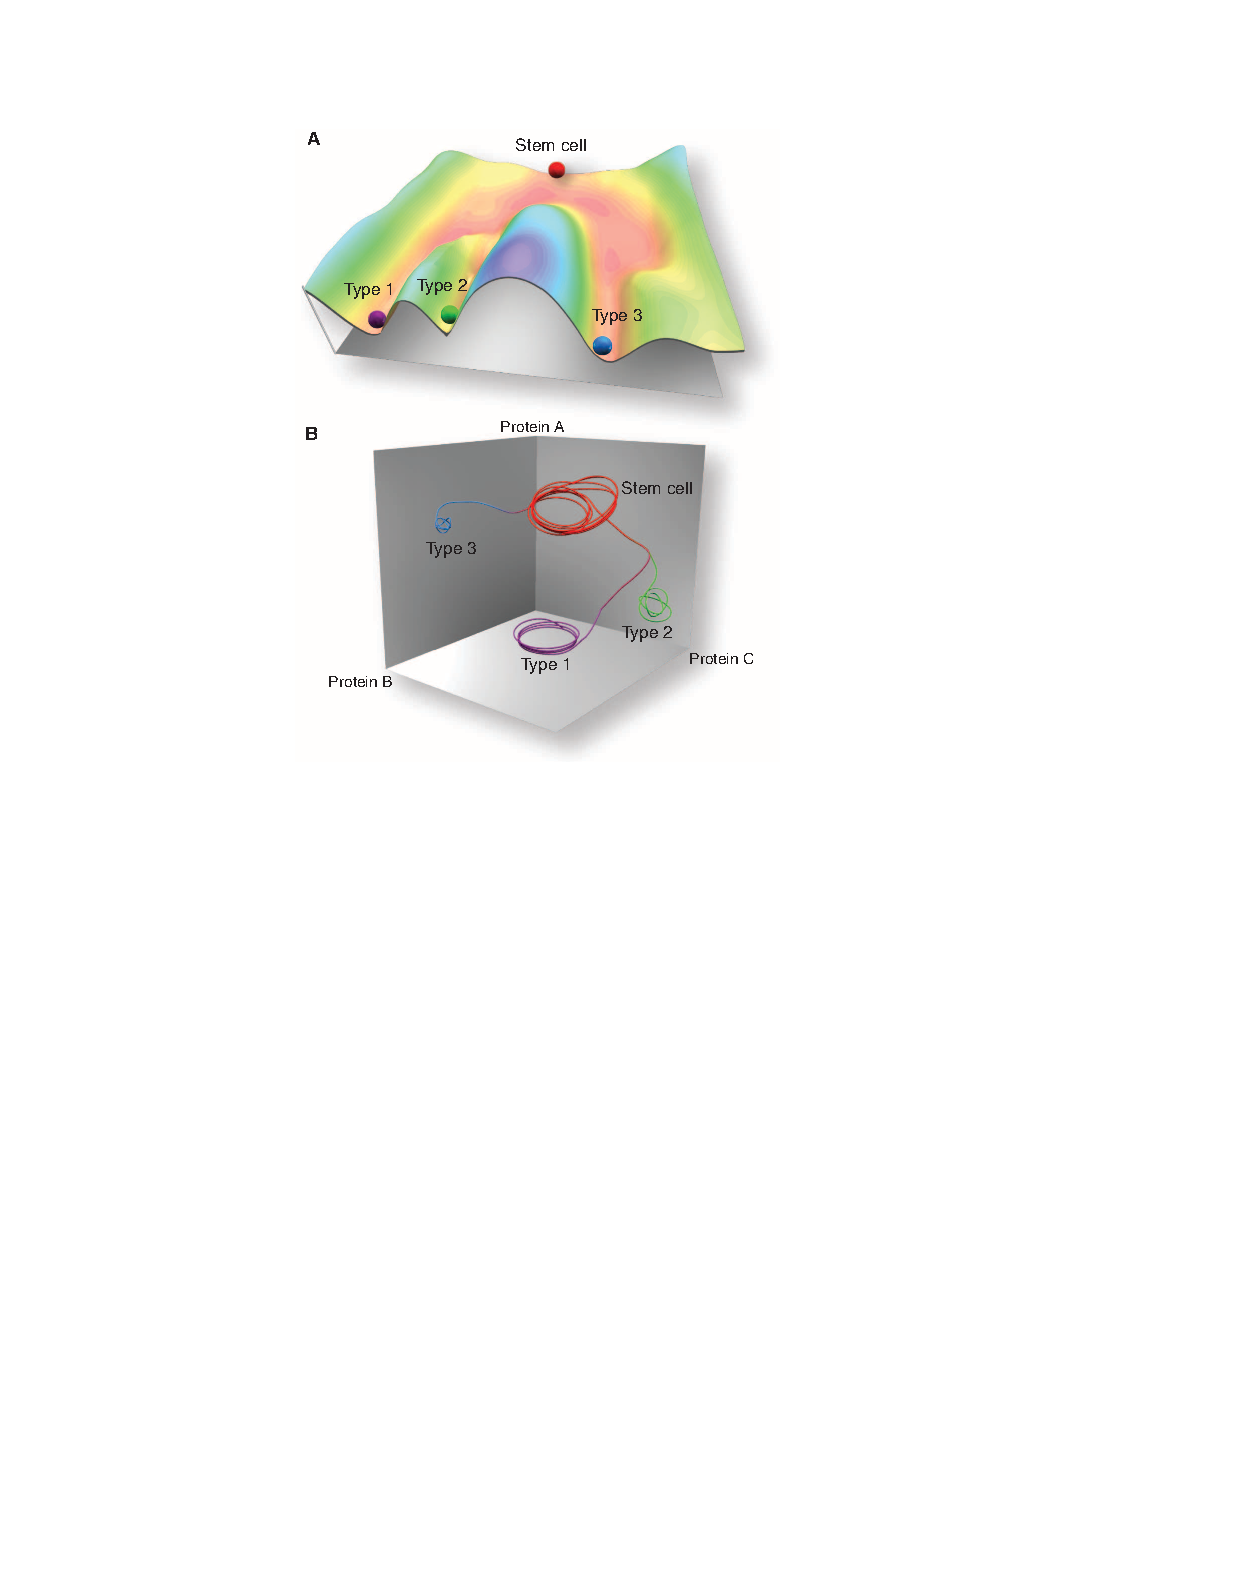
\includegraphics[width=0.5\textwidth]{figures/furusawa-epigenetic-landscape.pdf}
\captionbf{Le paysage de la diff�renciation cellulaire}{
   Figure tir�e de \cite{Furusawa2012p3898}.
   \textbf{A.} Paysage �pig�n�tique tel qu'imagin� par Waddington
   \cite{waddington1957strategy} en r�sonance avec la notion de paysage
   �nerg�tique en physique. Le d�veloppement cellulaire est repr�sent�
   par une bille d�valant un paysage compos� de diff�rentes vall�es s�par�es
   par des barri�res montagneuses, repr�sentant les diff�rents types
   cellulaires et leur robustesse face aux fluctuations.  
   \textbf{B.} Repr�sentation dynamique de l'�volution des �tats cellulaires.
   Le ph�notype est ici caract�ris� par l'expression de
   trois prot�ines A, B et C, dont l'�volution dans le temps peut �tre
   repr�sent�e par une trajectoire dans un espace tridimensionnel.
   Les �tats souche et diff�renci�s sont caract�ris�s par des bassins
   d'attraction correspondant � diff�rents types cellulaires.
} 
\label{fig:furusawa-epigenetic-landscape}
\efig

L'acquisition d'un ph�notype cellulaire particulier au sein d'un organisme est
le sujet de la biologie du d�veloppement. Cette acquisition passe par
diff�rentes �tapes de diff�renciation cellulaire. Ainsi, au cours du
d�veloppement d'un organisme, les cellules empruntent un chemin unidirectionnel
de diff�renciation qui restreint peu � peu le nombre de types cellulaires
qu'elles peuvent potentiellement devenir, passant d'un �tat souche totipotent��
des �tats pluripotents successifs avant la diff�renciation finale. Ainsi, la
formation des cellules somatiques, qui sont les cellules du corps n'�tant ni
souches ni germinales (cellules donnant naissance aux gam�tes ou cellules
sexuelles), est le r�sultat d'un processus de diff�renciation initial au cours
duquel les cellules souches donnent naissance � trois couches de tissus
distinctes : l'endoderme (feuillet interne), l'ectoderme (feuillet externe) et
le m�soderme (feuillet interm�diaire). Des diff�renciations successives ont
ensuite lieu au sein de ces couches pour former divers organes tels que le tube
digestif (endoderme), les muscles ou les os (m�soderme), la peau et le syst�me
nerveux (ectoderme).

Dans un �crit aujourd'hui c�l�bre datant de 1957 \cite{waddington1957strategy},
Waddington proposa une repr�sentation de ces diff�rentes �tapes sous la forme
d'un paysage �pig�n�n�tique semblable aux paysages �nerg�tiques dont sont
coutumiers les physiciens (fig~\ref{fig:furusawa-epigenetic-landscape}A).  Dans
cette repr�sentation, le processus de diff�renciation cellulaire est compar�
� une bille d�valant une pente et dont la trajectoire suit les multiples
embranchements de vall�es escarp�es, chacune repr�sentant un �tat de
d�veloppement diff�rent.  Les vall�es sont s�par�es par des pics dont la
hauteur refl�te la difficult� de passer d'un �tat � un autre, et les
destinations finales possibles de la bille correspondent aux diff�rents types
cellulaires.

La notion de trajectoire de diff�renciation peut �tre rendue plus parlante en
adoptant une repr�sentation de syst�me dynamique. Comme nous l'avons vu en
\ref{sub:phenotype}, la cellule contient de nombreux composants : g�nes,
prot�ines ou encore m�tabolites, qui pris dans leur ensemble d�terminent � un
instant donn� l'�tat cellulaire. Il est ainsi possible de repr�senter l'�tat
cellulaire � un temps donn� comme un point dans un espace de grande dimension
dans lequel chaque axe repr�sente l'abondance d'un certain composant
(fig~\ref{fig:furusawa-epigenetic-landscape}B). De mani�re habituelle,
l'expression des prot�ines (et donc des g�nes qui les produisent) domine ces
composants, et on parle de \og niveau d'expression g�n�tique \fg pour d�crire
leur abondance. Les changements d'expression g�n�tique, au cours desquels
certains g�nes vont �tre activ�s et d'autres r�prim�s, causent un changement de
l'�tat cellulaire, ce qui se traduit par une trajectoire dans l'espace d'�tats.
Ces changements d'expression restreignent finalement l'�tat cellulaire � une
certaine r�gion, d�finie comme un \og attracteur \fg de la dynamique. Une fois
au sein d'un attracteur, l'�tat cellulaire est robuste aux perturbations du
niveau d'expression g�n�tique des diff�rentes composantes. Les attracteurs
peuvent alors �tre vu comme des types cellulaires distincts correspondant aux
diff�rentes vall�es de la repr�sentation de Waddington
\cite{kaufmann1993origins}.


\subsection{La cellule dans l'organisme : une sp�cification spatio-temporelle}

\bfig
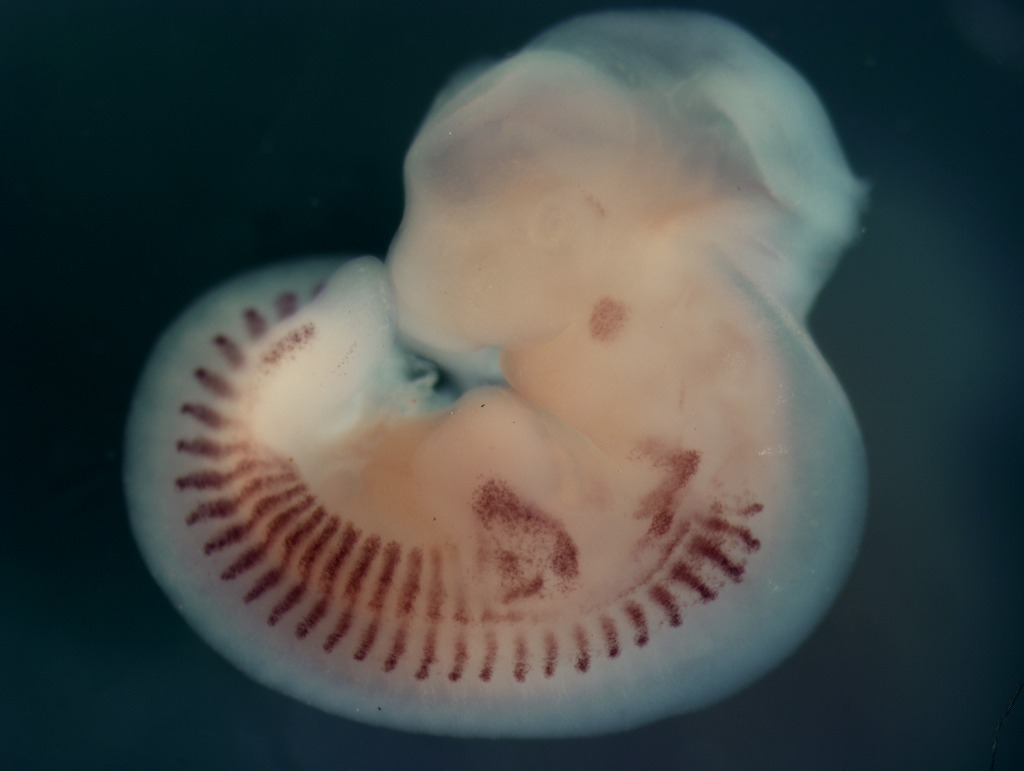
\includegraphics[width=.4\textwidth]{figures/embrys-myog.jpg}
\captionbf{Sp�cification spatio-temporelle du type cellulaire}{ 
    
    Hybridization \insitu de \myog, marqueur des cellules musculaires
    squelettiques diff�renci�es, chez un embryon de souris de $11.5$ jours. Le
    pattern de sp�cification des cellules myog�niques est clairement visible au
    niveau des futures vert�bres. L'image est tir�e de la base de donn�e Embrys
    disponible sur \url{http://embrys.jp}.

} 
\label{fig:embrys-myog}
\efig

Un fait remarquable � propos de la diff�renciation cellulaire est que celle-ci
op�re � un rythme pr�cis et dans un contexte cellulaire bien d�fini. Aussi, les
trajectoires dans l'espace d'expression g�n�tique que nous avons pr�sent�es
pr�c�demment sont fonction de l'espace -- la position de la cellule dans
l'organisme, qui d�termine en particulier la concentration des signaux qu'elle
re�oit -- et du temps -- les �tapes de d�veloppement se succ�dant de mani�re
irr�versible --. Ainsi, la diff�renciation des cellules observe certains
\textit{patterns} spatio-temporels bien d�finis : par exemple, dans le cas de
la formation des muscles, le marqueur des cellules du muscle squelettique \myog
est exprim� chez la souris d�s $8$ jours embryonnaires au niveau des somites,
les futures vert�bres de la souris adulte (voir fig~\ref{fig:embrys-myog}).


\subsection{La reprogrammation cellulaire} 
%Fibroblastes, IPS : seulement un ou quelques facteurs suffisent � changer le
%ph�notype d'une cellule.

\bfig
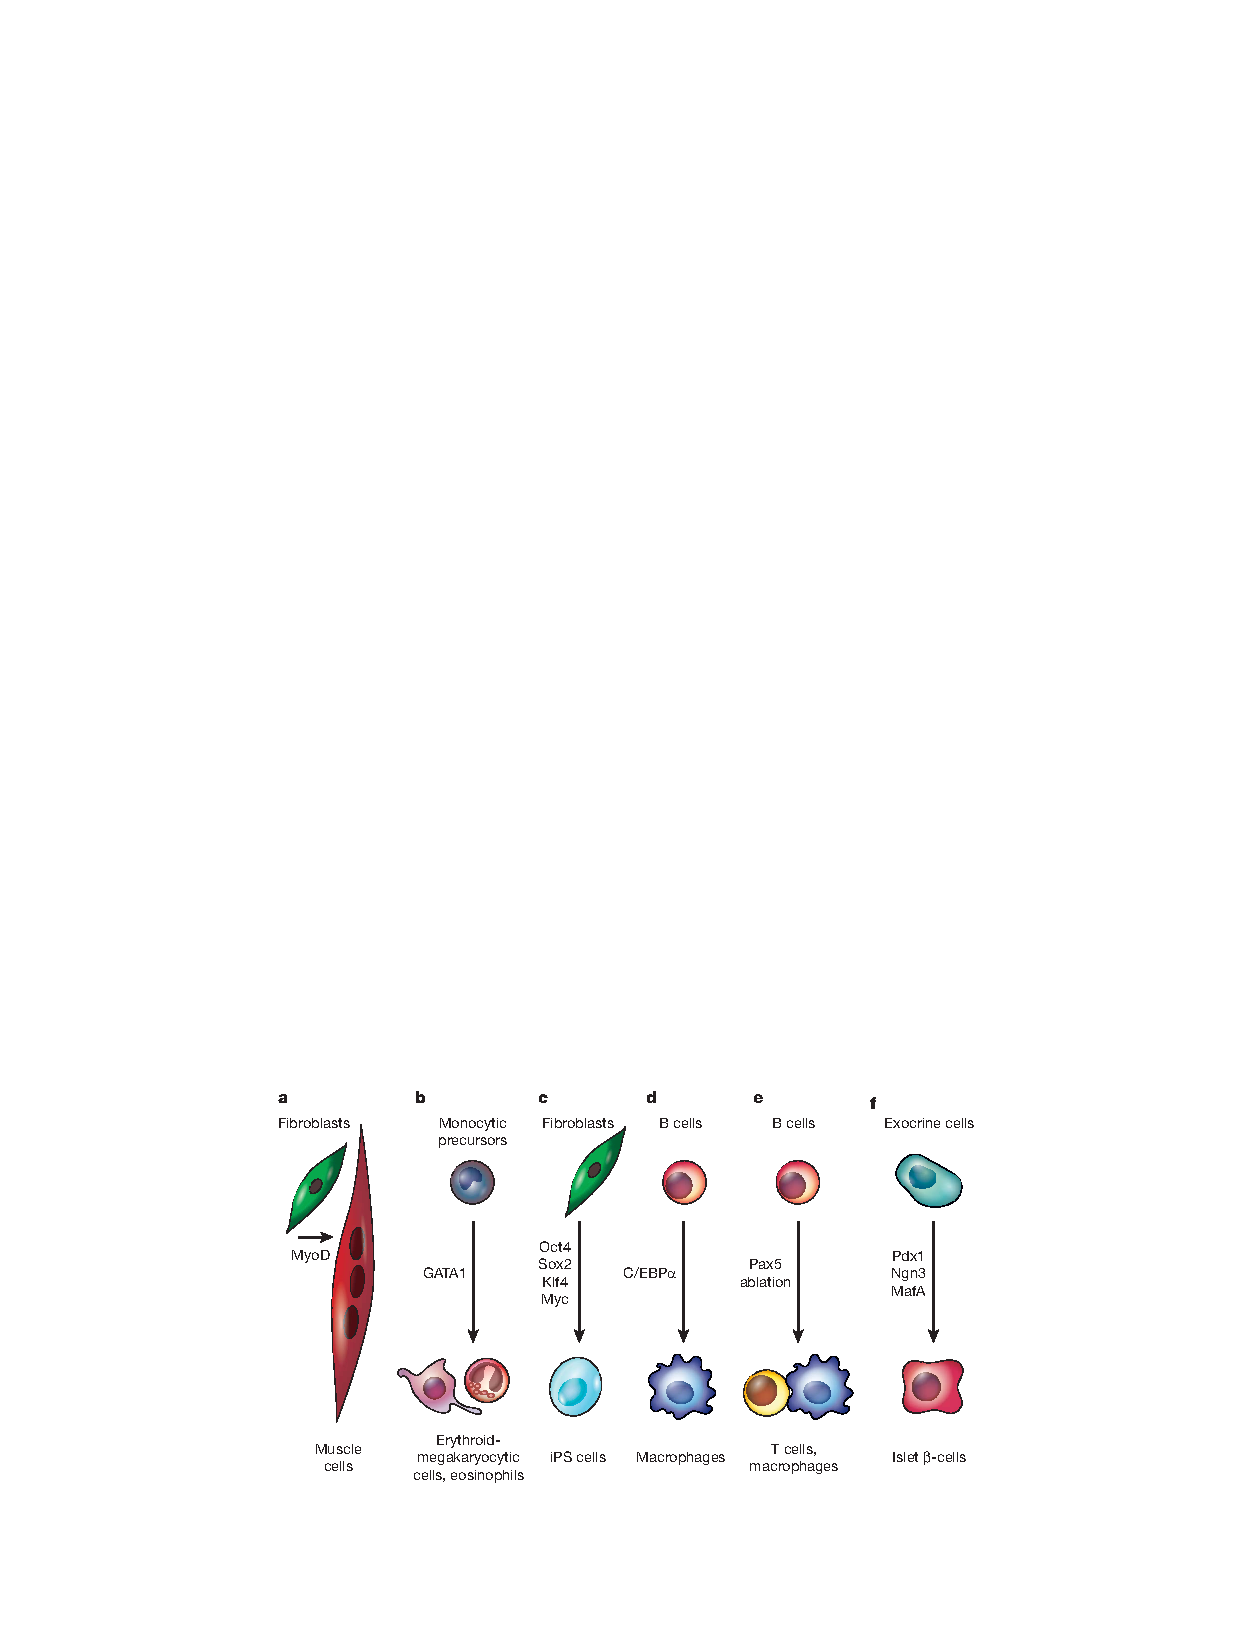
\includegraphics[width=\textwidth]{figures/graf-cells-lineages.pdf}
\captionbf{Diff�rents exemples de reprogrammation cellulaire}{
    Figure tir�e de \cite{Graf2009p2592}. Exemples d'exp�riences de
    surexpression ou d'ablation de \fts qui aboutissent � des changements de
types cellulaires.  } \label{fig:graf-cells-lineages} \efig 

Dans les paragraphes pr�c�dents, nous avons pr�sent� la vision classique selon
laquelle des cellules souches totipotentes se diff�rencient en des cellules de
moins en moins plastiques, jusqu'� atteindre un �tat diff�renci� stable.
N�anmoins, depuis plusieurs d�c�nies, diff�rentes exp�riences ont exhib� la
plasticit� des �tats diff�renci�s. Par exemple, Blau et al. ont montr� en
1985 que des programmes d'expression g�n�tiques dormants peuvent �tre exprim�s
de mani�re dominante dans des cellules diff�renci�es par la fusion de
diff�rents types cellulaires \cite{Blau1985vn}. Puis diff�rents travaux ont
montr� qu'il �tait possible de convertir des lign�es de cellules en introduisant
certaines prot�ines r�gulatrices de la transcription, ou \FTs (TFs)
\cite{davis1987expression,Kulessa1995ys} (voir fig
\ref{fig:graf-cells-lineages}).  Parall�lement, des exp�riences r�alis�es chez
plusieurs esp�ces ont montr� que le transfert de noyaux de cellules
diff�renci�es embryonnaires ou adultes dans un oeuf �nucl�� peut mener � la
formation d'un organisme complet, montrant de mani�re univoque que l'identit�
des cellules diff�renci�es peut �tre compl�tement
renvers�e~\cite{Gurdon2008zr}. Enfin, l'avanc�e la plus r�cente dans ce
domaine a �t� la d�monstration que des cellules somatiques diff�renci�es
peuvent �tre reprogramm�es en cellules souches puripotentes par simple
introduction d'un cocktail de 4 \tfs~\cite{Takahashi2006kx} (fig
\ref{fig:graf-cells-lineages}C).


\section{Les r�seaux de r�gulation g�n�tique}

Afin de pouvoir mieux comprendre les m�canismes de diff�renciation et de
reprogrammation expos�s en~\ref{sec:phenotype}, il convient de se plonger dans
les m�canismes internes de la cellule qui r�gissent ses changements d'�tats.

\subsection{Vision cybern�tique de la cellule}

\bfig 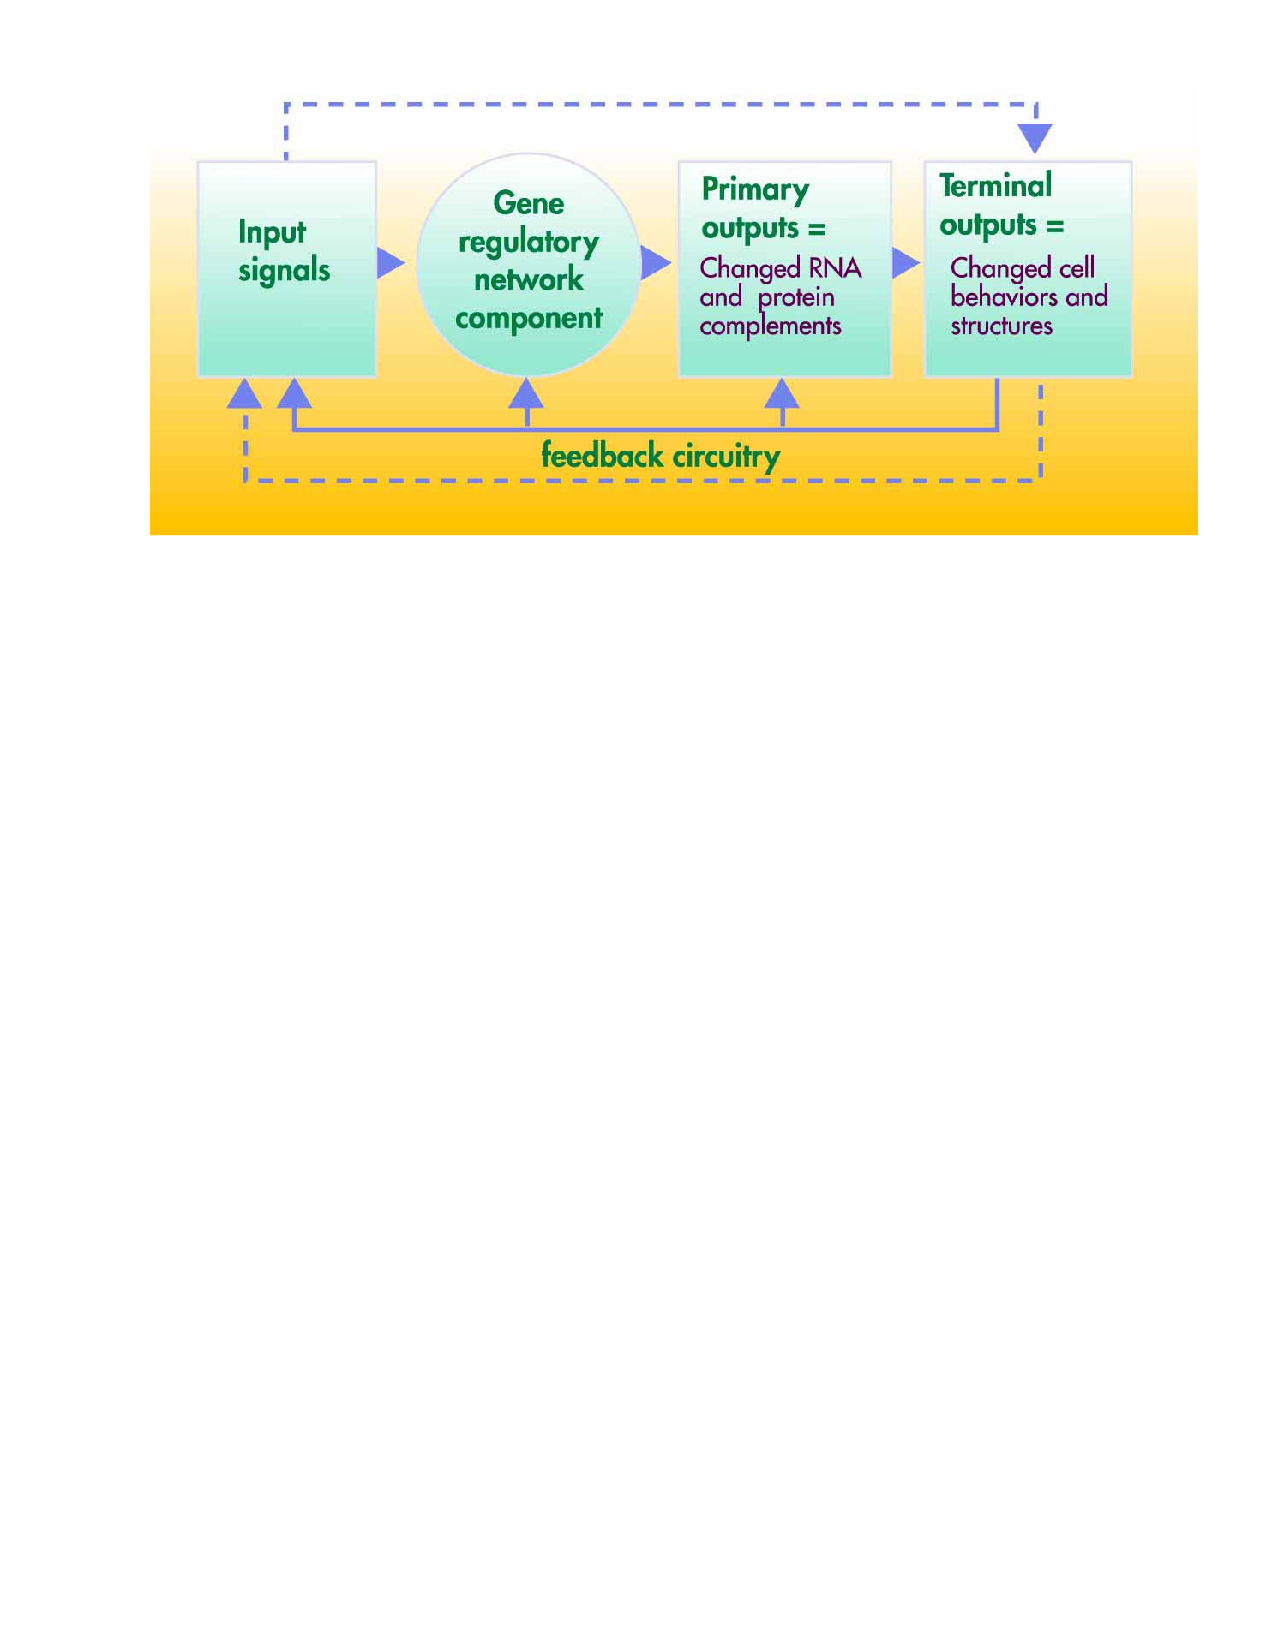
\includegraphics[width=\textwidth]{figures/us-cybernetics.pdf}
\captionbf{Vision cybern�tique du traitement de l'information par la cellule}{
    Figure tir�e du programme ``Genomes to life'' du D�partement de l'�nergie
    des �tats-Unis datant de 2001 \cite{USDE} sch�matisant un r�seau
    de r�gulation cellulaire comme un syst�me de traitement entr�e/sortie,
    poss�dant trois composantes fondamentales : (1) un syst�me de r�ception et
    de transduction des signaux d'entr�es qui peuvent �tre intra- ou
    extra-cellulaires (plusieurs signaux pouvant affecter un m�me g�ne cible),
    (2) un ``composant central'' (\textit{core component}) compos� du r�seau de
    r�gulation g�n�tique traitant les signaux, et (3) de l'expression mol�culaire
    des ARNs et prot�ines des g�nes cibles observ�e en sortie. Le processus r�sulte
    en la modification du ph�notype ou de la fonction de la cellule. Des boucles de
    r�gulation (\textit{feedback}) assurent le contr�le et la stabilit� des
diff�rentes �tapes.
} \label{fig:us-cybernetics} \efig


Le paradigme qui r�gne sur la biologie mol�culaire depuis plus d'un demi si�cle
est celui des r�seaux g�n�tiques. L'expression est g�nes est en effet r�gul�e
par des prot�ines, les \fts, qui sont elles-m�mes exprim�es par d'autres g�nes,
cr�ant ainsi des interactions entre g�nes.  Par ailleurs, les prot�ines peuvent
r�guler l'activit� d'autres prot�ines, et certains ARN issus de la
transcription de g�nes non codants op�rent aussi de mani�re primordiale dans la
r�gulation de l'activit� g�n�tique, le tout formant un r�seau complexe
d'interactions. La compr�hension de ce r�seau et des fonctions qu'il englobe
forme le socle de la discipline de biologie des syst�mes. Dans ce cadre, la
cellule est vue comme une machine interpr�tant diff�rents signaux re�us en
entr�e et qui, une fois trait�s par le r�seau interne de r�gulation, r�agit en
sortie en modifiant son �tat ou son comportement
(fig~\ref{fig:us-cybernetics}). L'int�r�t d'une telle description m�canistique
est qu'elle permet d'op�rer quantifications math�matiques et pr�dictions, ce
qui l'a rendue extr�mement fertile au cours des derni�res d�cennies
\cite{Nurse2011p2308}.

\subsection{Divers modes de r�gulation}
\label{sub:divers_modes_de_regulation}

\bfig 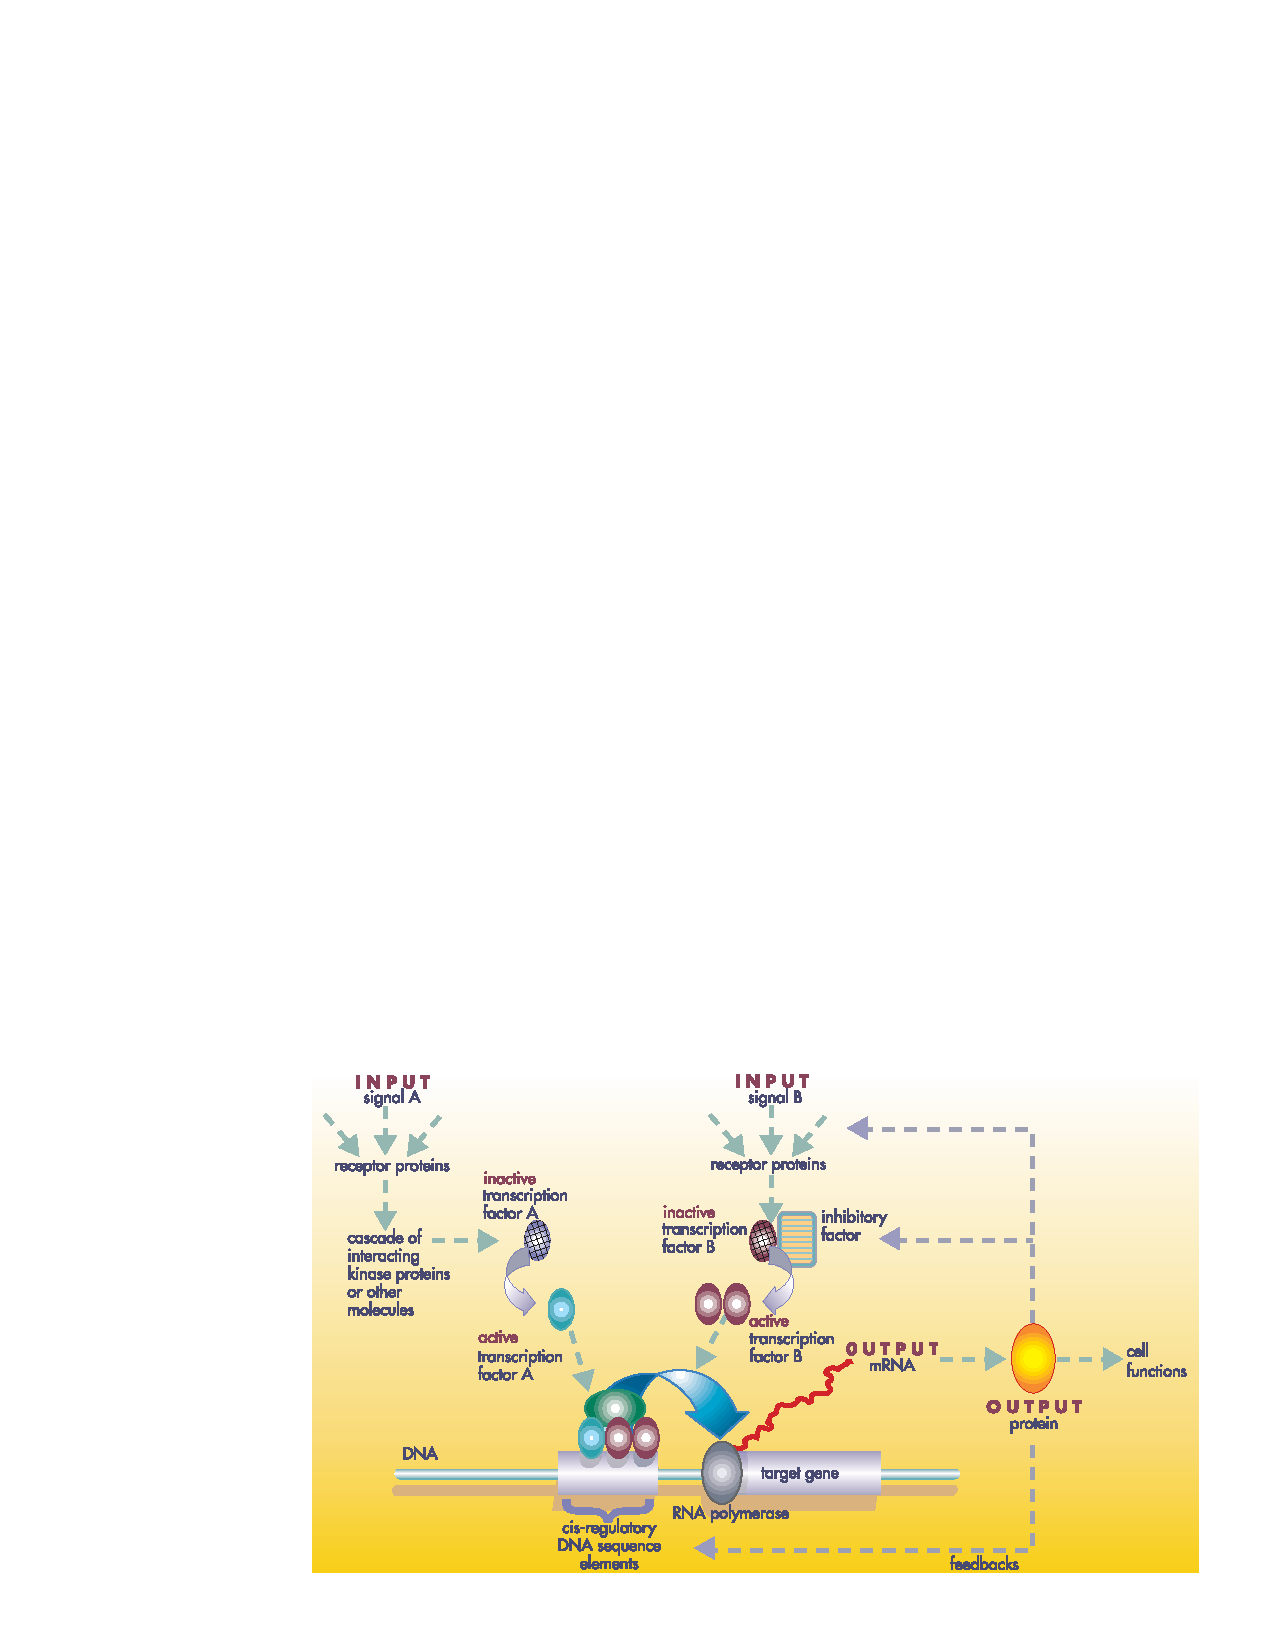
\includegraphics[width=1.0\textwidth]{figures/us-grn.pdf} \captionbf{Un
r�seau de r�gulation g�n�tique type}{ Dans cette repr�sentation sch�matique
    tir�e de \cite{USDE}, deux voies de signalisation A et
    B transmettent des signaux d'entr�e (qui peuvent �tre intra ou extra
    cellulaires)  en activant des \fts.  Une fois activ�s, ces derniers
    interagissent avec des s�quences d'ADN proches d'un g�ne cible en se fixant
    sur des sites de petite taille ($\sim10$bp).  Les diff�rents \tfs
    interagissent entre eux pour former des complexes occupant des r�gions de
    $\sim1000$bp appel�es \crms ou CRMs.  Lorsque les \tfs sont fix�s sur le
    CRM de leur g�ne cible, il peuvent activer ou inhiber la transcription
    d'ARN et donc la production de la prot�ine correspondante.}
    \label{fig:us-grn} \efig

Les modes de r�gulation qui permettent � la cellule d'interpr�ter des signaux
et de changer d'�tat sont nombreux. Nous allons nous concentrer ici sur ceux
internes aux r�seaux g�n�tiques, et affectant au final la production de
prot�ines ou d'ARNs et donc l'�tat cellulaire (fig.~\ref{fig:us-grn}).

\subsubsection{R�gulation g�n�tique}

Tout d'abord, un r�seau d'expression g�n�tique est caract�ris� par un jeu
d'interactions entre diff�rents g�nes. Ces interactions se font par
l'interm�diaire de prot�ines r�gulatrices appel�es \fts ou TFs, qui sont au
nombre de $\sim1400$ chez l'homme \cite{Vaquerizas2009ys}, soit $6\%$ des
prot�ines encod�es. Les g�nes qui les expriment repr�sentent donc $\sim3$\% de
l'ensemble des $30,000$ g�nes connus � ce jour. Pour r�guler (activer ou
inhiber) la transcription d'un g�ne cible, les TFs se fixent sur des sites de
reconnaissance sp�cifiques sur l'ADN de $\sim10$bp et interagissent avec la
machinerie transcriptionnelle au niveau du promoteur du g�ne cible. Les TFs
peuvent se fixer sur le promoteur m�me, comme c'est souvent le cas chez la
bact�rie, ou dans des r�gions distales allant jusqu'� plusieurs centaines de
kb, comme on trouve plus couramment chez les organismes complexes. Par
ailleurs, diff�rents TFs peuvent se combiner sur certaines r�gions de
r�gulation contenant de multiples sites de fixation pour former des complexes
prot�iques.  Ces r�gions, appel�es \crms (CRMs) ou plus commun�ment
\textit{enhancers}, sont d'une taille typique de $\sim1000$bp et ont la
particularit� de conduire � une expression spatio-temporelle tr�s sp�cifique du
g�ne cible. Ces diff�rents points seront amplement d�velopp�s en
section~\ref{sec:CRMs}.

\subsubsection{R�gulation �pig�n�tique} 

\bfig
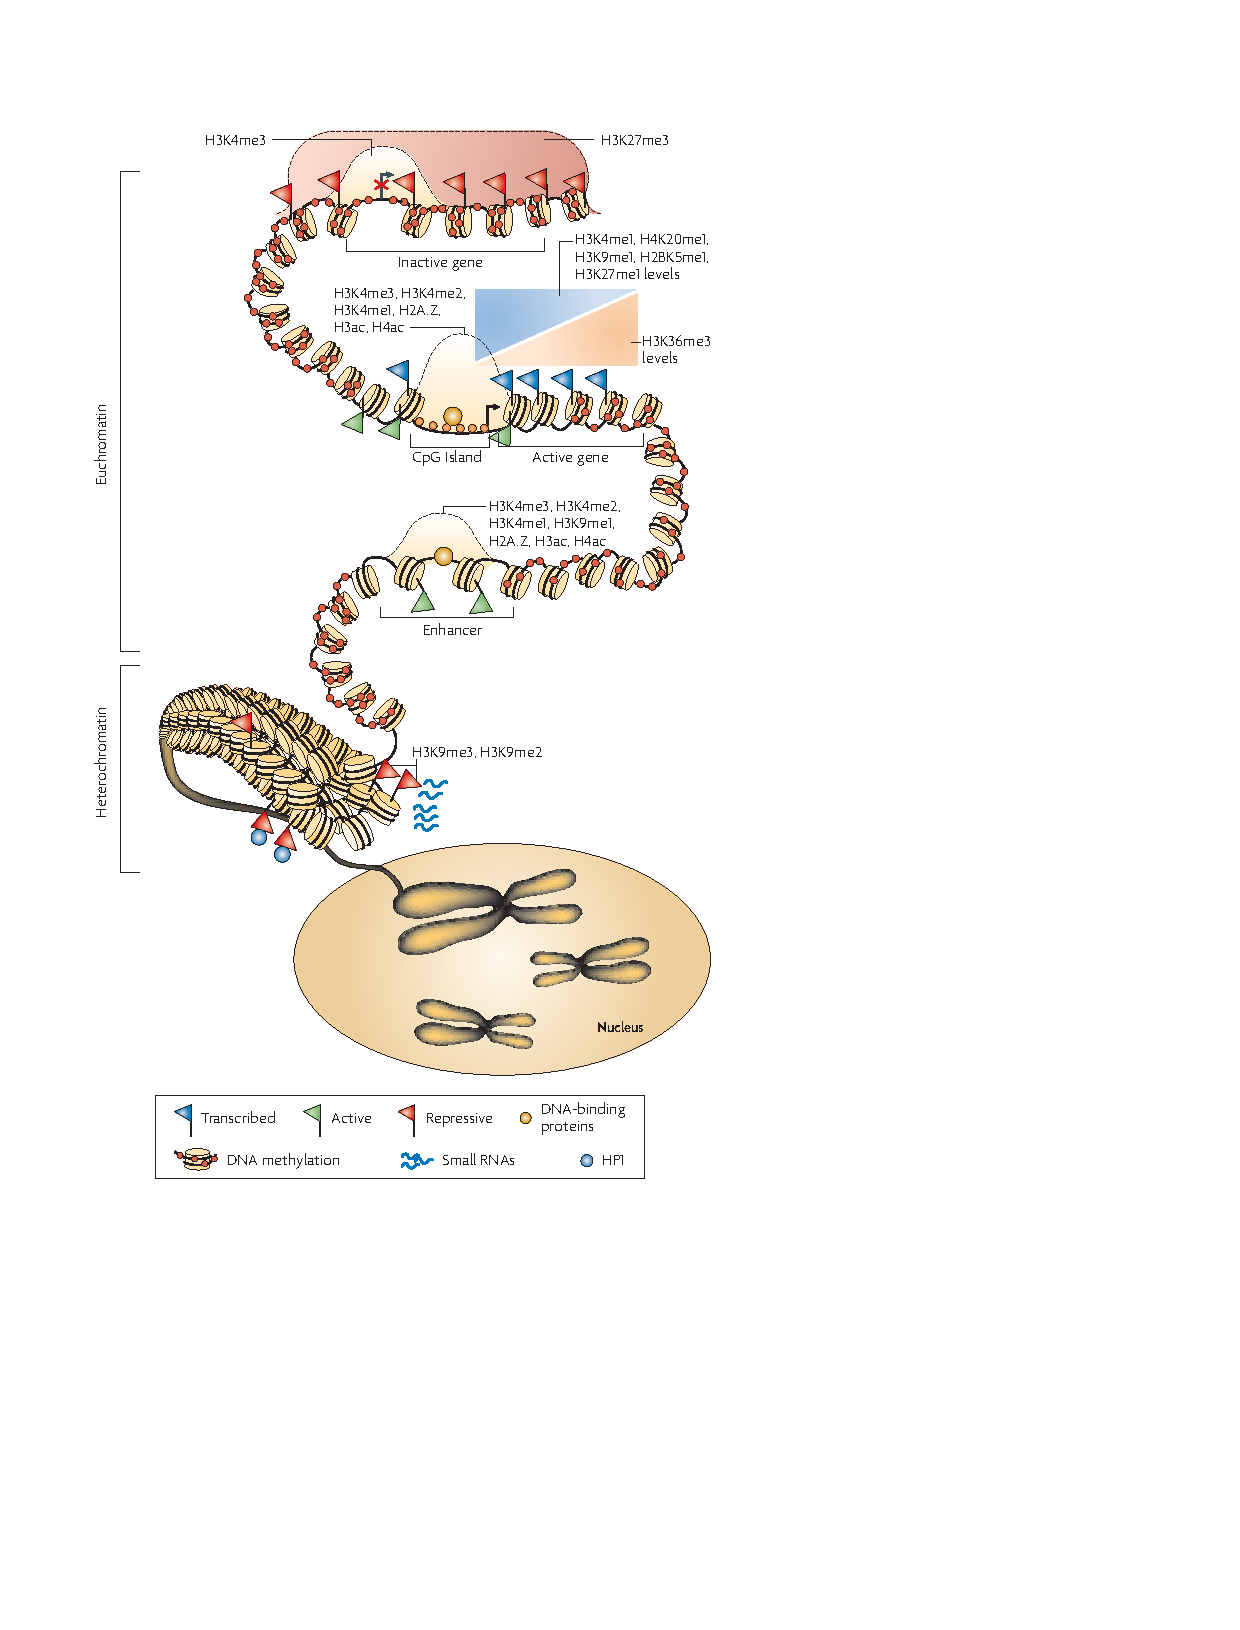
\includegraphics[width=0.7\textwidth]{figures/schones-epigenome.pdf}
\captionbf{Caract�ristiques de l'�pig�nome}{ Figure tir�e
    de~\cite{Schones2008nx}. Les chromosomes sont partag�s entre r�gions
accessibles d'euchromatine et r�gions difficilement accessibles
d'h�t�rochromatine. Les r�gions h�t�rochromatiques sont marqu�es par de la di-
et trim�thylation de la lysine 9 de l'histone H3 (H3K9me2 et H3K9me3). La
m�thylation de l'ADN est pervasive � travers le g�nome et est seulement absente
dans les r�gions telles que les �lots CpG, les promoteurs et les CRMs. La
modification H3K27me3 couvre de larges r�gions englobant des g�nes inactifs.
Les marques H3K4me3, H3K4me2, H3K4me1 et l'ac�tylation des histones marquent
les TSSs des g�nes actifs. Les marques H3K4, H3K9, H3K27, H4K20 et H2BK5
marquent les r�gions transcrites activement � proximit� de la r�gion 5' des
g�nes (en aval), alors que la marque H3K36 marque les g�nes transcrits dans
leur r�gion 3' (en amont). } \label{fig:schones-epigenome} \efig


Outre la r�gulation g�n�tique, due � l'action de prot�ines issues de s�quences
codantes et se fixant sur des s�quences d'ADN, r�gulation qui est donc
enti�rement encod�e dans le g�nome et transmise � la descendance, il existe un
autre mode de r�gulation de la transcription des g�nes qui permet notamment
d'acqu�rir une modification d'expression g�n�tique transmise � la descendance
sans qu'il y ait modification du code g�n�tique : on parle de r�gulation
�pig�n�tique. Cette r�gulation passe notamment par la modification des
propri�t�s chimiques de l'ADN et des histones sur lequel il s'enroule pour
former la chromatine. Ainsi, la m�thylation des dim�res CpG de
l'ADN\footnote{Les dim�res C-G sont appel�s CpG, o� p caract�rise le phosphore
liant les deux bases, pour les diff�rencier du CG utilis� pour parler de la
statistique en C et G de l'ADN} au niveau des r�gions riches en CG, ou �lots
CpG, situ�es pr�s de nombreux promoteurs et habituellement d�pourvues de ces
marques conduit � une inactivation du g�ne cible~\cite{Bird2002oq}.  Par
ailleurs, la m�thylation des histones au niveau des r�sidus lysines entra�ne la
fermeture de la chromatine, emp�chant l'expression du ou des g�ne(s) situ�s
� leur niveau, alors que l'ac�tylation des m�mes lysines entra�ne au contraire
une ouverture de la chromatine, favorisant ainsi la transcription
g�n�tique~\cite{Greer2012ve}.  Ce mode de r�gulation sera d�velopp� plus en
d�tails en section~\ref{sub:les_diff_rents_types_de_crms}.

% lincRNAs? \cite{Rinn2012p3940}

\subsubsection{R�gulation post-transcriptionnelle} 

Les modifications post-transcriptionnelles affectent les ARNs issus de la
transcription des g�nes. Ces modifications peuvent �tre caus�es par des ARNs
doubles brins ou dsRNA (\textit{double-stranded RNAs)} qui, une fois cliv�s par
la prot�ine Dicer, forment des petits peptides de 22 nts appel�s siRNAs
(\textit{small interfering RNAs)}) qui recrutent le complexe prot�ique RISC
(\textit{RNA-induced silencing complex}) et ciblent sp�cifiquement des
ARNm~\cite{Hammond2001bh,Hannon2002qf}. Cette m�thode est connue sous le nom
d'interf�rence ARN (RNAi) et est aujourd'hui couramment utilis�e pour inhiber
l'expression d'un g�ne. De mani�re similaire, les microARNs ou miRNAs sont des
ARNs de $\sim23$ nts issus d'ARNs plus longs appel�s \og �pingles � cheveux \fg
ou \textit{hairpins} qui s'associent � la prot�ine \textit{Argonaute} du
complexe RISC pour entra�ner la d�gradation sp�cifique
d'ARNms~\cite{Bartel2009cr}.




\subsubsection{R�gulation post-traductionnelle}

Les modifications post-traductionnelles affectent les prot�ines issues de la
traduction des ARNs. Ces modifications passent par une modification chimique
des prot�ines, typiquement la phosphorylation, ou comme nous l'avons vu pour la
r�gulation �pig�n�tique, la m�thylation ou l'ac�tylation. Ces modifications
peuvent avoir pour effet de changer l'activit� de la prot�ine, que ce soit en
modifiant son activit� enzymatique ou en d�clenchant sa relocalisation
nucl�aire. Par ailleurs, il existe aussi des modifications de structure de la
prot�ine, comme c'est le cas du \tf \textit{Shavenbaby} chez la Drosophile:
dans sa forme native, cette prot�ine inhibe la transcription de ses g�nes cible
; cependant ses r�sidus terminaux peuvent �tre cliv�s par des petits peptides
de 11 � 32 acides amin�s encod�s par le g�ne \textit{Pri}, rendant la prot�ine
transcriptionnellement active \cite{Kondo2010ly}.

\subsection{C�blage du r�seau et fonction}

\bfig
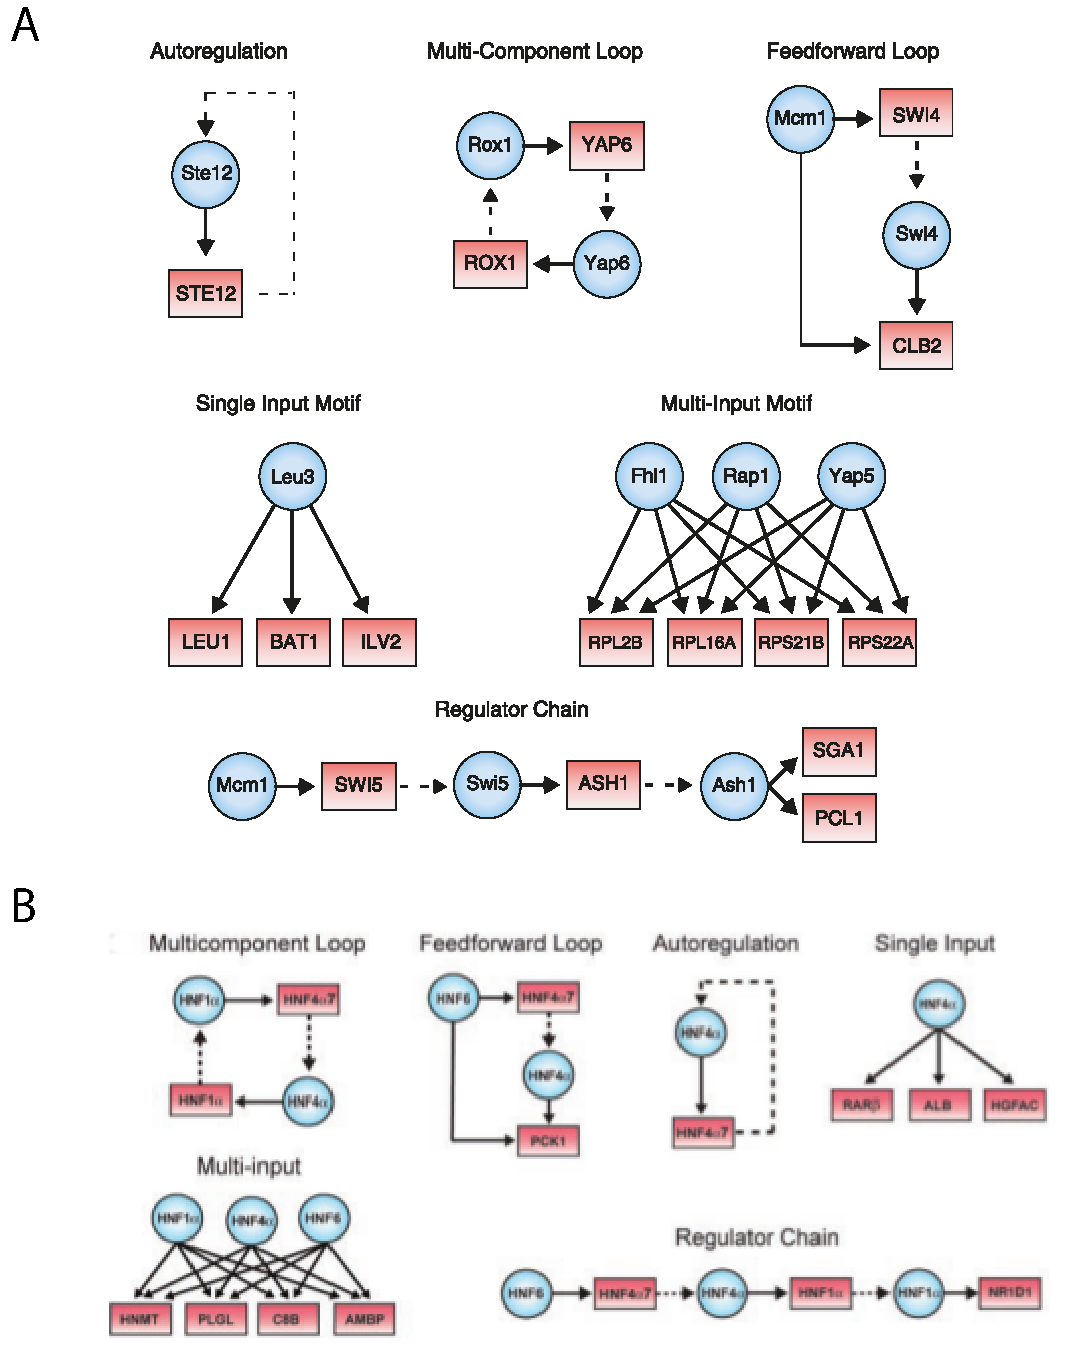
\includegraphics[width=0.7\textwidth]{figures/lee-network-motifs-yeast.pdf}
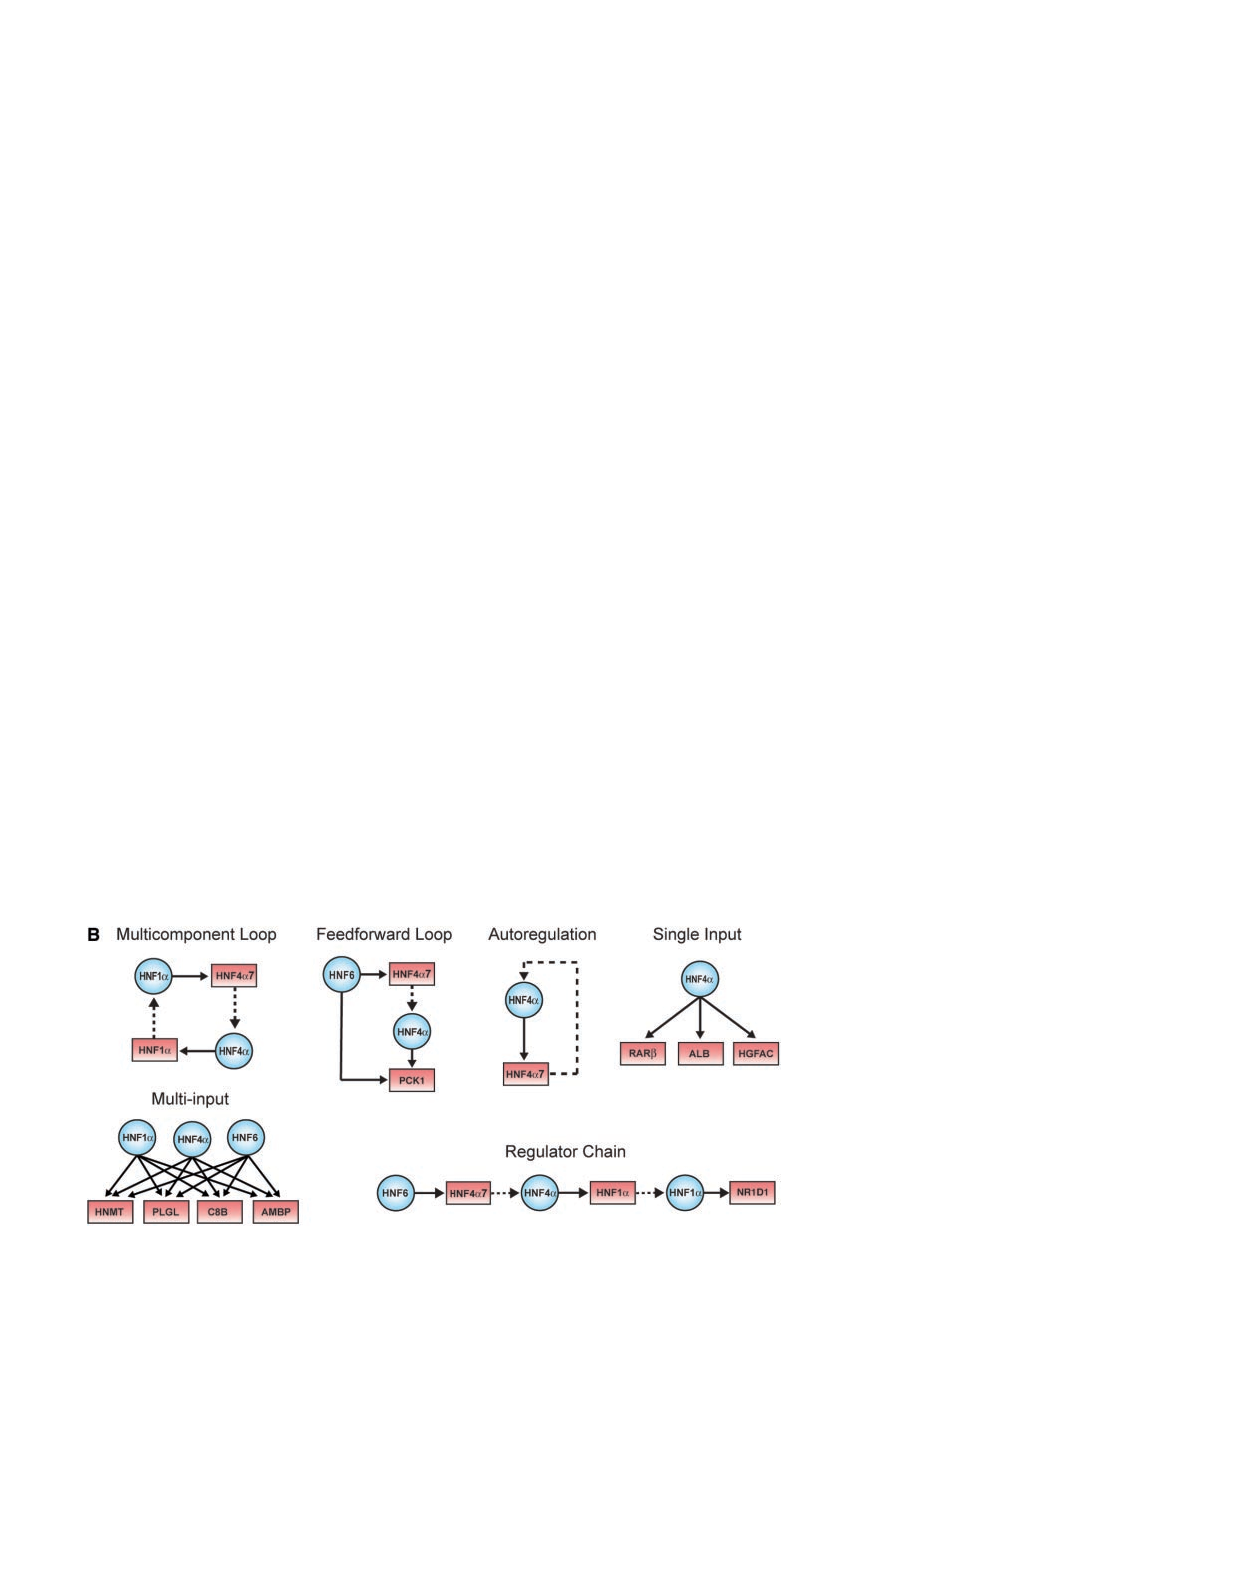
\includegraphics[width=0.9\textwidth]{figures/odom-network-motifs-human.pdf}
\captionbf{Exemples de motifs dans les r�seaux de r�gulation g�n�tique}{Figure
    tir�e de .  Ces exemples sont issus d'analyses d'interactions entre \tfs
    (cercles bleus) et promoteurs (rectangles rouges) chez la
    levure~\cite{Lee2002p537} (A) et chez l'homme~\cite{Odom2004hc} (B).  Les
fl�ches solides indiquent la fixation d'un \tf � un promoteur, et les fl�ches
en pointill� indiquent l'expression d'un \tf � partir de son g�ne.}
\label{fig:lee-odom-networks}\efig

Maintenant que nous avons vu la nature des interactions au sein des r�seaux
g�n�tiques, nous pouvons nous pencher sur leur structure. Celle-ci est en effet
loin d'�tre due au hasard. Ainsi, plusieurs �tudes, r�alis�es chez divers
organismes de la bact�rie � l'homme, ont r�v�l� que les r�seaux de
transcription contiennent un petit ensemble de motifs de r�gulation r�currents,
appel�s motifs de
r�seaux~\cite{alon2007introduction,ShenOrr2002p648,Milo2002tg}
(fig.~\ref{fig:lee-odom-networks}).  Ces motifs peuvent �tre vus comme les
pi�ces �l�mentaires servant � la construction de r�seaux fonctionnels. De tels
motifs furent d'abord d�tect�s de mani�re syst�matique chez la bact�rie \ecoli
en remarquant qu'ils apparaissaient dans le r�seau de transcription bien plus
souvent qu'on ne l'attendrait dans un r�seau al�atoire~\cite{ShenOrr2002p648}.
Les m�mes motifs ont ensuite �t� trouv�s chez la
levure~\cite{Milo2002tg,Lee2002p537} et chez l'homme~\cite{Odom2004hc}. La
r�currence de ces motifs est li�e aux fonctions qu'ils remplissent. Par
exemple, la boucle d'autor�gulation n�gative, qui est trouv�e chez la moiti�
des r�presseurs d'\ecoli, poss�de deux fonctions : l'une est de parvenir
rapidement � un �tat d'�quilibre en utilisant un promoteur fort, l'autre est de
servir de tampon au bruit d'expression~\cite{Alon2007p2353}. Un autre motif
r�current est la boucle feedforward. Celle-ci consiste en 3 g�nes : un
r�gulateur X, qui r�gule Y, tous deux r�gulant Z. Dans le cas o� des
interactions sont des activations et que X et Y sont requis pour activer Z,
cette boucle peut servir de tampon au bruit d'expression de X, �vitant que des
fluctuations de son niveau d'expression n'entra�ne par erreur l'activation de
Z.


\subsection{�volution des r�seaux g�n�tiques}

\bfig
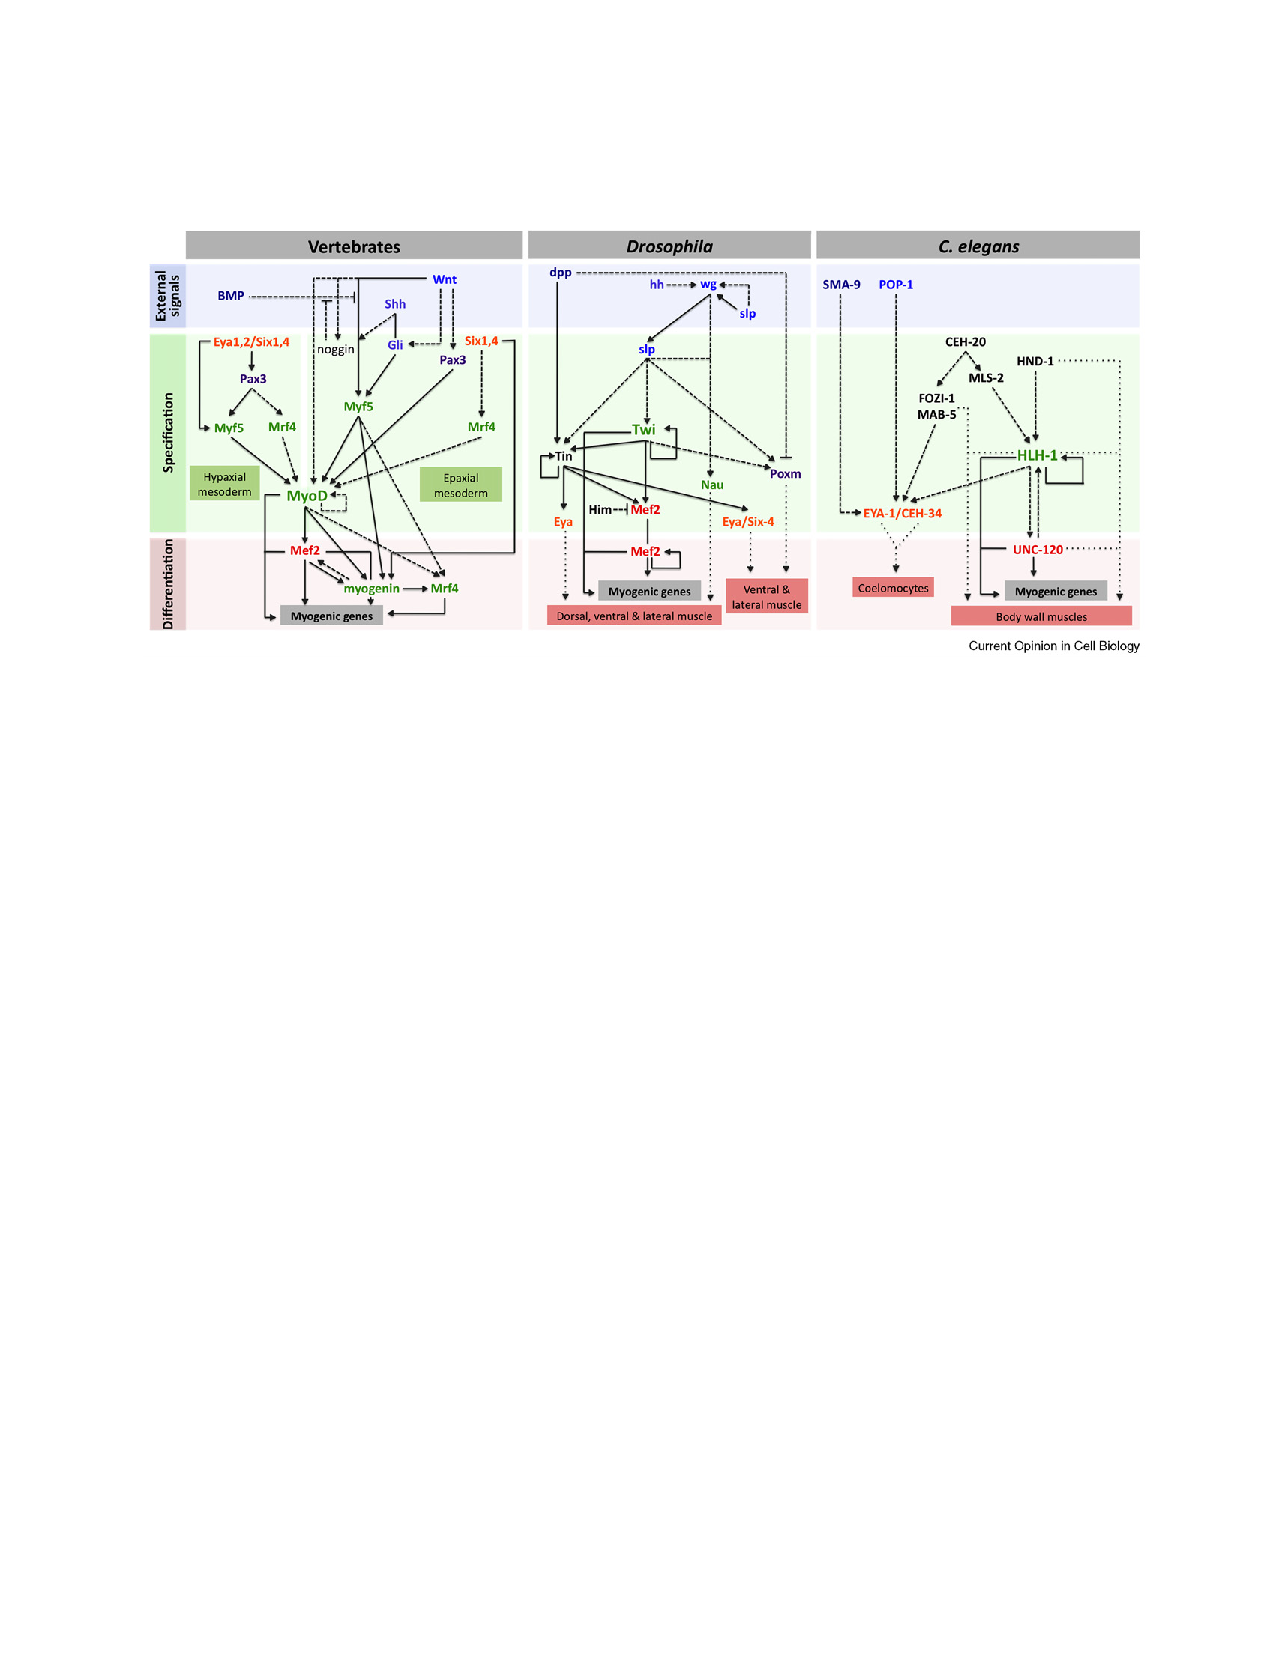
\includegraphics[width=\textwidth]{figures/furlong-network-evolution.pdf}
\captionbf{�volution du r�seau transcriptionnel : l'exemple de la r�gulation
myog�nique.}{ Figure tir�e de \cite{Liu2009p556}. Les lignes pleines indiquent
une r�gulation transcriptionnelle directe, les tirets indiquent des
interactions g�n�tiques dont le caract�re direct n'a pas �t� montr�, et les
lignes pointill�s indiquent que l'interaction est sugg�r�e par des donn�s
d'expression. \myod est l'analogue structurel de \textit{Nautilus} mais est
l'analogue fonctionnel de \textit{Twist} chez la Drosophile et de
\textit{HLH-1} chez C. Elegans. Les couleurs indiquent respectivement des voies
de signalisation externes au m�soderme (bleu), les r�gulateurs myog�niques de
la famille bHLH (vert), les prot�ines Six/Eya (orange), les prot�ines de la
famille \textit{paired-box} Pax (violet), les TFs des familles MADS/SRF
(rouge), et les r�gulateurs d'autres familles de prot�ines (noir).}
\label{fig:furlong-network-evolution}\efig

Au cours de l'�volution, les r�seaux de r�gulation g�n�tique changent
: modification des constituants, rec�blage du r�seau, duplication
d'�l�ments\ldots N�anmoins, certaines modifications sont plus d�favoris�es du
point de vue �volutif que des autres.  Par exemple, la modification d'un
r�gulateur, par exemple une mutation d'un certain acide amin� d'un \tf, aura
des cons�quences sur l'ensemble des �l�ments r�gul�s par ce \tf. Par contre, la
modification d'un site de reconnaissance de ce \tf sur l'ADN n'aura qu'une
port�e locale sur la r�gulation du g�ne associ�. Par ailleurs, certains motifs
du r�seau, comme les boucles d'autor�gulation ou les boucles feedforward,
peuvent avoir une grande importance fonctionnelle, favorisant leur
conservation. \\
� titre d'exemple, prenons le cas du r�seau de diff�renciation du muscle
squelettique pr�sent� en figure~\ref{fig:furlong-network-evolution}, que nous
�tudierons plus en d�tail dans le chapitre \ref{chap:muscle} de ce manuscrit.
Au coeur de ce r�seau g�n�tique se trouvent les facteurs de r�gulation
myog�niques ou MRFs, des \fts de type bHLH qui ont la capacit� de convertir des
cellules non mesodermales, \cad n'�tant pas destin�es � devenir des
prog�niteurs musculaires, en cellules ayant des propri�t�s
musculaires~\cite{Weintraub1989ij}. Ces facteurs sont dits \og r�gulateurs
ma�tres \fg de la diff�renciation musculaire. Chez les vert�br�s il y a quatre
MRFs: \myf, \mrf, \myod, qui ont des roles redondant dans la sp�cification des
prog�niteurs musculaires, et \myog, qui conduit � la diff�renciation terminale.
Chez la \droso c'est le TF  \twi qui semble �tre le principal MRF, mais
contrairement aux MRFs des vert�br�s, son r�le ne s'arr�te pas au contr�le de
la diff�renciation musculaire mais est plus g�n�ral dans le d�veloppement du
m�soderme~\cite{Baylies1998bs}. C'est cependant le g�ne \textit{Nautilus} qui
poss�de la s�quence d'acides amin�s la plus proche de celle des MRFs vert�br�s.
Ce dernier permet la sp�cification des prog�niteurs myog�niques, et son
expression est restreinte au d�veloppement musculaire. N�anmoins, les mutants
\textit{nautilus} sont viables et son r�le semble mineur compar� aux MRFs
vert�br�s. Enfin, chez le ver \celegans, c'est l'orthologue de \myod,
\textit{hlh-1}, qui tient r�le de MRF.\\ Malgr� ces diff�rences (nombre de
MRFs, membre de la famille bHLH tenant ce r�le), on retrouve dans les trois cas
une boucle feedforward conserv�e au niveau de la r�gulation des cibles des MRFs
(fig.~\ref{fig:furlong-network-evolution}).  Ainsi, MyoD r�gule l'expression de
Mef2 et l'activit� de MAPK p38 en m�me temps que l'expression de plusieurs
cibles initiales, et par la suite MyoD et phospho-Mef2 co-r�gulent des g�nes
plus tardifs. Ce m�canisme permet ainsi de r�guler l'aspect temporel de
l'expression g�n�tique.  Chez la Drosophile, le m�me motif est observ� avec
Twist et Mef2 et chez C.  Elegans avec HLH-1 et le TF UNC-129, de la m�me
famille que Mef2.  \\ Ainsi le coeur du r�seau est conserv� dans la forme
(topologie), m�me s'il y a des divergences dans le fond (membres de la famille
de TFs impliqu�s). N�anmoins, les �l�ments r�gulateurs en amont, ainsi que les
membres p�riph�riques du r�seau ont rapidement �volu�. Par exemple, chez les
vert�br�s le TF Pax3 est tr�s en amont dans la hi�rarchie g�n�tique et permet
l'activation des MRFs et la sp�cification myog�nique, alors que chez la
Drosophile son homologue \textit{poxm} est en aval des MRFs et sa perte de
fonction n'a que des effets mineurs sur la myogen�se. Par ailleurs, le complexe
compos� de prot�ine Six et de leur cofacteur Eya, initialement d�couvert comme
r�gulateur majeur de la diff�renciation oculaire chez la \droso, est chez les
vert�br�s un r�gulateur essentiel situ�s en amont des MRFs. Chez la Drosophile,
il poss�de aussi un r�le dans la sp�cification myog�nique, mais bien plus en
aval que chez les vert�br�s. Enfin, chez C.Elegans ce complexe est aussi en
aval des MRFs mais il participe en plus � la d�termination de cellules non
myog�niques.  \\

Nous voyons donc que l'�volution d'un r�seau g�n�tique poss�de de multiples
facettes : conservation de motifs de r�seau fonctionnellement importants (dans
notre exemple, la boucle feedforward au coeur du r�seau r�gissant l'aspect
temporel de l'expression des cibles), rec�blage des interactions pour traiter
diff�rents signaux d'entr�e\ldots Par ailleurs, il appara�t que plus qu'� des
TFs particuliers, c'est � des familles de TFs que nous avons affaire. Aussi un
m�me r�le au sein du r�seau peut-il �tre rempli par diff�rents membres d'une
m�me famille, comme c'est le cas pour \myod et \twi. Ceci s'explique par le
fait que les membres d'une m�me famille partagent des propri�t�s d'interaction
avec l'ADN semblables. Ces interactions sont � la source du fonctionnement du
r�seau, et nous allons maintenant pr�senter plus en avant leurs propri�t�s.




\section{Mod�les math�matiques des interactions prot�ine-ADN}

Nous l'avons vu, les interactions entre \tfs et ADN sont une composante
essentielle des r�seaux g�n�tiques. Les TFs se fixent sur des sites sp�cifiques
de $\sim10$ bp dans le voisinage des g�nes qu'ils r�gulent. Trouver ces sites
est donc un premier pas vers la reconstruction des r�seaux de r�gulation
sous-jacents. Dans cette section nous pr�sentons les mod�les d'interactions
prot�ine-ADN qui ont �t� propos�s, et leur application concr�te � la recherche
de sites de fixation. 

\subsection{Modes de recherche du site de fixation par le TF}
\label{sub:modes_de_recherche_du_site_de_fixation_par_le_tf}

\bfig
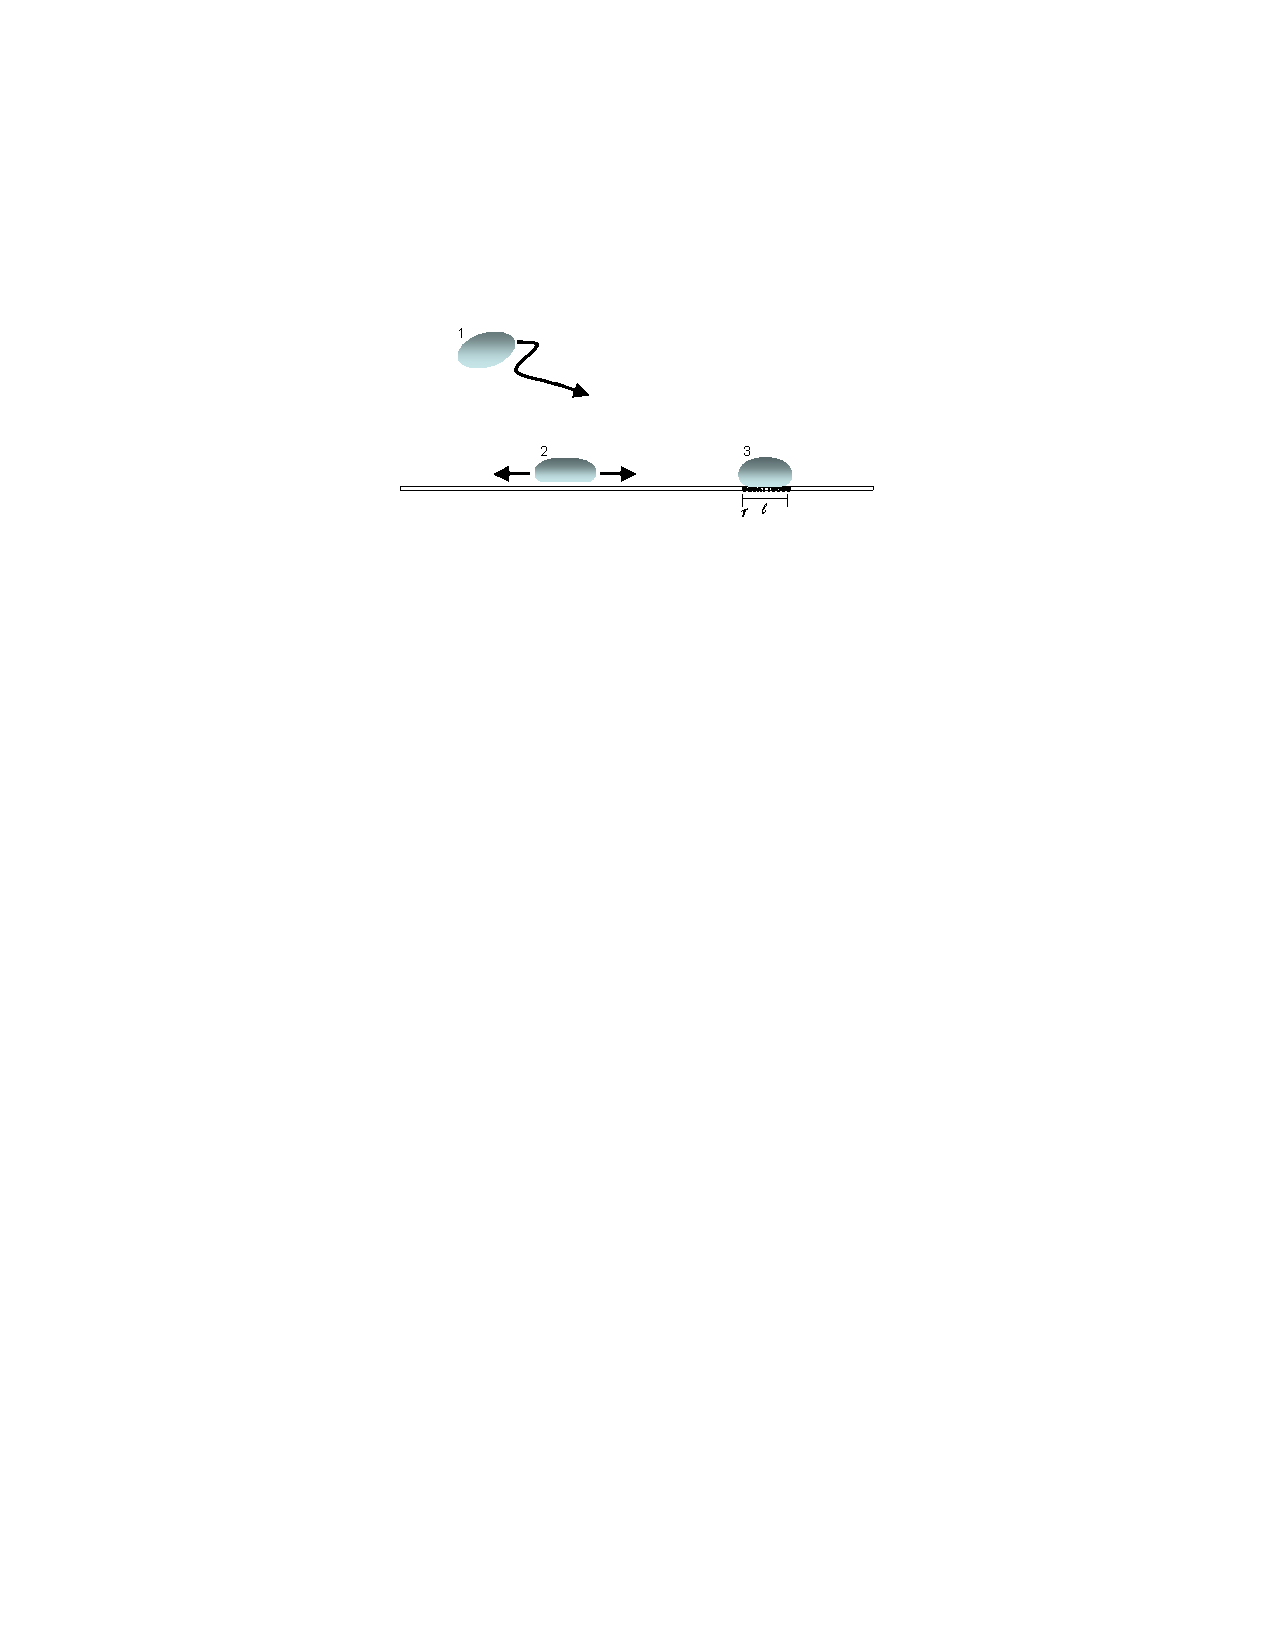
\includegraphics[width=0.8\textwidth]{figures/lassig-TF-search.pdf}
\captionbf{Diff�rents �tats du \tf}{
Figure tir�e de \cite{Lassig2007p539}. Lors de sa recherche de site de
fixation, le TF peut se trouver dans trois �tats distincts : (1) un �tat libre
de diffusion tridimensionnelle, (2) un �tat de diffusion unidimensionnelle sur
l'ADN par fixation non sp�cifique, et (3) un �tat de fixation sp�cifique.
L'�nergie de fixation d�pend du site de fixation, de taille $l$ et de
coordonn�e $r$.
}
\label{fig:lassig-TF-search}
\efig

Un \ft peut �tre dans plusieurs �tats : en diffusion tridimensionnelle, auquel
cas il est dit ``libre'', ou bien fix� sur l'ADN. Dans ce dernier cas, il
interagit avec l'ADN selon deux modes : une attraction non sp�cifique d'�nergie
$E_{ns}$ ind�pendante de la position sur $r$ l'ADN, et une interaction
sp�cifique $E_s(r)$ qui d�pend de la s�quence de taille $l\sim10$ � la position
$r$.  L'interaction non sp�cifique est due � l'interaction �lectrostatique
entre la prot�ine charg�e positivement et l'ADN charg� n�gativement, alors que
l'interaction sp�cifique implique des liaisons hydrog�nes entre le domaine de
fixation de la prot�ine et les nucl�otides du site de fixation. La prot�ine
passe d'un mode � l'autre en changeant de conformation. Au final, le \tf peut
�tre dans trois �tats thermodynamiques repr�sent�s en figure
\ref{fig:lassig-TF-search} : en diffusion tridimensionnelle libre, fix� non
sp�cifiquement (diffusion unidimensionnelle le long de la structure d'ADN), et
fix� sp�cifiquement sur l'ADN. Ces trois modes contribuent � la cin�tique de la
recherche d'un site fonctionnelle \cite{Berg1981kx,Winter1981fk,Winter1981uq}.
Ainsi, l'attraction non sp�cifique conduit la prot�ine � passer � peu pr�s
autant de tant fix� sur l'ADN qu'en diffusion libre. La recherche de site de
reconnaissance est donc un processus mixte de diffusion unidimensionnelle sur
l'ADN et de diffusion tridimensionnelle dans le milieu. Lorsqu'il est fix� sur
l'ADN, le facteur diffuse dans un paysage d'�nergie $E_{ns}$ plat lorsqu'il est
dans sa conformation de fixation non sp�cifique, ou dans un paysage d'�nergie
$E_s(r)$ dans sa conformation de fixation sp�cifique. Cela permet au facteur
d'�chantillonner les sites de faible �nergie $E_s(r)$ tout en �vitant les
barri�res de haute �nergie en passant en mode de recherche non sp�cifique. Ce
processus s'av�re au final tr�s efficace~\cite{Gerland2002p397,Slutsky2004vn}.
Les temps de recherche sont typiquement inf�rieurs � une minute, ce qui est
petit devant les processus de r�gulation de la cellule qui se d�roulent au
mieux sur quelques minutes. Il est donc pertinent de d�crire l'effet d'un site
de fixation sur la r�gulation d'un g�ne cible par la probabilit� qu'il a de
fixer un TF � l'�quilibre thermodynamique.


% subsection modes_de_recherche_du_site_de_fixation_par_le_tf (end)

\subsection{Mod�le PWM} 
Pr�sent� en 1987 par Berg et von Hippel~\cite{Berg1987p3746}, le mod�le PWM est
le mod�le le plus simple d�crivant l'�nergie de fixation sp�cifique entre un \tf et un
site de fixation sur l'ADN.  Ce mod�le repose sur plusieurs hypoth�ses. Tout
d'abord, il y a l'hypoth�se importante que les sites de fixation des TFs sur
l'ADN ont �t� s�lectionn�s au cours de l'�volution pour leur propri�t� de sites
de reconnaissance, qu'elle que soit la concentration du TF dans la cellule. En
d'autres termes, le processus de s�lection discrimine les sites de fixation sur
la seule base de leur �nergie de fixation � un TF donn� : les sites ayant une
�nergie fixation dans une certaine gamme sont retenus, les autres rejet�s.  Par
ailleurs, au sein de cette gamme d'�n�rgie \og utile \fg, toutes les s�quences
sont �quiprobables. Enfin, la derni�re hypoth�se est que chaque nucl�otide d'un
site de fixation contribue de mani�re ind�pendante, \cad additive � l'�nergie
totale du site.  Cette hypoth�se permet de simplifier le probl�me en gardant le
nombre de param�tres petit. L'argument de Berg et von Hippel est que ce
probl�me est analogue � celui de physique statistique consistant � d�duire les
taux d'occupation des niveaux d'�nergie de particules ind�pendantes sachant que
l'�nergie totale doit avoir une certaine valeur moyenne $E$. La solution de ce
probl�me est donn�e par la formule de Boltzmann reliant �nergie et taux
d'occupation :

\begin{equation} 
    f_{i,b} = \exp(-\lambda E_{i,b}) / \Z_i
    \label{eq:boltzmann}
\end{equation}

o� $f_{i,b}$ est la probabilit� d'observer la base $b$ � la position $i$ du
site de fixation, $E_{i,b}$ est l'�nergie associ�e (en $k_BT$), $\Z_i$ est la
fonction partition qui permet de normaliser la distribution � la position $i$,
et $\lambda$ est un facteur sans dimension, analogue du $\beta$ de la
thermodynamique, et li� au processus de s�lection. Dans la suite, nous
int�grerons ce facteur � l'�nergie.  \\ La connaissance des fr�quences des
bases permet de d�finir une autre quantit� utile caract�risant la variabilit�
des s�quences de fixation, l'information relative des sites par rapport � une
s�quence d'ADN al�atoire~\cite{Stormo1998p471}:

\begin{equation} 
    I = \sum_{i=1}^{L}\sum_{b = A,C,G,T}^{}f_{i,b}\ln\left(\frac{f_{i,b}}{\pi_b}\right) 
\end{equation}

o� $L$ est la taille du site de fixation et $\pi_b$ correspond � la probabilit�
\apriori d'observer la base $b$ dans le g�nome. Parce que l'�nergie est d�finie
� une constante pr�s, il est usuel de la d�finir relativement au fond g�nomique
: 

\begin{equation} 
    \tilde{E}_{i,b} = \ln\left(\frac{f_{i,b}}{\pi_b}\right) 
\end{equation}

L'�nergie totale d'un site $S_i$ est alors

\begin{equation}
    \begin{aligned}
        E &= \sum_{i=1}^{L}\tilde{E}_{i,b} \\
        &= \sum_{i=1}^{L}\ln\left(\frac{f_{b(i)}}{\pi_b}\right)\\
        &=\ln\left(\frac{\prod_{i=1}^{L}f_{b(i)}}{\prod_{i=1}^{L}\pi_b}\right)\\
        &=\ln\left(\frac{P(S_i|\text{TF})}{P(S_i|\text{fond g�nomique})}\right)
    \end{aligned}
\end{equation} 

o� $b(i)$ est la base situ�e � la position $i$ du site de fixation. Cette
�nergie quantifie simplement � quel point la s�quence $S_i$ est plus ($E>0$) ou
moins ($E<0$) probablement un site de fixation (de probabilit�
$P(S_i|\text{TF})$) qu'un site tir� au hasard dans le g�nome (de probabilit�
$P(S_i|\text{fond g�nomique})$). On parle aussi de \textit{score} de la
s�quence. L'information relative $I$, qui est le score moyen des s�quences
fix�es par le TF,  peut alors �tre vue comme quantifiant � quel point
l'ensemble des sites de fixation se distingue d'un ensemble de m�me taille de
sites tir�s au hasard.

Avec ces outils en main, il devient alors simple de b�tir un mod�le PWM et de
l'utiliser (fig.~\ref{fig:wasserman-PWM}). �tant donn�s des sites de fixation
connus, il suffit d'�valuer la fr�quence d'occurrence de chaque base � chaque
position. La comparaison avec les probabilit�s g�nomiques \apriori d'occurrence
permet alors de b�tir une matrice score, la PWM. Cette matrice peut alors �tre
utilis�e pour attribuer un score aux s�quences d'ADN en additionnant les scores
� chaque position. Finalement, les s�quences ayant un score d�passant un
certain seuil sont consid�r�es comme des s�quences de fixation.

\bfig
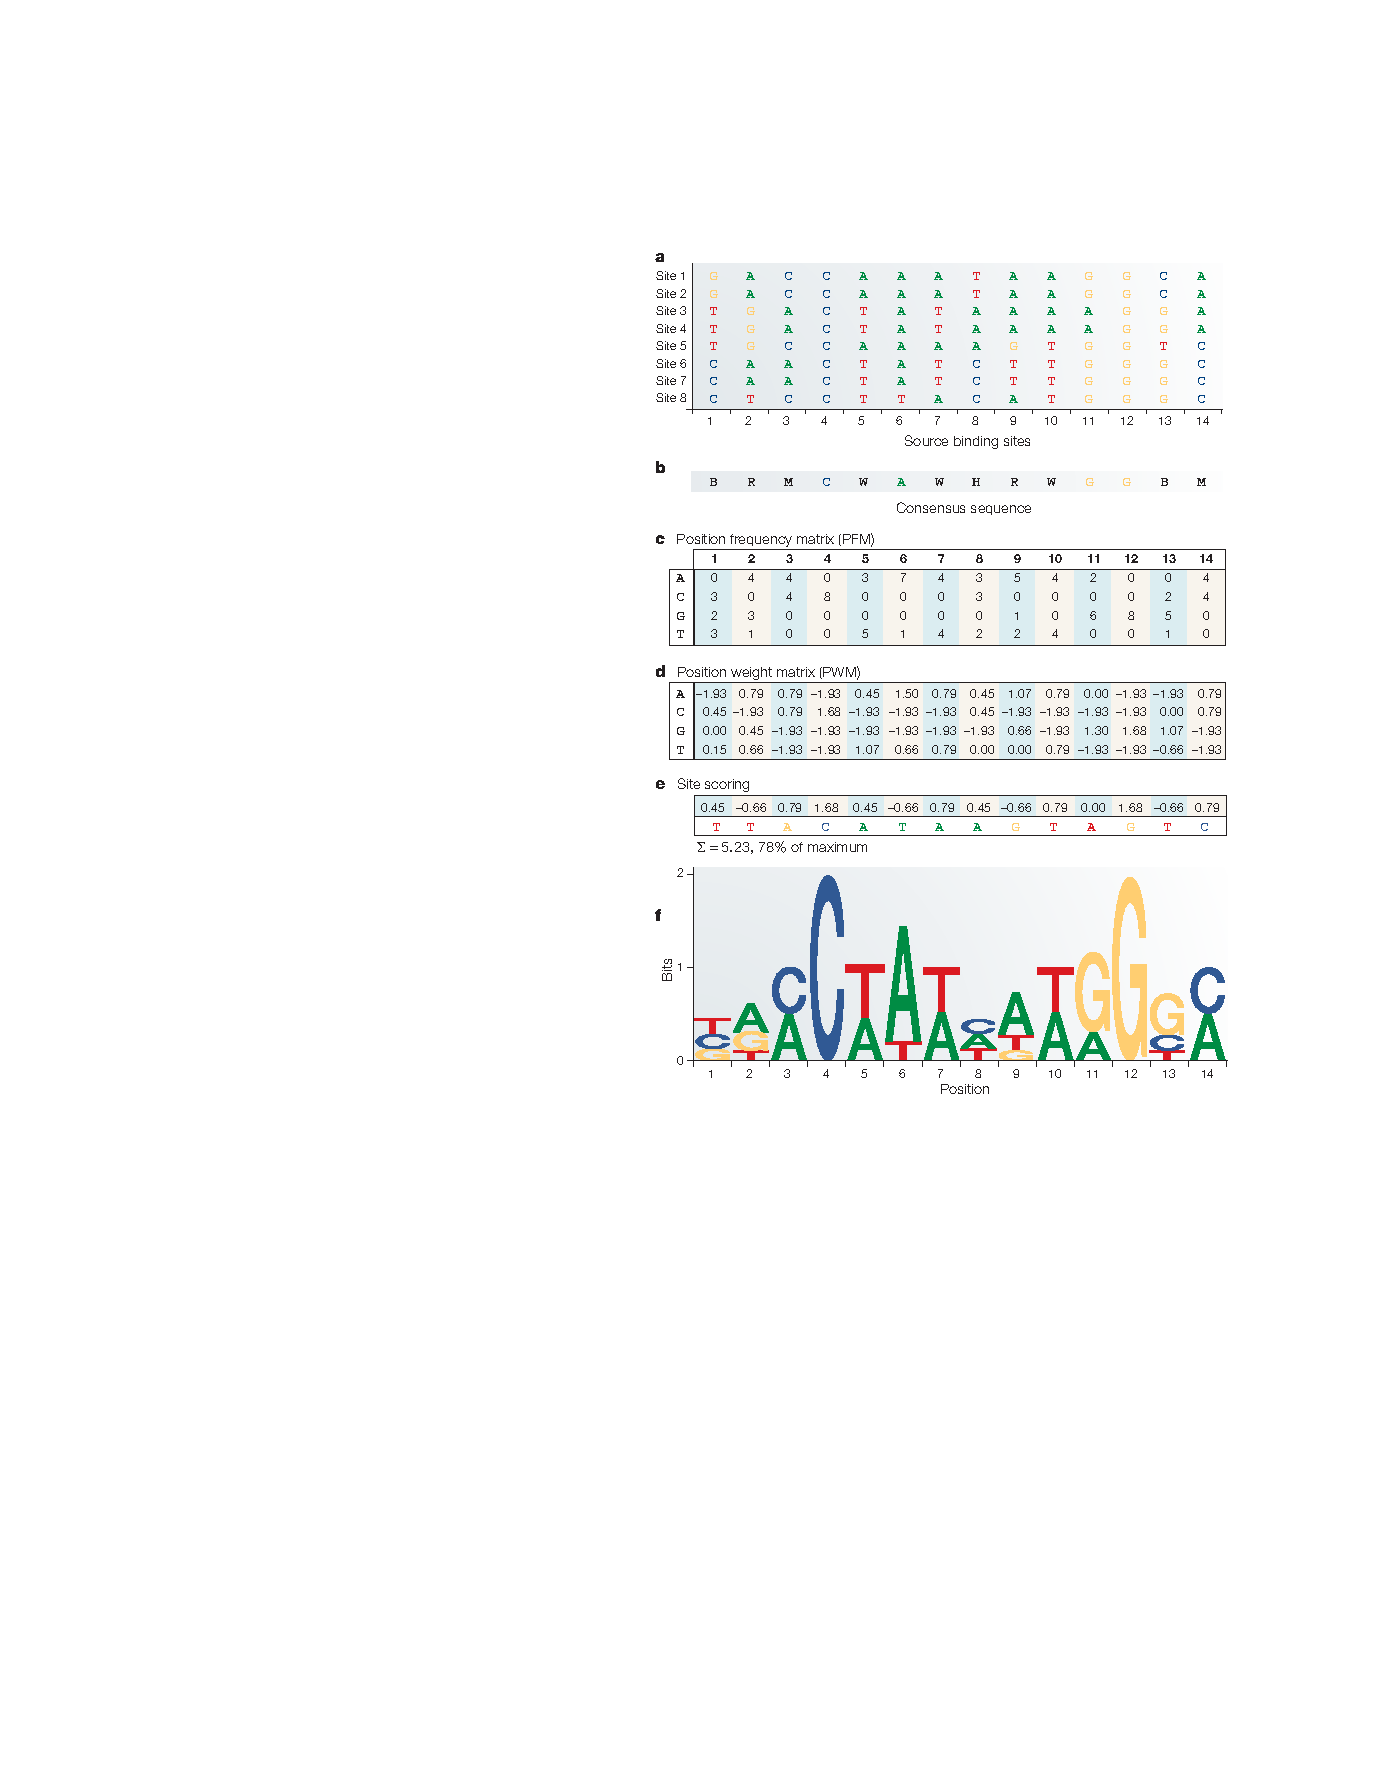
\includegraphics[width=.7\textwidth]{figures/wasserman-PWM.pdf}
\captionbf{Construction et utilisation du mod�le PWM}{
    Figure tir�e de \cite{Wasserman2004p624}. (a) Supposons connus un certain nombre
    de sites de fixation d'un \tf (dans ce cas MEF2).(b) S�quence consensus
    correspondante utilisant les symboles IUPAC. (c) Une matrice de fr�quence
    est construite, indiquant pour chaque nucl�otide sa multiplicit� � une
    position donn�e dans le site. (d) La PWM est simplement construite en
    prenant le logarithme relatif des fr�quences PWMs par rapport aux fr�quences
    \apriori des nucl�otides. (e) Le score (ou �nergie) d'une s�quence d'ADN
    donn�e est calcul� en additionnant les poids PWMs correspondant. (f) La PWM
    peut �tre repr�sent�e sous forme de logo \cite{Giocomo2011p3442}. Dans cette
    repr�sentation, la hauteur d'une colonne repr�sente le contenu en
    information ou information relative moyenne d'une position, et la taille des
    bases refl�te leur fr�quence observ�e.

} 
\label{fig:wasserman-PWM}
\efig

\subsection{Mod�le biophysique}
\label{sub:modele-biophys}

Dans le paragraphe pr�c�dent, nous avons vu que le mod�le PWM est bas� sur une
hypoth�se forte, celle que les sites de fixation ont �t� s�lectionn�s sur la
base de leur seule affinit� ou �nergie envers un TF. N�anmoins, � aucun moment
n'intervient la concentration du TF dans la cellule, dont d�pend pourtant la
probabilit� de fixation. C'est ce que tente de capturer le mod�le
biophysique~\cite{Gerland2002p397,Djordjevic2003p2932,Zhao2009p3948}.  \\

Consid�rons l'interaction entre un TF et une s�quence d'ADN $S_i$ :

\begin{equation}
    TF+S_i \rightleftharpoons TF:S_i
\end{equation}

o� $TF:S_i$ d�note le complexe entre le TF et le site $S_i$. La constante d'�quilibre de cette r�action s'�crit selon la loi d'action de masse :

\begin{equation}
    \label{eq:TF-equilibrium}
    K_i = \frac{[TF:S_i]}{[TF][S_i]}
\end{equation}

Le site peut �tre dans deux �tats : occup� par le TF o� libre. Aussi, la probabilit� que le TF soit fix� au site s'�crit simplement

\begin{equation}
    P(\text{fixation}|S_i) = \frac{[TF:S_i]}{[TF:S_i]+[S_i]}
    = \frac{1}{1+\frac{1}{K_i [TF]}} = \frac{1}{1+\exp(E_i-\mu)}
    \label{eq:modele-biophys}
\end{equation}

o� $E_i=-\ln(K_i)$ est l'�nergie libre standard de fixation (souvent not�e
$\Delta G$), et $\mu=\ln[TF]$ est le potentiel chimique, ces deux quantit�s
�tant exprim�es en $kT$.  Ici nous avons consid�r� qu'il n'y avait qu'un seul
site de fixation. De mani�re g�n�rale, le site est en comp�tition avec le fond
g�nomique, ce qui ajoute une contribution � $\mu$ (voir description
thermodynamique).  � l'instar du mod�le PWM, l'�nergie $E_i$ est g�n�ralement prise comme
�tant une fonction additive des �nergies individuelles des diff�rentes bases du
site. Ainsi, lorsque le TF est � faible concentration ($\mu \to -\infty$), le
mod�le biophysique �crit en �quation~\ref{eq:modele-biophys} se r�duit au
mod�le PWM.


\subsection{Mod�le thermodynamique}

La description biophysique peut �tre r��crite en termes thermodynamiques en
utilisant des raisonnements simples sur le nombre d'�tats possibles et leur
�nergie (et donc poids de Boltzmann) associ�e. Nous adoptons ici l'approche
de~\cite{Gerland2002p397}. On pourra par ailleurs se r�f�rer � l'excellente
revue~\cite{Lassig2007p539}.  Consid�rons le cas simple d'un seul \ft
interagissant avec un g�nome de taille $L \gg 1$ ne contenant qu'un seul site
fonctionnel, le reste de la s�quence �tant al�atoire. La prot�ine se fixe
� l'ADN avec une probabilit� $1/2$.  Lorsqu'elle est fix�e, elle est
� l'�quilibre entre le mode sp�cifique et le mode non sp�cifique. Nous d�sirons
savoir avec quelle probabilit� elle est fix�e de mani�re sp�cifique. La
fonction de partition, �num�rant tous les poids de Boltzmann associ�s aux
diff�rents �tats accessibles au TF fix�, s'�crit :

\begin{equation}
    \Z = \sum\limits_{r=1}^{L} e^{-E_s(r)} + L e^{-E_{ns}}
\end{equation}

o� les �nergies sp�cifique $E_s(r)$ et non sp�cifique $E_{ns}$ sont exprim�es
en unit�s de $k_BT$. Notons $i$ la position du site fonctionnel. On peut �crire :

\begin{equation}
    \begin{aligned}
        \Z & = e^{-E_s(i)} + e^{-E_{ns}} + \sum\limits_{r \neq i} e^{-E_s(r)} + (L - 1) e^{-E_{ns}}\\
    & \simeq e^{-E_i} + \Z_0
\end{aligned}
\end{equation}

o� $Z_0$ est la fonction de partition d'une s�quence al�atoire, et nous avons introduit l'�nergie $E_i$ d�finie par

\begin{equation}
    e^{-E_i} = e^{-E_s(i)} + e^{-E_{ns}}
    \label{eq:Ei}
\end{equation}

Dans le cas d'un site de reconnaissance, $E_s(i) \gg E_{ns}$ de sorte que $E_i
\simeq E_s(i)$~\cite{Gerland2002p397} (ZZ Check ZZ). La probabilit� que le
facteur soit fix� sur le site fonctionnel s'�crit finalement :

\begin{equation}
    P(\text{fixation sp�cifique}|E_i) = \frac{e^{-E_i}}{\Z} = \frac{1}{1+e^{E_i-F_0}}
    \label{eq:fixation-un-tf}
\end{equation}

o� $F_0 = - \log \Z_0$ est l'�nergie libre d'une s�quence g�nomique al�atoire.
On reconnait une fonction de Fermi, avec un seuil d'�nergie � $F_0$ : pour $E_i
< F_0$, la prot�ine est essentiellement fix�e de mani�re sp�cifique � son site
de reconnaissance, alors que pour $E_i > F_0$, elle ne distingue plus le site
du fond g�nomique et y est faiblement fix�e.\\

G�n�ralisons � pr�sent au cas de plusieurs \fts et sites de reconnaissance.
Nous n�gligeons le recouvrement entre \fts fix�s sur des sites proches, qui
poserait des probl�mes st�riques et corr�lerait les sites de fixation dans un
certain voisinage, et consid�rons que le nombre de TFs est grand devant le
nombre de sites de reconnaissance : ainsi, le g�nome est compos� de $L$
s�quences ind�pendantes, chacune pouvant �tre soit non occup�e, soit occup�e de
mani�re non sp�cifique, soit occup�e de mani�re sp�cifique. Notons $\mu$ le
potentiel chimique du TF en solution. La fonction de partition totale est le
produit des fonctions de partition des sites ind�pendants,

\begin{equation}
    \Z(\mu) = \prod\limits_{r=1}^{L}\Z(\mu,r)
\end{equation}

o� la fonction de partition d'un site s'�crit :

\begin{equation}
    \Z(\mu,r) = e^{-\mu} + e^{-E_s(r)} + e^{-E_{ns}}
\end{equation}

En utilisant � nouveau la d�finition de $E_i$ en �q.\ref{eq:Ei}, la probabilit�
de fixation d'un site � la position $i$ s'�crit finalement

\begin{equation}
    P(\text{fixation sp�cifique}|E_i) = \frac{e^{-E_i}}{\Z(\mu,i)} = \frac{1}{1+e^{E_i-\mu}}
\end{equation}

La valeur de $\mu$ est li�e � la fois au nombre de TFs ainsi qu'� la
possibilit� de se fixer dans le fond g�nomique. Elle est bien approxim�e par~\cite{Gerland2002p397}

\begin{equation}
    \mu = F_0 + \log n
\end{equation}

o� $F_0$ est l'�nergie libre du fond g�nomique introduite en
�q.~\ref{eq:fixation-un-tf}. Ainsi, la prise en compte d'une multiplicit� de
TFs ajoute seuil de la fonction de Fermi un facteur $\log n$ par rapport au cas
d'un seul TF. Par ailleurs, cette approche thermodynamique nous a permis de
g�n�raliser le mod�le biophysique simple introduit au paragraphe
\S\ref{sub:modele-biophys}.

\section{Mesures exp�rimentales des interactions prot�ine-ADN}

Ces derni�res ann�es, des avanc�es technologiques consid�rables ont permis
d'une part d'�tablir des mod�les de fixation sp�cifique pour de nombreux TFs,
d'autre part de localiser leurs sites de fixation dans le g�nome. Ces avanc�es
ont eu lieu autant sur le plan \invitro, utilisant prot�ines purifi�es et
s�quences nucl�iques artificielles pour d�duire l'affinit� prot�ine-ADN, que
sur le plan \invivo, mesurant l'interaction de la prot�ine avec l'ADN
g�nomique~\cite{Stormo2010p3947}. 

\subsection{Approches \invitro : MITOMI, SPR, PBM, CSI, SELEX, et HT-SELEX}

\subsubsection{Approche microfluidique : MITOMI}

En 2007, Maerkl et Quake ont mis au point une technique appel�e MITOMI
(Mechanically Induced Trapping Of Molecular Interactions) permettant une mesure
directe de l'affinit� d'un TF � des centaines de s�quences d'ADN � la
fois~\cite{Maerkl2007p840}.  Cette technique repose sur l'utilisation d'un
syst�me microfluidique compos� de chambres dans lesquelles un fluide dont on
peut facilement modifier la composition circule dans des canaux d'un diam�tre
de l'ordre de $1\mu$m dont le microenvironnement est ainsi finement contr�l�.
Dans ce cas, le fluide contient des g�nes synth�tique codant pour le TF ainsi
que du mat�riel permettant la synth�se de la prot�ine au sein de la chambre,
�vitant l'�tape de purification du TF. Chaque chambre du syst�me contient des
anticorps attach�s � la surface permettant de capturer le TF et une certaine
concentration d'une s�quence d'ADN sp�cifique contenant une marque
fluorescente. Le syst�me contient ainsi des centaines de s�quences d'ADN
diff�rentes, chacune �tant pr�sente � diff�rentes concentrations. Lorsque le TF
est fix� par les anticorps, il recrute des s�quences d'ADN selon leur affinit�.
Celles qui ne se fixent pas sont lav�es. Au final, les s�quences fix�es
produisent un signal de fluorescence. La comparaison des signaux pour
diff�rentes concentrations d'ADN donne acc�s au rapport des constantes
d'�quilibre $K_{eq}$ (eq.~\ref{eq:TF-equilibrium}). La comparaison avec une
s�quence r�f�rence dont la constante $K_{eq}$ est connue permet alors de
d�terminer le $K_{eq}$ absolu pour chaque s�quence de fixation.  \\ 

En utilisant $17$ syst�mes de ce type, ils ont ainsi pu mesurer l'affinit� de
$4$ TFs de type bHLH � $464$ s�quences d'ADN diff�rentes: les s�quences
consensus et des s�quences ayant une, deux, trois ou quatre mutations. � titre
de comparaison, ils ont construit une PWM � partir des s�quences contenant une
seule mutation, puis ont pr�dit les �nergies attendues des s�quences
� plusieurs mutations. La pr�diction de la PWM s'est av�r�e bonne dans
seulement $56\%$ des cas pour les s�quences � deux mutations, $10\%$ pour les
s�quences � $3$ mutations et $0\%$ des cas pour les s�quences � $4$ mutations,
montrant les limites de ce mod�le ind�pendant confront� � des donn�es
d'interactions d'ordre sup�rieur. Ainsi, un mod�le plus raffin� prenant en
compte l'�nergie d'interaction non sp�cifique et incluant des interactions
entre nucl�otides voisins permet de rendre compte des valeurs
observ�es~\cite{Stormo2007bh}. Nous reviendrons amplement sur la n�cessit� de
prendre en compte les interactions entre paires de nucl�otides lors de
l'interaction sp�cifique entre TF et ADN dans le chapitre~\ref{ch:maxent}.

\subsubsection{Approche physique : la microscopie SPR}

La m�thode de r�sonance des plasmons de surface (SPR en anglais) est
habituellement utilis�e pour �tudier l'interaction d'une prot�ine avec un
ligand (qui peut �tre une autre prot�ine), mais elle peut aussi �tre utilis�e
pour mesurer les interactions entre une prot�ine et quelques centaines de
s�quences d'ADN diff�rentes~\cite{Shumaker-Parry2004ve,Campbell2007ly}. Le
principe de la microscopie SPR est que l'angle de r�flection de la lumi�re sur
une fine surface d'or, par exemple, d�pend de la masse de mol�cules attach�es
de l'autre c�t� de sa surface. Si de l'ADN est attach� � la surface, la
fixation du TF induit un changement d'angle de reflection lumineuse mesurable
au cours du temps. Ainsi, la cin�tique de fixation du TF jusqu'� l'atteinte de
l'�quilibre est accessible. On peut de m�me �tudier la dissociation du TF lors
du lavage de la surface. Ces mesures donnent directement acc�s aux taux
d'association $k_{on}$ et de dissociation $k_{off}$ que la simple mesure de la
constante d'�quilibre $K_{eq}=k_{on}/k_{off}$ ne permet habituellement pas de
d�terminer.

\subsubsection{Approches bas�es sur des puces � ADN : PBM et CSI}

L'analyse de fixation des prot�ines par puce � ADN (\textit{Protein-Binding
Microarray} ou PBM) est une technologie haut d�bit qui a �t� d�velopp�e au
cours des 10 derni�res ann�es~\cite{Berger2006qf}. Les puces sont compos�es de
$44,000$ puits auxquels sont fix�s des brins d'ADN. Une puce contient tous les
sites de fixation de $10$bp possibles, group�s dans les puits en fonction de
leur coeur de $8$bp ($32,768$ s�quences en comptant les deux brins) avec
possibilit� de distinguer les bases flanquantes dans certains cas sp�cifi�s. Un
TF, purifi� � partir de cellules ou synth�tis� \invitro, est ajout� � la puce,
qui est ensuite lav�e pour se d�barrasser des fixations non sp�cifiques. La
quantit� de prot�ine fix�e � un puits donn� est d�termin�e gr�ce � un anticorps
fluorescent contre la prot�ine. L'enrichissement en prot�ine est calcul�
relativement au bruit de fond (anticorps non sp�cifique par exemple). Il est
alors possible d'utiliser ces mesures pour b�tir une PWM du TF (voir par
exemple~\cite{Kinney2007p3977}).\\

Une autre m�thode utilise aussi des puces � ADN incluant toutes les s�quences
de $10$ bases possibles : c'est l'identification de site apparent�
(\textit{Cognate Site Identifier} ou CSI)~\cite{Warren2006cr}. Une diff�rence
technique avec les PBMs est que l'ADN est d'abord synth�tis� en simple brin
puis se replie en double brin pour former le site de fixation, �vitant ainsi de
devoir g�n�rer l'ADN double brin � partir de pr�curseurs. Par ailleurs, le TF
est en comp�tition avec un marqueur fluorescent qui peut se fixer � l'ADN: il
n'est donc pas n�cessaire d'utiliser un marquage sp�cifique sur le TF ou sur un
anticorps, ce qui rend la proc�dure plus g�n�ralisable. Finalement, la
sp�cificit� du TF est repr�sent�e par un ``paysage de sp�cificit�'' qui
encapsule l'information de fluorescence de l'ensemble des variations par
rapport � une s�quence consensus dans une repr�sentation
simple~\cite{Carlson2010dq}.

\subsubsection{Approche par purification des s�quences fix�es : SELEX et HT-SELEX}

Mise au point il y a plus de $20$ ans, la m�thode SELEX (\textit{Systematic
Evolution of Ligands by EXponential enrichment}) repose sur la s�lection de
s�quences d'ADN al�atoires par un TF
\invitro~\cite{Oliphant1989nx,Tuerk1990qe,Blackwell1990ai,Wright1991dp}. Une
biblioth�que de sites de fixation potentiels est d'abord g�n�r�e en
synth�tisant des s�quences d'ADN al�atoires ou en utilisant des s�quences
g�nomiques. Les bouts de ces s�quences contiennent des pr�curseurs permettant
l'amplification exponentielle par PCR. Le TF purifi� est ajout� aux sites et
les s�quences fix�es sont s�par�es des s�quences non fix�es, par exemple par
retard sur gel. Apr�s un cycle de s�lection, les s�quences r�cup�r�es sont
enrichies en s�quences de basse affinit� pour le TF, car celles-ci sont
simplement initialement bien plus abondantes que les s�quences de haute
affinit�. Afin d'augmenter la proportion de s�quence de grande affinit�, les
s�quences filtr�es sont amplifi�es avant d'�tre filtr�es � nouveau, ceci sur
plusieurs cycles. � la fin de ce processus, les s�quences s�lectionn�es sont
clon�es et s�quenc�es, r�sultant en un nombre typique de moins de $\sim100$
s�quences ind�pendantes~\cite{Fields1997yq}. Si les s�quences initiales sont
issues d'ADN g�nomique, il est possible d'utiliser l'hybridation des s�quences
� des puces � ADN. La pr�sence de plusieurs cycles de s�lection rend n�anmoins
la d�termination des �nergies de fixation moins directe qu'avec les techniques
pr�c�dentes. Une variante de la technique appel�e SELEX-SAGE utilise des
multim�res de sites � la place de sites uniques et permet de r�duire le nombre
de cycles de s�lection et d'augmenter ainsi le nombre de s�quences de fixation
obtenues~\cite{Roulet2002rt}, permettant de r�aliser des mod�les plus
pr�cis~\cite{Nagaraj2008p3749}.

Depuis la m�thode SELEX a �t� mise au point, des avanc�es consid�rables ont �t�
faites dans les techniques de s�quen�age, permettant l'obtention de millions de
s�quences � la fois : on parle de s�quence haut-d�bit
(\textit{high-throughput}) ou encore s�quen�age massivement parall�le.
L'utilisation de ces nouvelles techniques dans l'exp�rience SELEX a men� � la
m�thode HT-SELEX~\cite{Nagaraj2008p3749}, aussi appel�e
Bind-n-Seq~\cite{Zykovich2009gf}. Il est alors possible d'estimer un mod�le
d'�nergie � partir des fr�quences d'observation des diff�rentes s�quences d�s
le premier cycle~\cite{Nagaraj2008p3749}. Des cycles suppl�mentaires permettent
d'obtenir plus d'information sur les s�quences les plus sp�cifiques, notamment
sur la pr�sence de contributions non ind�pendantes � l'�nergie, ou de compenser
la faible sp�cificit� d'un TF. L'avantage de cette technique est que la taille
des sites de fixation n'est pas limit�e. Ainsi, avec une nanomole d'ADN
($\sim10^{15}$ s�quences) on peut couvrir l'ensemble des sites de $25$bp
possibles. Le s�quen�age haut-d�bit permet d'en �chantillonner $\sim10^8$, ce
qui est largement suffisant pour contraindre des mod�les d'�nergie
ind�pendants, m�me pour des TFs ayant des sites de fixations de taille $>15$bp
comme c'est souvent le cas chez la bact�rie. Cette technique a r�cemment �t�
pouss�e encore plus loin~\cite{Jolma2010ul}. En utilisant des prot�ines
marqu�es, les auteurs ont r�alis� un HT-SELEX � partir d'extraits cellulaires,
et en utilisant un code barre aux s�quences d'ADN de chaque exp�rience, ils ont
pu analyser les sites de fixation pour plusieurs TFs en parall�le. Ils ont
r�cemment pu utiliser cette technique pour obtenir des mod�les de sp�cificit�
pour $411$ TFs humains, la plus grande �tude de ce genre r�alis�e � ce
jour~\cite{Jolma2013p3971}.






\subsection{Approche clonale : la technique de simple hybride}
\label{sub:approche_clonale_la_technique_de_simple_hybride}

Contrairement aux approches pr�c�dentes, la technique de simple hybride
(\textit{Bacterial one-hybrid} ou B1H) n'est pas purement \invitro, au sens o�
l'interaction prot�ine-ADN est test�e au sein d'une bact�rie.  N�anmoins, parce
que l'interaction n'est pas test�e dans son contexte cellulaire d'origine, nous
la consid�rerons comme telle. Cette approche repose sur l'int�gration par une
bact�rie h�te de deux vecteurs d'expression g�n�tique, ou plasmides. Le premier
exprime le \tf d'int�r�t fusionn� � une sous-unit� de l'ARN polym�rase
(l'app�t), c'est la prot�ine ``hybride''. L'autre contient une r�gion de
s�quence al�atoire repr�sentant un site de fixation potentiel (la proie) en
amont d'un promoteur � faible activit�. La fixation de cette r�gion par la
prot�ine hybride permet l'activation d'un g�ne de s�lection, g�n�ralement
\textit{HIS3}, un g�ne de la levure requis pour la biosynth�se de l'histidine
et dont l'homologue bact�rien est absent de la souche d'\ecoli utilis�e. La
croissance des cellules a lieu dans un milieu ne contenant pas l'histidine.
Dans ces conditions, les bact�ries n'exprimant pas \textit{HIS3} ne peuvent
cro�tre. Ainsi, seules les bact�ries dans lesquelles le \tf se fixe � la proie
expriment \textit{HIS3}, croissent et forment des colonies, d'o� la notion de
g�ne de s�lection. Par ailleurs, la stringence de la s�lection peut �tre
modul�e en ajoutant au milieu diff�rentes concentrations de 3-amino-triazole
(3-AT), un inhibiteur de \textit{HIS3}. De cette fa�on l'affinit� du site de
fixation peut �tre estim�e plus finement.  
\\ 

Dans les �tudes de ce type, les sites de fixation pr�sents au sein des colonies
sont s�quenc�s individuellement, ce qui permet d'obtenir environ $50$ s�quences
pour une exp�rience de s�lection donn�e~\cite{}. N�anmoins, il semble possible
d'utiliser les nouvelles technologies de s�quen�age pour r�cup�rer l'ensemble
des sites de fixation des bact�ries pr�sentes sur une
plaque~\cite{Stormo2010p3947}.  � l'instar de la m�thode HT-SELEX, on obtient
des millions de sites, ceux ayant une plus grande affinit� �tant pr�sents
� plusieurs centaines de milliers d'exemplaires, et ceux ayant une faible
affinit� �tant pr�sent en un seul voire aucun exemplaire.
\\

Notons qu'il est aussi possible d'adopter la d�marche inverse, \cad de partir
de quelques sites de fixation pr�sum�s fonctionnels mais pour lesquels on ne
conna�t pas le TF associ�. En utilisant une biblioth�que de plasmides codant
pour diff�rents TFs hybrides, il est alors possible de d�terminer si l'un
d'entre eux poss�de une affinit� importante avec les sites test�s.

% subsection approche_clonale_la_technique_de_simple_hybride (end)
\subsection{Approches \invivo : \chipchip, \chipseq, DNAse I}

Dans cette section, nous nous int�ressons aux techniques permettant
d'identifier les sites de fixation d'un \tf sur le g�nome. Ces m�thodes se
basent sur des extraits cellulaires (de $10^4$ � $10^8$ cellules) qui peuvent
provenir d'un tissu homog�ne (un seul type de cellule) ou h�t�rog�ne (plusieurs
types de cellules), voire de l'organisme entier si la dissection est impossible
(embryon de mouche par exemple). L'information obtenue est donc toujours
conditionn�e par ce mat�riau de d�part, et l'on n'obtient que les sites
\textit{accessibles} �tant donn�es le type cellulaire et la p�riode de
d�veloppement �tudi�s.

\subsubsection{Immunopr�cipitation de la chromatine : \chipchip et \chipseq}

\bfig
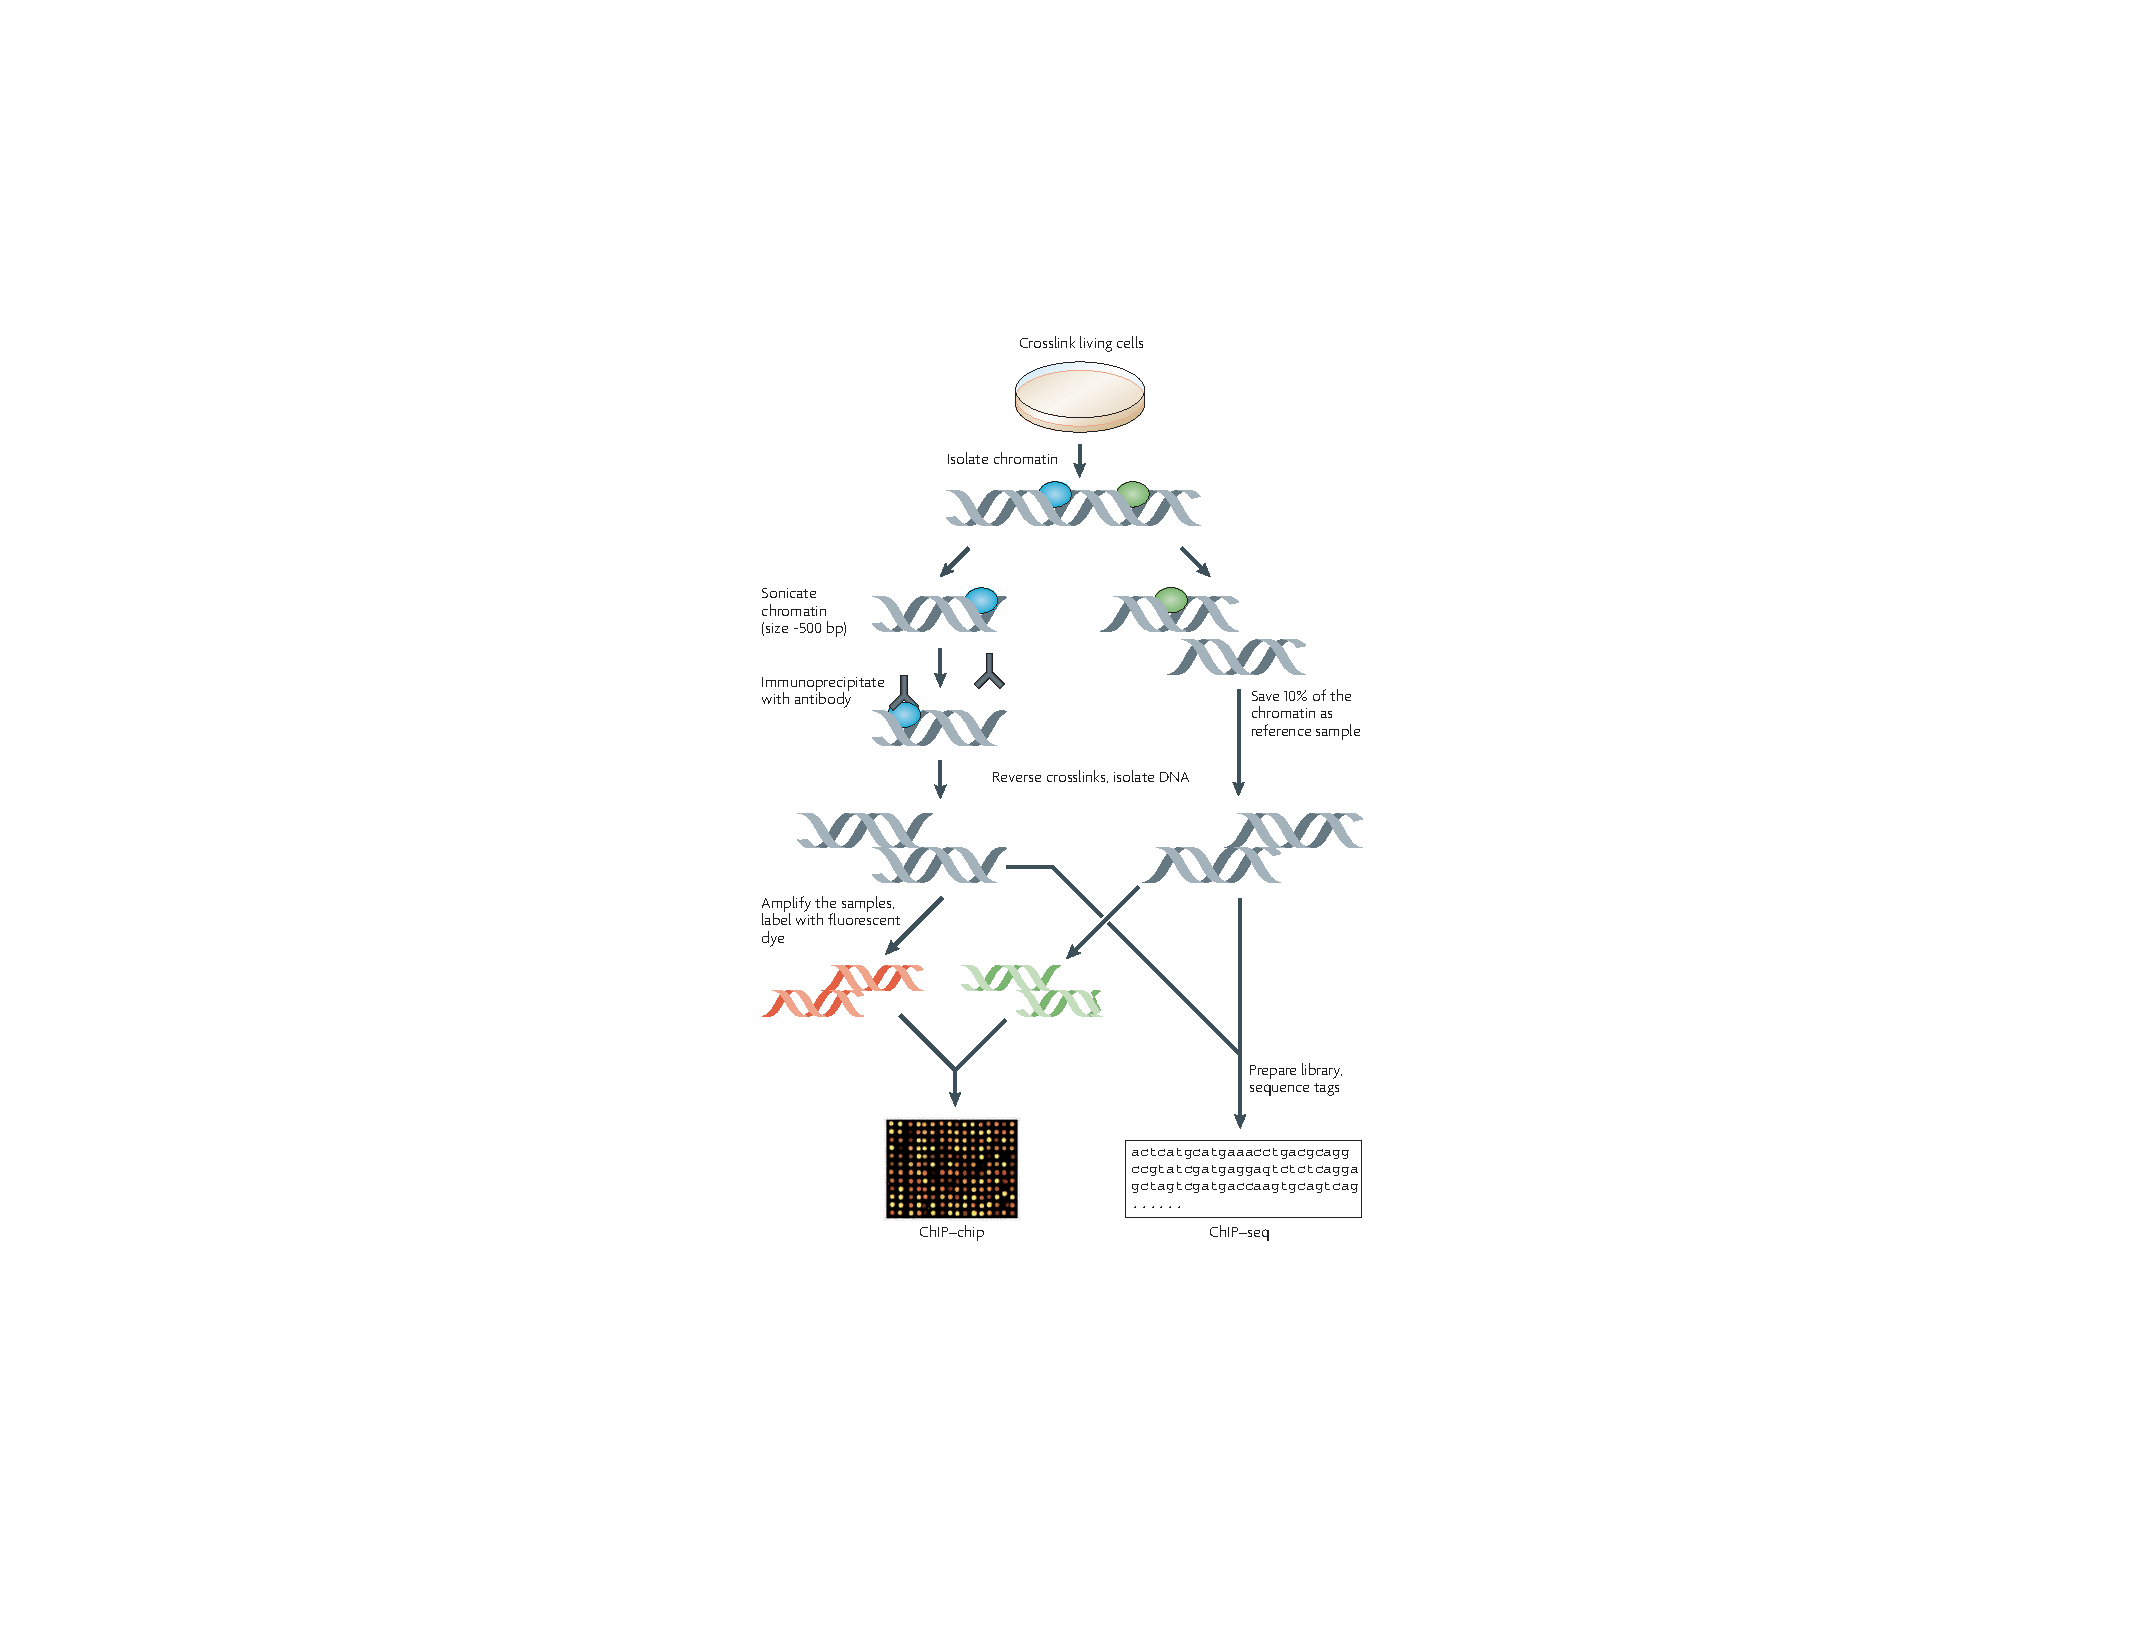
\includegraphics[width=0.8\textwidth]{figures/farnham-chip.pdf}
\captionbf{�tapes d'une exp�rience de \chipseq}{
    Figure tir�e de \cite{Farnham2009fk}.
}
\label{fig:farnham-chip}
\efig


La technique d'immunopr�cipitation de la chromatine (ChIP)
(fig.~\ref{fig:farnham-chip}) consiste dans un premier temps � induire la
r�ticulation (\textit{crosslink}) des prot�ines se liant � l'ADN avec l'ADN en
traitant les cellules avec de la formald�hyde. Cette �tape permet de
transformer les liaisons faibles prot�ine-ADN en liaisons covalentes. Une fois
les prot�ines fix�es, la chromatine est d�coup�e par digestion enzymatique ou
en la soumettant � des ultrasons (c'est la sonication), r�sultant en des
fragments de taille variant entre $200$ et $600$bp. Ces fragments sont ensuite
immunopr�cipit�s en pr�sence d'un anticorps sp�cifique d'un \tf ou d'un isoforme
d'histone (dans le cas d'une �tude du paysage �pig�n�tique) d'int�r�t, permettant ainsi de r�cup�rer tous les sites de fixation dans le g�nome. Apr�s purification des fragments pr�cipit�s, l'�chantillon peut �tre analys� soit par hybridation sur puce (\chip) ou par s�quen�age haut d�bit (\chipseq).\\

Dans le cas de la \chipchip, l'�chantillon immunopr�cipit� et l'ADN de d�part
(\textit{input}) sont marqu�s avec des colorants fluorescents et hybdrid�s
� une puce � ADN compos�e de tr�s nombreux puits contenant des
oligonucl�otides (courtes s�quences d'ADN) correspondant � diff�rentes r�gions
du g�nome. Dans le meilleur cas, ces oligonucl�otides couvrent l'ensemble du
g�nome. Les sites de liaison sont identifi�s par l'�cart d'intensit� entre les
signaux de fluorescence des conditions d'immunopr�cipitation et
d'\textit{input}.
\\

\bfig
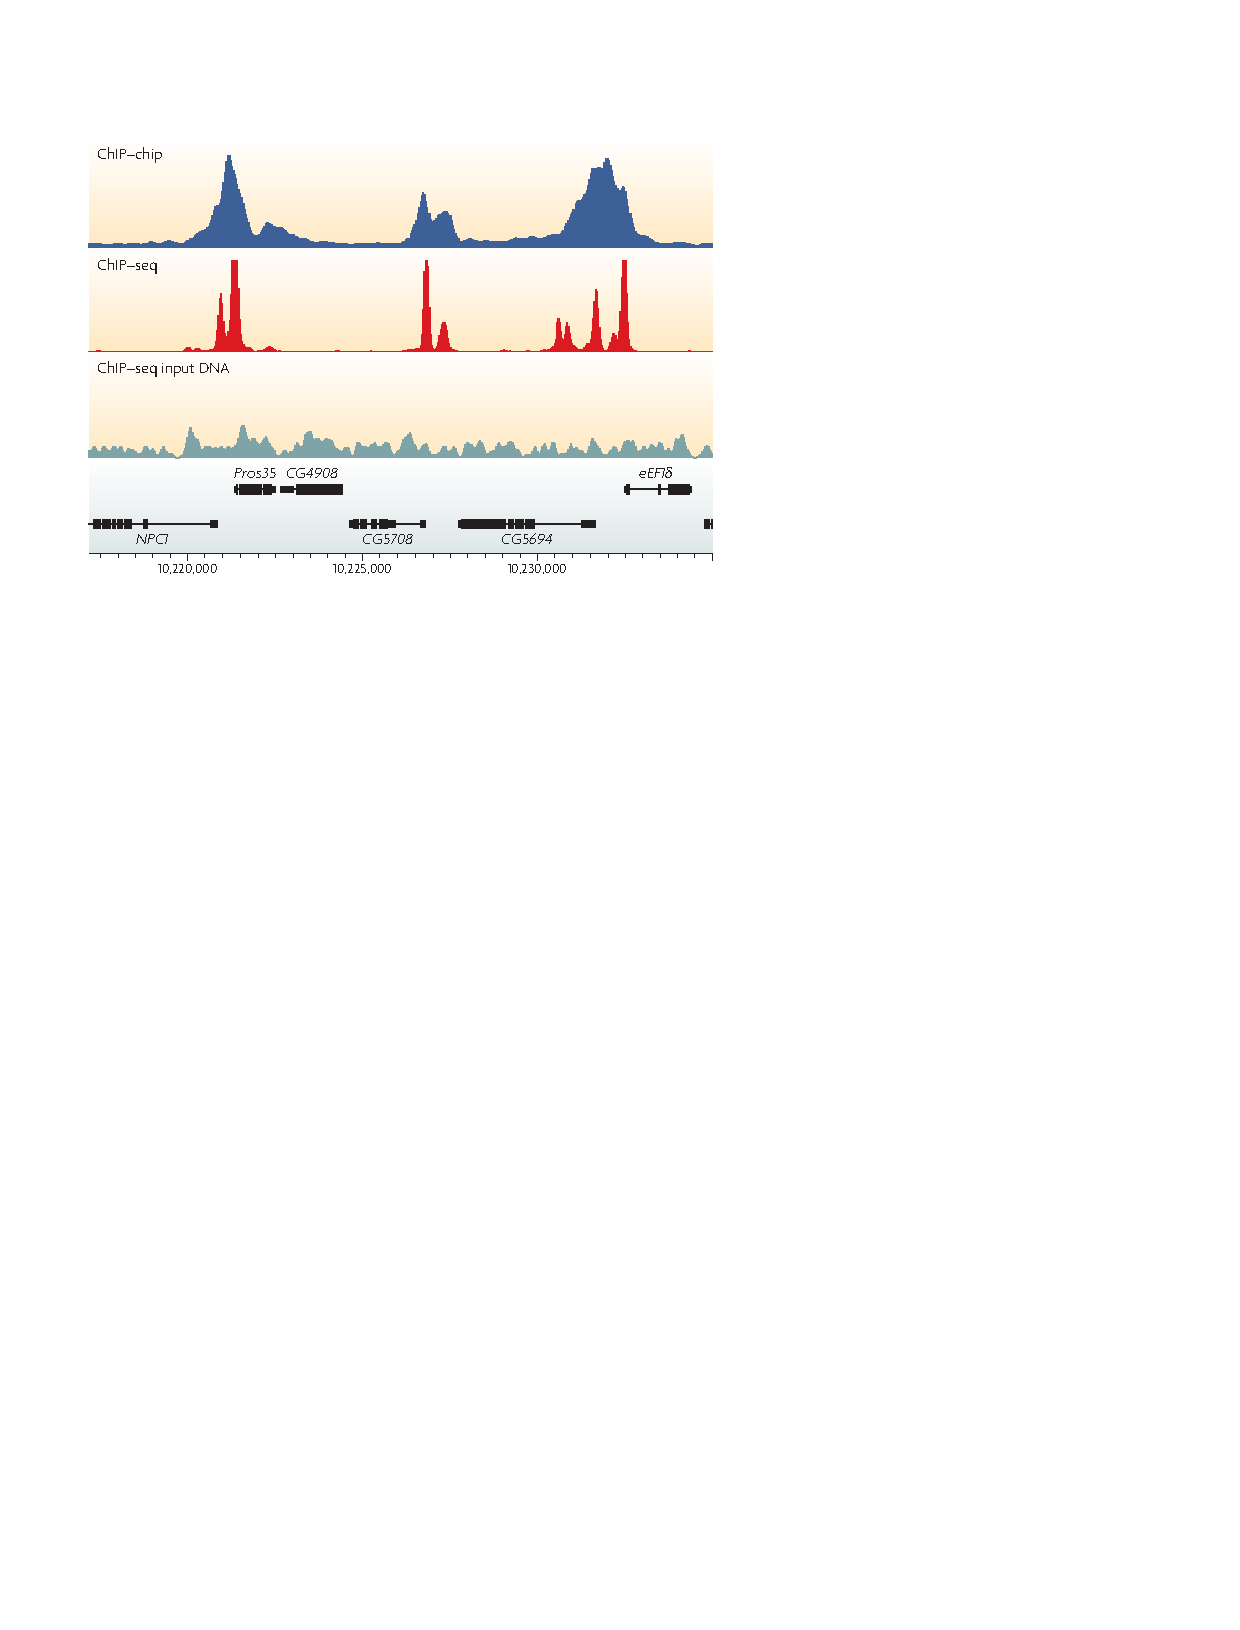
\includegraphics[width=0.6\textwidth]{figures/park-chip-resolution.pdf}
\captionbf{R�solution des exp�riences \chipchip et \chipseq}{
Figure tir�e de \cite{Park2009kx}. Exemples de profils de fixation de la
prot�ine � chromodomaine Chromator g�n�r�s � partir d'exp�riences de \chipchip
(intensit� relative par rapport au contr�le, bleu) et de \chipseq (densit� de
s�quences, rouge) dans la lign�e cellulaire S2 de \dmel. On peut noter la plus
grande r�solution de l'exp�rience \chipseq pour d�terminer les sites de
liaison. L'ADN utilis� en \textit{input} de l'exp�rience de \chipseq et servant
de contr�le est montr� en gris.
}
\label{fig:park-chip-resolution}
\efig

Dans le cas du \chipseq, l'�chantillon immunopr�cipit� est analys� par
s�quen�age � haut d�bit, r�sultant en une librairie de \textit{reads} d'une
longueur typique variant entre $27$ et $50$bp issus des bouts des s�quences.
Ces \textit{reads} sont ensuite align�s sur un g�nome de r�f�rence. � chaque
position du g�nome correspond ainsi un certain nombre de s�quences pr�cipit�es
et d'\textit{input}. En comparant ce nombre au nombre moyen dans le locus et
� l'\textit{input}, il est possible d'identifier des pics correspondant � la
fixation du facteur (voir par exemple le programme d'appel de pics \chipseq
MACS \cite{Zhang2008uq}).  \\

Dans les deux cas, il faut noter que l'on a affaire � la fixation
\textit{moyenne} du facteur sur l'ADN dans la population de cellules �tudi�e.
Ainsi, un petit pic peut repr�senter aussi bien une fixation forte dans un
petit sous-ensemble de cellules (par exemple celles qui sont � un certain �tat
d'avancement du cycle cellulaire) qu'une fixation moyenne dans l'ensemble de la
population. L'exp�rience de \chipseq offre une r�solution bien plus pr�cise
($\leq100$nt) que la m�thode \chipchip (fig.~\ref{fig:park-chip-resolution}).
En effet, dans ce dernier cas la r�solution est limit�e par le nombre
d'oligonucl�otides utilis�s, qui sont dans le meilleur des cas r�partis sur le
g�nome avec $35-100$ nucl�otides d'�cart entre deux instances. Pour se comparer
� la \chipseq, il faudrait que tous les oligonucl�otides se superposent � une
base pr�s, ce qui demanderait un trop grand nombre de puces.


\subsubsection{Empreinte � la DNase I (\textit{DNase I footprinting})}

\bfig
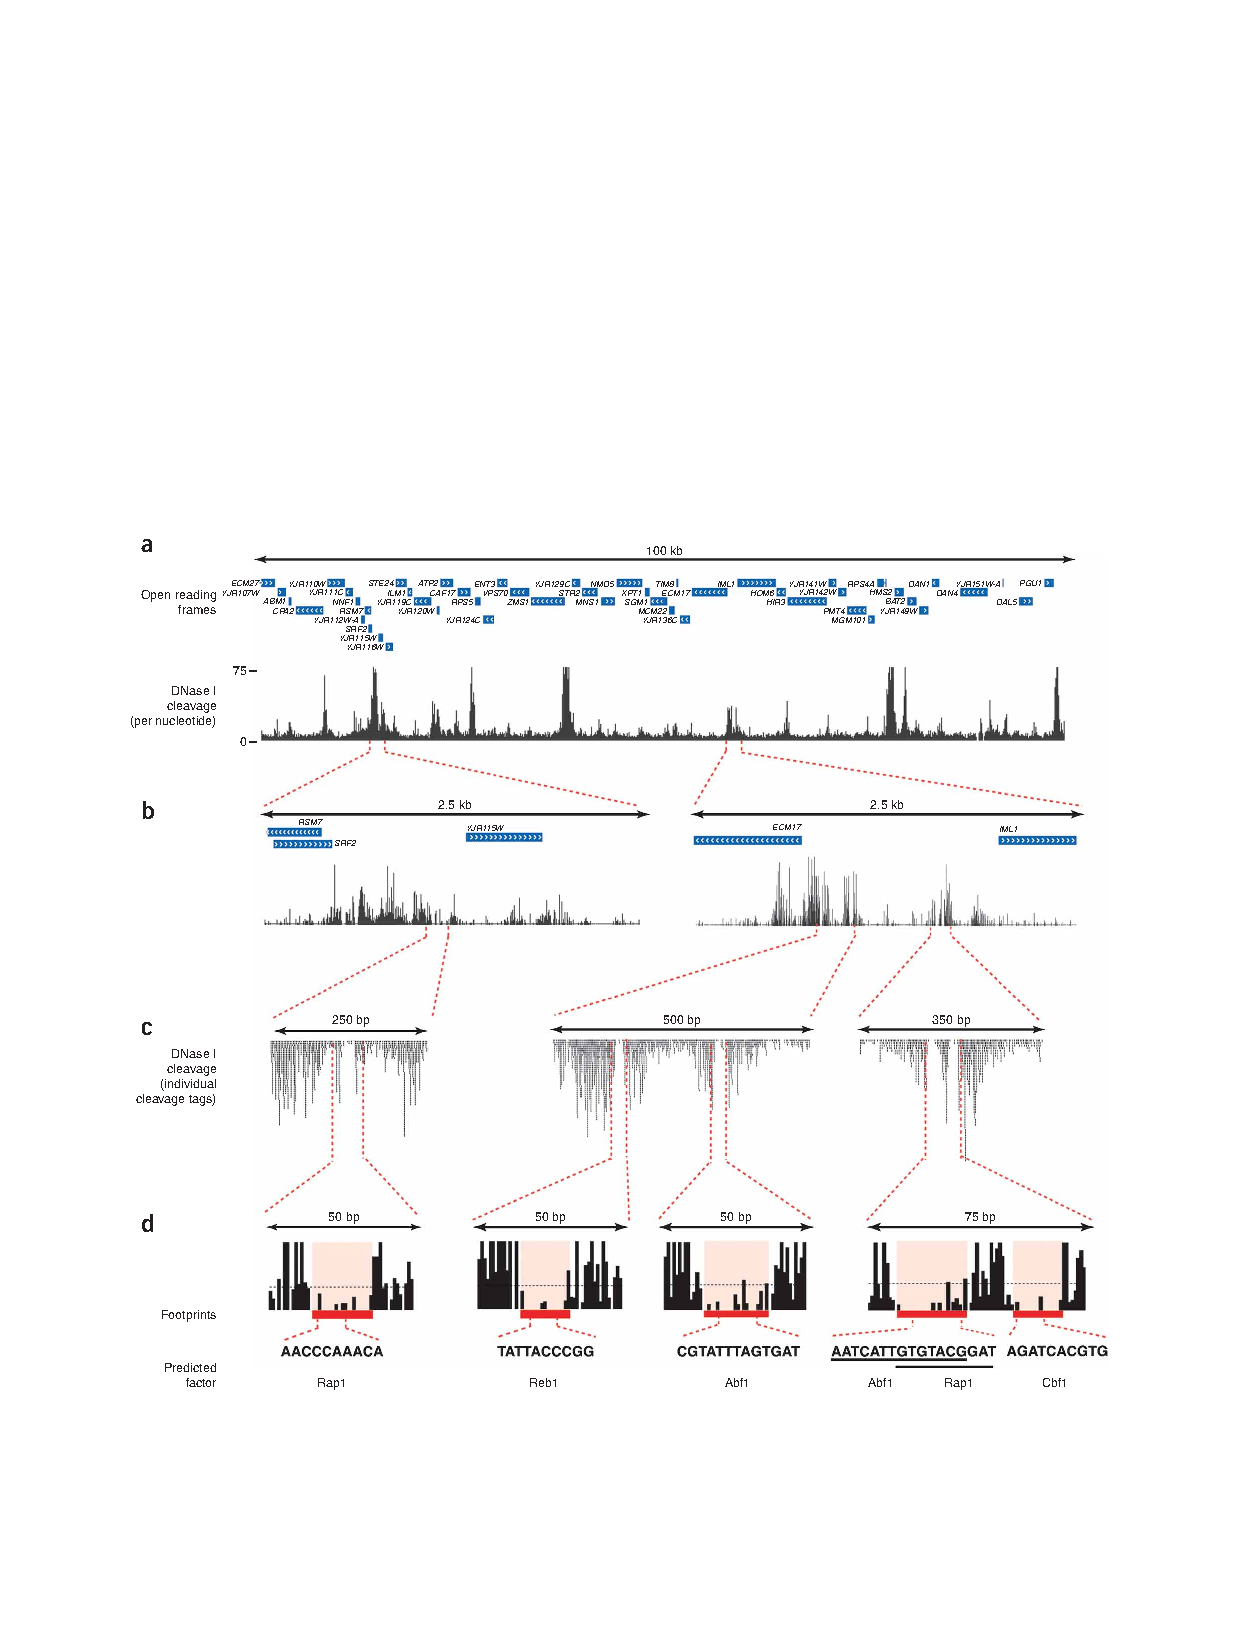
\includegraphics[width=\textwidth]{figures/hesselberth-dnase.pdf}
\captionbf{Exp�rience d'empreinte � la DNase I chez la levure : vers une r�solution au nucl�otide pr�s}{
Figure tir�e de \cite{Hesselberth2009vn}. (a) Densit� de digestion de la DNase
I par nucl�otide dans une r�gion de $100$kb du g�nome de la levure contenant
$\sim50$ g�nes (bo�tes bleues). On voit clairement certaines r�gions
promotrices marqu�es par la DNase I. (b) Zoom sur deux r�gions de $2.5$kb. (c)
Zoom sur des r�gions de $250$bp. Le nombre d'�v�nements de digestion par
nucl�otide est marqu� par des empilements de bo�tes noires, r�v�lant des
r�gions prot�g�es : ce sont les empreintes � la DNase I. (d) Les empreintes
sont associ�es � des motifs de r�gulation de la levure connus. Les pointill�s
noirs indiquent le nombre moyen de digestion par nucl�otide dans le g�nome
($\sim2$ digestions par base).
}
\label{fig:hesselberth-dnase}
\efig

Contrairement aux techniques pr�c�dentes, l'empreinte � la DNase I ne repose
pas sur l'�tude d'un \tf pr�cis, mais permet au contraire d'avoir un ensemble
de sites de fixation dans le g�nome pour un type cellulaire donn�, avec une
pr�cision au nucl�otide pr�s. Cette m�thode repose sur le fait que la fixation
stable des \tfs � l'ADN n'est possible que si la r�gion est pauvre en
nucl�osomes, les prot�ines autour desquelles s'enroule l'ADN : on parle de
r�gion de chromatine ouverte. Ces r�gions sont pr�f�rentiellement dig�r�es par
l'endonucl�ase DNase I. �tant donn� que la majorit� de l'ADN est enroul� autour
de nucl�osomes, les sites hypersensibles � la digestion par DNase
I (\textit{DNase I-hypersensitive} ou DHS) correspondent essentiellement � des
r�gions de chromatine ouverte ayant des roles de r�gulation g�n�tique
: promoteurs, enhancers\ldots 
\\

En combinant la technique de DHS avec le s�quen�age � haut d�bit, l'exp�rience
de DNase-seq permet d'identifier tous les types de r�gion de r�gulation
� l'�chelle du g�nome~\cite{Thurman2012ys}. Les r�gions riches en sites de digestion
identifient alors les sites DHS. Par ailleurs, au sein d'un site DHS, il y a de
petites r�gions ($\sim15$bp) qui sont prot�g�es de la digestion par DNase
I : ce sont les empreintes � la DNase I ou \textit{DNase I footprints}
(fig.~\ref{fig:hesselberth-dnase}). Ces empreintes sont dues � la pr�sence de
prot�ines ou de complexes fix�s � l'ADN. Cette technique de d�tection de sites
de liaison par empreinte � la DNase I existe depuis $30$ ans mais n'a que
r�cemment �t� port� � l'�chelle g�nomique. En comparant � des donn�es \chipseq
ou en utilisant des bases de donn�es de motifs de \tfs, il est possible
d'identifier le facteur correspondant dont les sites de fixation sont alors
connus au nucl�otide pr�s.



\section{Les modules de cis-r�gulation} \label{sec:CRMs} 
%
%\begin{malistebullet}{15}
%\item R�gulation transcriptionnelle. Facteurs de transcription. Diffusion, fixation. \\
%\item   Mod�les math�matiques (PWM, biophysiques). \\
%\item   Coop�rativit�, fonctions logiques, coefficients de Hill (Uri Alon).\\
%\item   Donn�es biologiques grande �chelle : \chipseq etc\ldots Bioinformatique.\\
%\item   ENCODE, Taipale, etc.\\
%\item   Evolution de la r�gulation Odom, Sinha.\\
%\end{malistebullet}

Nous l'avons vu en \ref{sub:divers_modes_de_regulation}, les s�quences d'ADN
r�gulant l'expression g�n�tique -- CRMs pour \textit{Cis-Regulatory Modules} --
jouent un r�le pr�pond�rant au cours du d�veloppement des organismes. Ces CRMs
assurent en effet l'orchestration de l'expression de g�nes sp�cifiques aux
diff�rentes �tapes du d�veloppement et aux divers types cellulaires. Ils sont
au coeur de l'�volution des r�seaux g�n�tiques, car ils dictent les
interactions entre g�nes. De plus, leur alt�ration peut �tre au coeur de
nombreuses pathologies, li�es pour la plupart � une expression g�n�tique
aberrante. Par exemple, la majeure partie des variants g�n�tiques qui sont
associ�s de mani�re significative � une susceptibilit� envers une maladie sont
situ�s hors des r�gions codant pour des prot�ines, sugg�rant qu'un certain
nombre affectent non pas la forme de la prot�ine engendr�e mais l'expression du
g�ne la produisant en d�truisant une activit� CRM. Dans cette partie, nous
proposons un survol des diff�rents types de CRMs, de leur structure, leur
�volution et leur pr�diction.

\subsection{Les diff�rents types de CRMs}
\label{sub:les_diff_rents_types_de_crms}

\bfig
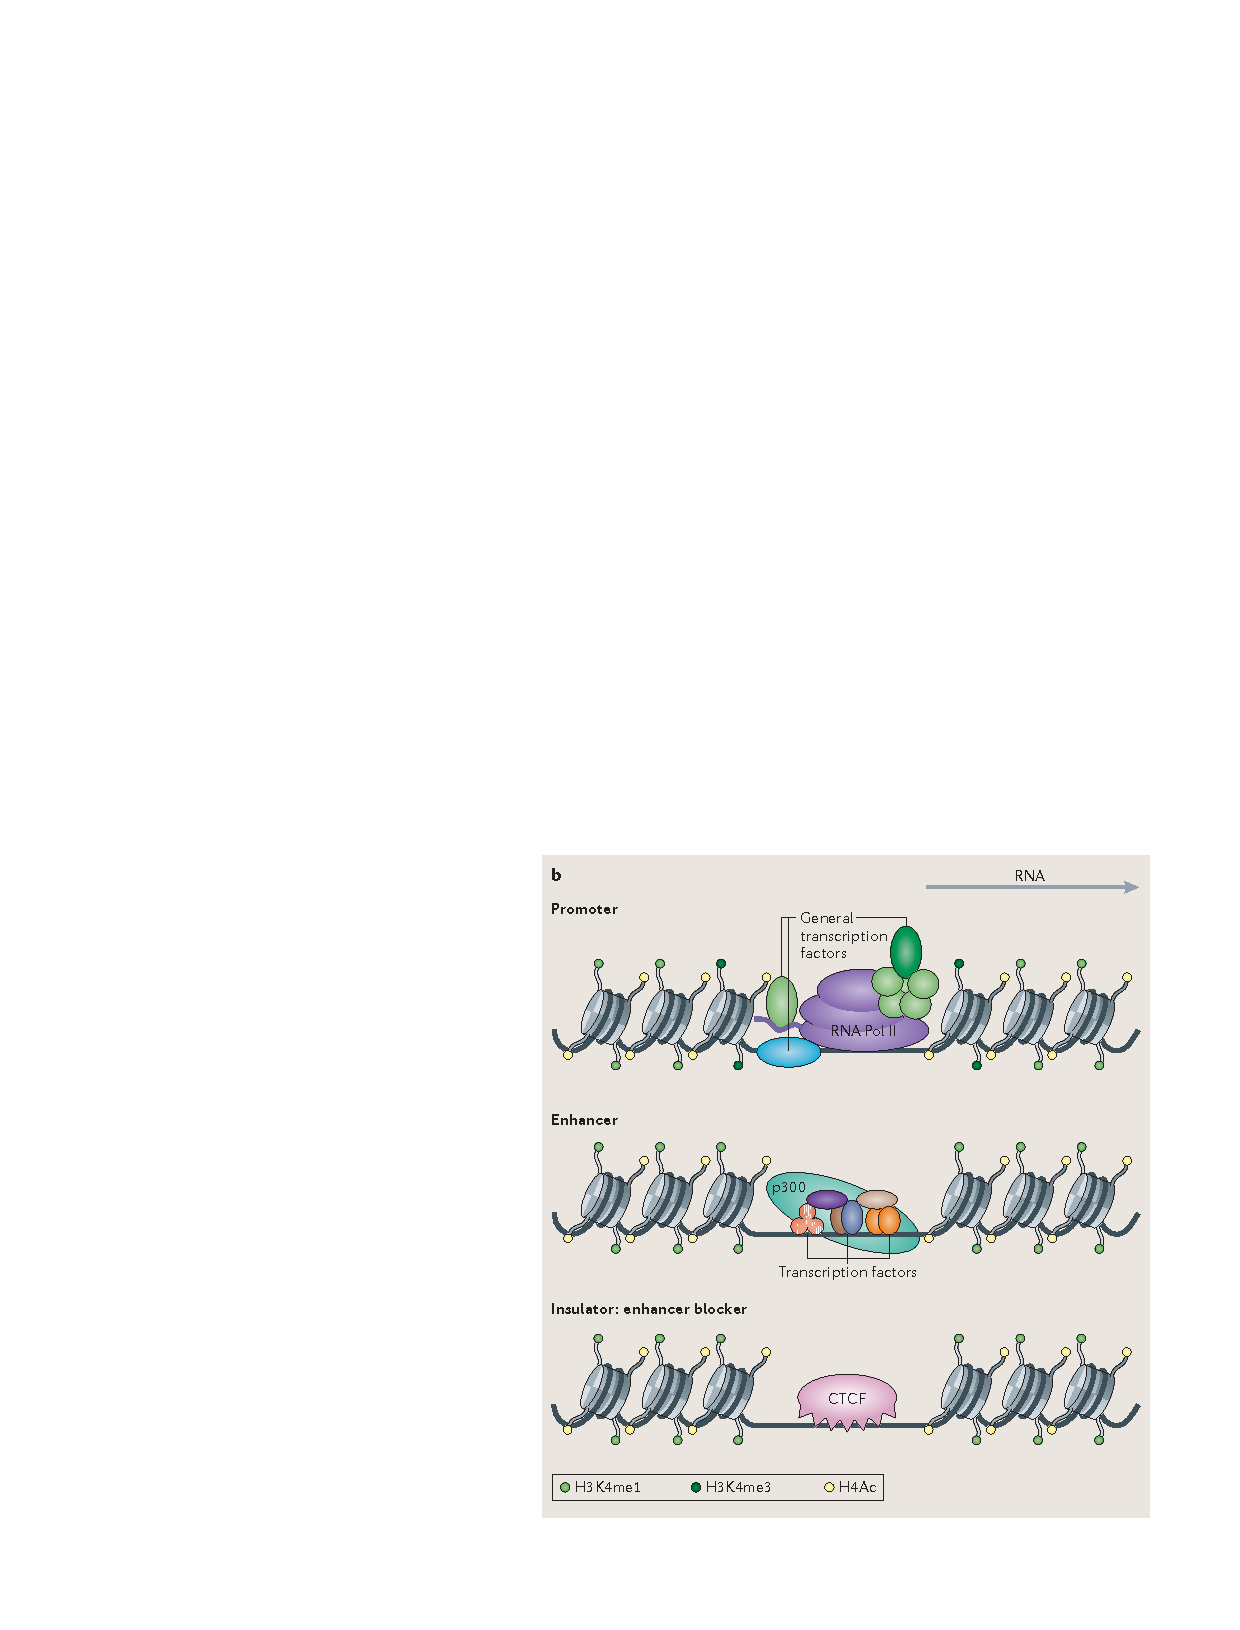
\includegraphics[width=.8\textwidth]{figures/hardison-enhancer-states.pdf}
\captionbf{Les diff�rents types de CRMs et leurs marques �pig�n�tiques} 
{ 
    
    Figure tir�e de \cite{Hardison2012p3778}. La notion de CRM renvoie � un
    regroupement de sites de liaison pour un ou plusieurs \fts. Les CRMs
    peuvent �tre regroup�s en plusieurs classes : les promoteurs, les
    \textit{enhancers}/\textit{silencers}, et les insulateurs. Les CRMs des
    diff�rentes classes partagent les marques d'ac�tylation H3Ac et H4Ac, les
    promoteurs actifs sont sp�cifiquement marqu�s par H3K4me$3$, et les enhancers
    et insulateurs sont marqu�s par H3K4me$1$. Les enhancers sont par ailleiurs souvent
    fix�s par le co-activateur p300. Enfin, chez les mammif�res les insulateurs
    recrutent CTCF pour bloquer l'activation par les enhancers.

} 
\label{fig:hardison-enhancer-states}
\efig

La r�gulation de l'expression g�n�tique implique l'interaction entre des \fts
et des CRMs. Selon leur r�le dans la r�gulation de l'expression g�n�tique, les
CRMs peuvent �tre distingu�s en trois cat�gories.

\subsubsection{Promoteurs}
\label{ssub:promoteurs}

Les promoteurs permettent la fixation de l'ARN polym�rase pour d�buter la
formation d'un transcrit ARN au site d'initiation de transcription
(\textit{Transcription Start Site} ou TSS). Dans les promoteurs fixant l'ARN
polym�rase II (la majorit� des promoteurs eucaryotes), des \fts g�n�raux se
fixent � un coeur de $\sim100$bp autour du TSS afin de faciliter la fixation du
complexe de polym�rase. Ces coeurs de promoteurs contiennent pour certains des
motifs st�r�otyp�s, comme la bo�te TATA, et on un TSS bien d�termin�; n�anmoins
la plupart des promoteurs des g�nomes mammif�res sont des r�gions riches en GC
et en dinucl�toides CpG (les \og �lots CpG \fg) qui ne poss�dent pas de bo�te
TATA et permettent l'initiation de la transcription dans un interval d'environ
$100$ bases~\cite{Carninci2006qf}. Au niveau �pig�n�tique, les promoteurs
actifs poss�dent une r�gion pauvre en nucl�osomes en amont du TSS, flanqu�e de
nucl�osomes poss�dant la marque de m�thylation H3K4me3.

% subsubsection promoteurs (end)

\subsubsection{\textit{Enhancers} et \textit{silencers}}
\label{ssub:enhancers_et_silencers}

Les \textit{enhancers} et \textit{silencers} sont respectivement d�finis par
leur effet positif ou n�gatif sur l'expression d'un g�ne cible. Cet effet peut
notamment �tre observ� par transfert d'un plasmide contenant l'�l�ment
r�gulateur en amont d'un g�ne rapporteur dans un animal transg�nique ou dans
des cultures cellulaires transfect�es (voir
\ref{sub:validation_experimentale}). Leur activit� ne d�pend g�n�ralement pas
de leur position et de leur orientation sur le plasmide. Selon l'environnement
cellulaire, une r�gion r�gulatrice peut �tre soit \textit{enhancer} soit
\textit{silencer}, en fonction de la nature de co-activateurs ou de
co-r�presseurs des TFs recrut�s. Il y a n�anmoins relativement peu de
\textit{silencers} caract�ris�s et l'on utilise le terme d'\textit{enhancers}
pour d�signer de mani�re g�n�rale ces r�gions r�gulatrices.

Les \textit{enhancers} peuvent se situer � des distances variables du g�ne
qu'ils r�gulent~\cite{Maniatis1987fk}, pouvant parfois aller jusqu'� $1$ Mb
comme dans le cas de \textit{Shh} chez la souris~\cite{Lettice2003uq}. Les
enhancers contiennent de multiples sites de fixations de TFs. Cette
multiplicit� est requise pour l'activit� enhancer, comme cela l'a �t� montr�
pour le premier enhancer d�couvert : celui du virus simien 40
(SV40)~\cite{Schirm1987kx,Ondek1988vn}. Un g�ne peut par ailleurs poss�der
plusieurs enhancers distincts conduisant � des expressions sp�cifiques
� diff�rents tissus, comme cela l'a �t� montr� dans le cas du cluster des g�nes
de d�termination myog�nique \textit{Myf5} et
\textit{Mrf4}~\cite{Carvajal2008p395}. Comme d�crit en
fig.~\ref{fig:hardison-enhancer-states}, les enhancers sont associ�s � de hauts
niveaux de marque �pig�n�tique H3K4me$1$~\cite{Heintzman2009ys} et sont souvent
fix�s par le co-activateur p$300$~\cite{Wang2005zr,Heintzman2009ys}.

\subsubsection{Insulateurs}
\label{ssub:insulateurs}

Les insulateurs sont des CRMs qui restreignent l'effet des enhancers sur leur
g�ne cible~\cite{Wallace2007ly}. Ainsi, certains insulateurs poss�dent une
activit� de blocage d'enhancers. Situ�s entre un enhancer et un promoteur
cible, ces insulateurs bloquent l'activit� de l'enhancer, conduisant � une
r�duction de l'expression du g�ne cible~\cite{Chung1993ve}. Chez les
mammif�res, la fixation de la prot�ine CTCF est n�cessaire � cette activit� de
blocage de l'activit� enhancer~\cite{Bell1999qf}, alors que chez la
\textit{Drosophile}et plusieurs autres insectes il existe au moins quatre
prot�ines additionnelles qui sont suffisantes � la r�alisation de cette
activit�~\cite{Schoborg2010bh}. Par ailleurs, les insulateurs peuvent aussi
servir de barri�re de protection contre des marques d'h�t�rochromatine
r�pressives. De tels insulateurs permettent de mani�re pratique d'�viter les
effets de positions -- la modification de l'expression d'un g�ne selon sa
position dans le chromosome -- lorsqu'ils entourent un g�ne rapporteur int�gr�
au hasard dans le g�nome~\cite{Recillas-Targa2002dq}. Cette activit� passe
notamment par le recrutement de \textit{USF}, prot�ine qui recrute des enzymes
de modification de la chromatine. Cette activit� de barri�re de protection peut
tr�s bien s'associer � celle de blocage d'enhancer.

De m�me que les enhancers, les insulateurs peuvent se situer � des distances
variables des g�nes qu'ils r�gulent. Par ailleurs, bien que la fixation de CTCF
soit requise chez les mammif�res, cette prot�ine poss�de d'autres fonctions que
celle d'isolation, et tous les sites de CTCF ne correspondent pas forc�ment
� des insulateurs~\cite{Phillips2009cr}.

% subsubsection insulateurs (end)

% subsubsection enhancers_et_silencers (end)



% subsection les_diff_rents_types_de_crms (end)

%\subsection{Modules et fonctions logiques}

\newpage
\subsection{Encodage de patterns spatiaux}

%\begin{figure}
\bfig
    \centering
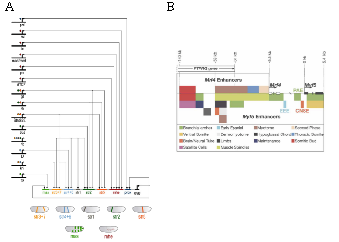
\includegraphics[width=1.0\textwidth]{figures/furlong-carvajal-enhancers-patterns.pdf}
\captionbf{Diff�rents CRMs conduisent � diff�rents patterns d'expression}{
    
    (A) Figure tir�e de \cite{Wilczynski2010p575}, montrant le r�seau de
    cis-r�gulation du g�ne \textit{even-skipped} chez la \textit{Drosophile}.
    Des enhancers individuels (bo�tes color�es) conduisent � des motifs
    d'expression distincts (indiqu�s dans les embryons par la m�me couleur).
    Les cercles color�s au sein des r�gulateurs indiquent les couleurs des CRMs
    r�gul�s.

    (B) Figure tir�e de \cite{Carvajal2008p395}, repr�sentant les diff�rents
    �l�ments r�gulateur du locus \textit{Mrf4}/\textit{Myf5}. Chaque bo�te
    color�e repr�sente une r�gulation de la transcription � un stade de
    d�veloppement particulier ou dans une r�gion anatomique sp�cifique du
    muscle embryonnaire ou adulte.

} 
\label{fig:enhancers-pattern}
\efig
%\end{figure}


%\bfig
%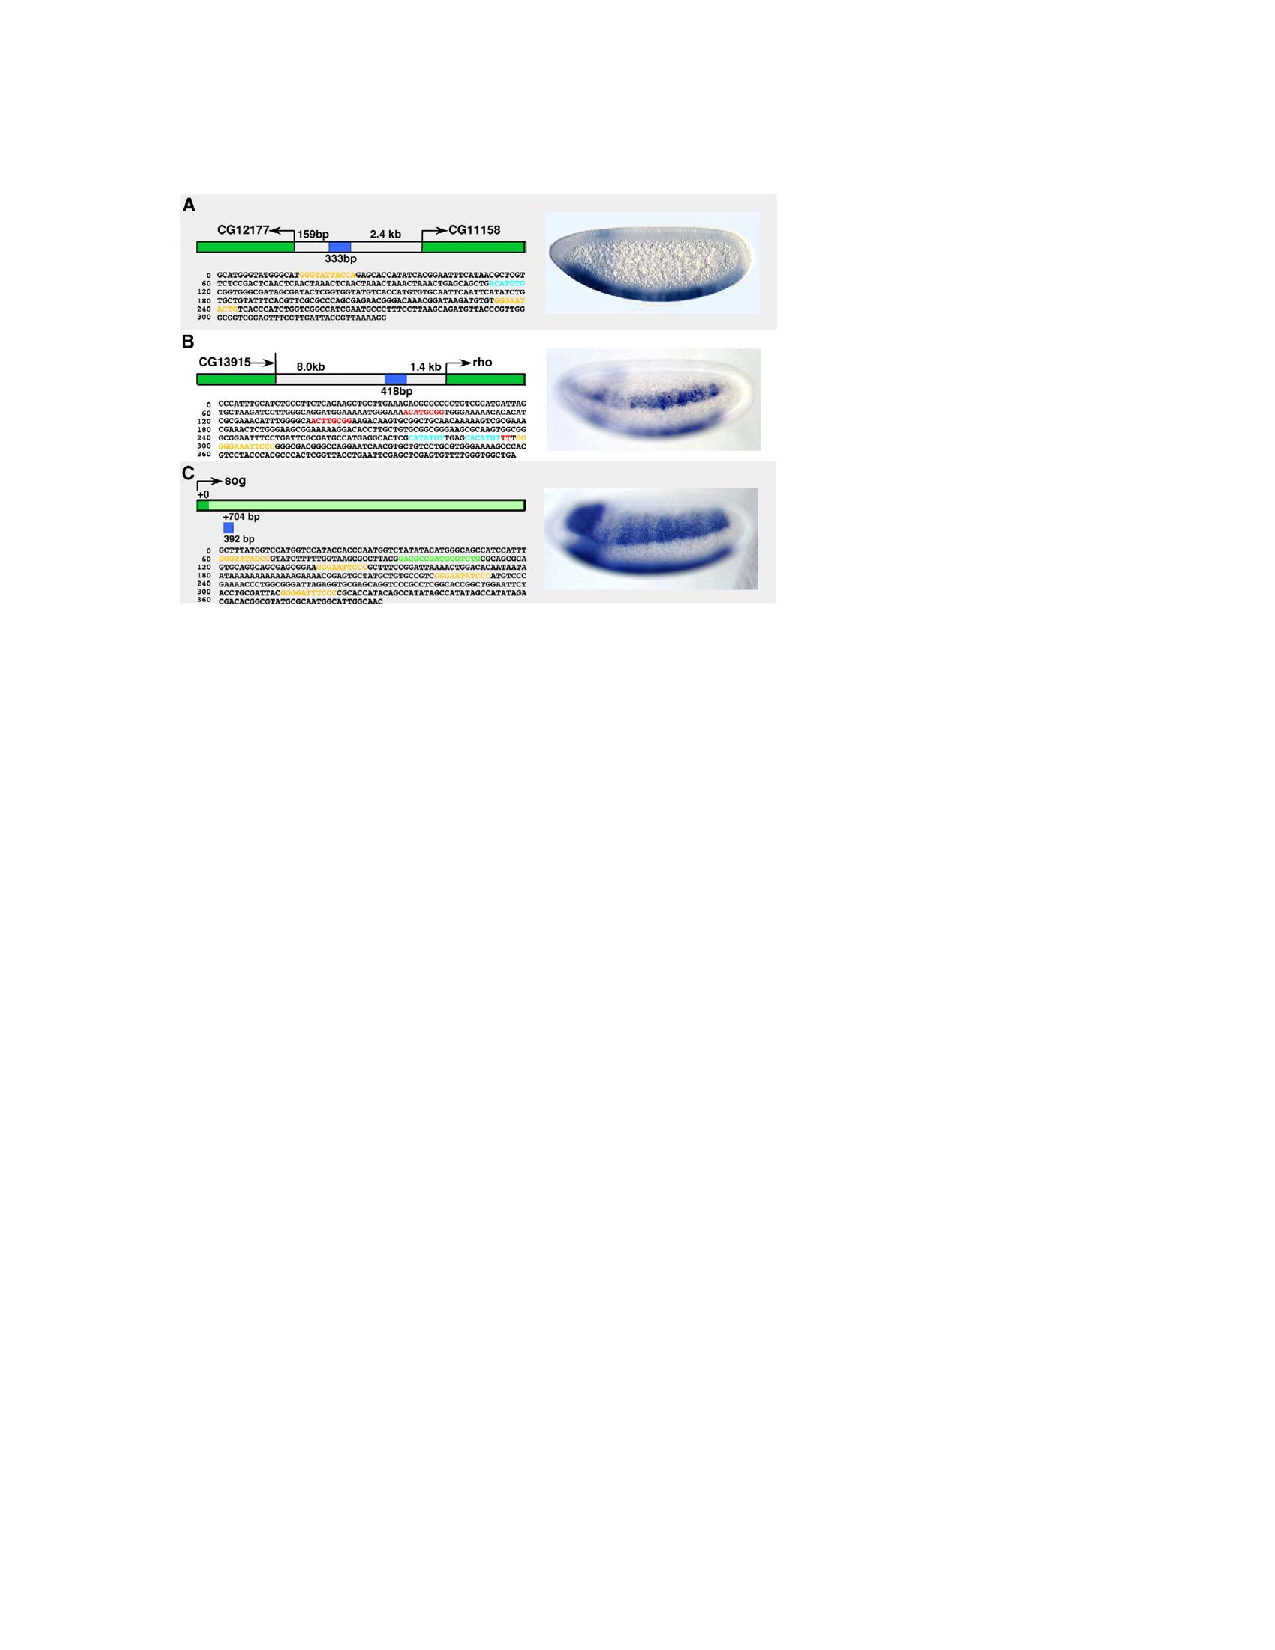
\includegraphics[width=\textwidth]{figures/stathopoulos-CRMs-sites-twist-dorsal-snail.pdf}
%\captionbf{}{
    %Figure tir�e de \cite{Stathopoulos2005p4051}.
%} 
%\efig

\newpage
\subsection{Grammaire des enhancers : enhanceosome vs billboard}


Nous l'avons vu, les CRMs contiennent en g�n�ral de multiples sites de liaisons
(TFBS) pour un ou plusieurs TFs. On parle de \textit{clustering}
(regroupement). Lorsque les TFBS correspondent � plusieurs TFs diff�rents, on
parle de CRM h�t�rotypique, et dans le cas o� ils correspondent � un m�me TF,
on parle de CRM homotypique. Cette distinction est surtout utile pour d�crire
les diff�rentes m�thodes de pr�diction de CRM, car la plupart des CRMs
identifi�s chez les M�tazoaires sont h�t�rotypiques~\cite{Aerts2012p3868}.
L'organisation de ces sites de liaison rel�ve de deux types d'architecture
principaux (fig.~\ref{fig:kulkarni-billboard}).

\begin{figure}
    \centering
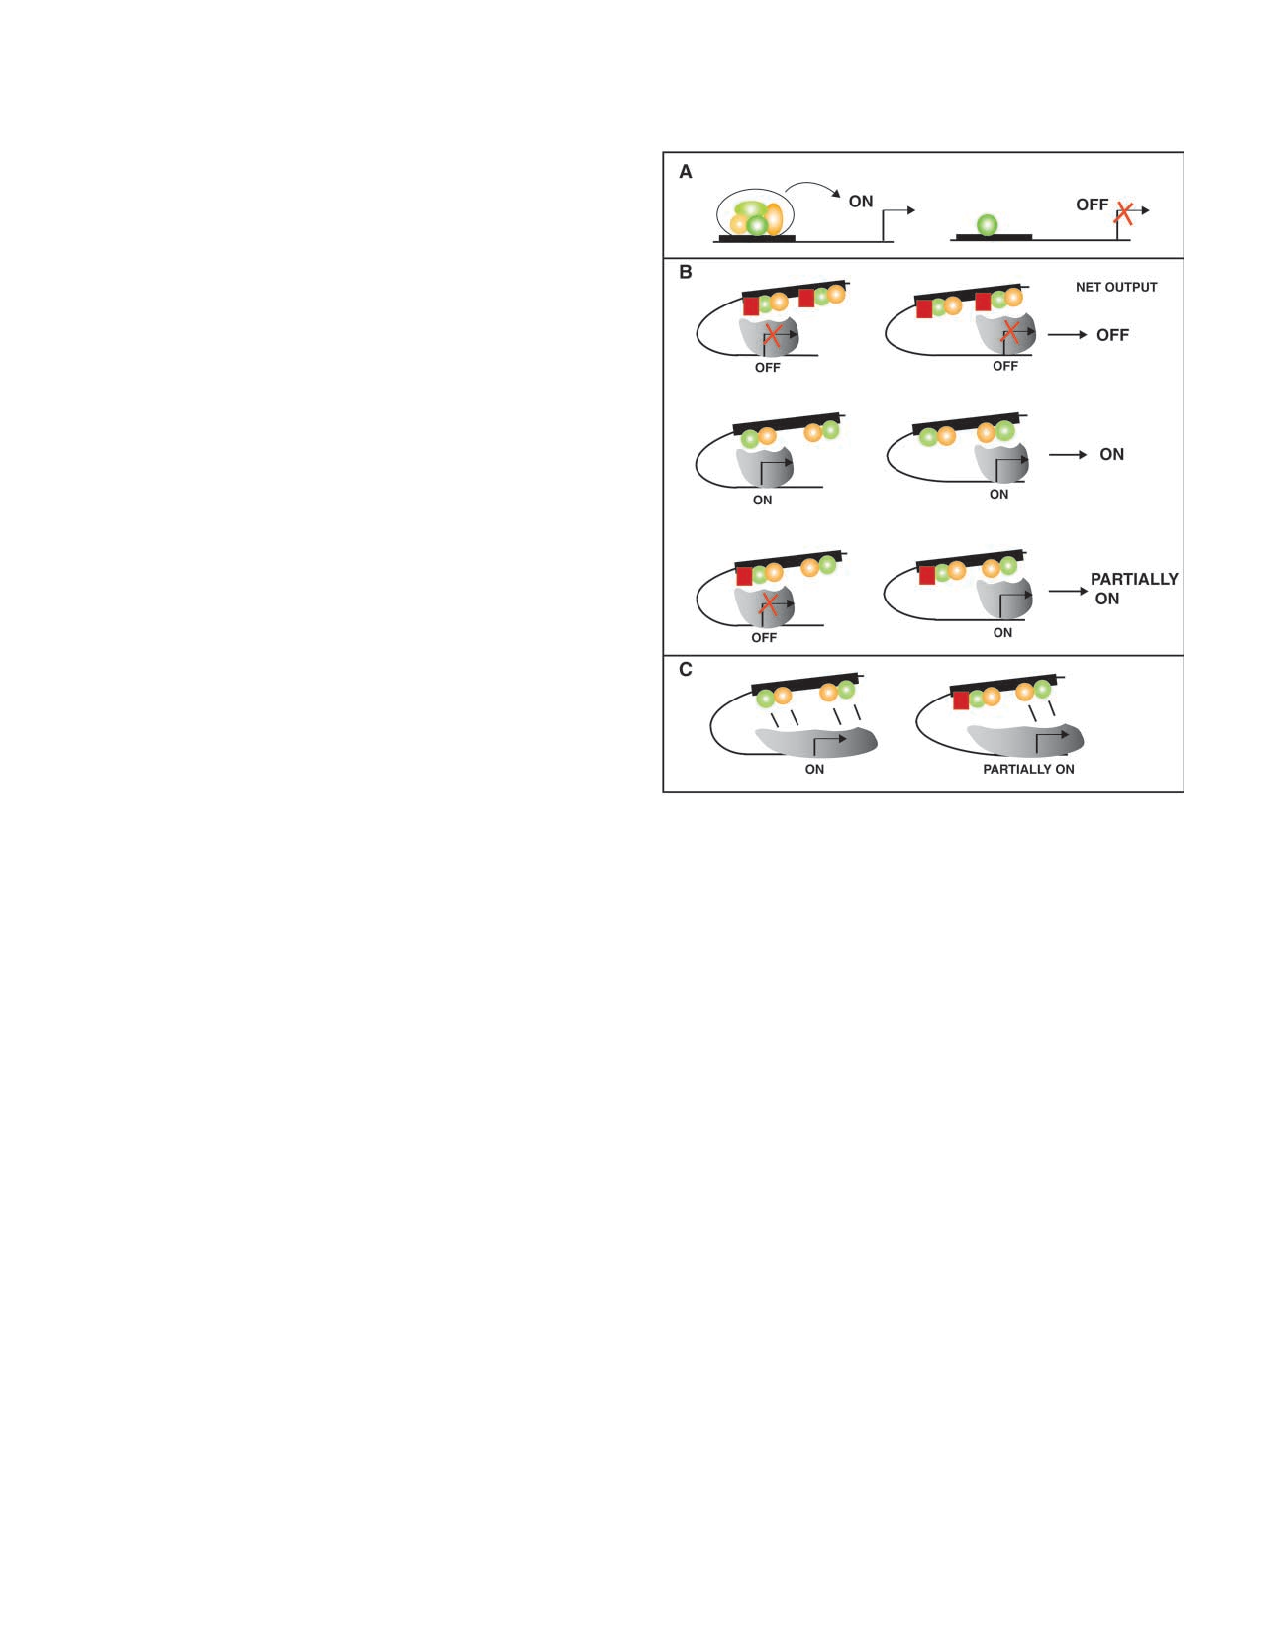
\includegraphics[width=.8\textwidth]{figures/kulkarni-billboard.pdf}
\captionbf{Deux mod�les d'enhancers: enhanceosome et billboard}{

    Figure tir�e de~\cite{Kulkarni2003nx}. (A) Dans le mod�le enhanceosome,
    l'enhancer traite l'information des multiples TFs qui le fixent. Un
    complexe tr�s structur� ou enhanceosome cr�e une interface qui recrute la
    machinerie de transcription basale. L'enhancer peut �tre vu comme un
    ordinateur mol�culaire qui produit � partir d'entr�es multiples un seul
    signal vers la machinerie de transcription. Le g�ne cible n'est activ�
    qu'en cas de formation du complexe entier, ce qui fournit un interrupteur
    binaire on/off seulement activ� en cas de stimulus ad�quat. La
    d�stabilisation du complexe en changeant par exemple la concentration d'une
    des prot�ines permettrait alors d'obtenir une r�ponse graduelle.  (B,C)
    Mod�le d'enhancer ``billboard''. Dans ce cas, l'enhancer ne consiste pas en
    une seule unit� de r�gulation, mais des sous-unit�s peuvent contenir
    diff�rentes informations (r�pression ou activation par exemple) que la
    machinerie basale �chantillonne soit it�rativement (B), soit simultan�ment
    (C).

} 
\label{fig:kulkarni-billboard}
\end{figure}

\subsubsection{Le mod�le ``billboard''}
\label{ssub:le_mod_le_billboard_}

La majorit� des CRMs adh�rent � ce type d'organisation. L'architecture y est
libre : les sites de liaisons n'ont pas de contrainte de nombre, d'ordre, de
sens, ou d'espacement~\cite{Kulkarni2003nx}. De tels CRMs sont propices � une
d�tection informatique bas�e sur la densit� de sites de liaisons pour
diff�rents TFs.

% subsubsection le_mod_le_billboard_ (end)

\subsubsection{Le mod�le ``enhanceosome''}
\label{ssub:le_mod_le_enhanceosome_}

Dans ce mod�le, l'architecture des sites de liaison est de prime importance. Le
paradigme en est l'enhancer du g�ne humain interferon-$\beta$, sur lequel $8$
TFs se fient pour former une surface de reconnaissance
continue~\cite{Panne2008kl}. Les TFBS de cet enhancer se recouvrent les uns les
autres, cr�ant au final un complexe de TFs fix�s � l'ADN agissant comme une
seule unit� de r�gulation (fig.~\ref{fig:panne-enhanceosome}).

\bfig

\includegraphics[width=0.8\textwidth]{figures/panne-enhanceosome.pdf}
\captionbf{L'enhanceosome de l'interferon-$\beta$}{

    Figure tir�e de~\cite{Panne2008kl} repr�sentant le complexe de TFs
    assembl�s sur l'enhanceosome IFN-$\beta$, formant une surface de
    reconnaissance agissant comme une seule unit� de r�gulation.

}
\label{fig:panne-enhanceosome}
\efig


% subsubsection le_mod_le_enhanceosome_ (end)



\newpage
\subsection{�volution des enhancers}

\bfig
\includegraphics[width=\textwidth]{figures/liberman-crm-conservation-flexibility.pdf}
\captionbf{}{
    figure tir�e de \cite{liberman2009p3886}.
} 
\efig

\bfig
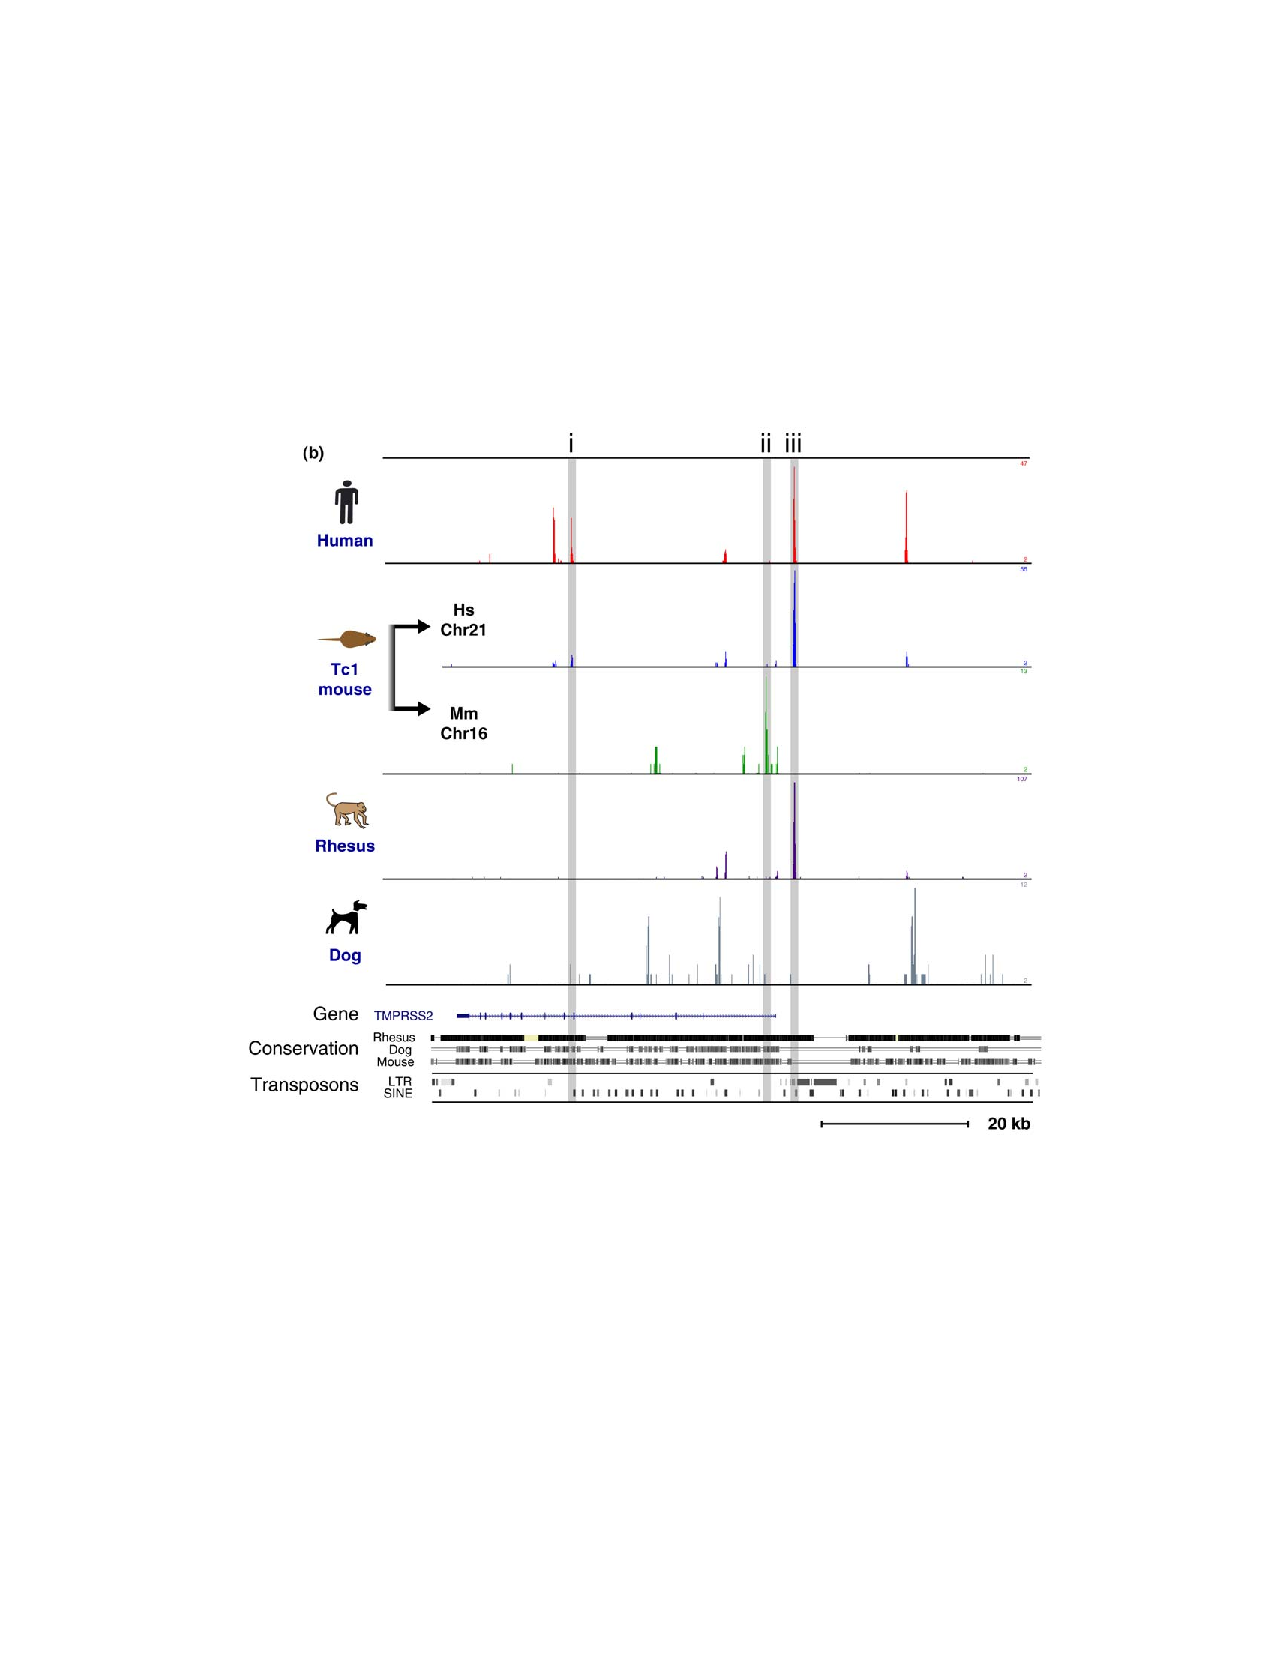
\includegraphics[width=\textwidth]{figures/wilson-CRMs-evolution.pdf}
\captionbf{}{
    figure tir�e de \cite{Wittkopp2011p3240}.
} 
\efig

\cite{Feschotte2008dq}

\newpage
\subsection{Les \og shadow enhancers \fg}

L'�volution des �l�ments de cis-r�gulation est un m�canisme majeur permettant
la diversit� animale. N�anmoins, de tels changements pourraient compromettre
certaines activit�s g�n�tiques essentielles. R�cemment, des exp�riences de
\chipchip ont sugg�r� que plusieurs g�nes de d�veloppement actifs lors du
d�veloppement pr�coce de l'embryon de Drosophile poss�dent des CRMs
secondaires, qui conduisent � des motifs d'expression g�n�tique comparables
� ceux produits par des CRMs \og primaires \fg plus
proximaux~\cite{Zeitlinger2007ly}. L'expression de \og shadow enhancer \fg
a �t� propos�e par Michael Levine en 2008 pour d�crire ces CRMs redondants et
souvent distaux de plusieurs dizaines de kb du g�ne r�gul�~\cite{Hong2008zr}.
Il est probable que de tels CRMs soient apparus au cours de l'�volution par
duplication du CRM primaire, � l'instar du ph�nom�ne de duplication des
s�quences codant pour des prot�ines.  L'avantage �vident que peut conf�rer la
redondance d'un �l�ment de r�gulation est d'offrir de la robustesse face aux
mutations. Par ailleurs, une telle redondance permet de faciliter la divergence
et donc la sp�cialisation des diff�rents CRMs. Ainsi les \se semblent �voluer
plus rapidement que les CRMs primaires auxquels ils sont
apparent�s~\cite{Hong2008zr} pour fournir de nouveaux sites de fixation et
conduire � de nouvelles activit�s de r�gulation sans bloquer la fonction
critique de certains g�nes de d�veloppement.
\\

Un exemple m�lant robustesse et divergence est le
cas des multiples CRMs r�gulant le g�ne \textit{Svb} chez la Drosophile.
Chaque CRM est li� � la production d'un motif distinct de trichomes
(excroissances de l'�pith�lium comparables � des poils) sur la larve : ainsi,
plusieurs mutations dans ces diff�rents CRMs sont n�cessaires pour observer un
changement morphologique cons�quent~\cite{McGregor2007p400}. Dans ce m�me
syst�me, il a �t� montr� que deux CRMs suppl�mentaires, des \se, sont
dispensables dans des conditions de temp�rature usuelles, mais requis lorsque
les embryons se d�veloppent dans des conditions de temp�rature
extr�mes~\cite{Frankel2010p463}.
\\

Par ailleurs, il a �t� montr� que les g�nes gap de la Drosophile poss�dent tous
des \se, dont le r�le semble �tre d'assurer une plus grande pr�cision spatiale
du motif d'expression du g�ne r�gul�~\cite{Perry2011ve}. La perte de l'un des
CRMs, proximal comme \se, conduit � une expression trop restreinte ou trop
r�pandue spatialement selon le cas.
\\


\newpage
\subsection{Les super enhancers}
\label{sub:les_super_enhancers}


\bfig
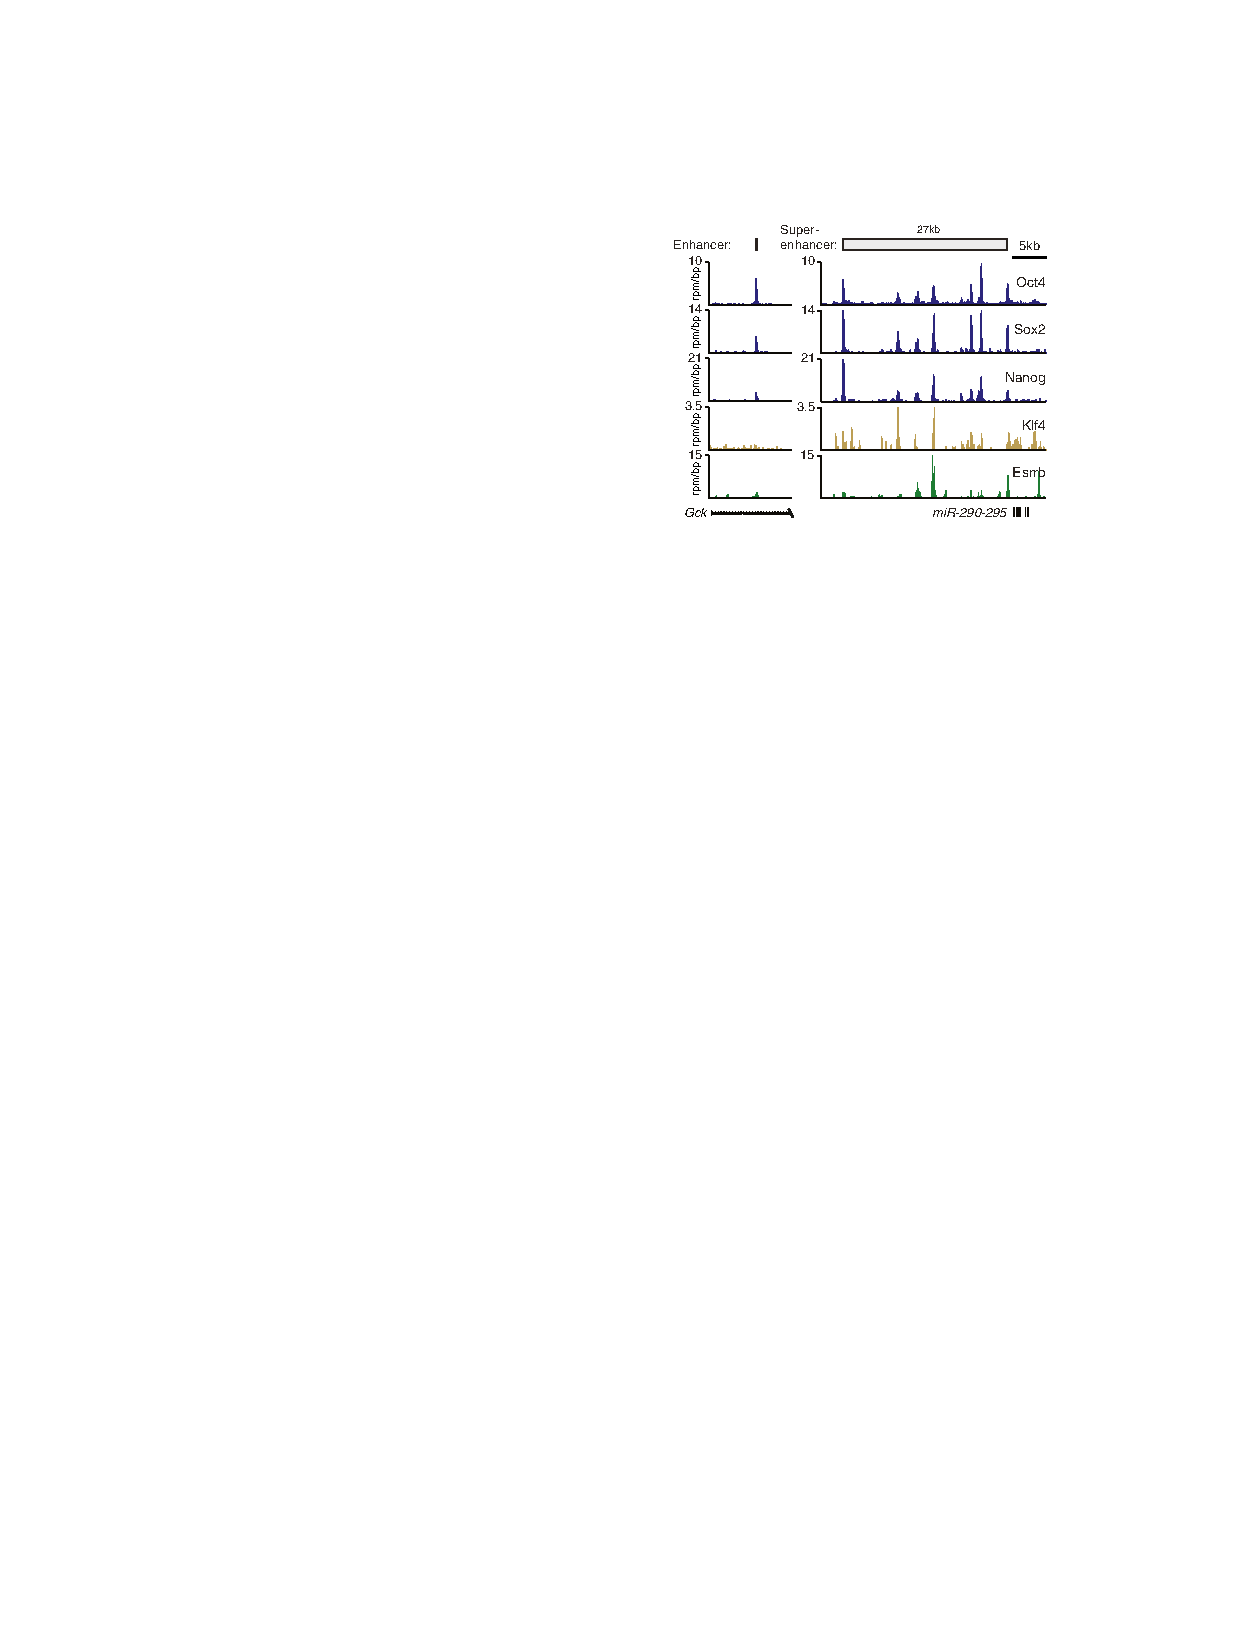
\includegraphics[width=0.8\textwidth]{figures/whyte-super-enhancer-cluster.pdf}
\captionbf{De l'enhancer au super-enhancer}{

    Figure tir�e de~\cite{Whyte2013tg}, montrant les profils de \chipseq des
    TFs ma�tres Oct4, Sox2, Nanog, Klf4 et Esrrb aux loci de \textit{Gck} et
    \textit{miR-290-295} dans les cellules souches embryonnaires. Le
    super-enhancer se distingue du simple enhancer par sa taille ($27$kb), sa
    grande concentration en TFs ma�tres, notamment Klf4 et Esrrb, et la
    fixation de la prot�ine Med1 du complexe Mediator.

}
\label{fig:whyte-super-enhancer}
\efig

R�cemment, il a �t� montr� que certains groupements d'enhancers peuvent agir
comme une m�me unit� de r�gulation : on parle de \textit{super-enhancers}
\cite{Whyte2013tg}. Ces r�gions de taille typique $\sim10$kb
(fig.~\ref{fig:whyte-super-enhancer}), sont fix�es par des TFs ma�tres et sont
associ�es � des g�nes encodant des r�gulateurs cl�s de l'identit� cellulaire.
Identifi�s dans les cellules souches embryonnaires (ESCs), ces ensembles
d'enhancers sont fix�s par le complexe co-activateur Mediator, qui interagit
avec la coh�sine pour former un anneau permettant de connecter la r�gion de
r�gulation au promoteur~\cite{Kagey2010p606}. Par ailleurs, les g�nes associ�s
aux super-enhancers poss�dent un niveau particuli�rement �lev� d'expression et
leur absence est associ�e � une perte de l'�tat souche des cellules.

Ainsi, ce second niveau d'organisation de la r�gulation pourrait simplifier la
mod�lisation de la r�gulation du type cellulaire, en passant de millier de
traces de fixation pour diff�rents TFs � quelques centaines de super-enhancers
contr�lant les g�nes cl�s de l'identit� cellulaire.

% subsection les_super_enhancers (end)

\subsection{Validation exp�rimentale}
\label{sub:validation_experimentale}

Lorsqu'un CRM est pr�dit, il existe plusieurs m�thodes pour s'assurer de sa fonctionnalit�. 

Tout d'abord, une m�thode indirecte donnant du cr�dit � la pr�diction d'un CRM
est d'examiner le motif d'expression du g�ne dont le TSS est le plus proche. Si
cette expression reproduit les caract�ristiques utilis�es pour pr�dire le CRM
(par exemple, s'exprimer dans le muscle pour une pr�diction de CRMs utilisant
l'abondance de sites de liaison de TFs musculaires), alors cela soutient l'id�e
(mais ne la d�montre pas) que la pr�sence du CRM en est la cause.

Une m�thode plus directe permettant de d�montrer qu'un fragment d'ADN r�gule
l'expression g�n�tique consiste en une exp�rience de gain de fonction dans
laquelle un plasmide contenant le CRM pr�dit � proximit� d'un g�ne rapporteur
est introduit par transfection \invitro en cellule, permettant un suivi
quantitatif de l'activit�, ou par transgen�se \invivo dans un organisme, auquel
cas le suivi est plus qualitatif mais permet d'�tablir la sp�cificit�
spatio-temporelle (tissu et stade de d�veloppement) de l'�l�ment de r�gulation
(fig.~\ref{fig:hardison-CRM-test}). Ce type d'exp�rience montre que le CRM
pr�dit est \textit{suffisant} pour reproduire le motif g�n�tique observ�. De
mani�re optimale, il faudrait aussi montrer par d�l�tion cibl�e de l'�l�ment de
r�gulation au sein du g�nome que ce dernier est \textit{n�cessaire}
� l'expression du g�ne endog�ne.

\bfig
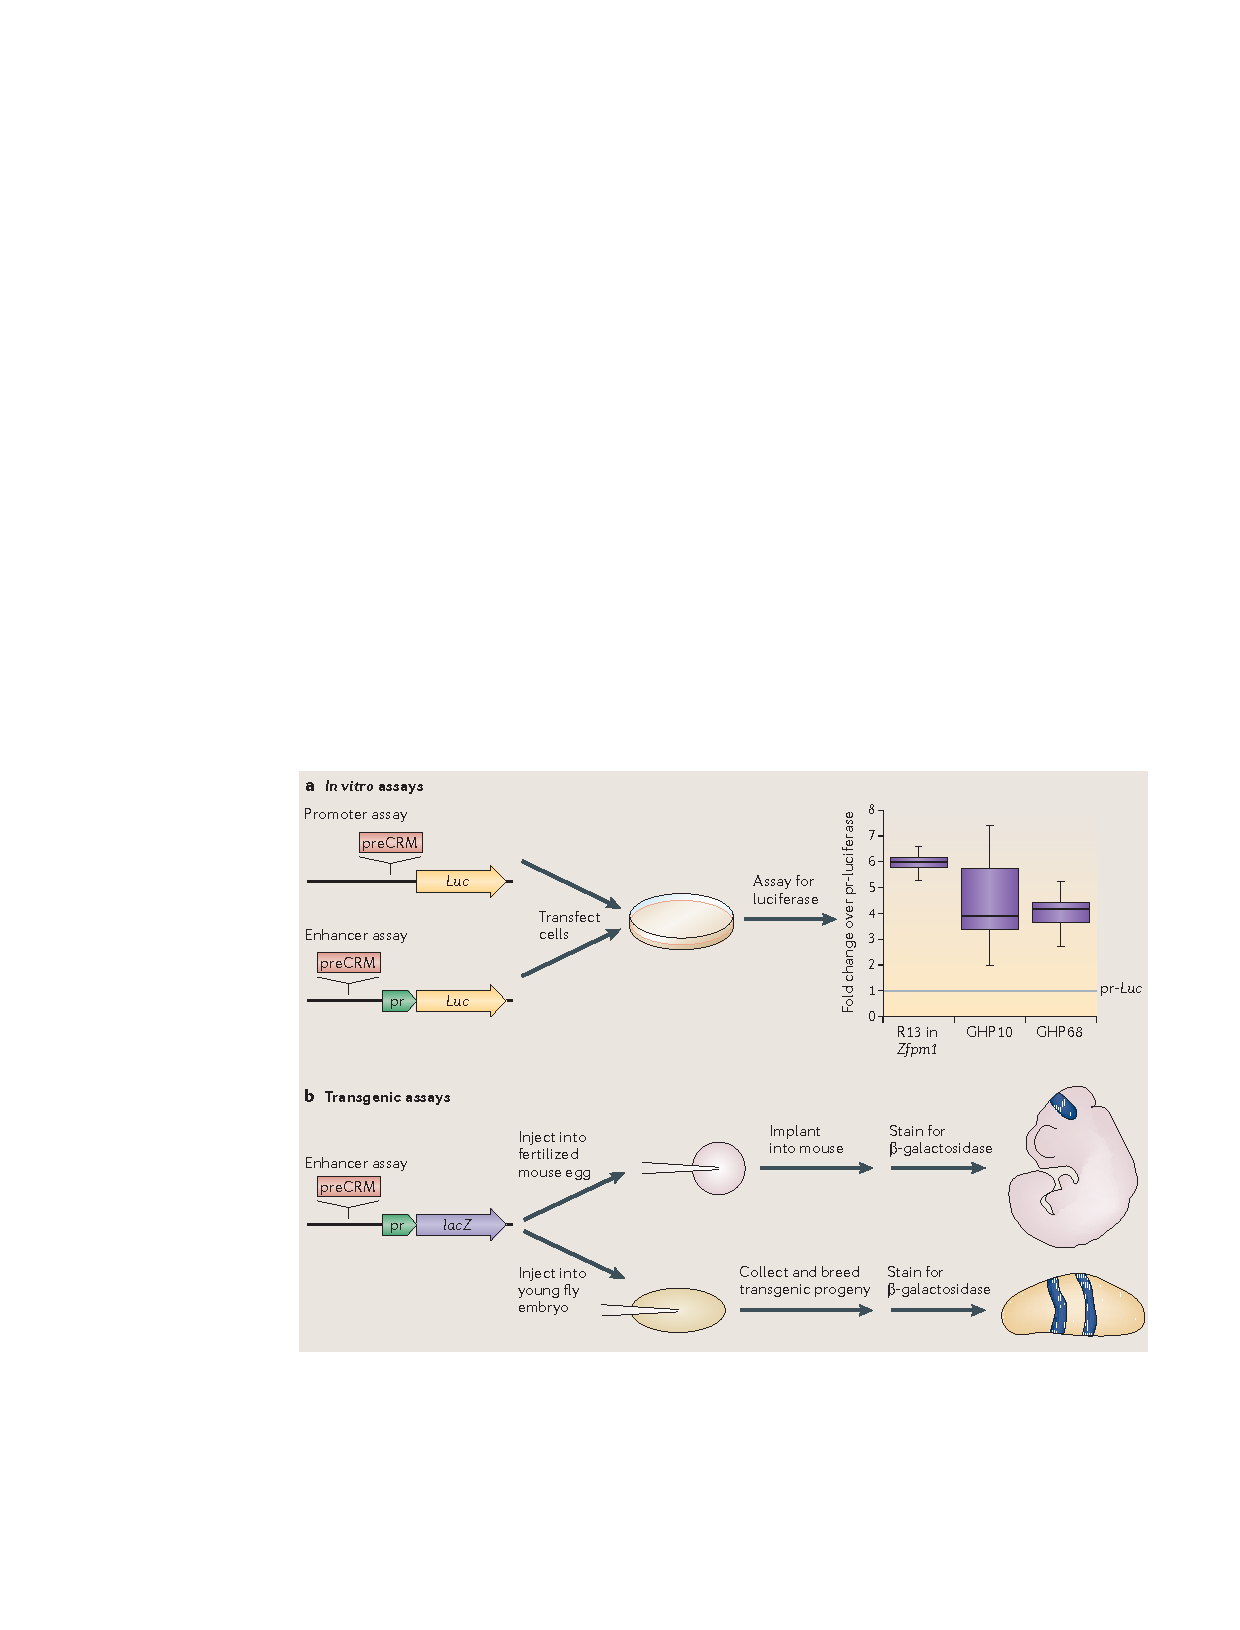
\includegraphics[width=\textwidth]{figures/hardison-CRM-test.pdf}
\captionbf{M�thodes de validation des CRMs par transfection et transgen�se}{
    
    Figure tir�e de \cite{Hartwell1999p560} pr�sentant les m�thodes \invitro et
    \invivo de validation des CRMs. La r�gion dont on souhaite tester
    l'activit� est ins�r�e dans un plasmide codant pour un g�ne rapporteur qui
    est transf�r� dans une culture cellulaire (transfection, panel a) ou dans
    un organisme entier (transgen�se, panel b). Dans le cas du test d'un
    promoteur, le CRM est plac� directement en amont du g�ne rapporteur (on
    utilise g�n�ralement la lucif�rase \textit{Luc}), alors que dans le cas
    d'un enhancer, le CRM est plac� en amont d'un promoteur minimal de faible
    activit�. L'activit� de la lucif�rase donne une information quantitative
    sur l'activit� de la r�gion test�e (bo�tes � moustache, panel a). Dans le
    cas d'une transgen�se, le g�ne rapporteur g�n�ralement utilis� est
    \textit{lacZ} qui encode la $\beta$-galactosidase. La r�v�lation par
    coloration permet de visualiser en bleu les tissus au sein lesquels
    l'enhancer est actif.

} 
\label{fig:hardison-CRM-test}
\efig


%\bfig
%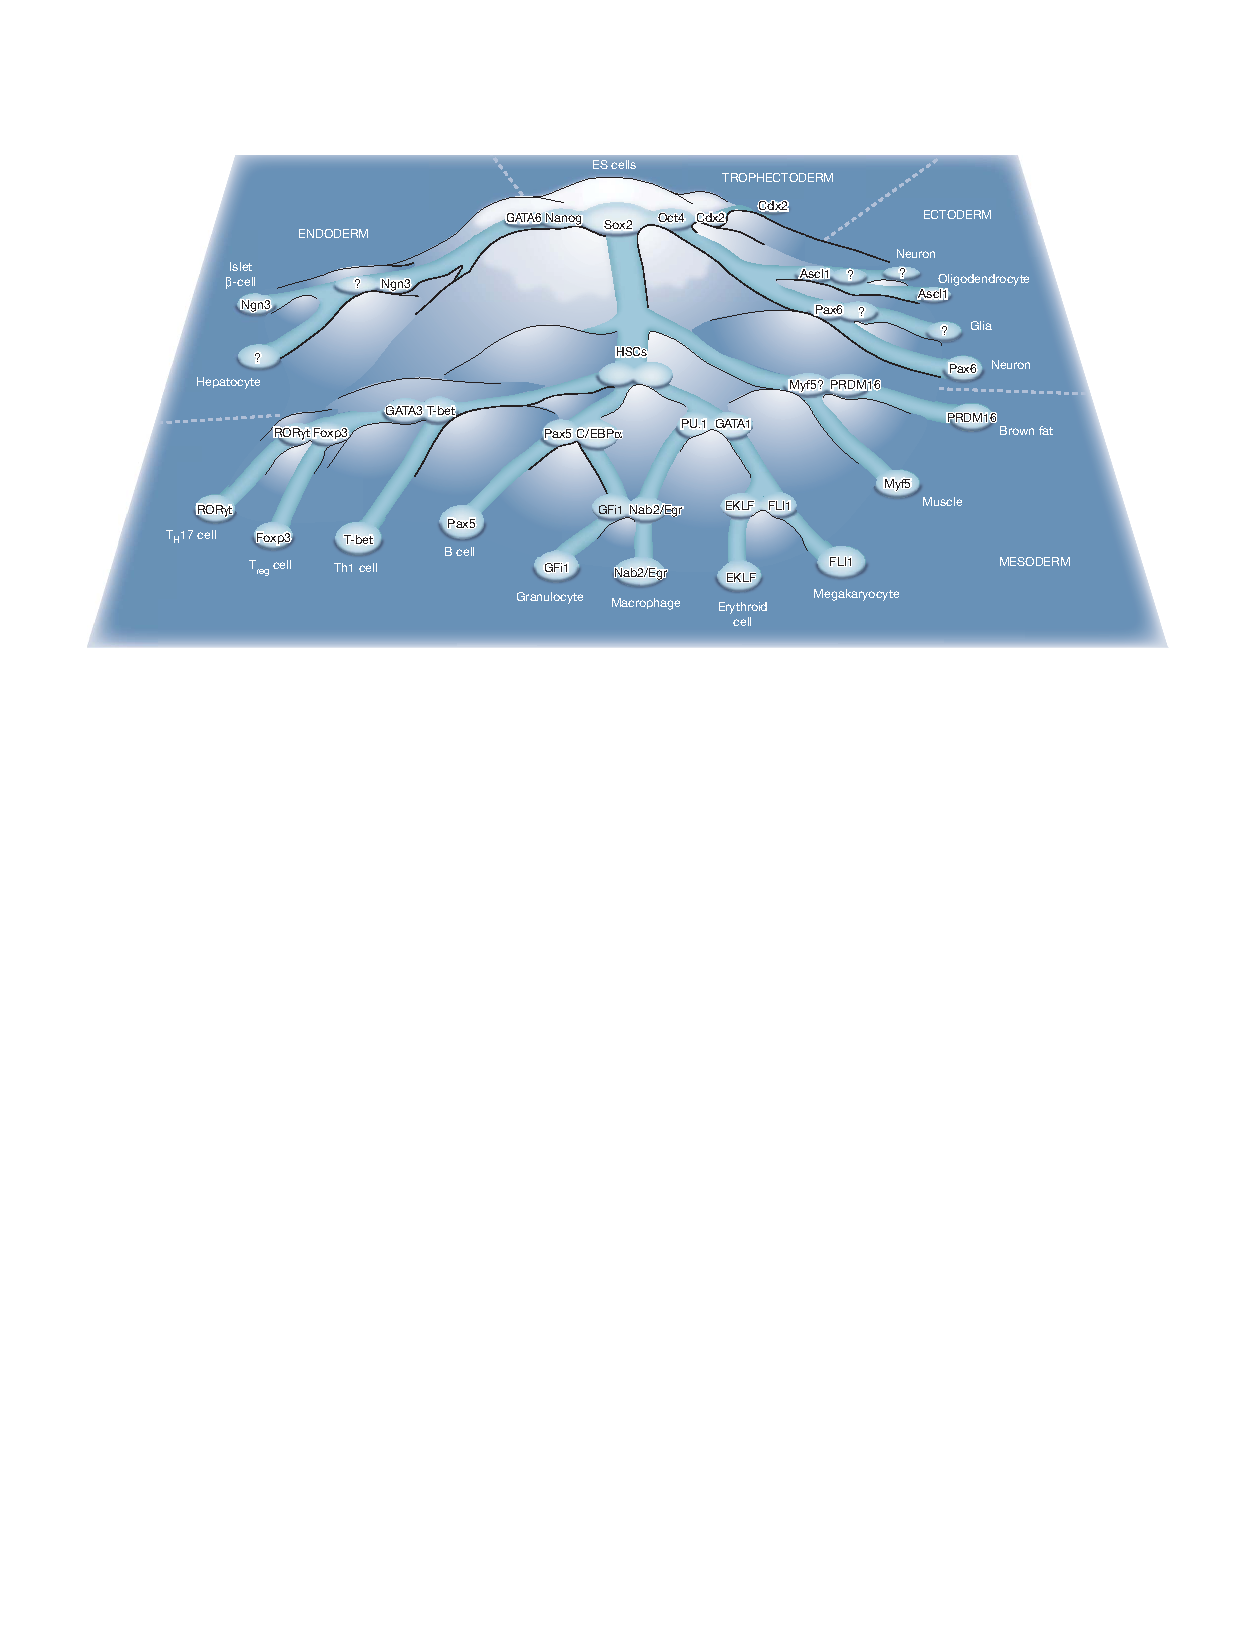
\includegraphics[width=\textwidth]{figures/graf-differentiation-landscape.pdf}
%\captionbf{Les antagonismes entre \tfs sculptent le paysage des destins
%cellulaires}{
%   Figure tir�e de \cite{Graf2009p2592}. Vision g�om�trique de la
%   diff�renciation cellulaire inspir�e de Waddington (voir
%   fig.\ref{fig:furusawa-epigenetic-landscape}).
%} 
%\efig
%

\newpage
\subsection{Pr�diction des CRMs}

\bfig
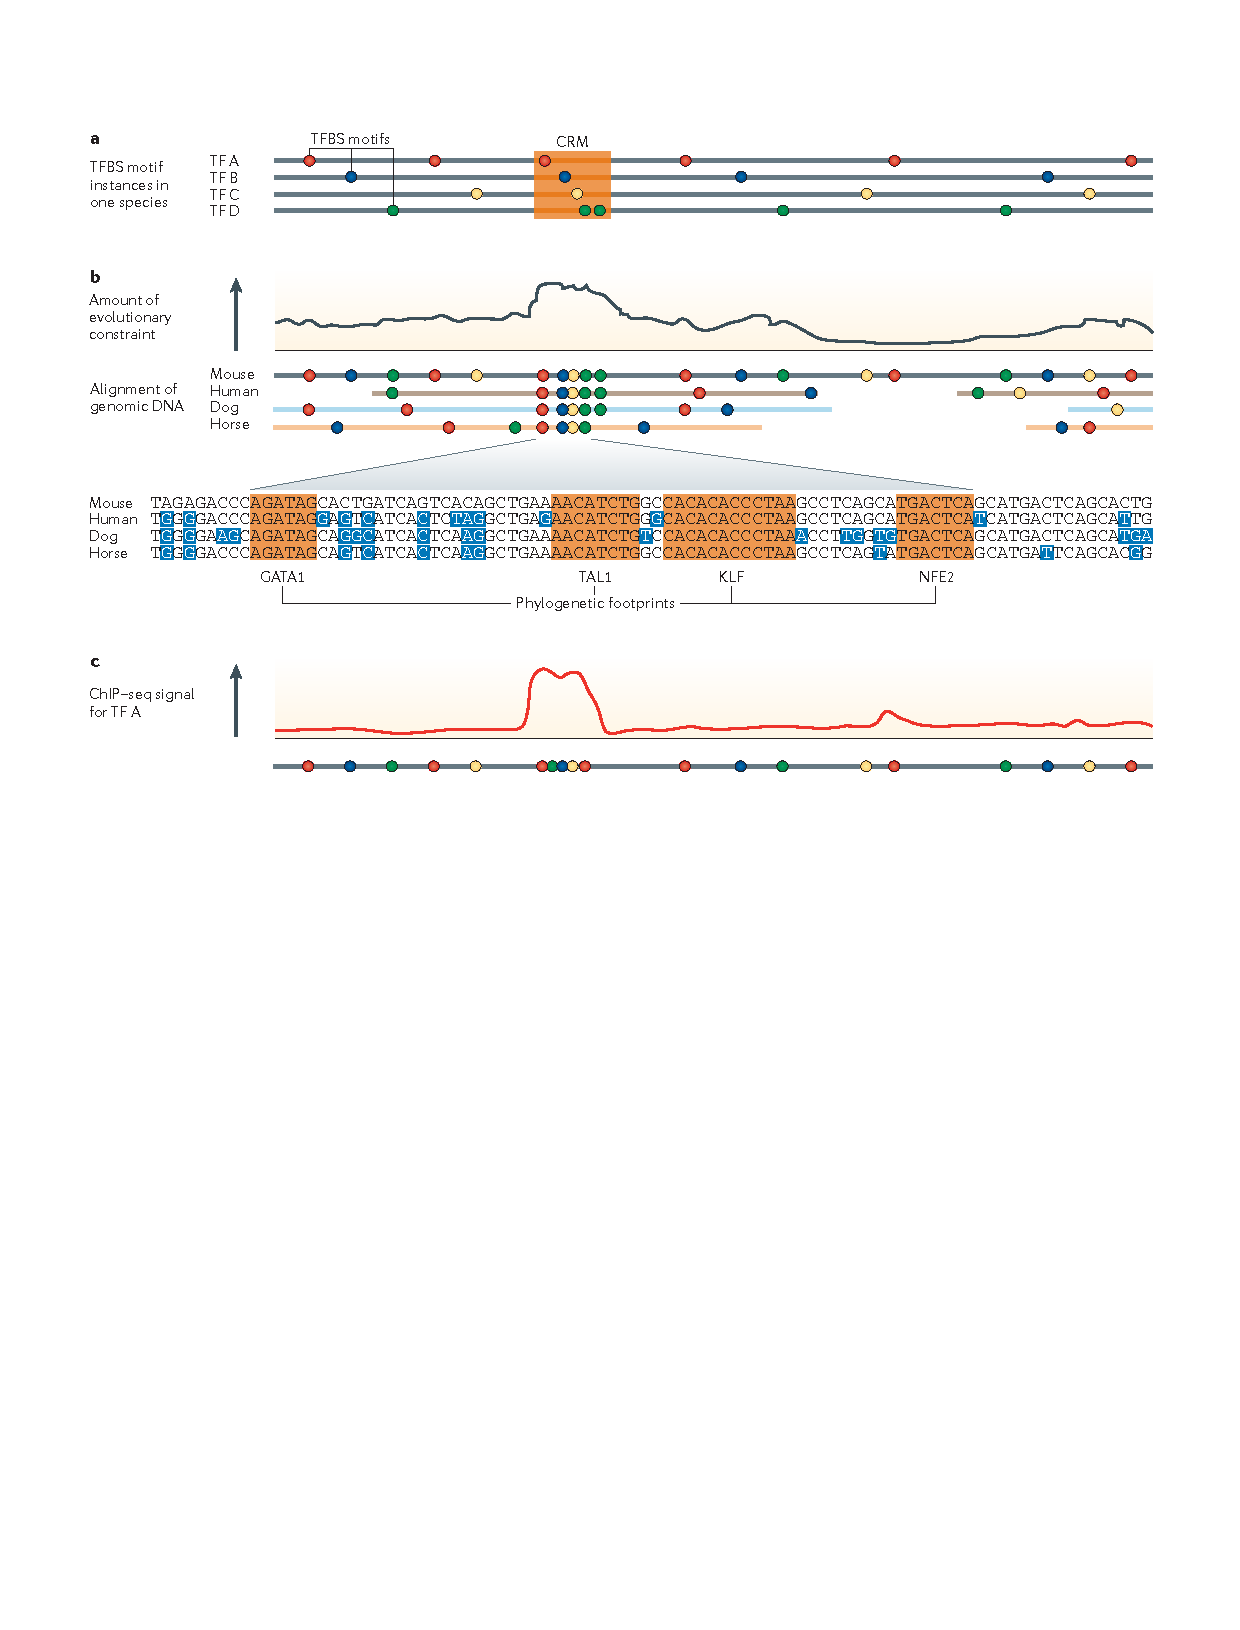
\includegraphics[width=\textwidth]{figures/hardison-CRM-prediction.pdf}
\captionbf{Approches pour la pr�diction des CRMs}{
    Figure tir�e de \cite{Hartwell1999p560}.
} 
\efig

\section{Banques de donn�es}

\subsection{S�quences g�nomiques et alignements}

\bfig
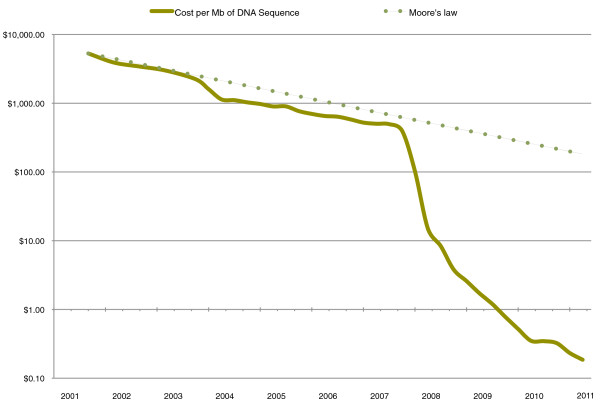
\includegraphics[width=0.8\textwidth]{figures/sboner-cost-sequencing.jpg}
\captionbf{�volution du co�t de s�quen�age}{
Figure tir�e de~\cite{Sboner2011fk}.
}
\label{fig:sboner-cost-sequencing.jpg}
\efig

statistiques du genome (lognormal)
\subsection{Annotations (TSSs, repeats\ldots)}
\subsection{Jaspar et Transfac}
\subsection{Visualisation sur UCSC}
\subsection{Le projet ENCODE}



%\bfig
%
\includegraphics[width=0.8\textwidth]{figures/siggia-fate.pdf}
%\captionbf{Vision g�om�trique des transitions entre types cellulaire}{
%   Figure tir�e de \cite{Corson2012p3973} sch�matisant le processus de
%   diff�renciation des cellules de la vulve de \celegans.
%   \textbf{A.} La cellule est dans un �tat pr�curseur repr�sent� par une
%   bille au fond d'une vall�e.
%   \textbf{B.} La cellule est dans �tat dit \textit{comp�tent} o� elle peut basculer
%   vers diff�rents destins cellulaires.
%   \textbf{C.} Un signal externe repr�sent� par une fl�che rouge modifie le
%   paysage de mani�re � favoriser l'un des �tats finaux possibles.
%} 
%\efig

%\bfig
%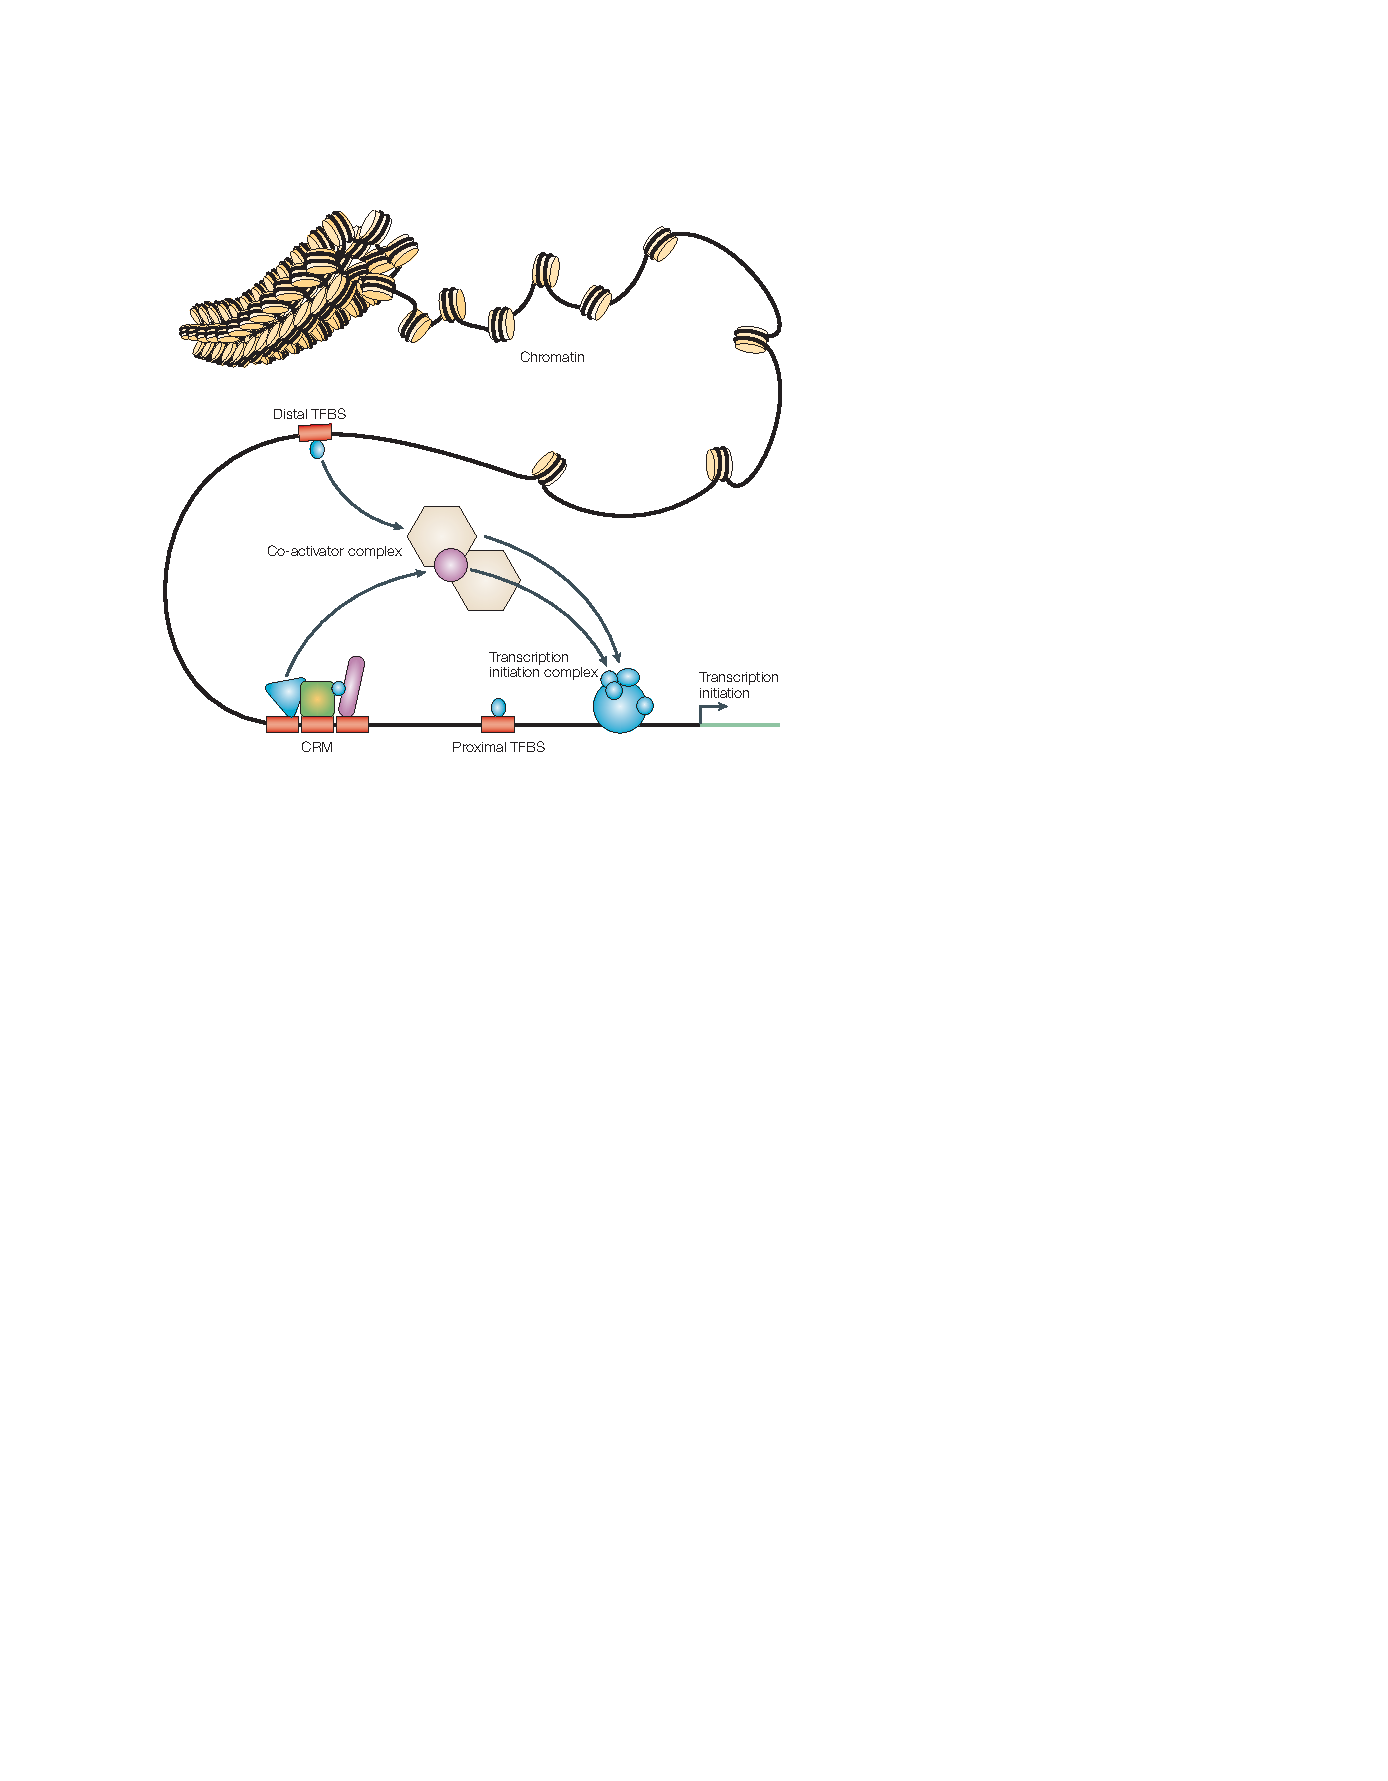
\includegraphics[width=.8\textwidth]{figures/wasserman-transcriptional-regulation.pdf}
%\captionbf{Les diff�rentes composantes de la r�gulation transcriptionnelle}{
    %Figure tir�e de \cite{Wasserman2004p624}. Les \TFs se fixent � des sites
    %sp�cifiques de longueur $\sim10$bp qui peuvent �tre proximaux (promoteur,
    %premiers introns) ou distaux (plus de $100$kb) d'un \TSS. Diff�rents \TFs
    %peuvent s'assembler sur des r�gions d'ADN de taille typique $\sim 1000$bp
    %appel�es \CRMs afin de conduire � une r�gulation sp�cifique, par simple
    %effet de communaut� par exemple lorsque la fixation de tous les \tfs est
    %requise pour que la r�gulation op�re. Les interactions entres les \tfs et
    %diff�rents cofacteurs stabilisent la machinerie d'initiation de
    %transcription pour permettre l'expression g�n�tique. La r�gulation distale
    %est quant � elle fortement d�pendante de la structure tridimensionnelle de
%la chromatine.  } \efig


\newpage 

%%%%%%%%%%%%%%%%%%%%%%%%%%%%%%%%%%%%%%%%%%%%%%%%%%%%%%%%%%%%%%%%%%%%%%%%%%%%%%%%%%%%%%%%%%
\chapter{\ChMaxent} 
\label{ch:maxent}
%\adjustmtc
\minitoc
\newpage
\section*{Introduction du chapitre \thechapter}

Dans cette partie, nous nous int�ressons � la description de l'interaction
entre les \fts et leurs sites de reconnaissance sur l'ADN, interaction qui est
au c{\oe}ur des r�seaux g�n�tiques.  Pendant longtemps, la qualit� de cette
description a �t� limit�e par la quantit� de donn�es disponibles. Ainsi, les
exp�riences de type SELEX (voir \ref{sub:approches_invitro}), o� des
exp�riences de \chip au cas par cas permettaient de r�cup�rer de l'ordre de
quelques dizaines de sites de fixation pour un TF d'int�r�t. Or, le mod�le PWM,
qui est le mod�le le plus simple (en terme de nombre de param�tres) que l'on
puisse b�tir pour d�crire l'interaction poss�de d�j� plusieurs dizaines de
param�tres -- les fr�quences des nucl�otides � chaque position --. 

Ces donn�es ne permettaient donc pas d'explorer plus en avant des mod�les plus
complexes de fixation, o� par exemple on inclurait des termes d'interaction
entre nucl�otides au sein des sites de fixation. Cependant, les avanc�es
r�centes en s�quen�age � haut d�bit ont permis l'obtention de donn�es tr�s
grande �chelle, que ce soit \invivo par \chipseq ou \invitro par HT-SELEX (voir
\ref{sec:mesures_exp}). Le nombre de sites de fixation obtenus est de l'ordre
de quelques milliers, ce qui permet de contraindre des mod�les de fixation plus
complexe que le mod�le PWM.

En utilisant des donn�es \chipseq pour un grand nombre de \fts de la Drosophile
et des vert�br�s, nous avons construit diff�rents mod�les de fixation incluant
implicitement ou explicitement des interactions entre nucl�otides afin de juger
de leur importance dans la description de l'interaction TF-ADN \invivo. Nous
pr�sentons pr�alablement un survol des observations et mod�les existant au
sujet des corr�lations dans les sites de fixations de \fts.

\section{Observations de corr�lations au sein des TFBS}
\label{sec:corr_lations_au_sein_des_sites_de_fixation_de_tfs}

Diff�rents travaux ont mis en exergue l'existence de corr�lations entre
nucl�otides au sein des sites de fixation de TFs. Parce que limit�es par la
quantit� de donn�es alors possible d'obtenir, les premi�res �tudes de ce genre
ont centr� leur attention sur les corr�lations importantes pour quelques cas
particuliers. Ainsi, \citet{Man2001fk} ont observ� que la prot�ine Mnt induit
des corr�lations entre les positions $16$ et $17$ de ses sites de
reconnaissance \invitro. Ils ont mesur� exp�rimentalement la sp�cificit� aux
sites de liaisons contenant tous les variants possibles � ces deux positions.
Ils ont ainsi observ� que la mutation de la base consensus C en position 17
induisait un changement de pr�f�rence en position 16 de la base A vers la base
C. Par ailleurs, \citet{Bulyk2002uq} ont montr� que la prot�ine EGR1 induisait
des corr�lations au sein d'un triplet de nucl�otides central de leur site de
reconnaissance. La prise en compte de ces corr�lations dans l'�nergie de
fixation permettait alors d'am�liorer la description des donn�es par rapport au
mod�le additif PWM.

� une plus grande �chelle, \citet{Badis2009p3911} ont utilis� des puces � ADN
(technique PBM, cf \ref{sub:approches_invitro}) pour �tudier la fixation
\invitro de $104$ TFs de la souris sur toutes les s�quences d'ADN de $10$ bp
possibles. Pour chaque facteur, plusieurs centaines de s�quences de fixation
ont ainsi �t� obtenues. L'�tude a r�v�l� l'existence d'une multiplicit� de
motifs (PWMs) pour la plupart des TFs (seulement $15$ �tant mieux d�crit par un
motif unique). Certains motifs reconnaissent notamment des s�quences
� espacement variable pour lesquelles deux r�gions sp�cifiques du site sont
s�par�es par un nombre variable de nucl�otides. Enfin, les auteurs ont not� la
pr�sence de corr�lations fortes dans $19$ cas, celles-ci n'�tant pas forc�ment
limit�es � des dinucl�otides mais pouvant impliquer des trinucl�otides. Plus
r�cemment, \citet{Jolma2013p3971} ont analys� par HT-SELEX plusieurs centaines
de domaines de fixations � l'ADN de TFs humains et de la souris, r�v�lant aussi
l'importance d'espacements variables et surtout des corr�lations
dinucl�otidiques entre plus proches voisins.


\section{Mod�les existants permettant de d�crire la statistique des TFBS}
\label{sec:mod_les_pour_d_crire_les_corr_lations}

Diff�rents mod�les ont �t� propos�s pour d�crire ces corr�lations
(fig.~\ref{fig:modeles-correlations}). La m�thode la plus directe consiste
� partir du mod�le PWM (fig.~\ref{fig:modeles-correlations}a) et � ajouter des
corr�lations mutuellement exclusives aux positions les plus corr�l�es
(fig.~\ref{fig:modeles-correlations}b). D'autres m�thodes utilisent des
structures probabilistes de d�pendances sous forme de cha�nes de Markov
(fig.~\ref{fig:modeles-correlations}c) ou plus g�n�ralement de r�seau bay�sien
ou (fig.~\ref{fig:modeles-correlations}d-e), rendant alors l'interpr�tation
moins �vidente. Enfin, il est possible de r�aliser des m�langes de mod�les afin
de capturer des ensembles distincts de corr�lations
(fig.~\ref{fig:modeles-correlations}f-g). Nous recensons ici ces diff�rents
mod�les.

\bfig
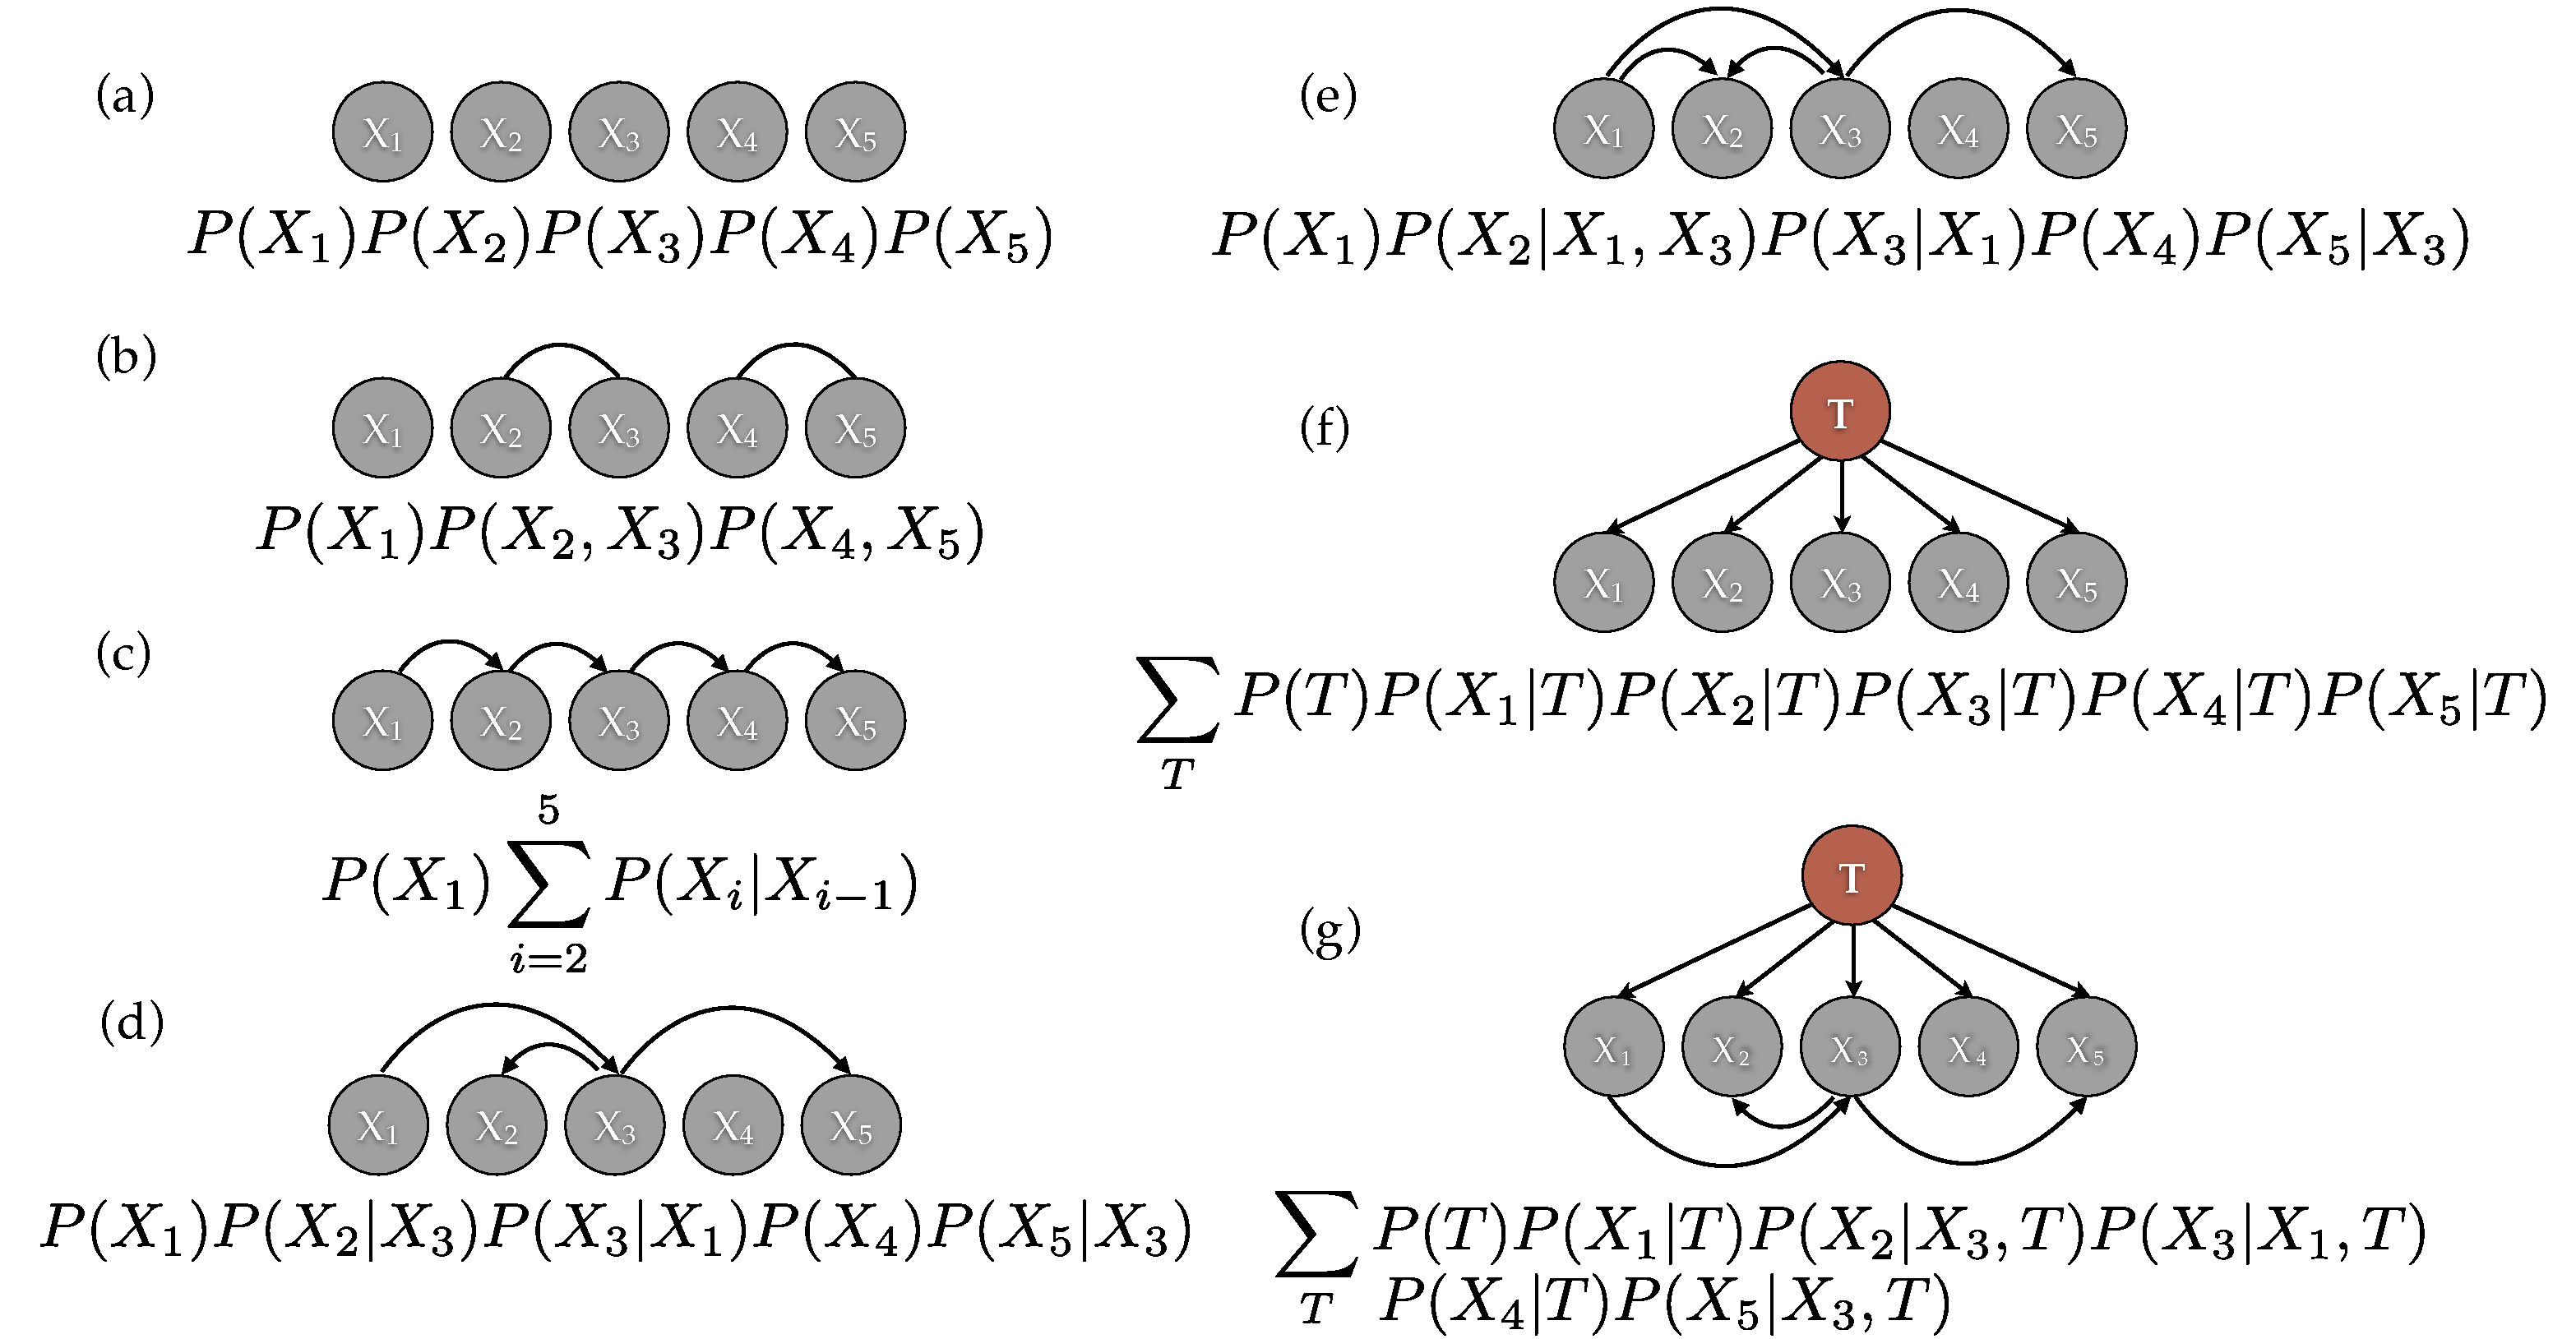
\includegraphics[width=1\textwidth]{figures/modeles-correlations.pdf}
\captionbf{Diff�rents mod�les pour d�crire les corr�lations entre nucl�otides dans les sites de fixation de \fts}{

    Exemples illustrant diff�rents mod�les de fixation sur un site de longueur
    $5$. Pour chaque mod�le, la structure du r�seau de d�pendances sous-jacent
    est repr�sent�e, ainsi que la distribution de probabilit�
    $P(X_1,X_2,X_3,X_4,X_5)$ correspondante, o� $X_i$ correspond au nucl�otide
    (A, C, G ou T) � la position $i$. Les mod�les repr�sent�s sont les suivants
    :
    (a) PWM (pas de corr�lations), 
    (b) GWM (corr�lations mutuellement exclusives), 
    (c) cha�ne de Markov d'ordre $1$ (corr�lations entre plus proches voisins), 
    (d) r�seau bay�sien en arbre (au plus un parent par n{\oe}ud) ou 
    (e) pas en arbre (le n{\oe}ud $2$ a deux parents), 
    (f) m�lange de PWMs et 
    (e) m�lange d'arbres � d�pendances fix�es.

}
\label{fig:modeles-correlations}
\efig

\subsection{Mod�le de r�f�rence sans corr�lations : la PWM}
\label{sub:mod_le_de_r_f_rence_sans_corr_lations_la_pwm}

Nous l'avons vu, le mod�le le plus simple (en termes de nombre de param�tres)
d�crivant l'interaction entre un TF et son site de reconnaissance sur l'ADN
consiste � faire l'hypoth�se que les nucl�otides contribuent ind�pendamment
� l'�nergie de fixation. Cette hypoth�se conduit au mod�le PWM (section
\ref{sub:modele_pwm} et fig.\ref{fig:modeles-correlations}a), qui s'�crit
\footnote{ 
    Comme nous l'avons signal� en \ref{sub:modele_pwm}, le terme PWM
    (\textit{Position Weight Matrix}) r�f�re en fait � la matrice des poids
    $\log(P(X_i)/\pi_{X_i})$ o� $\pi_{X_i}$ est une distribution neutre
    ind�pendante de la position (dite distribution \textit{background}), par exemple calcul�e
    sur des r�gions interg�niques.  
} :

\begin{equation}
    P(X_1,\cdots,X_k) = \prod_{i=1}^{K} P(X_i)
\end{equation}

o� $P(X_i)$ est la probabilit� marginale d'observer le nucl�otide $X \in
\{A,C,G,T\}$ � la position $i$. Un tel mod�le poss�de $3K$ param�tres, \cad $3$
param�tres $P(X_i)$ par position, la normalisation des probabilit�s permettant
de fixer le param�tre restant. Pour une longueur typique $K=10$, le mod�le PWM
contient donc $30$ param�tres � contraindre, sachant qu'un \og mod�le \fg
complet param�trant la distribution jointe sans faire d'hypoth�se comporterait
$4^{10}-1 \sim 10^6$ param�tres.

% subsection mod_le_de_r_f_rence_sans_corr_lations_la_pwm (end)

\subsection{Une PWM g�n�ralis�e : le mod�le GWM}
\label{sub:mod_lisation_de_corr_lations_mutuellement_exclusives_le_mod_le_gwm}

 Une premi�re m�thode permettant de compl�ter le mod�le PWM consiste � int�grer
 explicitement des groupes mutuellement exclusif de nucl�otides corr�l�s au
 sein du mod�le (fig.~\ref{fig:modeles-correlations}b). Une telle m�thode fut
 d'abord employ�e par \citet{Benos2002p3912} pour prendre en compte des
 corr�lations pr�alablement d�finies entre nucl�otides plus proches voisins. De
 mani�re plus g�n�rale, \citet{zhou2004modeling} ont d�velopp� un mod�le de
 matrice de poids g�n�ralis�e (GWM pour \textit{Generalized Weight Matrix}) qui
 prend en compte de mani�re syst�matique les corr�lations permettant
 d'am�liorer le mod�le ind�pendant selon une m�thode de Monte-Carlo par cha�ne
 de Markov (MCMC) : les corr�lations sont ajout�es ou enlev�es au hasard et
 accept�es selon la r�gle de Metropolis-Hastings. Cette acceptation est
 d�pendante du facteur de Bayes, une quantit� qui permet de comparer des
 mod�les poss�dant des nombres de param�tres diff�rents. Ce facteur est d�fini
 par le rapport entre la probabilit� de g�n�rer les donn�es $D$ (les s�quences
 de fixation) avec un mod�le $M_1$ de param�tres $\theta_1$ plut�t qu'avec un
 autre mod�le $M_2$ de param�tres $\theta_2$ :

\begin{equation}
    BF = \frac{P(D|M_1)}{P(D|M_2)} = \frac{\int P(D | \theta_1, M_1) P(\theta_1|M_1) d\theta_1}{\int P(D | \theta_2, M_2) P(\theta_2|M_2) d\theta_2}
\end{equation}

Le mod�le final consiste en un ensemble de param�tres d�crivant des positions
ind�pendantes et des positions corr�l�es, ces derni�res �tant mutuellement
exclusives -- par exemple les corr�lations entre positions (i,j) et (j,k) ne
peuvent �tre admises au sein du m�me mod�le --.  En analysant les donn�es
TRANSFAC, les auteurs ont not� que dans $25\%$ des cas ($22/95$) le mod�le GWM
�tait significativement meilleur que le mod�le PWM (facteur de Bayes sup�rieur
� $6$). 


Cette m�thode a par la suite �t� utilis�e sur des donn�es \chipseq pour $4$ TFs
mammif�res -- NRSF, STAT$1$, CTCF et ER --~\cite{hu2010detection}. En utilisant
les $10\%$ des pics les plus importants comme ensemble d'apprentissage et en se
restreignant aux $200$bp centr�s autour du sommet du pic \chip, les auteurs ont
r�alis� un �chantillonnage de Gibbs pour obtenir les sites de fixation suivant
les hypoth�ses que (1) chaque pic contient un seul ou aucun site de fixation
(mod�le ZOOPS pour \textit{Zero or One Occurrences Per Sequence}), (2) la
probabilit� \apriori d'avoir un site � une certaine position sur la s�quence
est plus forte autour du sommet du pic, et (3) les sites sont d�crits par un
mod�le GWM.  L'�tude a r�v�l� l'existence de corr�lations fortes limit�es aux
nucl�otides plus proches voisins dans tous les cas �tudi�s, et anti corr�l�es
avec le contenu en information des positions dans la PWM. Ces corr�lations
pouvaient par ailleurs se retrouver sur des triplets de nucl�otides voisins.

% subsection mod_lisation_de_corr_lations_mutuellement_exclusives_le_mod_le_gwm (end)


\subsection{R�seaux bay�siens}
\label{sub:r_seaux_bay_siens}

Une g�n�ralisation du mod�le GWM consiste � d�passer la condition
d'exclusion mutuelle des paires de nucl�otides corr�l�s en d�crivant le r�seau
de d�pendance entre positions. Une telle description est possible en utilisant
le langage des r�seaux bay�siens. Dans ce cadre, les d�pendances sont
repr�sent�es par un graphe orient� acyclique $G$, dont les n{\oe}uds sont les
variables $X_i$ et les liens sont les conditionnements d'une variable
avec les variables parentes (fig.~\ref{fig:modeles-correlations}e). La
probabilit� jointe s'�crit :

\begin{equation}
    P(X_1,\cdots,X_k) = \prod_{i=1}^{K} P(X_i | P_i^G)
\end{equation}

o� $P_i^G$ est l'ensemble (pouvant �tre vide) des parents de $X_i$ dans $G$. Le
nombre de param�tres peut rapidement devenir grand. Si l'on note $N_i$ le
nombre de parents de $X_i$, alors le nombre de param�tres du mod�le est $3
\sum_{i=1}^K 4^{N_i}$.

Lorsque les diff�rents n{\oe}uds poss�dent au plus un parent, on parle d'arbre
bay�sien, et $G$ est alors une for�t (fig.~\ref{fig:modeles-correlations}d). Ce
type d'arbre g�n�ralise notamment le cas des cha�nes de Markov d'ordre $1$, o�
chaque n{\oe}ud d�pend du n{\oe}ud pr�c�dent
(fig.~\ref{fig:modeles-correlations}c). Le nombre de param�tres est alors
restreint, puisqu'il est au plus de $3\cdot4K$.
\\

L'avantage des arbres bay�siens est qu'il existe des algorithmes permettant de
trouver la meilleure structure d'arbre~\cite{friedman1997bayesian}. De tels
mod�les d'arbres ont �t� utilis�s pour d�crire les donn�es de $95$ TFs de
Transfac~\cite{Barash2003MDP}. Dans $\sim25\%$ des cas ($22/95$), le mod�le
d'arbre bay�sien s'av�re significativement meilleur qu'un mod�le PWM, ce qui
est du m�me ordre de grandeur que pour le mod�le
GWM~\ref{sub:mod_lisation_de_corr_lations_mutuellement_exclusives_le_mod_le_gwm}.


% subsection r_seaux_bay_siens (end)

\subsection{Mod�les de m�lange}
\label{sub:mod_les_de_m_lange}

Dans les cas pr�c�dents, nous avons pr�sent� des mod�les capturant des
d�pendances \og locales \fg entre quelques nucl�otides. N�anmoins, il peut
exister des d�pendances plus largement r�parties entre les positions, comme
cela a d�j� �t� observ� empiriquement~\cite{Badis2009p3911,Jolma2013p3971}. De
telles corr�lations � plus grande �chelle peuvent �tre mod�lis�es en supposant
que le \tf poss�de plusieurs \og modes \fg de fixation. Ceux-ci peuvent par
exemple correspondre � diff�rentes conformations de la prot�ine sur son site de
fixation, chaque configuration poss�dant ses propres pr�f�rences de fixation.
Ces modes sont d�crits par une variable al�atoire $T$ (le \textit{type} de
fixation) de probabilit� $P(T)$. Il est ensuite possible de d�crire la fixation
dans chaque mode par l'un des mod�les pr�c�dents.

\subsubsection{M�lange de PWMs}
\label{ssub:m_lange_de_pwms}

Le cas le plus naturel consiste � utiliser le mod�le PWM, \cad que dans chaque
mode de fixation il y a ind�pendance entre les positions. La probabilit�
d'observer un site est alors donn�e par la somme sur les diff�rents modes de
fixation conditionn�s par la probabilit� d'�tre dans ce mode :

\begin{equation}
    P(X_1,\cdots,X_K) = \sum_{T=1}^C P(T) \prod_{i=1}^K P(X_i|T)
\end{equation}

o� $C$ est le nombre de modes de fixation. Ce mod�le a plusieurs avantages.
D'abord, le nombre de param�tres reste lin�aire en $K$ : pour d�crire $P(T)$ et
les $C$ PWMs il faut $C - 1 + 3KC$. Ce nombre reste dont raisonnablement faible
devant le nombre de param�tres requis pour compl�tement d�crire les
interactions � deux nucl�otides, qui cro�t comme $K^2$. Ensuite, le mod�le
a une interpr�tation claire qui peut permettre de mettre en exergue un
m�canisme biologique sous-jacent.
\\

Ce type de mod�le permet de d�passer le mod�le PWM dans un nombre substantiel
de cas. Ainsi, \citet{Barash2003MDP} ont montr� que $\sim40\%$ des TFs de
Transfac ($36/95$) sont significativement mieux repr�sent�s par un m�lange de
$2$ PWMs que par une seule PWM.


% subsubsection m_lange_de_pwms (end)


\subsubsection{M�lange d'abres}
\label{ssub:m_lange_d_abres}

De la m�me mani�re que les PWMs, il est possible d'�tendre les mod�les
d'arbres, pour lesquels il existe des algorithmes d'apprentissage efficaces, en
r�alisant un m�lange d'arbres. Intuitivement, ceci permet de capturer des
d�pendances additionnelles en gardant un nombre de param�tres lin�aire en
fonction de la taille du motif. Un tel mod�le semble poss�der des performances
comparables au m�langes de PWM, et am�liore la description des TFs de Transfac
dans $\sim40\%$ des cas ($35/95$)~\cite{Barash2003MDP}.


% subsubsection m_lange_d_abres (end)


% subsection mod_les_de_m_lange (end)

\section{Mod�les de maximum d'entropie}
\label{sec:modeles-maxent}

\bfig
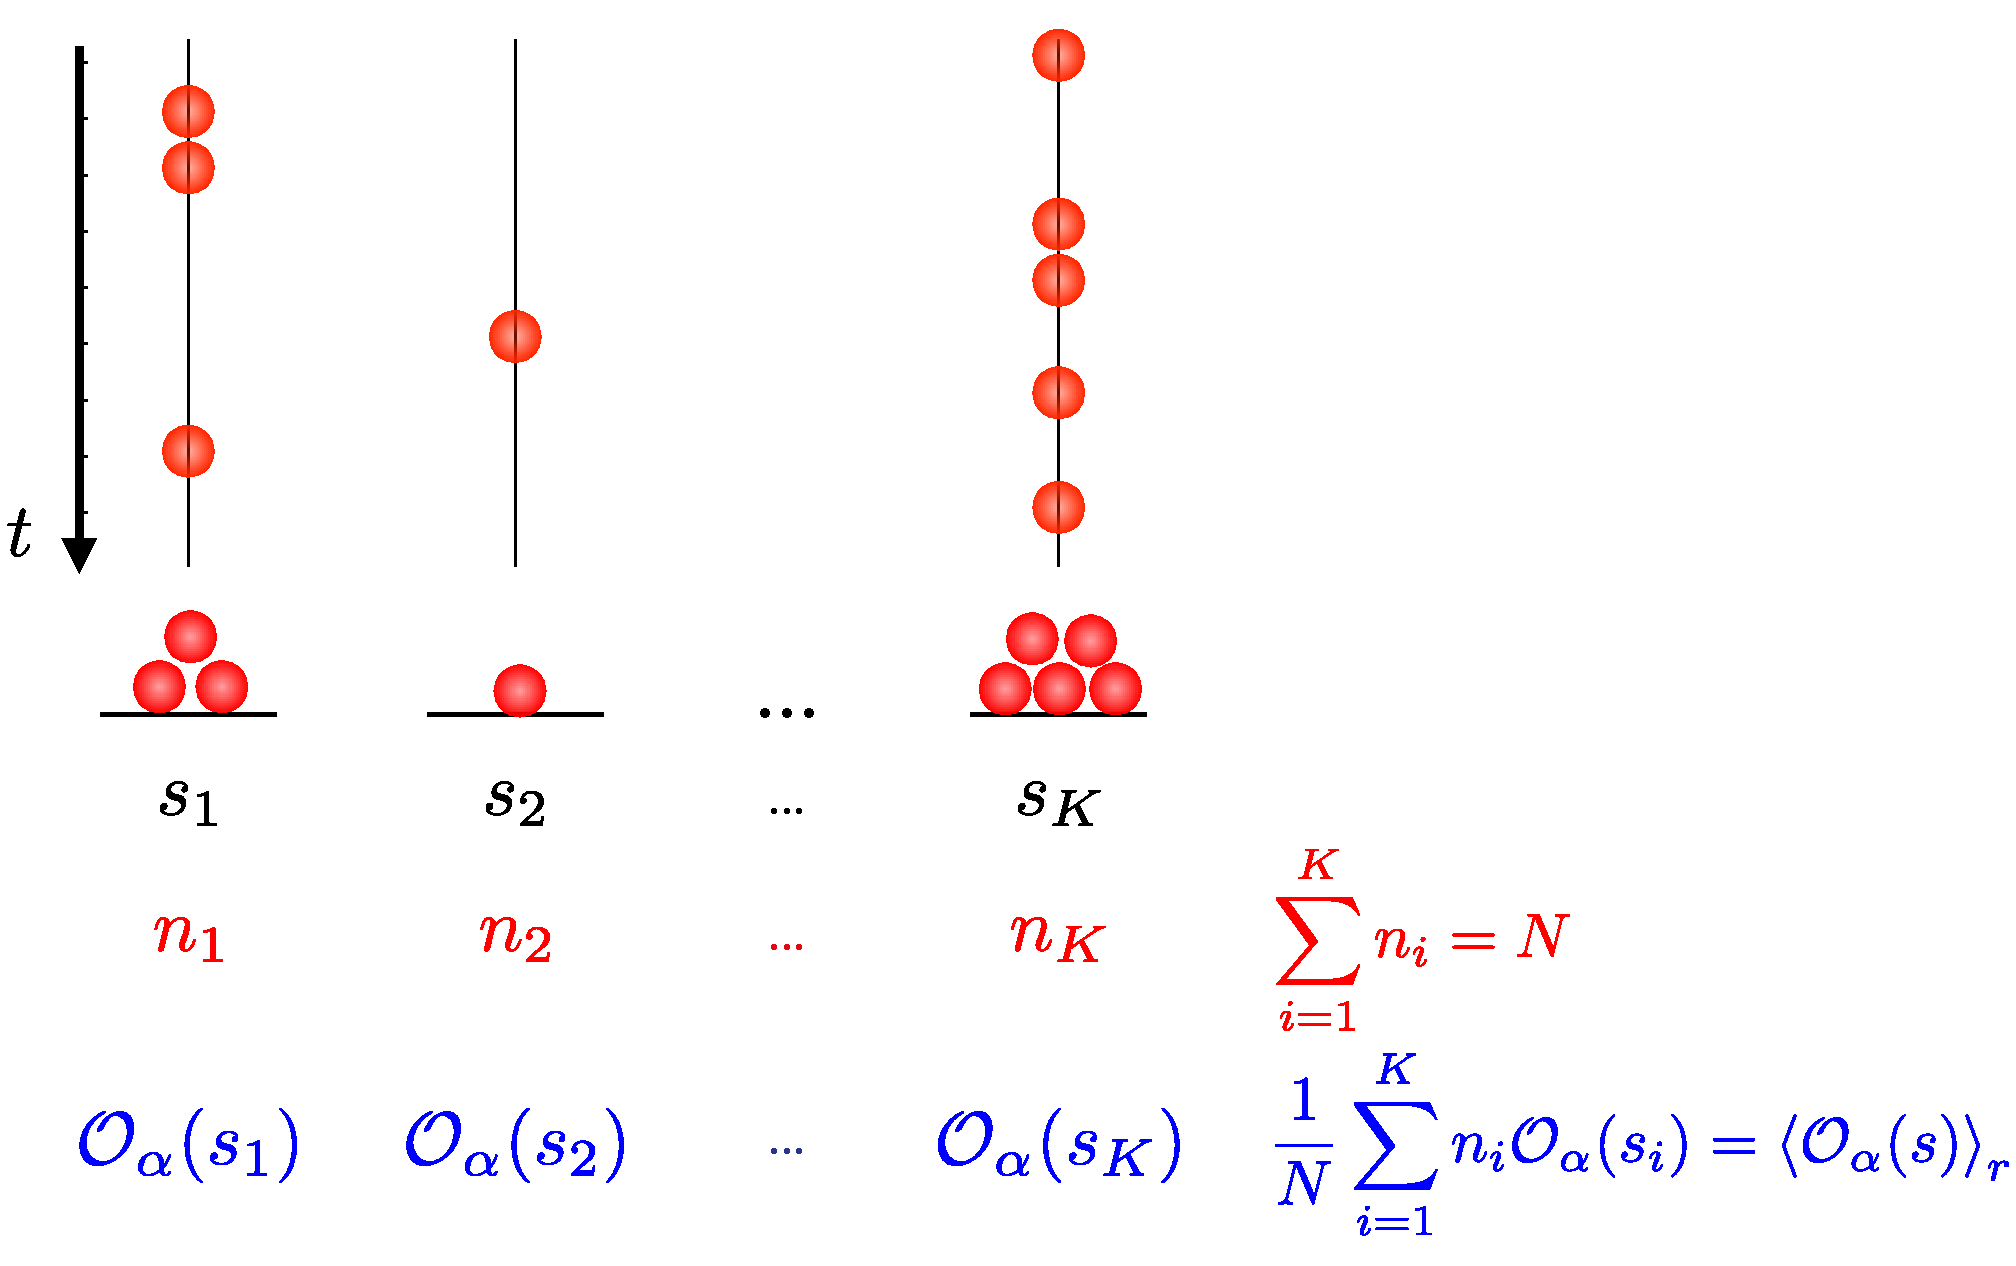
\includegraphics[width=1.0\textwidth]{figures/entropie.pdf}
\captionbf{Illustration d'un syst�me dont on veut maximiser l'entropie}{

    Le syst�me explore $K$ �tats $\{s_1,\cdots,s_K\}$ au cours du temps. Au
    bout de $N$ observations, un �tat $s_i$ a �t� observ� $n_i$ fois. � chaque
    �tat correspond un certain nombre de quantit�s $\mathcal{O}_\alpha(s_i)$,
    appel�es observables, dont seule la valeur moyenne empirique $\left\langle
    \mathcal{O}_\alpha(s)\right\rangle_r$ est connue de l'observateur.

}
\label{fig:entropie}
\efig


\subsection{Pourquoi maximiser l'entropie?}
\label{sub:pourquoi_maximiser_l_entropie_}

Le concept d'entropie remonte aux pr�misses de la physique
statistique~\cite{Jaynes1978p795}. Dans l'essence, il peut �tre compris de la
mani�re suivante. Supposons qu'un syst�me comporte $K$ �tats distincts
$\{s_1,\cdots,s_K\}$. Au cours du temps, le syst�me explore les diff�rents
�tats (fig.~\ref{fig:entropie}). Au bout de $N$ observations, chaque �tat a �t�
observ� un nombre $n_i$ de fois. La question sous-jacente au calcul de
l'entropie est la suivante : sans connaissance \apriori sur le syst�me, que
puis-je dire de ces $n_i$? Prenons l'exemple de la figure \ref{fig:entropie}.
On a certaines valeurs pour les $n_i$ ($n_1=3$, $n_2=1$, etc.), et on aimerait
savoir de combien de mani�res il est possible de r�aliser un tel ensemble de
valeurs. Notons ce nombre $\mathcal{N}(n_1,\cdots,n_K)$. Il est donn� par la
formule suivante :

\begin{align}
    \begin{split}
    \mathcal{N}(n_1,\cdots,n_K) & = \binom{N}{n_1}\binom{N-n_1}{n_2}\cdots\binom{N-\sum_{i=1}^{K-1} n_i}{n_K} \\
    & = \frac{N!}{(N-n_1)!n_1!} \times \frac{(N-n_1)!}{(N-n_1-n_2)!n_2!} \times \cdots \times \frac{(N-\sum_{i=1}^{K-1}n_i)!}{0!n_K!}
    \end{split}
\end{align}

soit en utilisant $0!=1$ :

\begin{equation}
   \mathcal{N}(n_1,\cdots,n_K) = \frac{N!}{n_1!n_2!\cdots n_K!} 
\end{equation}    

Il convient alors de s'int�resser au logarithme de cette quantit�. En effet, dans le cas o� les nombres d'observation sont grands, ceux-ci se formulent simplement gr�ce � la formule de Stirling :

\begin{equation}
    \log(n!) \xrightarrow[n\to\infty]{} n\log(n)-n
\end{equation}

On peut alors �crire

\begin{align}
    \begin{split}
   \log\mathcal{N}(n_1,\cdots,n_K) & = N\log(N) - N - \sum_{i=1}^K \left(n_i\log(n_i) -n_i\right) \\ 
   & = \sum_{i=1}^K n_i\log(\frac{N}{n_i}) \\ 
   & = -N \sum_{i=1}^K \frac{n_i}{N}\log(\frac{n_i}{N})
   \end{split}
\end{align}

On note l'apparition des probabilit�s empiriques $f(s_i)=\frac{n_i}{N}$ d'observer
l'�tat $s_i$, qui tendent asymptotiquement (dans la limite \og thermodynamique \fg
$n \to \infty$) vers les \og vraies \fg probabilit�s $P(s_i)$. L'entropie est d�finie dans cette limite comme �tant �gale � $1/N\log\mathcal{N}(n_1,\cdots,n_K)$, soit

\begin{equation}
   \label{eq-entropy}
   \boxed{
   S[P] = - \sum_{\left\{ s \right\}}P(s) \log P(s)
   }
\end{equation}

o� $\{s\} = \{s_1,\cdots,s_K\}$. L'id�e est alors la suivante : nous souhaitons
savoir quels �tats le syst�me a le plus probablement visit� au cours de ses $N$
transitions. Sans connaissance \apriori sur le syst�me, il est plus probable
que les nombres $(n_1,\cdots,n_K)$ obtenus soit ceux qui sont r�alis�s le plus
souvent, \cad ceux qui maximisent la quantit� $\mathcal{N}(n_1,\cdots,n_K)$, et
donc au final l'entropie. Par ailleurs, les fluctuations relatives des
quantit�s $n_i$ sont de l'ordre de $1/\sqrt{n_i}$~\cite{sethna2006statistical}.
Ainsi, la solution de maximum d'entropie domine largement les autres solutions
possibles dans la limite thermodynamique.

% subsection pourquoi_maximiser_l_entropie_ (end)

\subsection{Maximisation de l'entropie sous contraintes}
\label{sub:maximisation_de_l_entropie_sous_contraintes}

Notons $\mathcal{O}_\al(s)$ une quantit� attach�e � $s$
(fig.~\ref{fig:entropie}). En thermodynamique, une telle quantit� correspond
par exemple � l'�nergie d'un �tat. L'observateur n'a acc�s qu'aux valeurs
moyennes de telles quantit�s sous-jacentes. Les valeurs moyennes empiriques
calcul�es avec les fr�quences $f(s)$ doivent donc �tre compatibles avec les
valeurs moyennes calcul�es avec la distribution de probabilit� $P(s)$ :

\begin{equation}
   \label{eq:constraints}
   \sum_{\{s\}} P(s) \mathcal{O}_\al(s) = \sum_{\{s\}}f(s) \mathcal{O}_\al(s)
\end{equation}

Nous souhaiterions maintenant conna�tre la distribution $P(s)$ la moins biais�e
(i.e de maximum d'entropie) sachant les contraintes de l'�q.
\ref{eq:constraints} impos�es par l'observation des donn�es. Ce probl�me
revient � maximiser le Lagrangien suivant :

\begin{equation}
   \mathcal{L}  =  - \sum_{\{ s \}} P(s) \log P(s) + \lambda \left(\sum_{\{ s \}}
   P(s) -1\right)  +  \sum_\al \beta_\al \sum_{\{s\}} \left( P(s) - f(s) \right) \mathcal{O}_\al(s) 
\end{equation}

o� les param�tres $\lambda$ et $\beta_\al$ sont les multiplicateurs de Lagrange
correspondant respectivement � la contrainte de normalisation de la
distribution de probabilit� et aux correspondances des valeurs moyennes de
l'�q. \ref{eq:constraints}.  La maximisation de ce Lagrangien est obtenue en
annulant la d�riv�e fonctionnelle par rapport � la distribution de probabilit�
$P(s)$ :

\begin{equation}
   \frac{\delta \mathcal{L}}{\delta  P(s)}   =  0  
   = - \ln P(s) - 1  + \lambda  
   +  \sum_{\al} \beta_\al \mathcal{O}_\al(s)
\end{equation}

En utilisant la normalisation des probabilit�s, il est possible de trouver
$\lambda$, et la solution se met finalement sous la forme 

\begin{equation}
    \label{eq:boltzmann}
    \boxed{
        P(s) = \frac{1}{\mathcal{Z}} e^{-\mathcal{H}(s)}
    }
\end{equation}

o� $\mathcal{H}$ est l'Hamiltonien du syst�me :

\begin{equation}
   \mathcal{H} = \sum_\al \beta_\al\mathcal{O}_\al(s)
\end{equation}

et $\mathcal{Z}$ est la fonction de partition permettant la normalisation de la
distribution $P$ :

\begin{equation}
   \mathcal{Z}=\sum_{\{s\}} \exp[- \mathcal{H}(s)].
\end{equation}


\Remarque{

    \footnotesize{
        Il est possible de montrer que la maximisation de l'entropie, partant des
        contraintes sur les valeurs moyennes pour en arriver � une forme exponentielle
        de la distribution de probabilit�, est le contrepoint d'une maximisation de la
        vraisemblance partant d'une forme exponentielle pour en arriver aux m�mes
        conditions sur les valeurs
        moyennes~\cite{grendar2001minimax,jaynes1982rationale}.
    }

}

% subsection maximisation_de_l_entropie_sous_contraintes (end)

\subsection{Application aux sites de fixation}
\label{sub:application_aux_sites_de_fixation}

\subsubsection{Corr�lation � un point : le mod�le PWM}
\label{ssub:corr_lation_un_point_le_mod_le_pwm}

Dans notre cas, un �tat $s$ correspond � une s�quence d'ADN appartenant
� l'ensemble $\left\{ s \right\}$ des sites de fixation d'un \tf. Consid�rons
maintenant l'observable quantifiant la pr�sence du nucl�otide $a$ � la position
$i$ d'un site :

\begin{equation}
    \mathcal{O}_{i,a}(s) = \delta(s_i,a)
\end{equation}


o� $\delta$ est la fonction de Kronecker qui vaut $1$ lorsque le nucl�otide
� la position $i$ du site $s_i$ est $a$ et $0$ sinon. De cette d�finition il suit que la valeur moyenne sur les fr�quences empiriques


\begin{equation}
    \label{eq:onepoint}
    \sum_{\{s\}} f(s) \mathcal{O}_{i,a}(s) = f_{i,a}
\end{equation}

se r�duit � la fr�quence du nucl�otide $a$ � la position $i$. Notons $h_i(a)$
le multiplicateur de Lagrange correspondant et $\mathcal{A} = \{A,C,G,T\}$. On trouve alors

\begin{align}
    \begin{split}
    \mathcal{H}(s) & = \sum_{i=1}^L \sum_{a \in \mathcal{A}} h_i(a) \delta(s_i,a)\\
     & = \sum_{i=1}^L h_{i}(s_i)
    \end{split}
\end{align}

Les diff�rentes positions �tant ind�pendantes, la fonction de partition
$\mathcal{Z}$ peut par ailleurs se scinder en fonctions de partitions par
position $\mathcal{Z}=\prod_{i=1}^L\mathcal{Z}_i$. On obtient au final

\begin{equation}
    P(s) = \frac{1}{\mathcal{Z}} e^{-\sum\limits_{i=1}^L h_i(s_i)} = \prod_{i=1}^L \frac{e^{-h_i(s_i)}}{\mathcal{Z}_i}
\end{equation}

On retrouve le mod�le PWM introduit dans l'�q.~\ref{eq:boltzmann}.



% subsubsection corr_lation_un_point_le_mod_le_pwm (end)

\subsubsection{Corr�lations � deux points : le mod�le de Potts}
\label{ssub:corr_lations_deux_points_le_mod_le_de_potts}


Il est maintenant relativement direct de complexifier le mod�le en ajoutant
l'observation des couples d'interaction au sein des sites de fixation :

\begin{equation}
    \mathcal{O}_{i,a,j,b}(s) = \delta(s_i,a)\delta(s_j,b)
\end{equation}

La corr�lation � deux points entre le nucl�otide $a$ en position $i$ et $b$ en
position $j$ s'�crit donc 

\begin{equation}
    \label{eq:twopoints}
    \sum_{\{s\}} f(s) \mathcal{O}_{i,a,j,b}(s) = f_{i,a,j,b}
\end{equation}

o� $f_{i,a,j,b}$ est la fr�quence empirique d'observation de la paire de
nucl�otide $(a,b)$ aux positions $(i,j)$. Notons $J_{i,j}(a,b)$ le
multiplicateur de Lagrange correspondant. L'Hamiltonien sous les contraintes
impos�es par les �quations \ref{eq:onepoint} et \ref{eq:twopoints} s'�crit :


\begin{align}
    \begin{split}
    \mathcal{H}(s) & = \sum_{i=1}^L \sum_{a \in \mathcal{A}} h_i(a) \delta(s_i,a) + \sum_{i=1}^{L-1} \sum_{j>i} \sum_{a \in \mathcal{A}} \sum_{b \in \mathcal{A}} J_{i,j}(a,b) \delta(s_i,a)\delta(s_j,b)\\
    & = \sum_{i=1}^L h_{i}(s_i) + \sum_{i=1}^{L-1}\sum_{j>i} J_{i,j}(s_i,s_j)
\end{split}
\end{align}

Le mod�le de maximum d'entropie est finalement

\begin{equation}
    \boxed{
    P(s) = \frac{1}{\mathcal{Z}} e^{-\sum\limits_{i=1}^L h_i(s_i)-\sum\limits_{i=1}^{L-1} \sum\limits_{j>i} J_{i,j}(s_i,s_j)} 
}
\end{equation}

On reconna�t le mod�le de Potts inhomog�ne de champs magn�tiques locaux $h_i$
et de termes d'interaction $J_{i,j}$~\cite{baxter2007exactly}.


% subsubsection corr_lations_deux_points_le_mod_le_de_potts (end)

% subsection application_aux_sites_de_fixation (end)


\section{Article} 
\label{sec:article}

Cet article d�crit l'analyse de donn�es de fixation \invivo � grande �chelle
pour plusieurs TFs drosophiles et mammif�res. Diff�rents mod�les sont compar�s,
incluant ou non des d�pendances : un mod�le PWM, un mod�le de m�lange de PWMs,
et un mod�le de Potts.


\includepdf[pages=-]{articles/maxent-arxiv}

% section article (end)


\section{Analyse thermodynamique des mod�les ind�pendant et avec couplages} 
\label{sec:analyse_thermodynamique_des_mod_les_ind_pendant_et_avec_couplages}


\subsection{Chaleur sp�cifique}
\label{sub:chaleur_sp_cifique}


En plus des r�sultats pr�sent�s dans l'article, nous nous sommes int�ress�s
� une quantit� classique de la thermodynamique : la chaleur sp�cifique ou
capacit� calorifique. Consid�rons un mod�le d�crit par la statistique de
Boltzmann � la temp�rature inverse $\beta=1/T$ (on omet la constante de
Boltzmann $k$ en l'int�grant � l'�nergie):

\begin{equation}
    \label{eq:boltzmann_with_beta}
    P(s) = \frac{1}{\mathcal{Z}} e^{-\beta E(s)}
\end{equation}

Le cas de l'�quation \ref{eq:boltzmann} correspond au cas particulier $\beta=1$
(\cad que le param�tre $\beta$ est incorpor� dans les diff�rents
$\beta_\alpha$). Nous voulons voir comment l'amplification ou la diminution
globale de l'�cart entre les �nergies affecte la possibilit� du syst�me
d'explorer les diff�rents �tats $s$ possibles. � temp�rature nulle ($T\to0 $ ou
$\beta \to \infty$), le syst�me reste dans le niveau fondamental de minimum
d'�nergie, alors qu'� des temp�ratures non nulles le syst�me � l'�nergie $E_0$
transite vers un �tat d'�nergie sup�rieure $E_1$ avec une probabilit�
$\exp\left(-\beta (E_1-E_0)\right)$. Lorsqu'un paysage �nerg�tique est compos�
de plusieurs puits d'�nergie avec des barri�res importantes, on s'attend
� avoir une (ou plusieurs) temp�ratures critiques pour lesquelles de fortes
diff�rences d'�nergie deviennent franchissables. L'�nergie moyenne peut alors
�tre significativement affect�e, sautant soudainement � une nouvelle valeur du
fait des poids des nouveaux �tats explor�s. 

La chaleur sp�cifique permet de caract�riser ces sauts soudains d'�nergie
moyenne lors de la variation de la temp�rature, caract�risant des transitions
de phase. Elle mesure simplement la variation d'�nergie moyenne r�sultant d'une variation de temp�rature :

\begin{equation}
    C(T) = \frac{d\langle E \rangle}{dT}
\end{equation}

or en utilisant 

\begin{equation}
    \langle E \rangle = \sum_{\{s\}} E(s) \frac{e^{-\beta E(s)}}{\mathcal{Z}}
\end{equation}

on trouve que

\begin{align}
    \begin{split}
        \frac{d\langle E \rangle}{dT} & = - \beta^2 \frac{d\langle E \rangle}{d\beta} \\
        & = \beta^2 \left[\sum_{\{s\}} E(s) \left( -E(s) e^{-\beta E(s)} \right)\frac{1}{\mathcal{Z}} + \sum_{\{s\}} E(s) e^{-\beta(E(s))} \left(-\frac{d\mathcal{Z}}{d\beta} \frac{1}{\mathcal{Z}^2}\right)\right] \\
    & = \beta^2 \left[ \langle {E}^2 \rangle - {\langle E \rangle}^2 \right]
    \end{split}
\end{align}

Ainsi, la chaleur sp�cifique $C(T)$ est directement accessible en regardant les
corr�lations de l'�nergie sur l'ensemble des �tats du syst�me. Nous avons
calcul� sa variation en fonction de la temp�rature pour les mod�les ind�pendant
et avec d�pendances obtenus pour les diff�rents TFs �tudi�s. L'introduction de
la temp�rature se faire de mani�re fictive en multipliant les �nergies par
$\beta$, afin de se placer dans le cadre de l'�quation
\ref{eq:boltzmann_with_beta}. Les r�sultats sont montr�s en
figure~\ref{fig:maxent/specific_heat} (mod�le ind�pendant en bleu, mod�le de
Potts en rouge). On observe pour la plupart des facteurs l'existence de deux
pics de chaleur sp�cifique pour des temp�ratures de l'ordre de $\sim10^{-1}$ et
$\sim 5$ (par exemple, $0.4$ et $2.8$ pour le mod�le ind�pendant de Twist). Il
y a de l�g�res variations entre les deux mod�les : notamment, le premier pic
semble renforc� dans plusieurs cas. N�anmoins, le nombre de transitions de
phase (ou de pics) reste le m�me.

\bfig
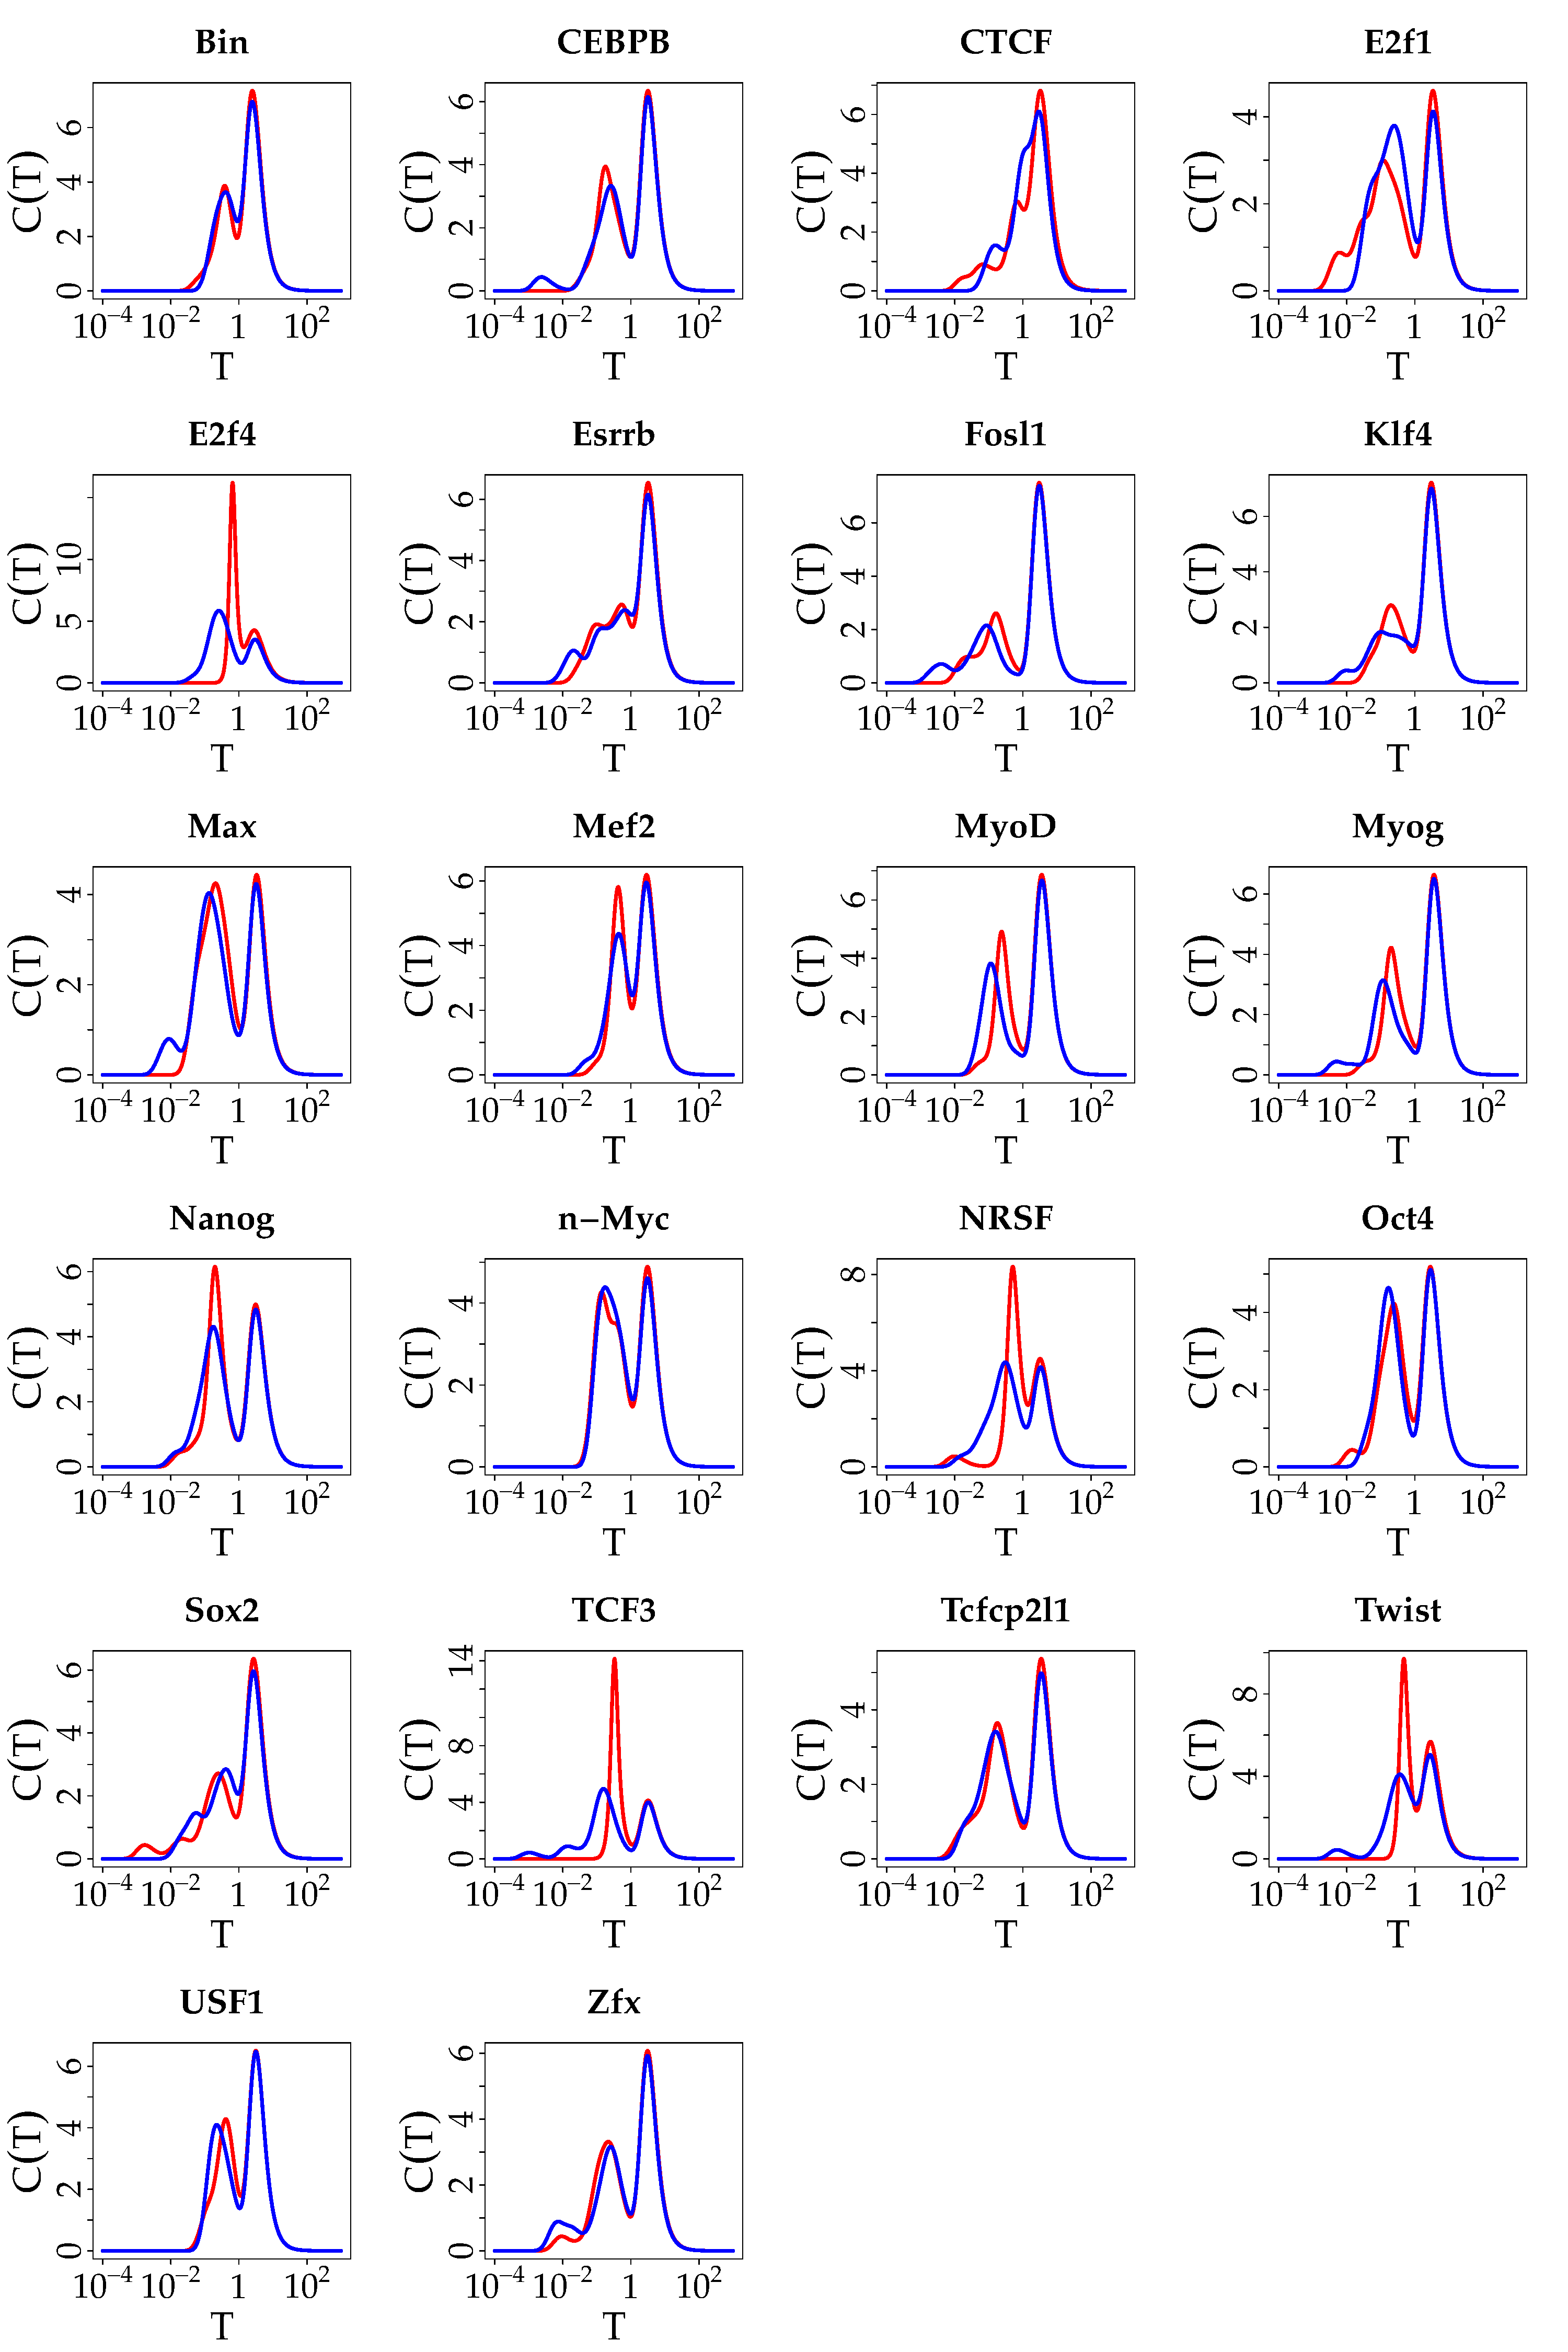
\includegraphics[width=.8\textwidth]{figures/maxent/specific_heat.pdf}
\captionbf{Chaleur sp�cifique pour diff�rents TFs}{

    La chaleur sp�cifique (l'�quivalent de la capacit� calorifique en
    thermodynamique) $C(T)=d\langle E\rangle/dT$ est trac�e en fonction de la
    temp�rature $kT$ (�chelle logarithmique) pour les diff�rents TFs
    consid�r�s. Le mod�le ind�pendant (bleu) et le mod�le de Potts avec
    interactions (rouge) sont comparables dans la plupart des cas.

}
\label{fig:maxent/specific_heat}
\efig

% subsection chaleur_sp_cifique (end)

\subsection{Lien avec les valeurs des champs et des couplages}
\label{sub:lien_avec_les_valeurs_des_champs_et_des_couplages}

Afin de comprendre l'existence des pics de chaleur sp�cifique et les �nergies
(temp�ratures) associ�es, il faut revenir aux mod�les d'�nergie. Dans le mod�le
ind�pendant, les champs sont simplement le logarithme naturel de la probabilit�
d'observer un nucl�otide � une position donn�e $h_i(a) = -\log P_i(a)$ (la
jauge est choisie telle que $\mathcal{Z}=1$). En valeur absolue, les champs $h$
proches de $0$ correspondent aux nucl�otides tr�s conserv�s (toujours
observ�s), les valeurs autour de $1$ correspondent � des nucl�otides �galement
observ�s ($|\log(1/4)| \sim 1.4$) et les valeurs autour de $10$ correspondent
aux nucl�otides qui ne sont jamais observ�s, au pseudocount pr�s (pour un
pseudocount de $1$ et $10^4$ s�quences, $|\log(10^{-4})| \sim 9.2$). On
retrouve ces valeurs typiques lorsque l'on regarde l'histogramme des valeurs
absolues de $h$ obtenues dans les mod�les ind�pendant des diff�rents TFs
�tudi�s (fig.~\ref{fig:histogrammes_champs}A).  On peut maintenant mieux
comprendre les pics de chaleur sp�cifique. Lorsque la temp�rature se rapproche
de $1$ (par le bas), les nucl�otides d�g�n�r�s d'�nergie $h_i\sim1$ deviennent
accessibles, augmentant significativement la valeur de l'�nergie moyenne. Puis,
lorsque la temp�rature se rapproche de $10$, les nucl�otides non observ�s
d'�nergie $h_i\sim10$ deviennent � leur tour accessibles, augmentant � nouveau
l'�nergie moyenne.

Dans le cas du mod�le de Potts (fig.~\ref{fig:histogrammes_champs}B), on
observe des interactions r�parties autour d'un mode centr� autour de $J_{i,j}
\sim 0.5$. Ceci explique sans doute le renforcement du premier pic de chaleur
sp�cifique observ� pour plusieurs TFs de la figure
\ref{fig:maxent/specific_heat} (par exemple, E$2$f$4$, NRSF, TCF$3$ ou Twist).




\bfig
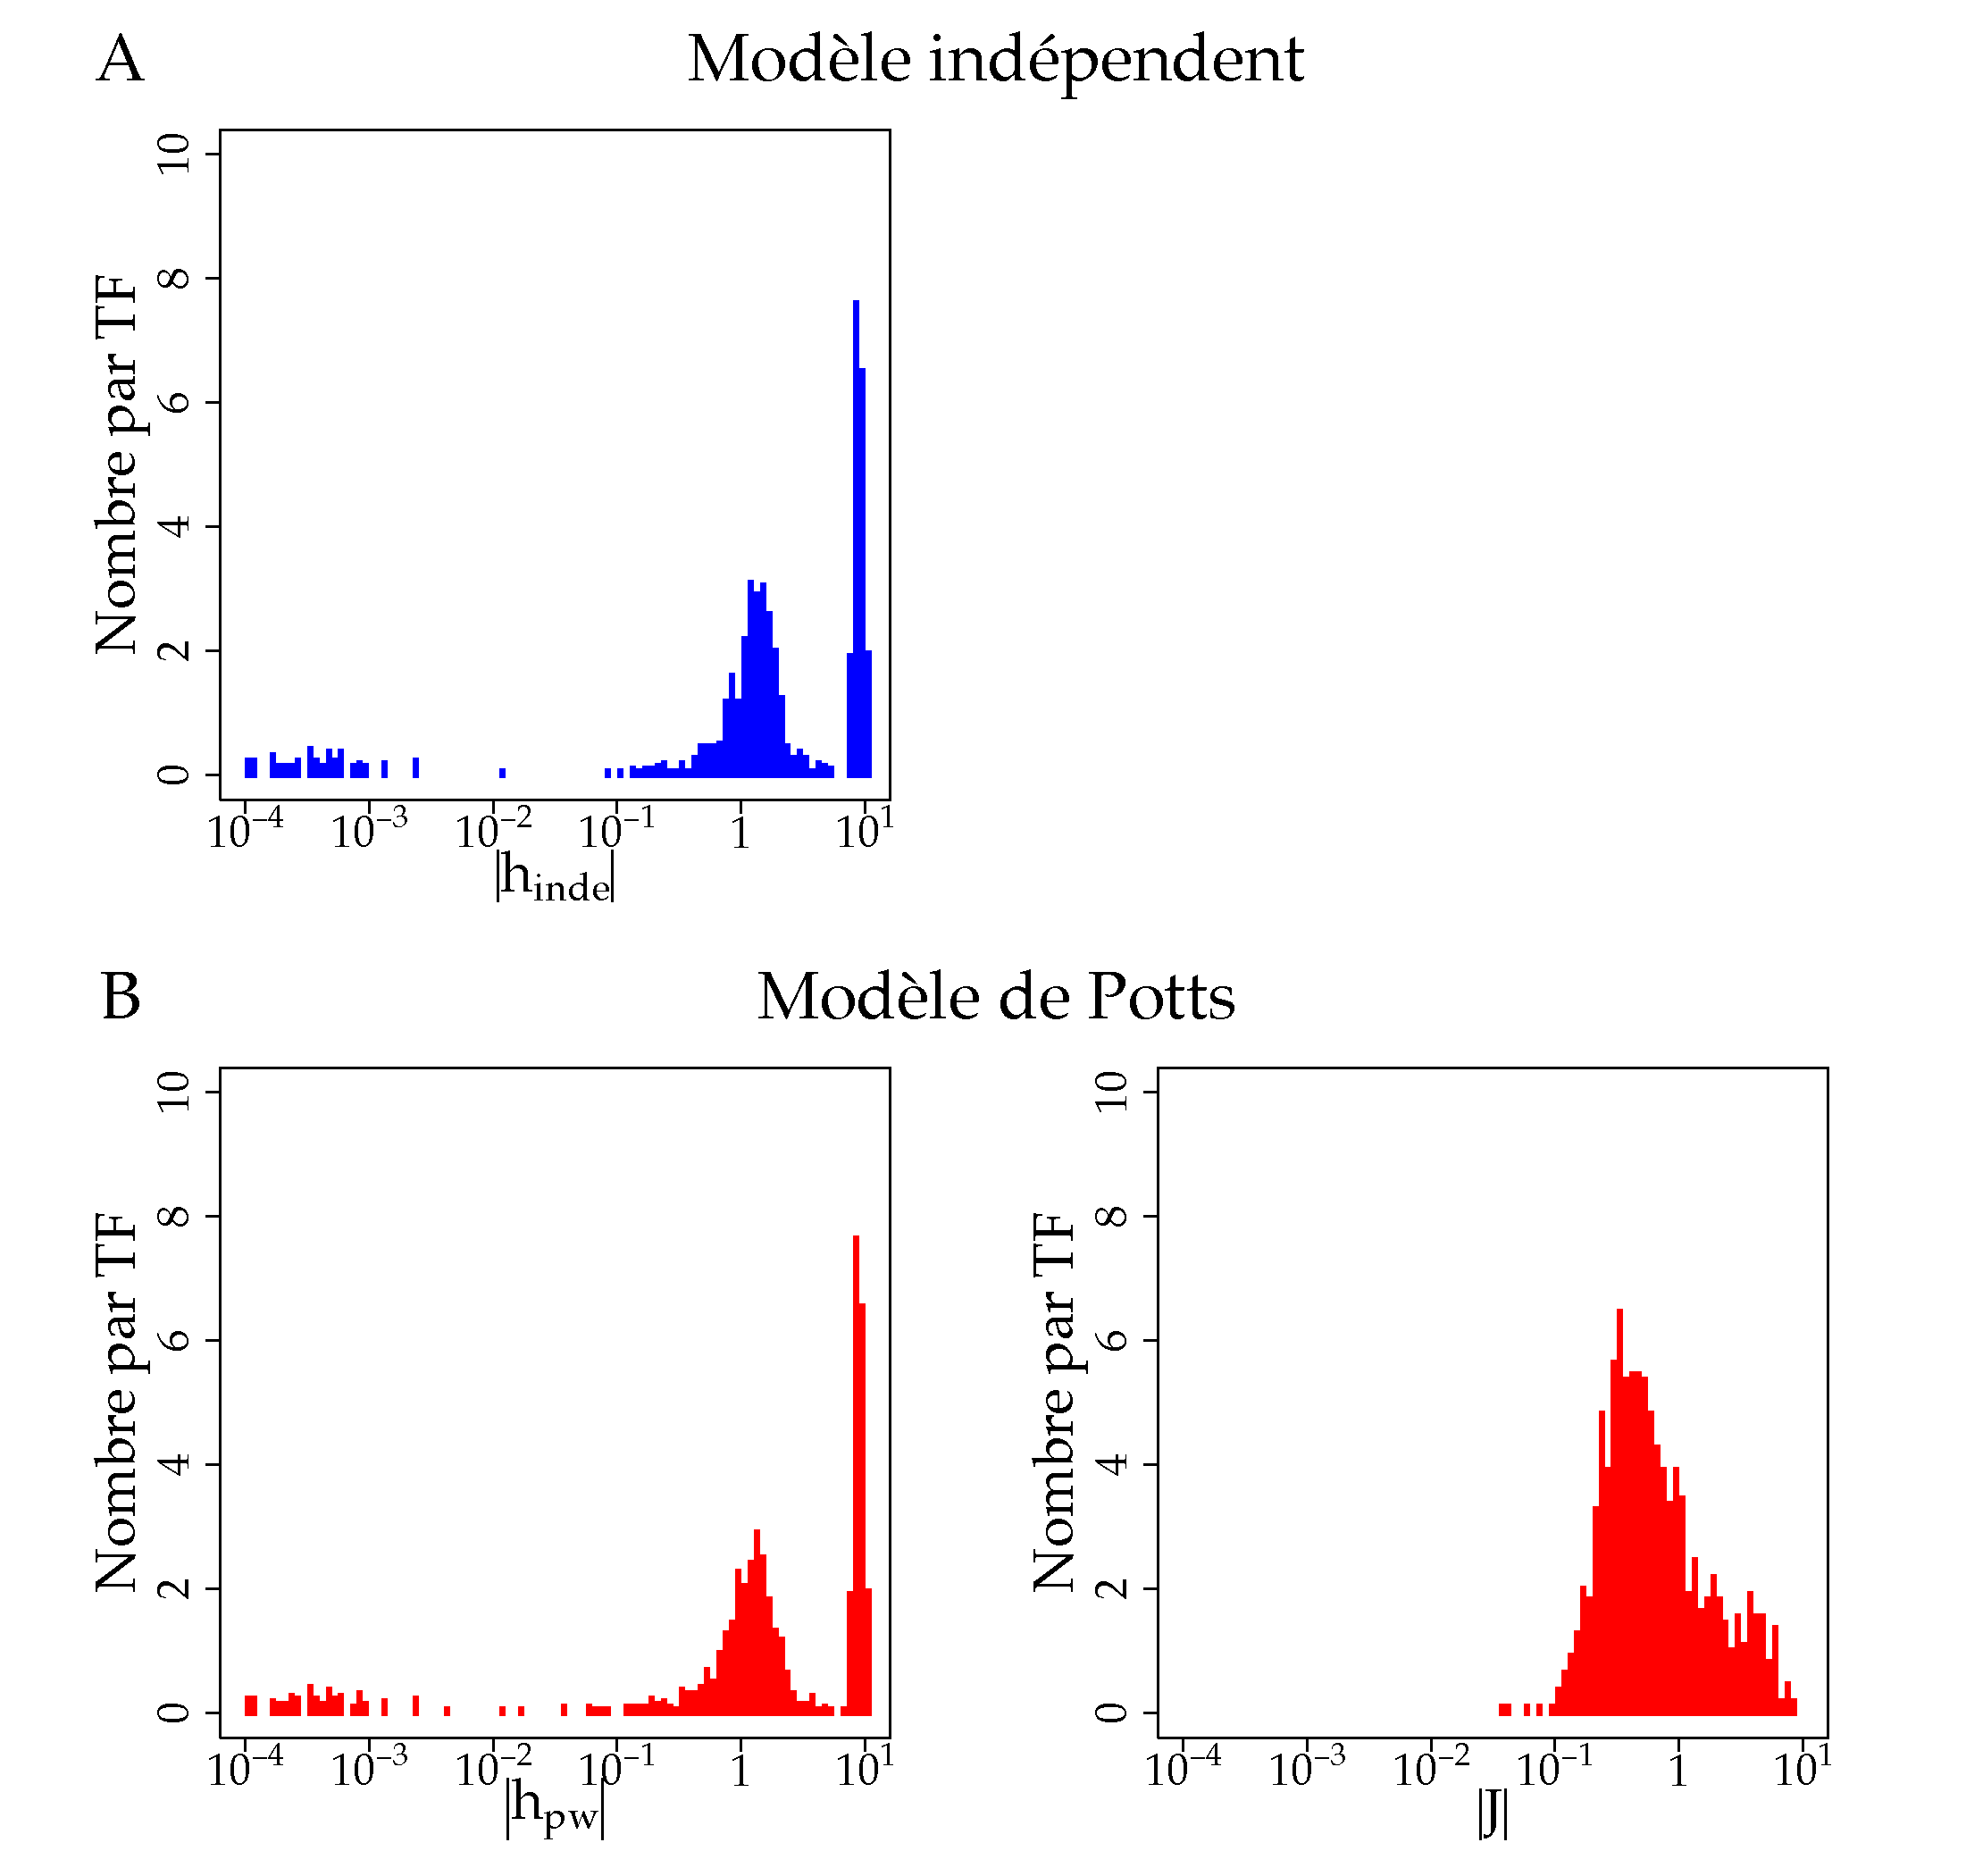
\includegraphics[width=1.\textwidth]{figures/maxent/histogrammes_champs.pdf}
\captionbf{Histogrammes des valeurs des champs $h$ et couplages $J$}{

    Histogrammes r�alis�s � partir des valeurs obtenues pour l'ensemble des
    TFs. Les champs et les couplages sont montr�s en valeur absolue sur une
    �chelle logarithmique d'espacement $0.05$, et les valeurs nulles ne sont
    pas repr�sent�es. (A) Champs $h_{inde}$ dans le mod�le ind�pendant. (B)
    Champs $h_{pw}$ et couplages $J$ dans le mod�le de Potts.

}
\label{fig:histogrammes_champs}
\efig




% subsection lien_avec_les_valeurs_des_champs_et_des_couplages (end)
\FloatBarrier

% section analyse_thermodynamique_des_mod_les_ind_pendant_et_avec_couplages (end)
\section{Conclusion et perspectives}


Nous avons analys� les d�pendances au sein des sites de fixation li�s \invivo
pour plusieurs \tfs Drosophiles et mammif�res. Nous avons compar� les
performances d'un mod�le PWM, d'un mod�le de m�lange de PWMs, et d'un mod�le de
Potts, en utilisant un crit�re bay�sien (BIC) p�nalisant les mod�les � grand
nombre de param�tres. Nous avons exhib� l'existence de corr�lations faibles
dont la prise en compte permet de significativement am�liorer la description
des donn�es, le mod�le de Potts �tant significativement sup�rieur aux deux
autres mod�les dans la plupart des cas ($22/28$). Les interactions ont �t�
�tudi�es syst�matiquement, montrant notamment une pr�pond�rance des
interactions entre plus proches voisins. Nous avons �tabli une correspondance
entre les PWMs du mod�le de m�lange et les PWMs d�crivant les sites des �tats
m�tastables du paysage �nerg�tique g�n�r� par le mod�le de Potts. Enfin, nous
avons montr� que les corr�lations pouvaient �tre group�es en patterns de
Hopfield ou \og m�moires \fg, et qu'un petit nombre �tait suffisant
� reconstruire le paysage d'interactions.
\\

Une perspective int�ressante de ce travail serait de conduire la m�me analyse
sur des donn�es grande �chelle obtenues \invitro par la m�thode
HT-SELEX~\cite{Jolma2013p3971}. Notamment, certains des facteurs que nous avons
�tudi�s \invivo sont repr�sent�s dans ces donn�es, et il serait int�ressant de
voir les diff�rences entre les deux mod�les de Potts et mod�les de m�langes
obtenus. Notamment, retrouve-t-on les m�mes corr�lations? Peut-on exhiber des
sp�cificit�s � la fixation \invivo, o� l'on s'attend � avoir des effets
provenant de diverses sources (fixation de nucl�osomes, superposition de sites
de fixations, \ldots)? Ces questions feront l'objet d'un prochain travail.



\newpage

%%%%%%%%%%%%%%%%%%%%%%%%%%%%%%%%%%%%%%%%%%%%%%%%%%%%%%%%%%%%%%%%%%%%%%%%%%%%%%%%%%%%%%%%%%
\chapter{\ChImogene} 
\label{ch:imogene}
%\adjustmtc
\minitoc
\newpage
\section*{Introduction du chapitre \thechapter}

Dans le chapitre \ref{ch:maxent}, nous avons vu comment d�crire l'interaction
TF-ADN lorsque des sites de fixation sont connus. Dans ce chapitre, nous
adoptons une d�marche plus g�n�rale. Nous connaissons l'activit� de r�gulation
d'un certain nombre de CRMs, et nous souhaitons savoir quels TFs s'y fixent
(recherche de motifs), et si le g�nome contient d'autres CRMs avec la m�me
activit� (recherche de modules). Un algorithme permettant pr�cis�ment de
r�aliser ces �tapes a �t� d�velopp� pr�c�demment par Herv� Rouault et appliqu�
au cas de la diff�renciation des organes sensoriels de la
Drosophile~\cite{Rouault2010p327}. Nous pr�sentons ici l'extension de cet
algorithme au cas des mammif�res, ainsi que son utilisation comme outil de
classification de CRMs associ�s � diff�rentes r�gulations.


\section{Recherche de motifs dans des CRMs} 
\label{sec:recherche_de_motifs_dans_des_crms}

Avant de rentrer dans le d�tail d'Imogene, nous pr�sentons les m�thodes
existantes de recherche de motifs dans des CRMs. Le probl�me g�n�ral est le
suivant : �tant donn�es des CRMs conduisant � une m�me r�gulation, peut-on
construire des mod�les de sites de fixation qui \og expliquent \fg cette
co-r�gulation, \cad qui pr�disent l'existence de sites sur les CRMs mais
pas sur des s�quences ne participant pas � la cor�gulation? L'une des
difficult�s majeures ici est que la position des sites dans les s�quences n'est
pas connue.

\subsection{Apprentissage par esp�rance-maximisation}
\label{sub:algorithmes_de_type_esp_rance_maximisation}

L'une des premi�res approches de ce probl�me a �t� celle de
MEME~\cite{Bailey1994fk}, un algorithme bas� sur la m�thode
d'esp�rance-maximisation ou EM (\textit{expectation maximization}) utilis�e
pr�c�demment dans ce cadre par \citet{Lawrence1990uq}. Cet algorithme se base
sur une approche g�n�rative pour d�crire les processus probabilistes qui ont
permis la g�n�ration des s�quences CRMs (fig.~\ref{fig:d_haeseleer-MEME}). 

\bfig
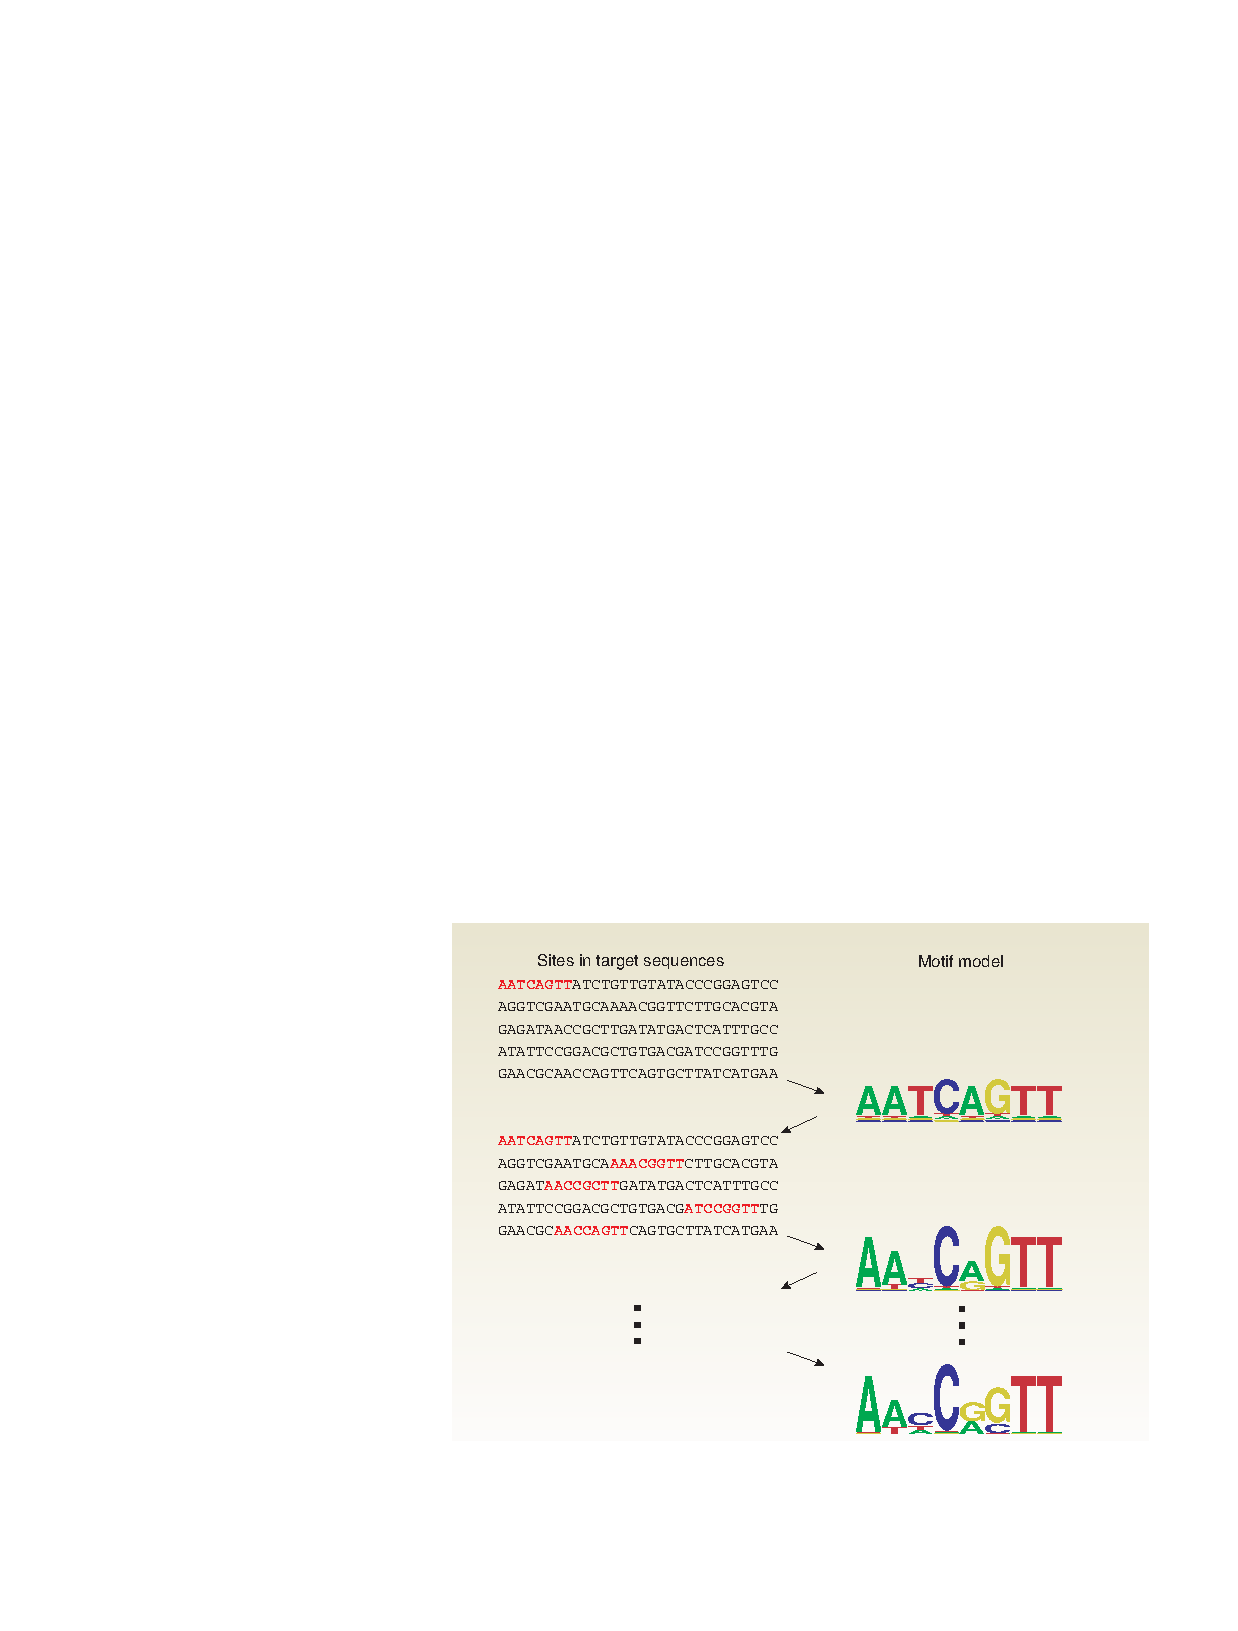
\includegraphics[width=0.8\textwidth]{figures/d_haeseleer-MEME.pdf}
\captionbf{Illustration de l'approche esp�rance-maximisation}{

Figure tir�e de \cite{Dhaeseleer2006kx} d�crivant l'approche EM. Un premier
mod�le de motif est construit � partir d'un site initial. Ce mod�le permet de
pond�rer l'ensemble de sites sur les s�quences (�tape E). En rouge sont montr�s
les meilleurs sites pour chaque s�quence. En utilisant ces poids, il est
possible de construire un mod�le de vraisemblance maximale (�tape M). La
m�thode originale de \citet{Lawrence1990uq} fait l'hypoth�se qu'il
y a exactement un site de fixation par s�quence, condition qui est rel�ch�e par
MEME. 

} \label{fig:d_haeseleer-MEME} \efig


\subsubsection{Vraisemblance d'une s�quence}
\label{ssub:vraisemblance_d_une_s_quence}


Notons $S=\{S_1,\cdots,S_L\}$ une s�quence de taille $L$\footnote{On concat�ne
les deux brins d'ADN dans cette s�quence. On suppose en effet qu'ils
participent �quiprobablement � la fixation. Ainsi la s�quence g�nomique double
brins est de longueur $L/2$.}. Supposons qu'il y a exactement un site de
r�gulation par CRM. C'est l'approche de \citet{Lawrence1990uq}, et cette
condition est rel�ch�e par MEME, qui autorise l'utilisateur � pr�ciser un
nombre moyen de sites par s�quence. La probabilit� que la s�quence poss�de un
site de taille $K$ � la position $i$ �tant donn� le mod�le $\mathcal{M}$
s'�crit 

\begin{equation}
    \label{eq:prob-sequence-oops}
    P(S|i,\mathcal{M}) = P_0(S_{1,i-1})\times P(S_{i,i+K-1} | \mathcal{M})\times P_0(S_{K,L})
\end{equation}

o� $S_{i,j}$ d�note la s�quence entre les positions $i$ et $j$ incluses,
$P(S_{i,i+K-1}|\mathcal{M})$ est la probabilit� de g�n�rer la s�quence de
taille $K$ d�butant � la position $i$ avec le mod�le $\mathcal{M}$ (voir
section \ref{sec:mod_les_pour_d_crire_les_corr_lations}), et $P_0(s)$ est la
probabilit� neutre ou \textit{background} de g�n�rer la s�quence $s$. Cette
derni�re est g�n�ralement prise comme �tant une cha�ne de Markov
$\mathcal{P}_k$ d'ordre $k$ petit ($0$ ou $1$) :

\begin{equation}
    P_0(S_{i,j}) = \prod_{l=i}^{j} \mathcal{P}_k(S_l | S_{l-k,l-1})
\end{equation}

Ainsi, l'�quation \ref{eq:prob-sequence-oops} d�crit la probabilit� de g�n�rer
la s�quence $S$ avec le mod�le \textit{background}, sauf � la position $i$ o�
un site est g�n�r� avec le mod�le de fixation $\mathcal{M}$. La probabilit� de g�n�rer la s�quence s'obtient finalement en sommant sur les positions pond�r�es par la probabilit� \apriori $P(i)$ que le site soit � la position $i$ :

\begin{equation}
    P(S|\mathcal{M}) = \sum_{i=1}^{L-K+1} P(i) P(S|i,\mathcal{M})
\end{equation}

Cette probabilit� est g�n�ralement prise uniforme, mais on peut y incorporer
certaines informations \apriori, comme le nombre de \textit{reads} d'une
exp�rience de \chipseq par exemple.

% subsubsection vraisemblance_d_une_s_quence (end)

\subsubsection{Apprentissage du mod�le}
\label{ssub:apprentissage_du_mod_le}


Maintenant que nous savons exprimer la vraisemblance d'une s�quence r�gul�e par
le motif $\mathcal{M}$, nous pouvons apprendre le meilleur mod�le possible
l'ayant g�n�r�e : c'est la maximisation de la vraisemblance. Soit un ensemble
de s�quences $\mathcal{S}$ constitu� de $M$ s�quences co-r�gul�es
$S[1],\cdots,S[M]$.  Ces s�quences �tant suppos�es ind�pendantes, la
vraisemblance que ces donn�es soient g�n�r�es par un mod�le $\mathcal{M}$ est
le produit sur les s�quences de la quantit� $P(S[m]|\mathcal{M})$. Il est plus
utile dans ce cas de regarder la log-vraisemblance, s'�crivant alors comme une
somme :

\begin{equation}
    l(\mathcal{S} | \mathcal{M}) = \sum_{m=1}^M \log P(S[m] | \mathcal{M})
\end{equation}

Nous d�sirons obtenir le mod�le $\mathcal{M}$ maximisant cette quantit�
\footnote{ La distribution \textit{background} est suppos�e fix�e (par exemple
la cha�ne de Markov peut �tre apprise sur un grand nombre de s�quences
interg�niques non codantes).  }.  Cependant, nous ne connaissons pas les
positions exactes des sites, qui sont des \og variables cach�es \fg et il
n'existe pas de m�thode d'estimation simple permettant de r�soudre ce probl�me.
C'est � ce stade qu'intervient la m�thode Esp�rance-Maximisation
(EM)~\cite{dempster1977maximum}. L'algorithme EM est une m�thode it�rative qui
part d'un mod�le initial $\mathcal{M}^0$, permettant de calculer les poids des
positions dans les s�quences (�tape E d'esp�rance), puis estime le meilleur
mod�le $\mathcal{M}^1$ �tant donn�es ces poids (�tape M de maximisation).
L'it�ration a lieu jusqu'� convergence vers un maximum local. 


Notons $\mathcal{M}^t$ le mod�le � l'it�ration $t$. La probabilit� qu'un site
� la position $i$ dans la s�quence $S[i]$ soit un site de fixation s'�crit $P(i
| S[m], \mathcal{M}^t)$. On d�finit la log-vraisemblance moyenne d'un mod�le
$\mathcal{M}$ � l'it�ration $t$ par :

\begin{equation}
    \label{eq:loglikeli-full}
    Q(\mathcal{M}|\mathcal{M}_t,\mathcal{S}) = \sum_m \sum_i P(i | S[m],
    \mathcal{M}^t) \log P(\mathcal{S},i|\mathcal{M})
\end{equation}

Le mod�le suivant $\mathcal{M}^{t+1}$ est celui qui maximise cette quantit� :

\begin{equation}
    \mathcal{M}^{t+1} = \underset{\mathcal{M}}{\text{argmax}} Q(\mathcal{M}|\mathcal{M}_t,\mathcal{S})
\end{equation}


L'�quation \ref{eq:loglikeli-full} se scinde en une partie d�pend de
$\mathcal{M}$ et une partie \textit{background} qui n'en d�pend pas (eq.
\ref{eq:prob-sequence-oops}), que l'on peut dont ignorer pour ce qui est de la
maximisation. Ainsi, le mod�le $\mathcal{M}$ maximise la quantit� suivante :

\begin{equation}
    Q(\mathcal{M}|\mathcal{M}_t,\mathcal{S}) = \sum_m \sum_i P(i | S[m],
    \mathcal{M}^t) \log P(S_{i,i+K-1}|\mathcal{M})
\end{equation}

Chaque $K$-mer des s�quences de $\mathcal{S}$ est donc pris en compte dans
l'apprentissage en proportion de la croyance courante $P(i | S[m],
\mathcal{M}^t)$ que c'est un site de fixation. 

Pour r�sumer on a deux �tapes:

\begin{itemize}
        

    \item[$\bullet$] �tape E : utiliser $\mathcal{M}^t$ pour attribuer un poids � chaque
        $K$-mer des s�quences

    \item[$\bullet$] �tape M : apprendre $\mathcal{M}^{t+1}$ qui a la plus grande
        vraisemblance de g�n�rer les donn�es pond�r�es par $\mathcal{M}^t$.

\end{itemize}

Reste le probl�me de choisir un mod�le initial ad�quat pour ne pas converger
vers un maximum de vraisemblance local. MEME adopte pour cela une approche
semi-exhaustive. Les diff�rents $K$-mers possibles des s�quences
d'apprentissage sont successivement utilis�s pour g�n�rer un mod�le initial.
L'algorithme EM est it�r� une fois, et le mod�le de plus grande probabilit� est
finalement gard� come motif initial pour une it�ration compl�te.



% subsubsection apprentissage_du_mod_le (end)


% subsection algorithmes_de_type_esp_rance_maximisation (end)

% section recherche_de_motifs_dans_des_crms (end)


\subsection{Incorporation de l'information phylog�n�tique}
\label{sub:incorporation_de_l_information_phylog_n_tique}



% subsection incorporation_de_l_information_phylog_n_tique (end)
\section{Article} 
\label{sec:article}

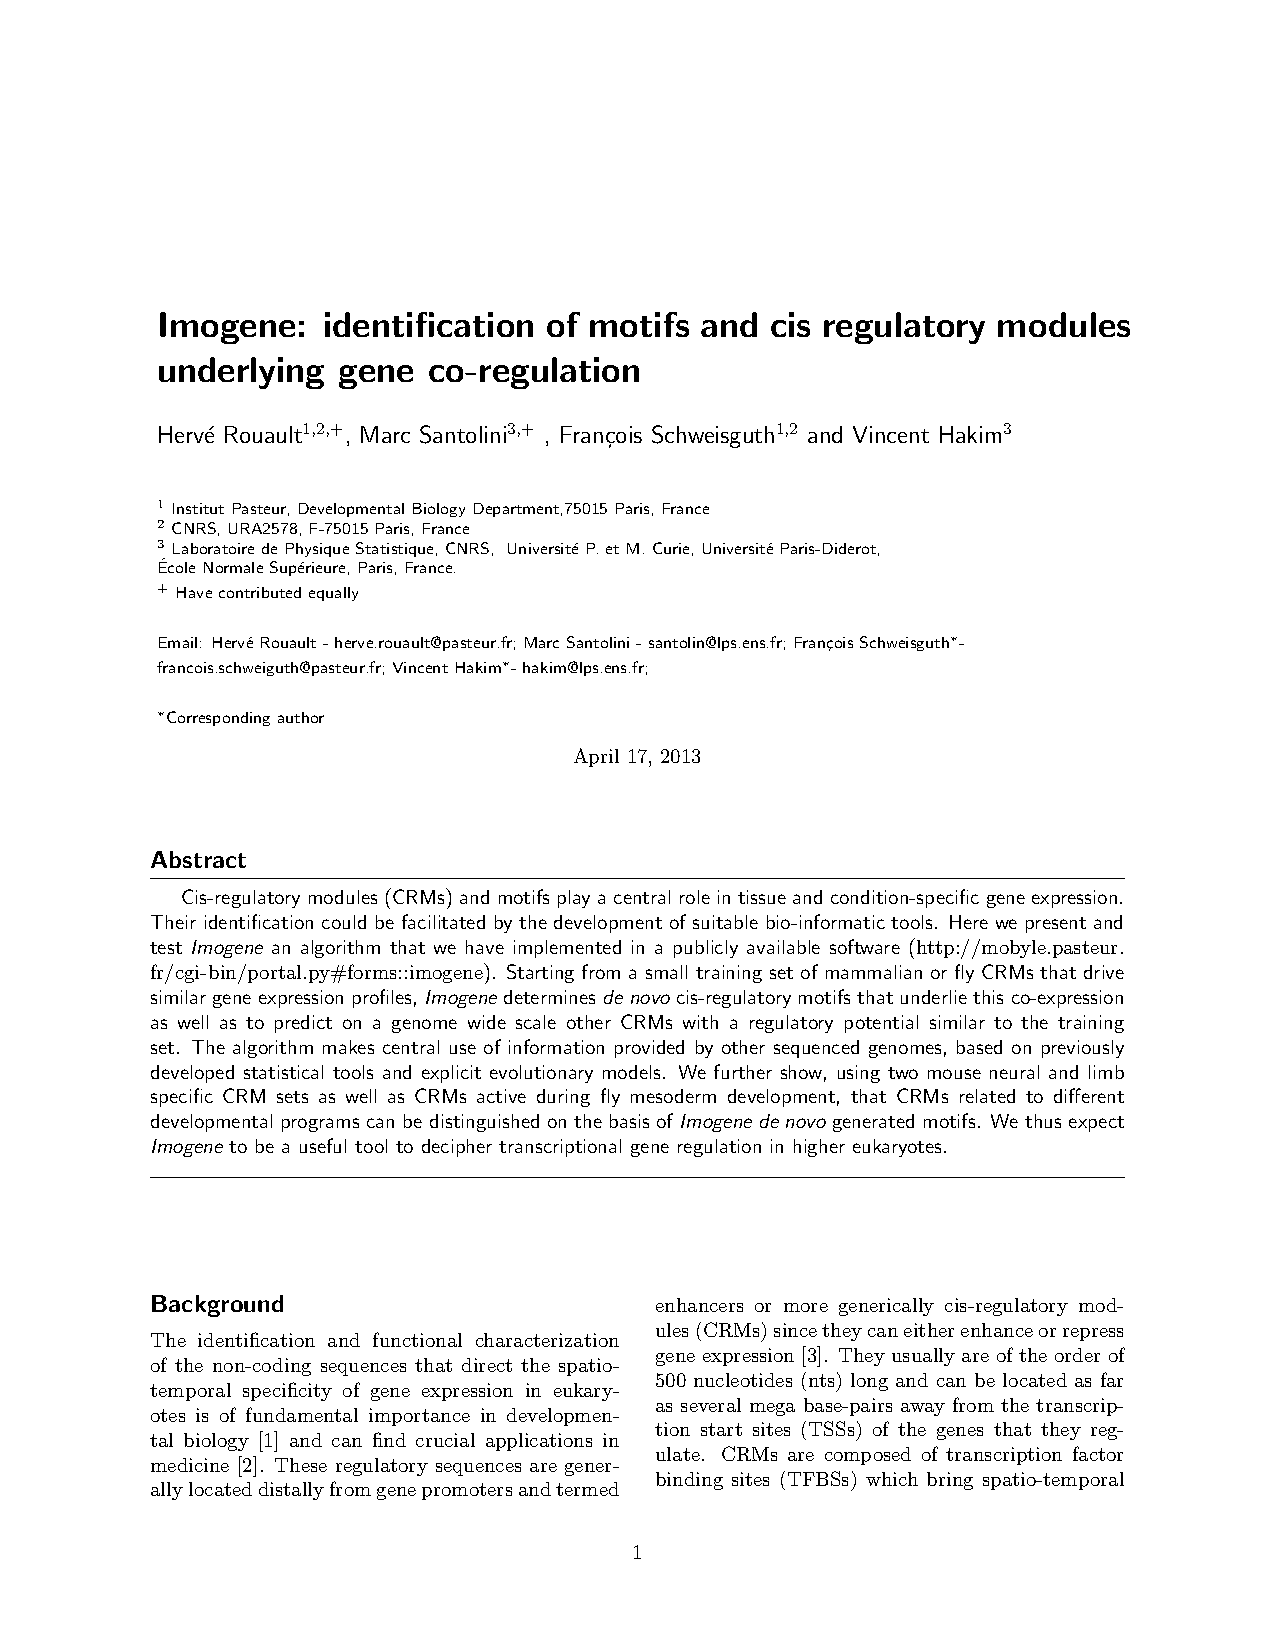
\includepdf[pages=-]{articles/imogene-genomebiol.pdf}


% section article (end)




\section{Calcul de la moyenne de la post�rieure par une m�thode MCMC} 
\label{sec:calcul_de_la_moyenne_de_la_post_rieure_par_une_m_thode_mcmc}

Nous avons voulu savoir si l'approximation r�alis�e par Imogene lors du calcul
du maximum de l'estimateur de la post�rieure modifi�e donnait un r�sultat
effectivement proche du calcul de la moyenne de l'estimateur de la post�rieure
non modifi�e $\mathcal{P}(w_i|\{\mathcal{A}\})$, o� $w_i$ est le vecteur de
poids de la PWM � la position $i$ et $\{\mathcal{A}\}$ est l'ensemble des
alignements de nucl�otides observ�s � cette position dans les sites de
fixation. N�anmoins, l'estimation de la moyenne de cette distribution est
difficile, puisque nous n'avons pas de moyen simple de l'�chantillonner. Afin
de contourner ce probl�me, nous avons eu recours � une m�thode de Monte-Carlo
par cha�nes de Markov ou MCMC bas�e sur l'algorithme de
Metropolis-Hastings~\cite{krauth2006statistical}. 


\subsection{Principe de l'algorithme de Metropolis-Hastings}
\label{sub:principe_de_l_algorithme_de_metropolis_hastings}

L'algorithme de Metropolis-Hastings
\cite{metropolis1953equation,hastings1970monte} permet d'�chantillonner la
distribution de la distribution post�rieure en utilisant le parcours d'une
cha�ne de Markov ayant cette distribution pour loi stationnaire. Une tel
processus de Markov est d�fini par des probabilit�s de transition $P(w \to w')$
entre deux �tats $w$ et $w'$. Il converge vers une distribution stationnaire
$\pi(w)$ unique sous deux conditions : (1) les transitions sont r�versibles et
le processus satisfait le bilan d�taill� $\pi(w)P(w\to w') = \pi(w')P(w'\to
w)$, (2) le processus est ergodique, \cad que tout �tat est accessible et qu'il
n'y a pas de cycles.  L'algorithme de Metropolis-Hastings repose sur la
construction d'une cha�ne de Markov ayant ces propri�t�s et dont la
distribution d'�quilibre $\pi(w)$ est la probabilit� que l'on cherche
� �chantillonner $P(w)$. Pour cela, on part de l'�quation du bilan d�taill�,
que l'on peut �crire 

\begin{equation}
    \label{eq:bilan-detaille}
    \frac{P(w \to w')}{P(w' \to w)} = \frac{P(w')}{P(w)}
\end{equation}

La transition $P(w \to w')$ est ensuite d�compos�e en deux sous-�tapes, la
proposition (\textit{proposal}) et l'acceptation (\textit{acceptance}) : 

\begin{equation}
    P(w \to w') = \underbrace{g(w \to w')}_{\text{proposition}} \cdot \underbrace{A(w\to w')}_{\text{acceptation}}
\end{equation}

En ins�rant dans l'�q. \ref{eq:bilan-detaille} on obtient

\begin{equation}
    \frac{A(w \to w')}{A(w' \to w)} = \frac{P(w')}{g(w \to w')} \frac{g(w' \to w)}{P(w)}
\end{equation}

Plusieurs choix de la fonction d'acceptation sont possibles pour satisfaire
cette �quation \cite{hastings1970monte}. Un choix courant, dit choix de
Metropolis,  est :

\begin{equation}
    \label{eq:acceptance}
    A(w \to w') = \min\left(1, \frac{P(w')}{g(w \to w')} \frac{g(w' \to w)}{P(w)}\right)
\end{equation}

Un aspect tr�s pratique de cette quantit� est qu'elle est invariante sous
multiplication de la distribution $P(w)$ par un facteur non nul. Autrement dit,
la distribution n'a pas besoin d'�tre normalis�e. Dans un cadre bay�sien, cela
veut dire que l'on peut remplacer la post�rieure par le produit de la
vraisemblance et du \textit{prior}.\\

La m�thode de Metropolis-Hastings se
r�sume donc ainsi :

\begin{enumerate}
\item Initialiser $w$ � une valeur prise au hasard.
\item Choisir un nouvel �tat $w'$ tir� selon $g(w \to w')$
\item Accepter l'�tat avec une probabilit� donn�e par $A(w \to w')$. Si le nouvel �tat n'est pas accept�, alors $w'=w$.
\item It�rer jusqu'� convergence
\end{enumerate}

Au final, $w$ �tant tir� selon la distribution $P(w)$, sa moyenne est
directement accessible en sommant les poids $w_i(t)$ obtenus au cours des $N$
it�rations r�alis�es :

\begin{equation}
    \langle w \rangle \simeq \frac{1}{N} \sum_{t=1}^N w_i(t)
\end{equation}

Quant au crit�re de convergence, une possibilit� est d'utiliser le Th�or�me
Central Limite (TCL). Celui-ci stipule que la moyenne de $n$ variables
al�atoires ind�pendantes et identiquement distribu�es selon une loi de moyenne
$\mu$ et d'�cart-type $\sigma$ de valeurs finies suit, pour $n$ grand, une loi
normale de moyenne $\mu$ et d'�cart-type $\sigma/\sqrt{n}$. Dans notre cas, les
�chantillons successifs $w_i$ ne sont pas ind�pendants � cause du fait qu'on
les tire selon la loi $g(w\to w')$. Il faut donc calculer le temps de
d�corr�lation $T$ pour lequel $\langle w_i(t) w_i(t+T) \rangle \simeq 0$, puis
utiliser les �chantillons $w_i(t)$ obtenus toutes les $T$ it�rations comme
variables ind�pendantes.  L'application du TCL permet alors d'arr�ter les
it�rations lorsqu'une certaine pr�cision d�sir�e est atteinte, par exemple
lorsque $\sigma / \sqrt{n} < 1.96$, crit�re qui assure que l'on conna�t la
vraie valeur moyenne � $95\%$ de confiance.  L'�cart-type $\sigma$ �tant lui
m�me estim� � partir des �chantillons de l'algorithme, il faut aussi s'assurer
qu'il a converg�.



% subsection principe_de_l_algorithme_de_metropolis_hastings (end)

\subsection{Application au calcul de la post�rieure}
\label{sub:application_au_calcul_de_la_post_rieure}

Dans notre cas, nous souhaitons utiliser l'algorithme de Metropolis-Hastings
pour calculer la valeur moyenne du vecteur de poids $w_i$ en
position $i$ de la PWM selon la distribution post�rieure
$\mathcal{P}(w_i|\{\mathcal{A}\})$:

\begin{equation}
    \langle w_i \rangle = \int w_i \mathcal{P}(w_i|\{\mathcal{A}\}) \text{d}w  %\simeq \sum_{t=1}^N w_i(t)
\end{equation}

Il nous faut pour cela d�finir une loi de proposition $g(w_i \to w_i')$
pertinente. Dans notre cas, les poids $w_i$ doivent rester dans le simplexe de
dimension $3$ d�fini par $w_A, w_C, w_G >0$ et $w_A+w_C+w_G <1$, le poids $w_T$
�tant enti�rement d�termin� par la normalisation des probabilit�s
$w_T=1-w_A-w_C-w_G$.  La distribution naturelle poss�dant cette propri�t� est
la loi de Dirichlet $\text{Dir}(\al)$, de param�tres
$\al=\{\al_A,\al_C,\al_G,\al_T\}$ et de densit� de probabilit�

\begin{equation}
    f(w) = \frac{1}{B(\alpha)} \prod_{b\in \{A,C,G,T\}} w_{i,b}^{\al_b - 1}
\end{equation}

o� $B(\al)$ est la fonction b�ta multinomiale permettant la normalisation.
Cette distribution est la m�me que celle obtenue dans le cas d'observations
ind�pendantes (cf article). Afin d'acc�l�rer l'�chantillonnage MCMC, nous avons
cherch� � r�gler les param�tres $\al$ de mani�re � �tre au plus proche de la
distribution $\mathcal{P}(w_i|\{\mathcal{A}\})$. Dans le cas de $N$ sites
ind�pendants, celle-ci suit une loi de Dirichlet de param�tres $\al_p + N_i$,
o� $\al_p$ est le vecteur de pseudo-counts et $N_i$ le vecteur donnant les
nombres d'observations des nucl�otides � la position $i$ au sein des
diff�rentes s�quences. Dans le cas r�el, le nombre effectif d'observation est
moins grand que le nombre total de s�quences du fait du mod�le d'�volution.
Nous avons donc d�fini les param�tres de notre \textit{proposal} comme �tant

\begin{equation}
    \al_b = \al_p + N_{\text{eff}}\cdot w_i
\end{equation}

o� $N_{\text{eff}}=N_{\text{sites}}\cdot N_{\text{spe}} /2$ avec
$N_{\text{sites}}$ le nombre d'alignements observ�s et $N_{\text{spe}}$ le
nombre total d'esp�ces dans l'alignement. Grossi�rement, cela revient � dire
que le mod�le d'�volution r�duit d'un facteur $2$ le nombre de s�quences
ind�pendantes. Nous avons calcul� que le taux d'acceptation pour ce param�tre
�tait de l'ordre de $50\%$, une valeur g�n�ralement consid�r�e comme
raisonnable~\cite{krauth2006statistical}. Nous obtenons finalement l'expression
pour la \textit{proposal} :


\begin{equation}
    g(w \to w') = \frac{1}{B(\alpha)} \prod_{b\in \{A,C,G,T\}} (w_{i,b}')^{\al_{p,b} + N_{\text{eff}}\cdot w_{i,b}  - 1}
\end{equation}

Le vecteur $w_i$ est initialis� � la valeur qu'il prendrait si toutes les
s�quences orthologues �taient des observations ind�pendantes  (cf article) :

\begin{equation}
    w_i(0) = \frac{N_i + \al_b}{N_{\text{tot}} + \sum_b \al_b}
\end{equation}


Le poids $w_i(1)$ suivant est ensuite tir� selon la probabilit� de transition
$g(w_i(0) \to w_i(1))$. Les diff�rentes quantit�s de l'�quation
\ref{eq:acceptance} sont ensuite calcul�es et la transition est accept�e avec
probabilit� $A(w_i(0) \to w_i(1))$. 
\\

Reste le probl�me de la convergence. 


\bfig
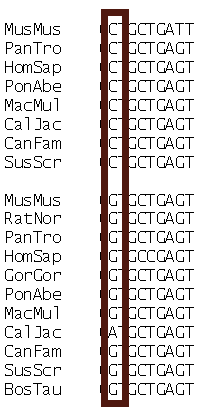
\includegraphics[width=0.8\textwidth]{figures/MCMC/TFBS.pdf}
\captionbf{Sites utilis�s pour le MCMC}{

Main caption

}
\label{fig:MCMC/TFBS}
\efig

% subsection application_au_calcul_de_la_post_rieure (end)

% section calcul_de_la_moyenne_de_la_post_rieure_par_une_m_thode_mcmc (end)

\newpage

%%%%%%%%%%%%%%%%%%%%%%%%%%%%%%%%%%%%%%%%%%%%%%%%%%%%%%%%%%%%%%%%%%%%%%%%%%%%%%%%%%%%%%%%%%%
\chapter{\ChTrichomes}
\ifthenelse{\FaitMinitocs > 0}{\adjustmtc \minitoc}{Minitoc}
\newpage
\section*{Introduction du chapitre \thechapter}

Nous pr�sentons maintenant une application de Imogene au cas de la
diff�renciation des trichomes (poils) chez la Drosophile, r�alis�e en
collaboration avec l'�quipe de Serge Plaza � l'Universit� Paul Sabatier.
Plusieurs motifs ont �t� g�n�r�s � partir de $14$ CRMs connus pour r�guler le
processus de diff�renciation des trichomes. Parmi les motifs g�n�r�s, deux
d'entre eux ont montr� une meilleure capacit� � distinguer les CRMs positifs de
l'ensemble d'apprentissage de CRMs n�gatifs. Le crit�re de distinction est bas�
sur l'optimisation de Pareto, caract�risant la satisfaction de plusieurs
contraintes � la fois. Dans notre cas, les contraintes sont de maximiser le
nombre de CRMs positifs trouv�s par les motifs (maximisation de la sensibilit�)
tout en minimisant le nombre de faux positifs (maximisation de la sp�cificit�).
Ces crit�res d�finissent une fronti�re de Pareto de motifs optimum. En variant
les diff�rents param�tres de Imogene, nous avons trouv� deux motifs sur la
fronti�re de Pareto. Parmi les deux motifs, l'un d'eux (\og svbf7 \fg)
correspond au r�gulateur ma�tre du processus de diff�renciation des trichomes,
et l'autre (\og blue motif\fg) est un motif nouveau. L'importance des deux
motifs pour la r�gulation est montr�e par mutagen�se. Par ailleurs, ces motifs
permettent de distinguer des \chipseq pour \textit{svb} li�s � une r�gulation
(dont le g�ne le plus proche subit une perte d'expression lors du KO de
\textit{svb}) des \chipseq ne l'�tant pas. Ce travail montre donc un exemple de
la possibilit� d'utiliser Imogene sur sun un petit ensemble (ici $14$ CRMs) de
donn�es biologiques fonctionnelles pour d�tecter des motifs nouveaux et
fonctionnels.

\newpage

\section{Concept d'optimum de Pareto} 
\label{sec:concept_d_optimum_de_pareto}

Dans l'article qui suit, nous utilisons le principe d'optimum de Pareto, li�
� la satisfaction simultan�e de plusieurs contraintes. Le probl�me est le
suivant. �tant donn�s $14$ CRMs positifs li�s � une m�me r�gulation de la
diff�renciation des trichomes chez l'embryon de Drosophile, et $25$ CRMs
n�gatifs ne conduisant aucune expression au stade de d�veloppement consid�r�,
quels motifs permettent le mieux de distinguer les deux classes? Le probl�me
est similaire � celui de \textit{pattern recognition} introduit dans l'article
pr�c�dent en section \ref{sec:article_imogene}. N�anmoins, nous avons ici
adopt� une d�marche l�g�rement diff�rente. 

Des motifs sont appris sur les CRMs positifs pour diff�rents seuils $S_g$
(variant entre $7$ et $13$ bits). Ces motifs sont ensuite utilis�s pour pr�dire
les CRMs positifs parmi les CRMs initiaux. Un CRM est d�clar� comme positif
s'il contient au moins  $n$ sites conserv�s ($n=1$, $2$, ou $3$) au-dessus d'un
seuil $S_s$ (variant entre $7$ et $13$ bits). Pour des param�tres $S_g$, $n$ et
$S_s$ donn�s, un motif d�tectera un nombre FP de Faux Positifs (les CRMs
n�gatifs qui sont pr�dits positifs) et omettra un nombre FN de Faux N�gatifs
(les CRMs positifs qui ne sont pas pr�dits comme tels). L'optimisation de
Pareto consiste � trouver les param�tres $S_g$, $n$ et $S_s$ qui minimisent
� la fois FP et FN. Il est possible de minimiser diff�rentes fonctions de co�t
pour FP et FN, attribuant des poids plus ou moins importants � l'une ou l'autre
des contraintes. Dans notre cas, nous avons d�fini l'optimum de Pareto comme
minimisant la fonction $|\text{FN}+\text{FP}|$.  La droite
$|\text{FN}+\text{FP}|=cte$ contenant les meilleurs optima de Pareto pour les
diff�rents motifs est la fronti�re de Pareto. 

Dans notre cas, deux des motifs g�n�r�s sont sur la fronti�re de Pareto : le
motif svbF7 et le motif bleu (fig.~\ref{fig:plaza/pareto/plot_pareto}), pour
$S_g=10$ bits, $n=1$, $S_s=8.5$ bits. Ce sont par ailleurs les $2$ premiers
motifs g�n�r�s � ce seuil. Les $3$ motifs suivants sont montr�s en gris. Le
motif svbF7 correspond au TF \textit{svb} (\textit{Shavenbaby}), r�gulateur
ma�tre de la diff�renciation des trichomes. Le motif OvoQ6 correspond � la PWM
de Transfac pour \textit{svb}, et n'apporte pas une aussi bonne classification
que svbF7. Le motif bleu, quant � lui, n'est pas connu. Nous montrons aussi le
motif jaune, introduit dans l'article, qui n'est pas pr�dit par Imogene mais
correspond � un motif de r�gulation ultra-conserv� dans les de diff�rentes
esp�ces de drosophiles~\cite{Elemento2005fk}, et poss�dant un r�le fonctionnel
investigu� par mutagen�se.


\bfig
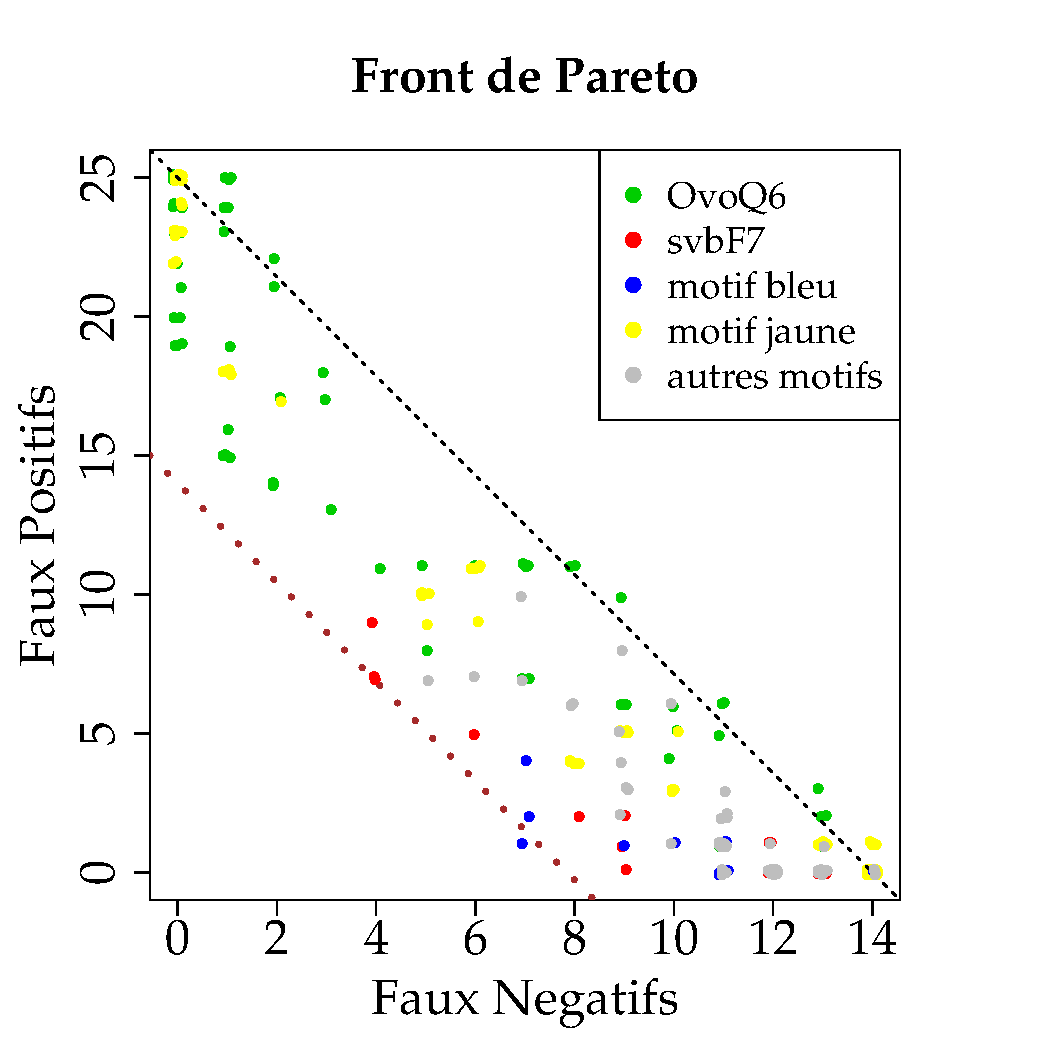
\includegraphics[width=1\textwidth]{figures/plaza/pareto/plot_pareto.pdf}
\captionbf{Fronti�re d'efficacit� de Pareto}{

    Illustration de l'optimisation de Pareto permettant la s�lection des
    param�tres lors de la g�n�ration de motifs. Ici, nous voulons � la fois
    minimiser le nombre de Faux Positifs (FP) et le nombre de Faux n�gatifs
    (FN).  Diff�rents motifs sont successivement utilis�s pour classer les
    s�quences comme positives ou n�gatives, une s�quence �tant d�clar�e comme
    positive pour un motif si elle contient au moins $n$ sites conserv�s
    au-dessus d'un seuil $S_s$. Les diff�rents points correspondent aux
    diff�rentes performances. Un l�ger bruit a �t� ajout� aux points pour
    rendre visibles ceux qui sont superpos�s (fonction \texttt{jitter} de R,
    param�tre \texttt{factor}$=0.5$). Le motif svbF7 et le motif bleu sont tous
    deux optimaux pour des param�tres bien d�finis $S_g=10$ bits, $n=1$,
    $S_s=8.5$ bits : ils dessinent la fronti�re de Pareto $|FP+FN|=cte$ en
    pointill�s bruns.

}
\label{fig:plaza/pareto/plot_pareto}
\efig




% section concept_d_optimum_de_pareto (end)


%%%%%%%%%%%%%%%%%%%%%%%%%%%%%%%%%%%%%%%%%%%%%%%%%%%%%%%%%%%%%%%%%%%%%%%%%%%%%%%%%%%%%%%%%%%%%%%%%%%	%%%%%%%%%%%%%%%%%%%%%%%%%%%%%%%%%%%%%%%%%%%%%%%%%%%%%%%%%%%%%%%%%%%%%%%%%%%%%%%%%%%%%%%%%%%%%%%%%%%	

\newpage
\section{Article} 
\label{sec:article_plaza}

%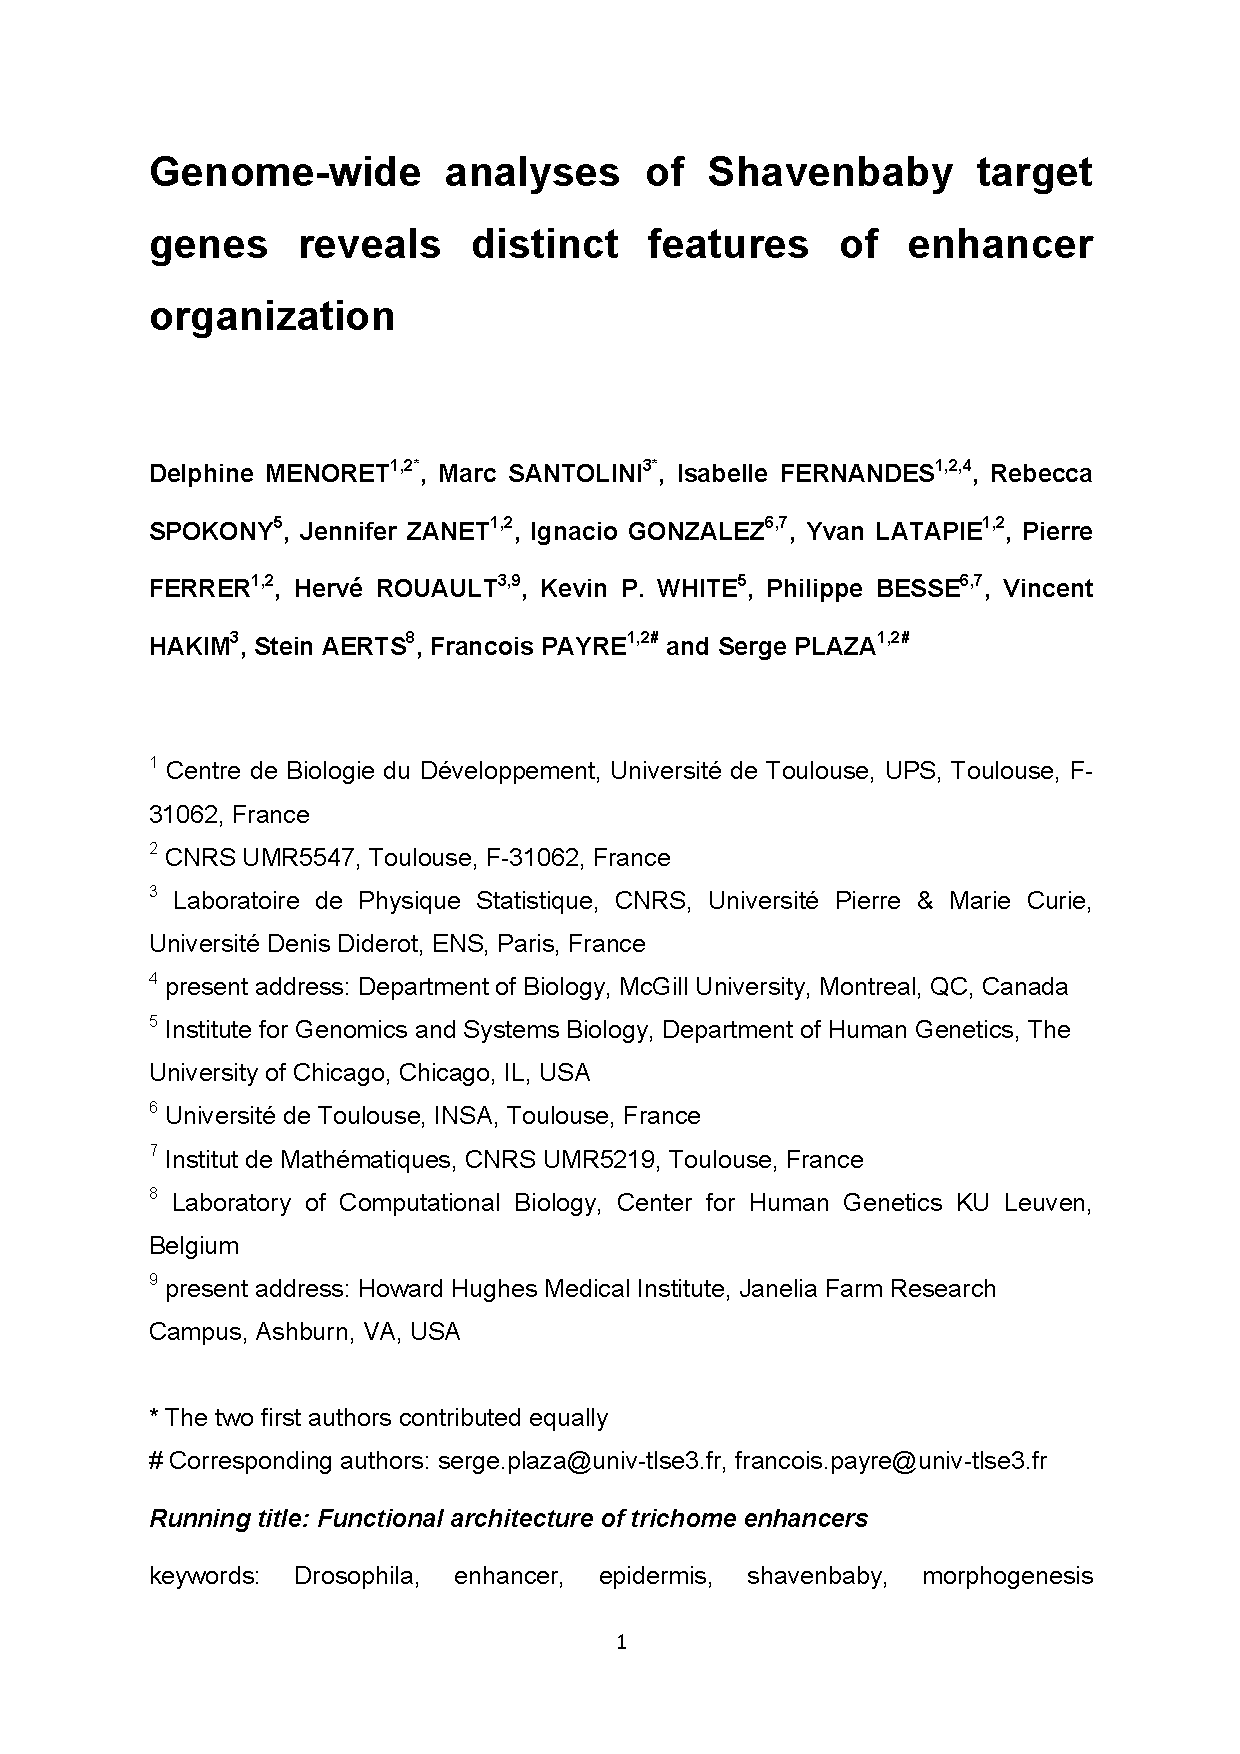
\includepdf[pages=-]{articles/trichomes-genomebiol/Menoret_et_al_GenBiol_revised.pdf}
%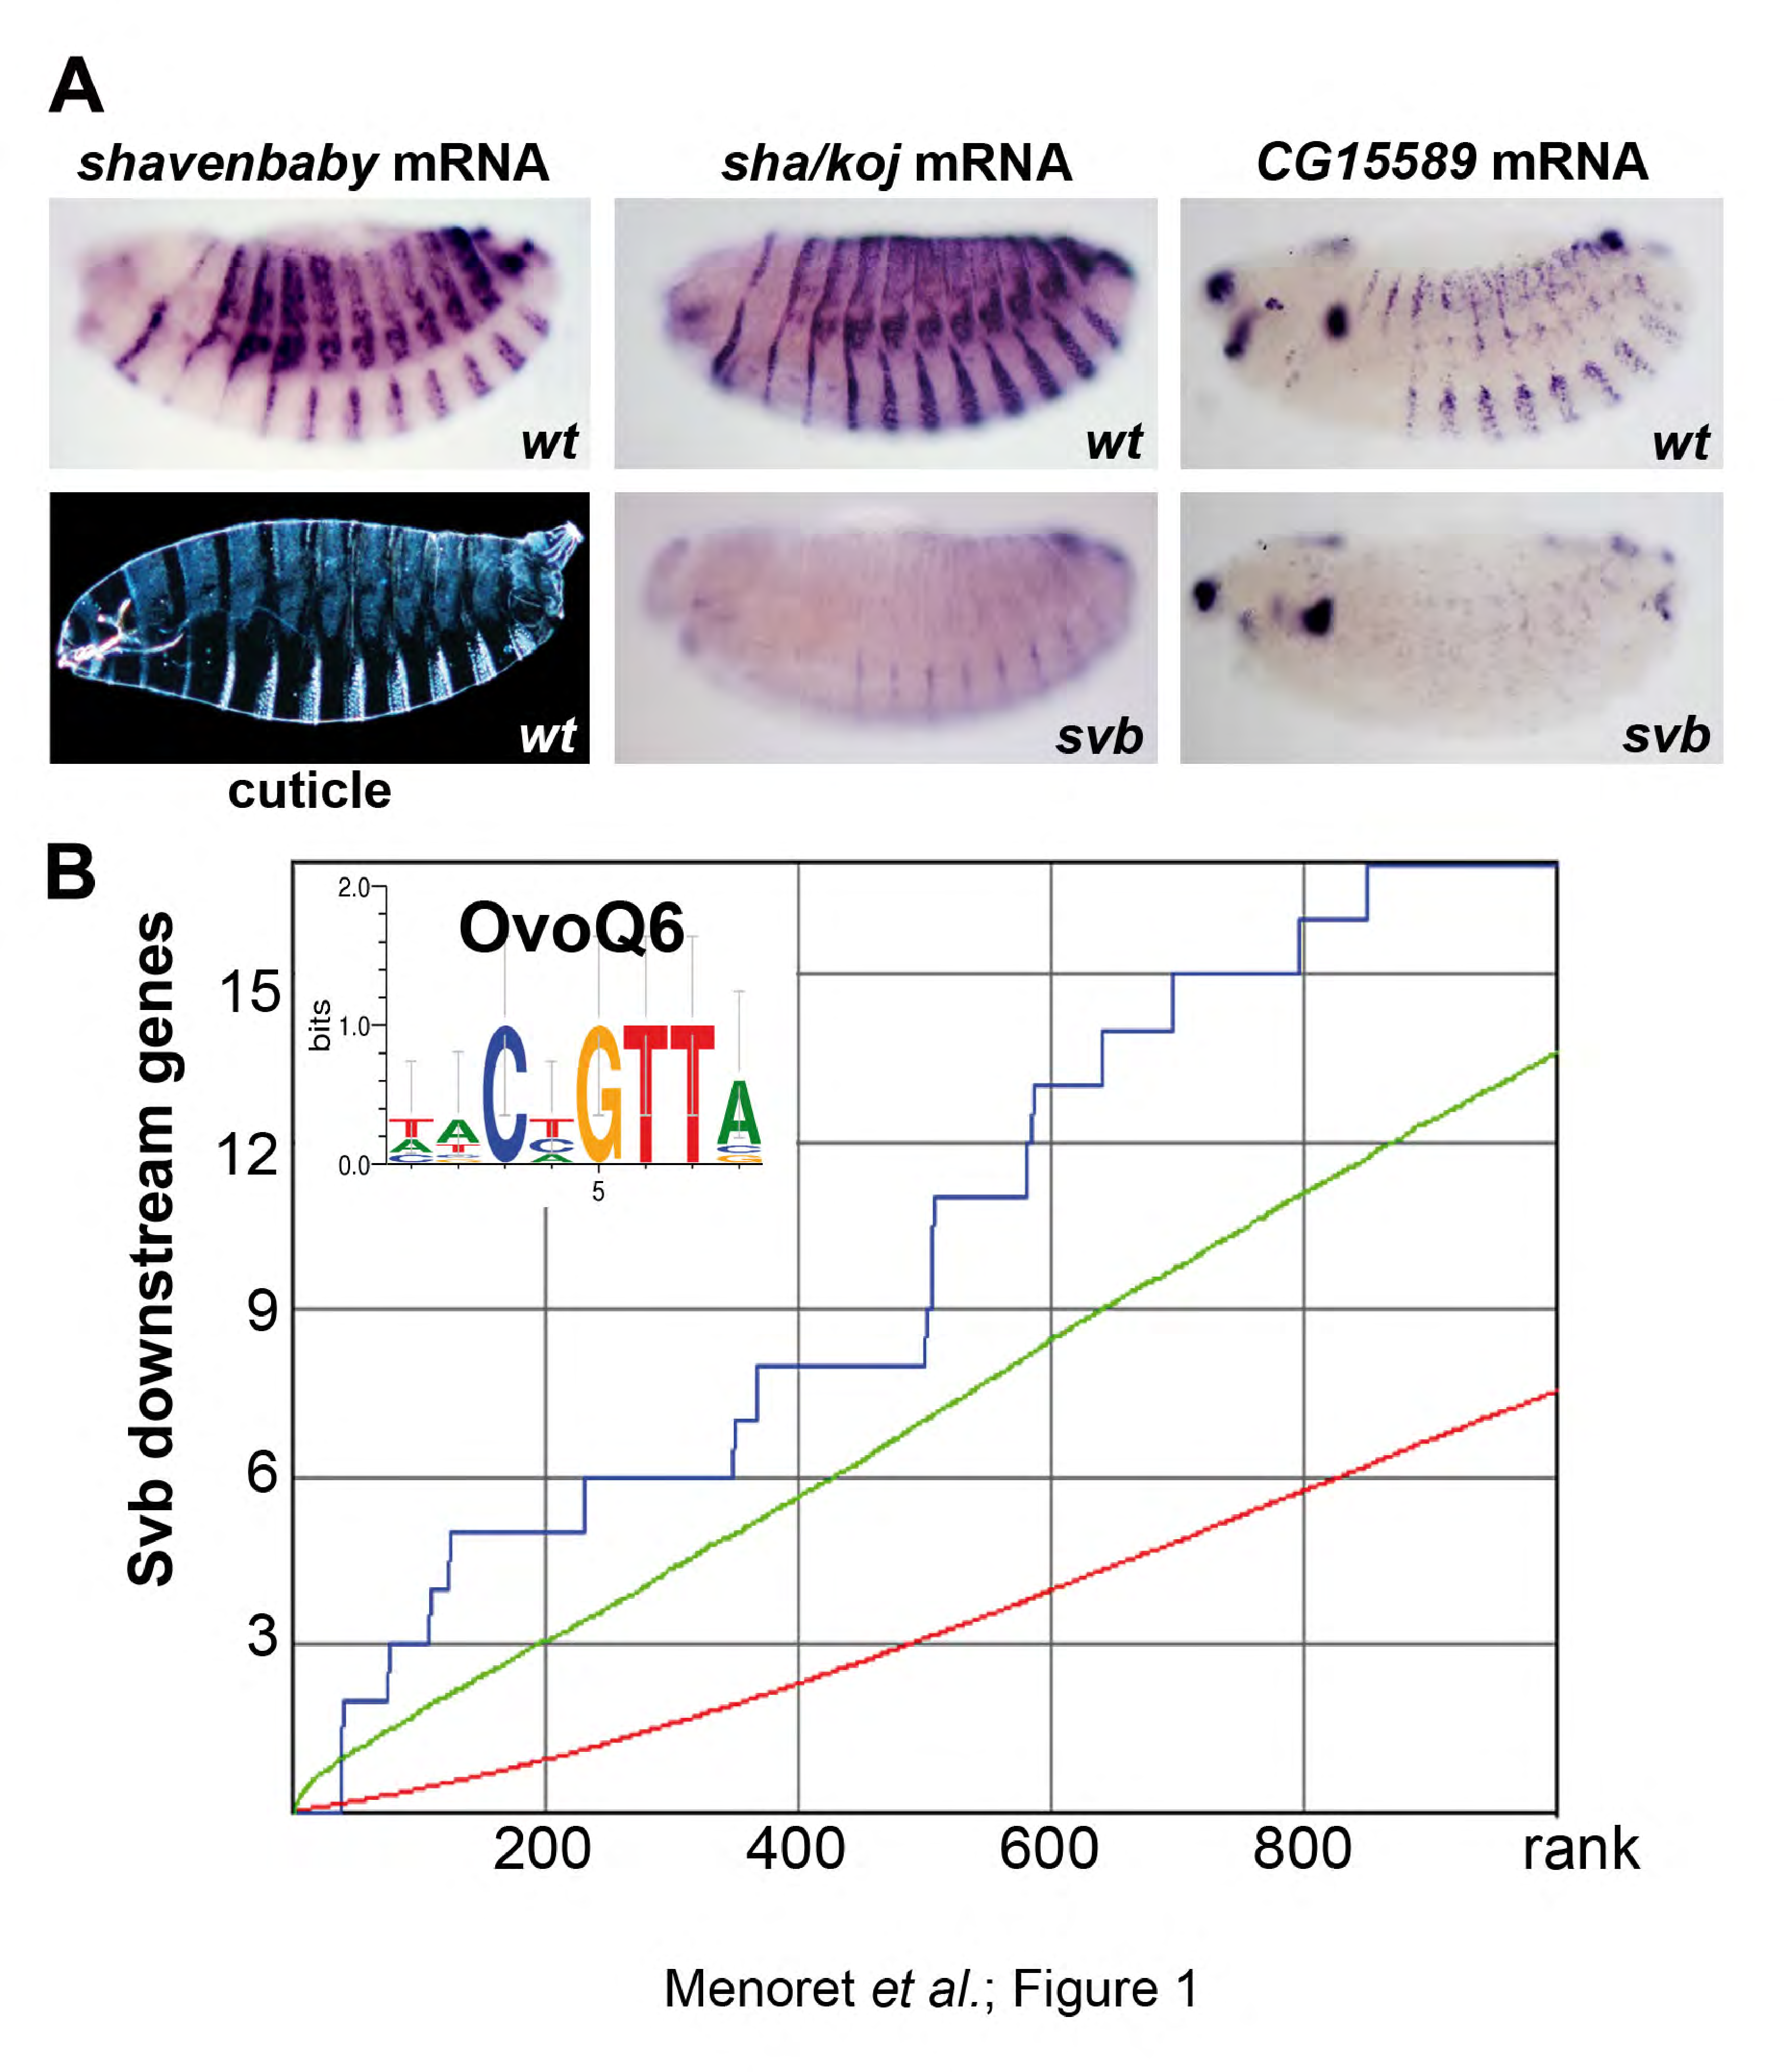
\includepdf[pages=-]{articles/trichomes-genomebiol/Figures_rev_S.pdf}
%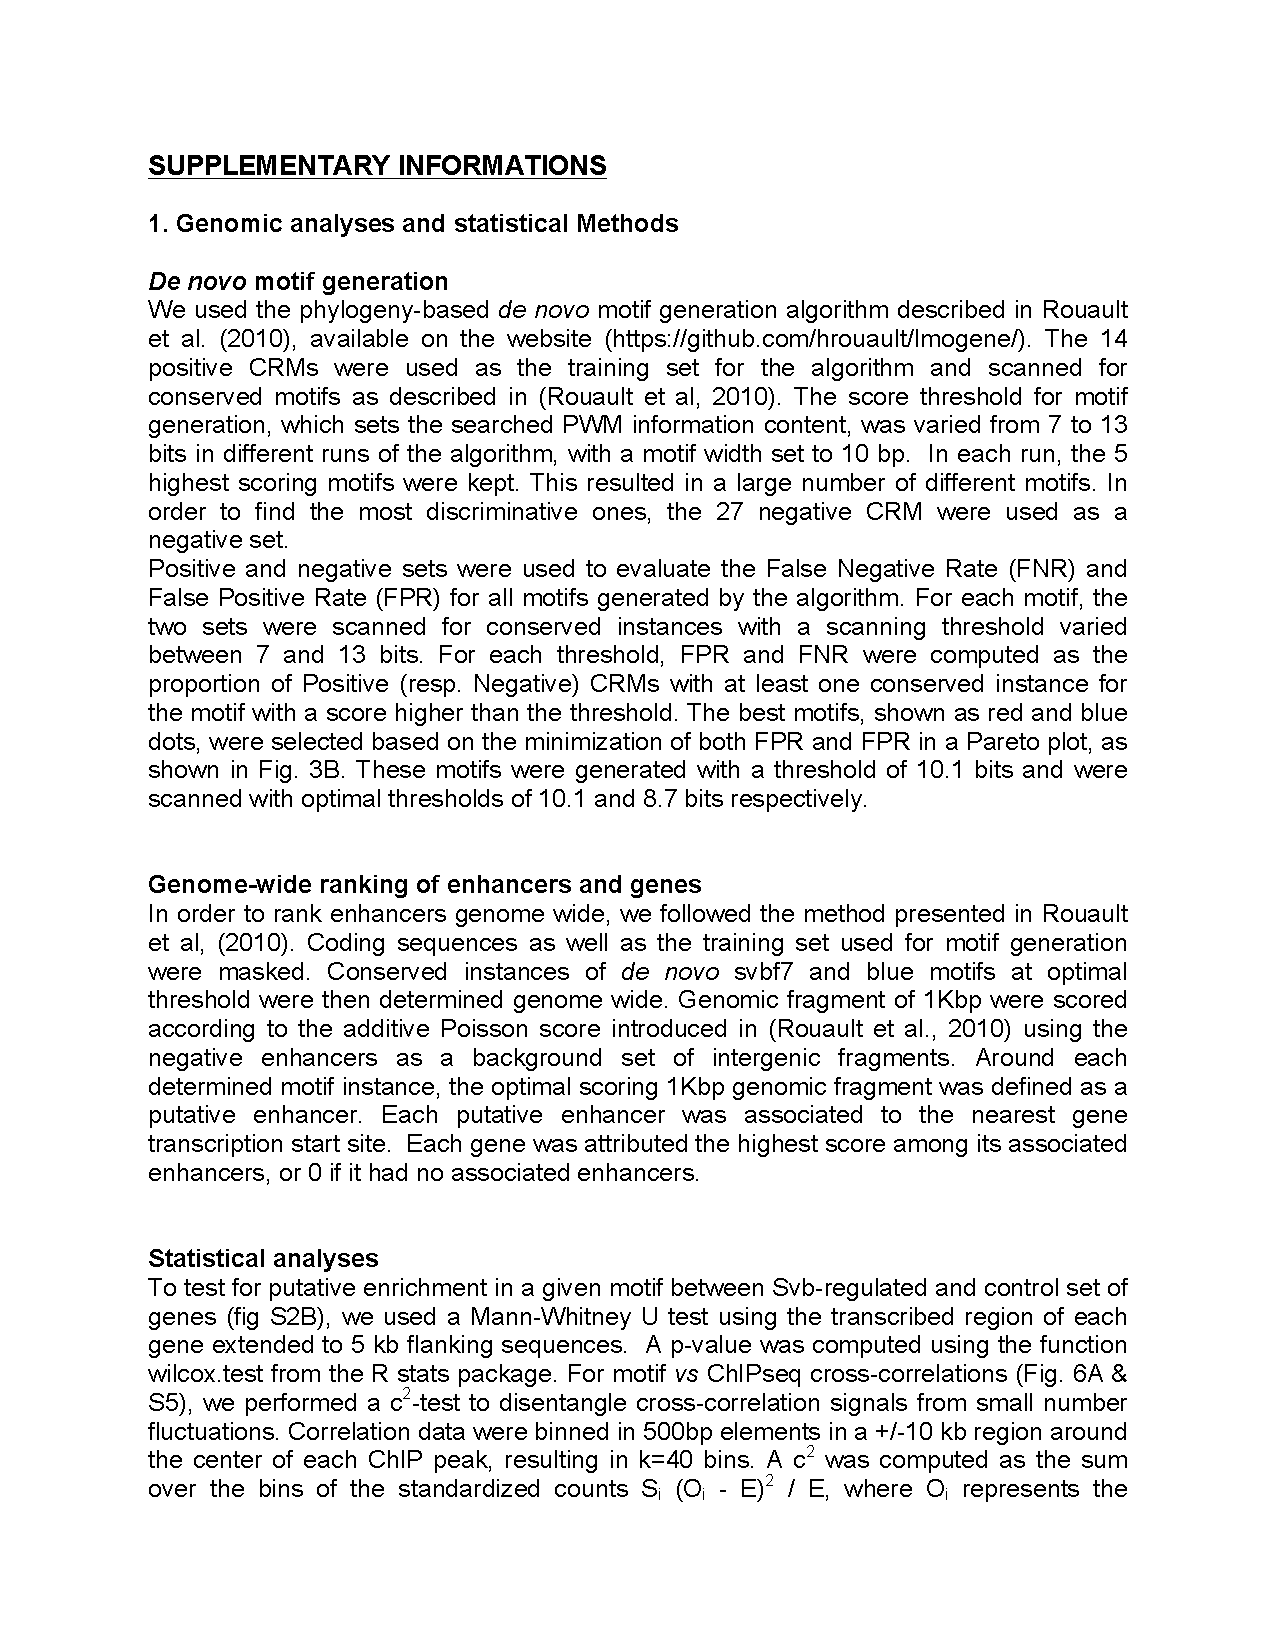
\includepdf[pages=-]{articles/trichomes-genomebiol/Menoret_SupInfos_revised.pdf}
%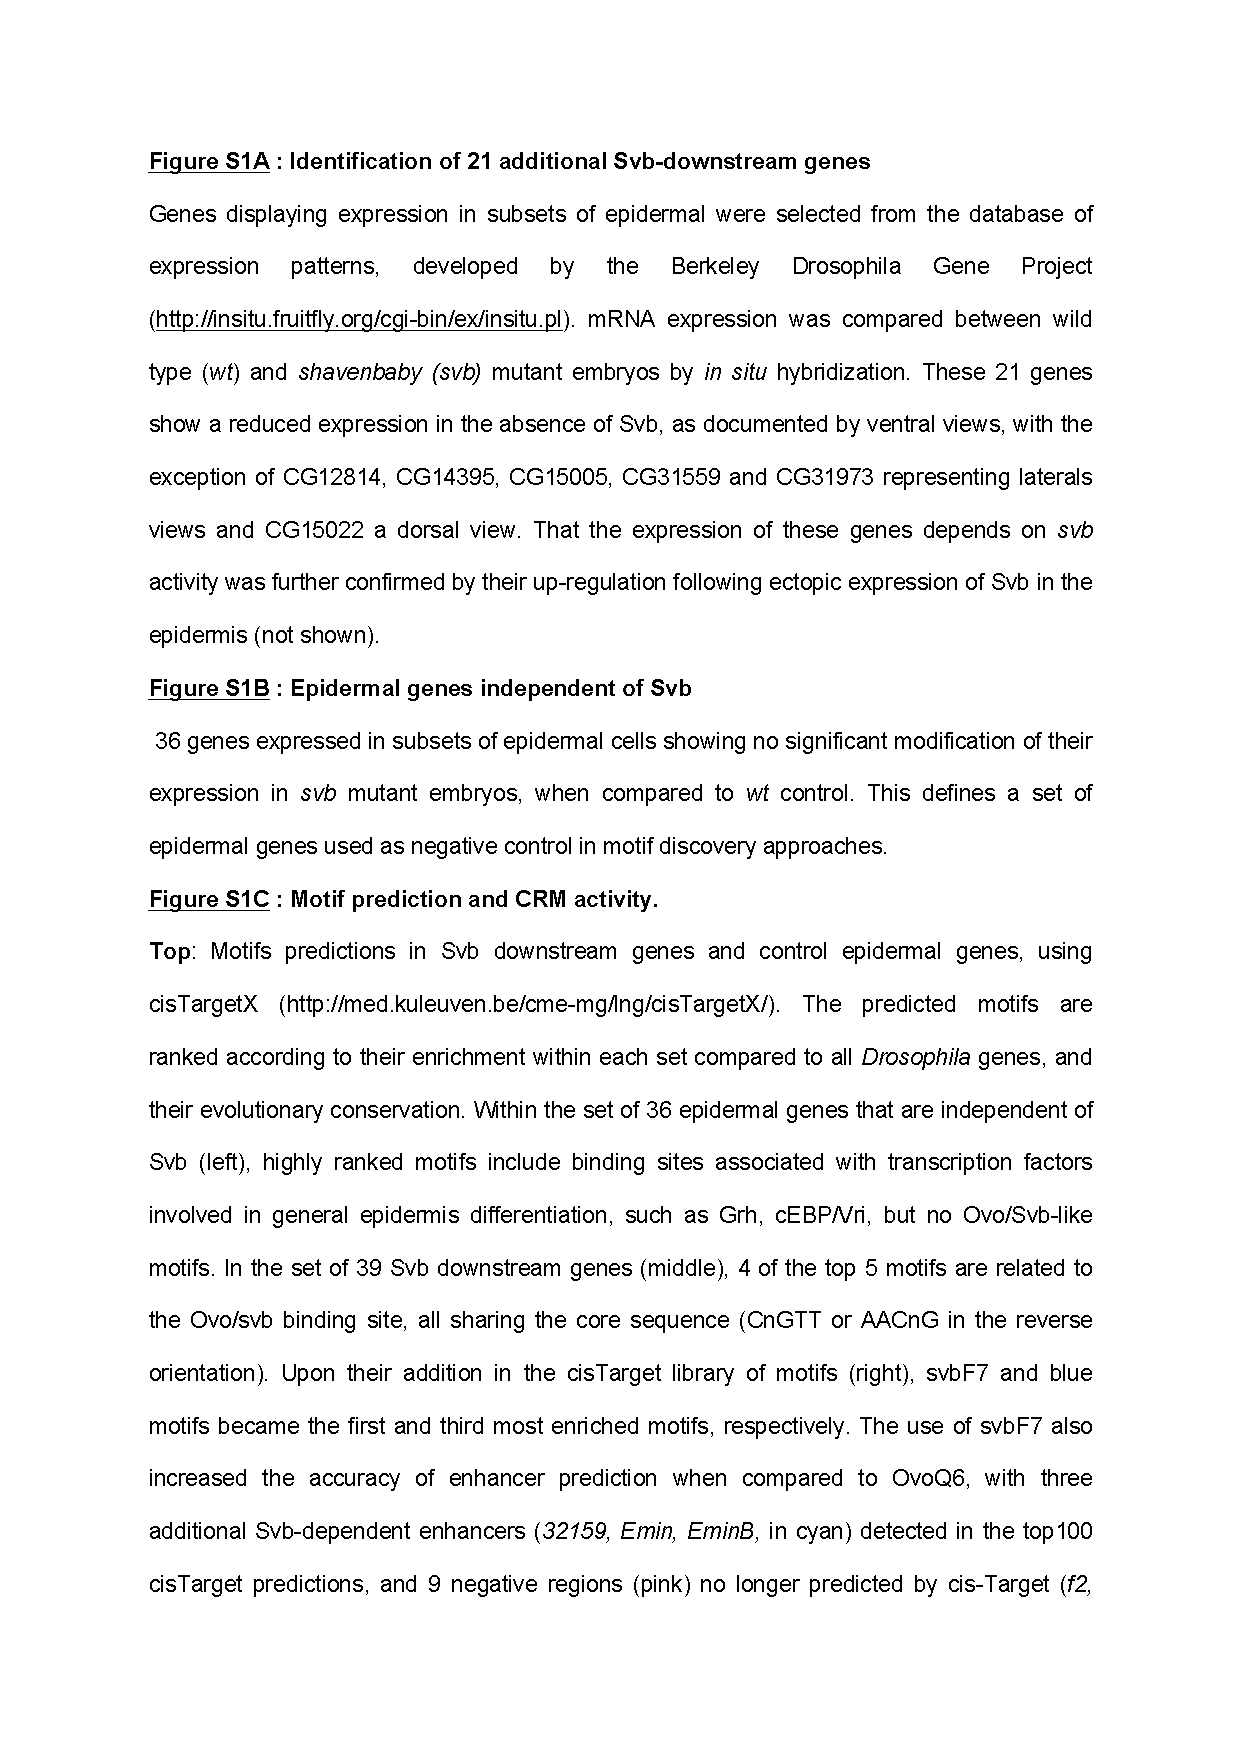
\includepdf[pages=-]{articles/trichomes-genomebiol/Menoret_et_al_FigSupLegend_revised.pdf}
%\includepdf[pages=-]{articles/trichomes-genomebiol/FigSup_rev_S.pdf}
% section article (end)
			
%%%%%%%%%%%%%%%%%%%%%%%%%%%%%%%%%%%%%%%%%%%%%%%%%%%%%%%%%%%%%%%%%%%%%%%%%%%%%%%%%%%%%%%%%%%%%%%%%%%	%%%%%%%%%%%%%%%%%%%%%%%%%%%%%%%%%%%%%%%%%%%%%%%%%%%%%%%%%%%%%%%%%%%%%%%%%%%%%%%%%%%%%%%%%%%%%%%%%%%	
\newpage	
			

\section{Conclusion et perspectives du chapitre \thechapter}

Imogene a �t� appliqu� sur un ensemble d'apprentissage compos� de $14$ CRMs
r�gulant la diff�renciation des trichomes chez l'embryon de Drosophile. Les
diff�rents param�tres (seuils de g�n�ration, de d�tection) ont �t� optimis�s
par une approche de Pareto visant � maximiser le nombre de CRMs positifs
pr�dits par les motifs tout en minimisant le nombre de CRMs n�gatifs pr�dits
parmi un ensemble de $25$ CRMs n'ayant aucune activit� au stade de
d�veloppement consid�r�. Deux motifs ont �t� trouv� par cette approche : le
motif svbF7 correspondant � \textit{svb}, le r�gulateur ma�tre de la
diff�renciation des trichomes, et un nouveau motif, le motif bleu, que nous
n'avons pas pu associer � un motif connu. 

La validit� de ces motifs a �t� montr�e par mutagen�se (figures $3$, $4$ et $5$
de l'article). Par ailleurs, ces motifs sont pr�dictifs des \chipseq de
\textit{svb} fonctionnels, \cad ceux qui sont associ�s � un g�ne dont
l'expression diminue chez les mutants \textit{svb} (figure S$5$). Les CRMs
fonctionnels poss�dent une grande vari�t� de grammaire des sites de fixation
(figures $5$ et $7$ de l'article), un r�sultat similaire � celui obtenu par
\citet{Zinzen2009p760} dans le cas de la diff�renciation de diff�rents tissus
chez l'embryon de drosophile. Plusieurs entr�es (combinaisons de TFs) m�nent
� une sortie (motif d'expression du g�ne rapporteur) similaire : cette
flexibilit� est r�miniscente du mod�le \textit{billboard} introduit en section
\ref{sub:enhanceosome_billboard}.  N�anmoins, bien qu'il soit clair que la
grammaire des sites soit diff�rente entre diff�rents CRMs, cette grammaire
semble relativement bien conserv�e au cours de l'�volution d'un CRM (figures 8,
S8A, et S8B).  Enfin, dans la plupart des cas on observe l'absence de
\textit{clustering} de motifs homotypiques sur les CRMs, bien que les motifs
soient pr�sents en plus grand nombre dans les loci des g�nes r�gul�s par
rapport � des g�nes non r�gul�s (figure S$2$). Une explication possible est que
'abondance de sites dans l'environnement du CRM permet d'augmenter localement
la concentration du TF pour faciliter son recrutement \invivo au niveau des
CRMs poss�dant des sites de forte affinit�.

Il serait � pr�sent int�ressant de caract�riser plus en avant le motif bleu
g�n�r� par l'approche \denovo. Une possibilit� serait d'utiliser la technique
de simple hybride pr�sent�e en
\ref{sub:approche_clonale_la_technique_de_simple_hybride} afin d'identifier la
prot�ine associ� au motif bleu, en utilisant comme app�t les prot�ines connues
de la drosophile et comme proie le site consensus du motif bleu.

 


\includepdf[pages=-]{articles/trichomes-plosbiol-merged.pdf}
\newpage
%%%%%%%%%%%%%%%%%%%%%%%%%%%%%%%%%%%%%%%%%%%%%%%%%%%%%%%%%%%%%%%%%%%%%%%%%%%%%%%%%%%%%%%%%%%
%\chapter{\ChMuscle}
%\label{chap:muscle}
%\ifthenelse{\FaitMinitocs > 0}{\adjustmtc \minitoc}{Minitoc}
%\newpage
%\section*{Introduction du chapitre \thechapter}

Cette derni�re partie est consacr�e � l'�tude de la diff�renciation musculaire.
Ce travail a �t� effectu� en collaboration avec l'�quipe de Pascal Maire
� l'Institut Cochin, qui m'a accueilli et m'a permis de r�aliser une partie des
exp�riences pr�sent�es, avec l'aide de Iori Sakakibara. Nous nous int�ressons
ici particuli�rement aux hom�oprot�ines Six$1$ et Six$4$ (\textit{Sine Oculis
Homeobox Homolog} $1$ et $4$, r�f�r�es dans la suite par \sixd) qui sont des
\tfs impliqu�s dans la r�gulation des stades successifs de la myogen�se. Ils
activent en effet les TFs n�cessaires � l'engagement de cellules pluripotentes
dans la voie myog�nique et � leur diff�rentiation : Pax3 (\textit{Paired Box
$3$}) ainsi que les Facteurs de R�gulation Myog�nique Myf5 (\textit{Myogenic
Factor $5$}), Mrf4 (\textit{Muscle-Specific Regulatory Factor $4$}, aussi
appel� Myf$6$), Myod (\textit{Myogenic Differentiation}) et Myog
(\textit{Myogenin}). Cette r�gulation passe par la fixation des prot�ines Six
sur un site \mef d'environ $10$bp. 

Nous nous sommes d'abord int�ress� aux cibles transcriptionnelles de \sixd
� l'�chelle du g�nome, ainsi qu'� leurs cor�gulateurs. Pour cela, nous avons
d'abord r�alis� un mod�le PWM des sites \mef, que nous avons utilis� pour la
pr�diction de sites. Nous avons par ailleurs r�cup�r� de nombreuses donn�es
relatives � la diff�renciation musculaire : \chipseq de TFs et des marques
�pig�n�tiques des histones, donn�es d'expression de type RNAseq, sites de
fixation conserv�s que nous avons obtenus par analyse bioinformatique, etc. Ces
donn�es ont �t� regroup�es sur le visualiseur de UCSC, permettant d'envisager
facilement le contexte de r�gulation de certains g�nes d'int�r�t. Nous
pr�sentons plusieurs validations de pr�dictions obtenues par analyse
bioinformatique avec ces donn�es.

Par ailleurs, nous nous sommes int�ress� � l'action concert�e ou
\textit{synergie} entre \sixd et le TF ma�tre MyoD au cours de la
diff�renciation musculaire. Nous avons trouv� un certain nombre de CRMs fix�s
par MyoD et poss�dant un site \mef conserv� chez les mammif�res, et dont le
g�ne le plus proche n'est activ� qu'en pr�sence de MyoD et de \sixd. Parmi les
g�nes en question figurent \myog, TF requis pour la diff�renciation terminale,
et des g�nes structuraux comme \textit{Tnnc1} (\textit{Troponin C Type $1$}) ou
\textit{Ttn} (\textit{Titin}). Nous avons test� l'activit� des CRMs pr�dits et
en avons trouv� $70\%$ qui r�capitulent l'expression du g�ne le plus proche
lorsqu'ils sont test�s par transfection avec un rapporteur Lucif�rase. Nous
avons par ailleurs utilis� Imogene pour pr�dire des cor�gulateurs et avons
test� l'importance des sites par mutagen�se.

%%%%%%%%%%%%%%%%%%%%%%%%%%%%%%%%%%%%%%%%%%%%%%%%%%%%%%%%%%%%%%%%%%%%%%%%%%%%%%%%%%%%%%%%%%%%%%%%%%%	%%%%%%%%%%%%%%%%%%%%%%%%%%%%%%%%%%%%%%%%%%%%%%%%%%%%%%%%%%%%%%%%%%%%%%%%%%%%%%%%%%%%%%%%%%%%%%%%%%%	
\newpage

\section{Introduction � la myogen�se squelettique} 
\label{sec:introduction_la_myogen_se}

\subsection{Les diff�rentes �tapes de la myogen�se}
\label{sub:les_diff_rentes_tapes}

La myogen�se correspond � la formation des tissus musculaires, ceux-ci �tant
regroup�s en trois types majeurs : les muscles cardiaques, les muscle lisses et
les muscles squelettiques. C'est la formation de ces derniers qui nous
int�resse ici. Les muscles squelettiques sont compos�s de fibres musculaires polynucl�es
provenant de la fusion de prog�niteurs musculaires appel�s myoblastes. Ils sont
sous le contr�le du syst�me nerveux central, et composent l'un des organe
majeur des vert�br�s, concentrant $\sim40\%$  du poids corporel. La
myogen�se squelettique d�bute relativement t�t au cours de l'embryogen�se : � $8.5$
jours\footnote{La mi-journ�e correspondant au fait que la f�condation a lieu la
nuit.} apr�s f�condation (ou E$8.5$ pour \textit{Embryonic day} $8.5$) chez
l'embryon de souris sur un total de $18$ jours embryonnaires. Elle a lieu au
niveau des somites, structures p�riodiques situ�es au niveau des futures
vert�bres (fig.~\ref{fig:buckingham-myogenesis}a). Les �tapes de fusion des
myoblastes et de maturation des fibres s'�talent ensuite sur toute
l'embryogen�se (fig.~\ref{fig:buckingham-myogenesis}b), ainsi que dans le
muscle adulte lors de la r�g�n�ration musculaire \cite{Parker2003p761}.

\bfigp
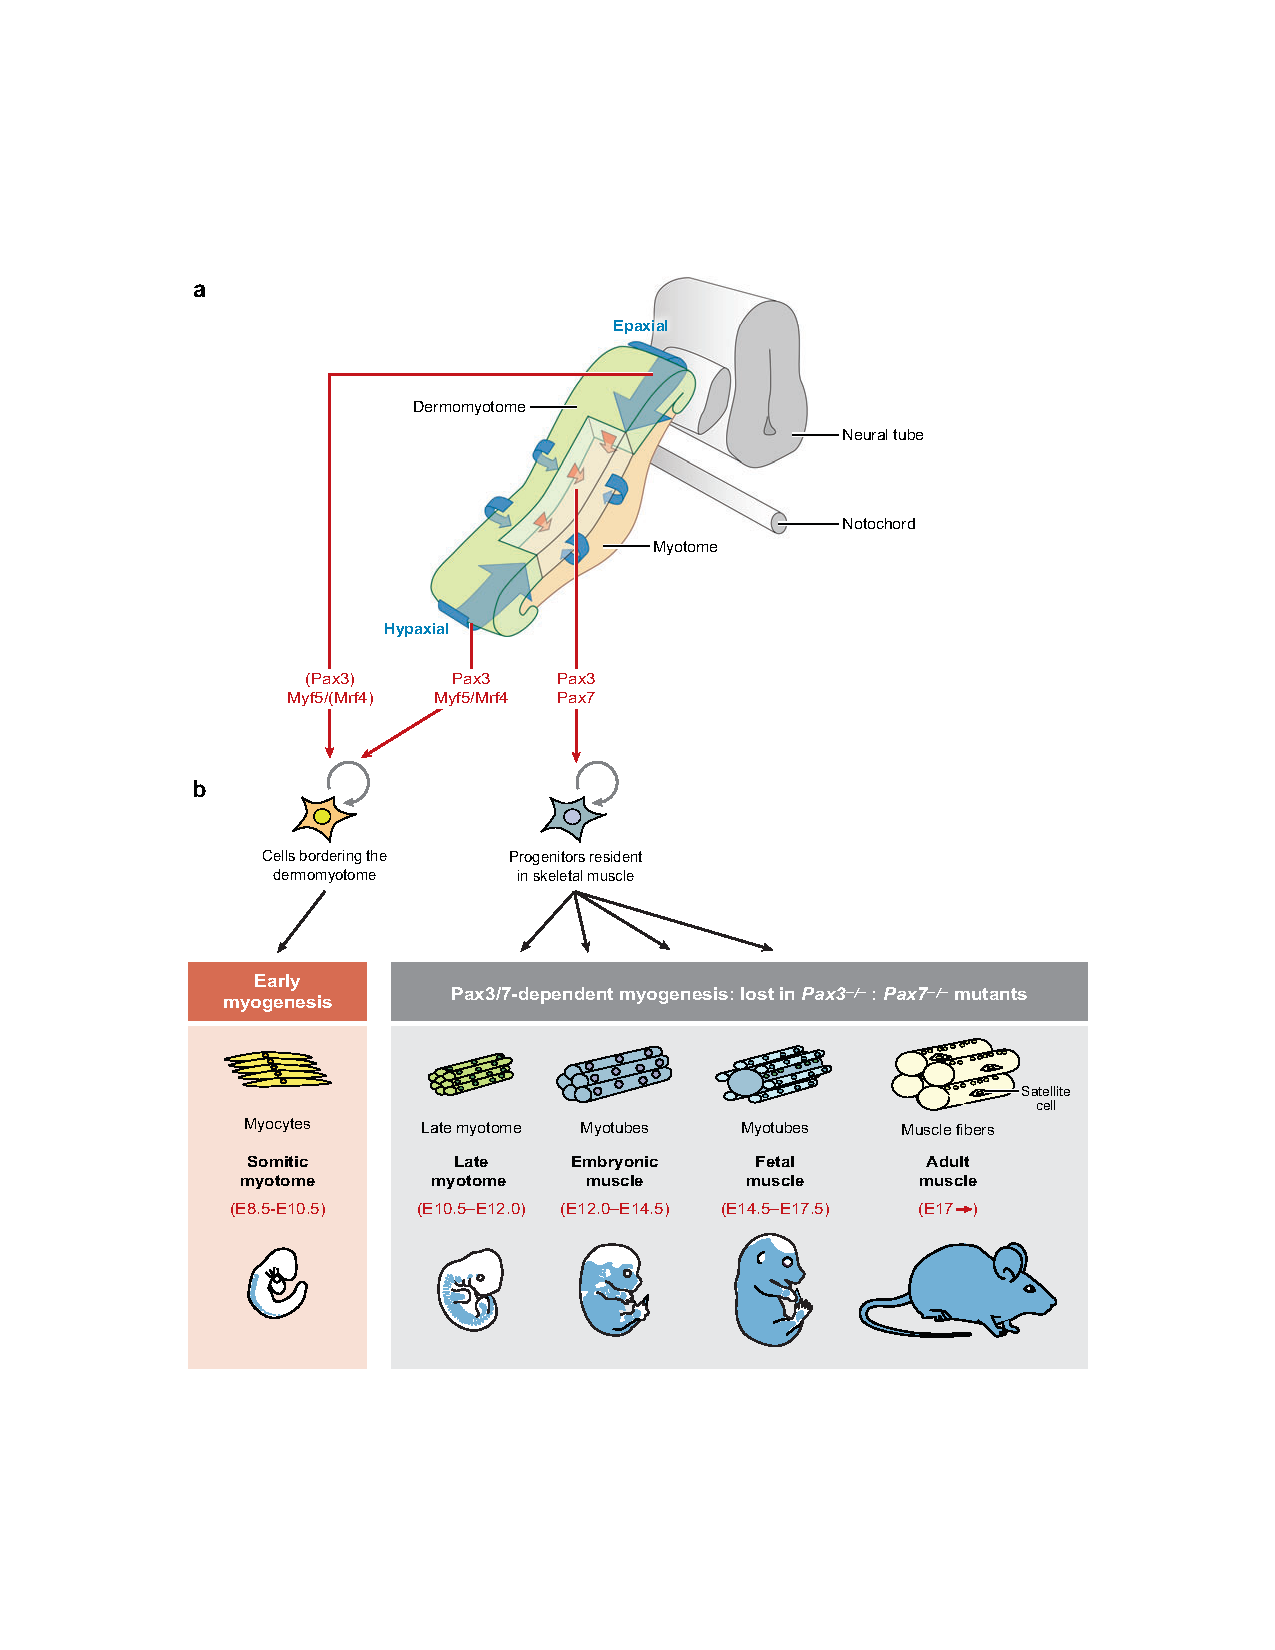
\includegraphics[width=.9\textwidth]{figures/buckingham-myogenesis.pdf}
\captionbf{Formation du muscle squelettique chez l'embryon de souris}{

    Figure tir�e de \citet{Buckingham2007p776} illustrant les diff�rentes
    �tapes de la myogen�se. (a) Le dermomyotome �pith�lial d'un somite (vert)
    ainsi que le muscle squelettique du myotome (beige) sont d'abord form�s par
    la d�lamination des cellules provenant des extr�mit�s du dermomyotome
    (fl�ches bleues) : c'est la premi�re vague de la myogen�se. Ensuite, lors
    d'une deuxi�me vague, le dermomyotome central perd sa structure �pith�liale
    et des cellules musculaires prog�nitrices s'int�grent au myotome
    (fl�ches rouges). Les TFs pr�curseurs de ces �v�nements sont indiqu�s en
    rouge. (b) Sch�ma montrant les �tapes de diff�renciation des prog�niteurs
    musculaires, ainsi que les temps de d�veloppement associ�s (E : jour
    embryonnaire).

}
\label{fig:buckingham-myogenesis}
\efigp


% subsection les_diff_rentes_tapes (end)

\subsection{Les Facteurs de R�gulation Myog�nique et leurs cofacteurs}
\label{sub:la_r_gulation_g_n_tique_les_facteurs_de_r_gulation_myog_nique_ou_mrfs}

%\bfig
%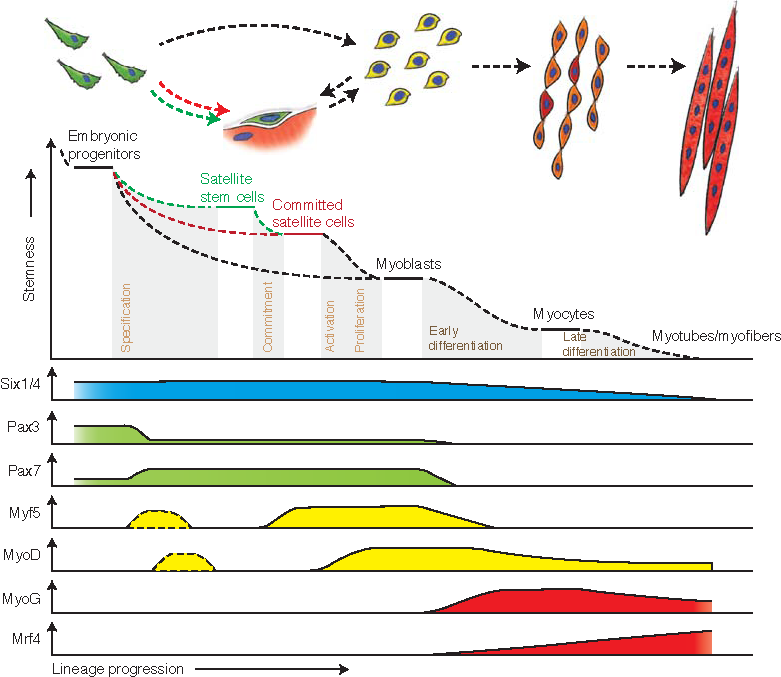
\includegraphics[width=1\textwidth]{figures/bentzinger_myogenesis_tfs.pdf}
%\captionbf{Small caption for Table of Figures}{

%Main caption

%}
%\label{fig:bentzinger_myogenesis_tfs}
%\efig

D'un point de vue g�n�tique, la myogen�se des vert�br�s est coordonn�e en
partie par l'action de $4$ Facteurs de R�gulation Myog�nique (MRF pour
\textit{Myogenic Regulatory Factors}) : MyoD, Myf5, Mrf4 et Myog, qui font
partie de la famille de prot�ines \textit{basic Helix-Loop-Helix} (bHLH) et se
fixent sur les bo�tes E (ou E-box) du type CANNTG.  Ces MRFs sont activ�s
successivement � travers une cascade de r�gulation g�n�tique, et se r�gulent les
uns les autres. Par exemple, Myf5, MRF4 et MyoD peuvent activer MyoD ; Myf5,
MyoD et Mrf4 r�gulent l'expression de Myog ; et Myog peut activer l'expression
de Mrf4 \cite{Naidu1995uq}. En outre, MyoD et Myog peuvent s'auto-activer
\cite{Thayer1989kx}. Enfin, un certain degr� de redondance a �t� observ� entre
Myf5, Mrf4 et MyoD au cours du d�veloppement embryonnaire de la souris, et
l'analyse des embryons KO pour ces g�nes a conduit � la conclusion qu'ils ont
tous la capacit� d'activer la myogen�se � partir de cellules embryonnaires
pluripotentes et d'agir comme des g�nes de d�termination
\cite{KassarDuchossoy2004p823}. 


Ces MRFs sont la cl� de vo�te de la diff�renciation myog�nique. Cependant, la
r�gulation pr�cise du r�seau de g�nes activ�s par les MRFs n�cessite leur
coop�ration avec d'autres facteurs de transcription. En particulier, la liaison
de MyoD � l'ADN n'est pas pr�dictive d'une activit� enhancer
\cite{Cao2010p1805}. Ainsi, \citet{Molkentin1996p646} ont montr� que
l'activation transcriptionnelle par les MRFs est renforc�e par la fonction des
TFs � bo�te MADS MEF$2$. Leur importance a ult�rieurement �t� confirm�e par les
travaux de \citet{Blais2005p809} : en utilisant un grand nombre de g�nes cibles
des MRFs, les auteurs ont cherch� dans leur r�gion promotrice des sites de
liaison sur-repr�sent�s pour les TFs issus de la base de donn�es Transfac. Ils
ont ainsi constat� que l'�l�ment riche en A/T reconnu par MEF2 �tait parmi eux,
et ont confirm� son recrutement � plusieurs de ces sites.  Par ailleurs, un
autre motif d'ADN trouv� comme sp�cifiquement enrichi parmi les promoteurs
cibles des MRFs �tait l'�l�ment \mef (consensus GAAACCTGA), le site de liaison
des hom�oprot�ines Six. Cette s�quence \mef �tait particuli�rement abondante au
sein des promoteurs des g�nes dont l'expression �tait induite de mani�re
significative au cours de la diff�renciation.
% subsection
% la_r_gulation_g_n_tique_les_facteurs_de_r_gulation_myog_nique_ou_mrfs (end)



\subsection{Les hom�oprot�ines Six}
\label{sub:les_hom_oprot_ines_six}

Les hom�oprot�ines Six associ�es aux sites MEF$3$ poss�dent un r�le �tendu au
cours de la myogen�se, et nous en pr�sentons maintenant les d�tails.  Parmi les
6 g�nes appartenant � la famille des hom�oprot�ines Six
  (fig.~\ref{fig:kawakami-six-expression}), \textit{Six$1$} et \textit{Six$4$}
  ont re�u une attention particuli�re dans le contexte de la myogen�se
  squelettique, bien que d'autres membres comme \textit{Six$2$} ou
  \textit{Six$5$} semblent �tre en mesure de compenser partiellement leur perte
  \cite{Relaix2013ve}. Ces deux g�nes se trouvent � proximit� l'un de l'autre
  sur le chromosome $12$ de la souris et sont s�par�s par $100$kb de s�quence
  interg�nique. L'�quipe de Pascal Maire a d�j� identifi� plusieurs fonctions
  cl�s de \textit{Six$1$} dans le lignage musculaire au cours de
  l'embryogen�se, par l'analyse de mod�les de souris d�pourvues de
  \textit{Six$1$} (Six$1$KO) et de Six$1$ et Six$4$ (\sixdko), et par des
  exp�riences de \chip.  L'analyse des embryons \sixdko \cite{Grifone2005vn}
  � E$10$ \cite{Niro2010p3444} et E$18$ \cite{Richard2011ys} a permis
  d'identifier des cibles g�n�tiques directes et indirectes de Six$1,4$, et
  a d�voil� plusieurs fonctions des hom�oprot�ines Six pendant le d�veloppement
  musculaire et la sp�cialisation des fibres musculaires.  

\bfig
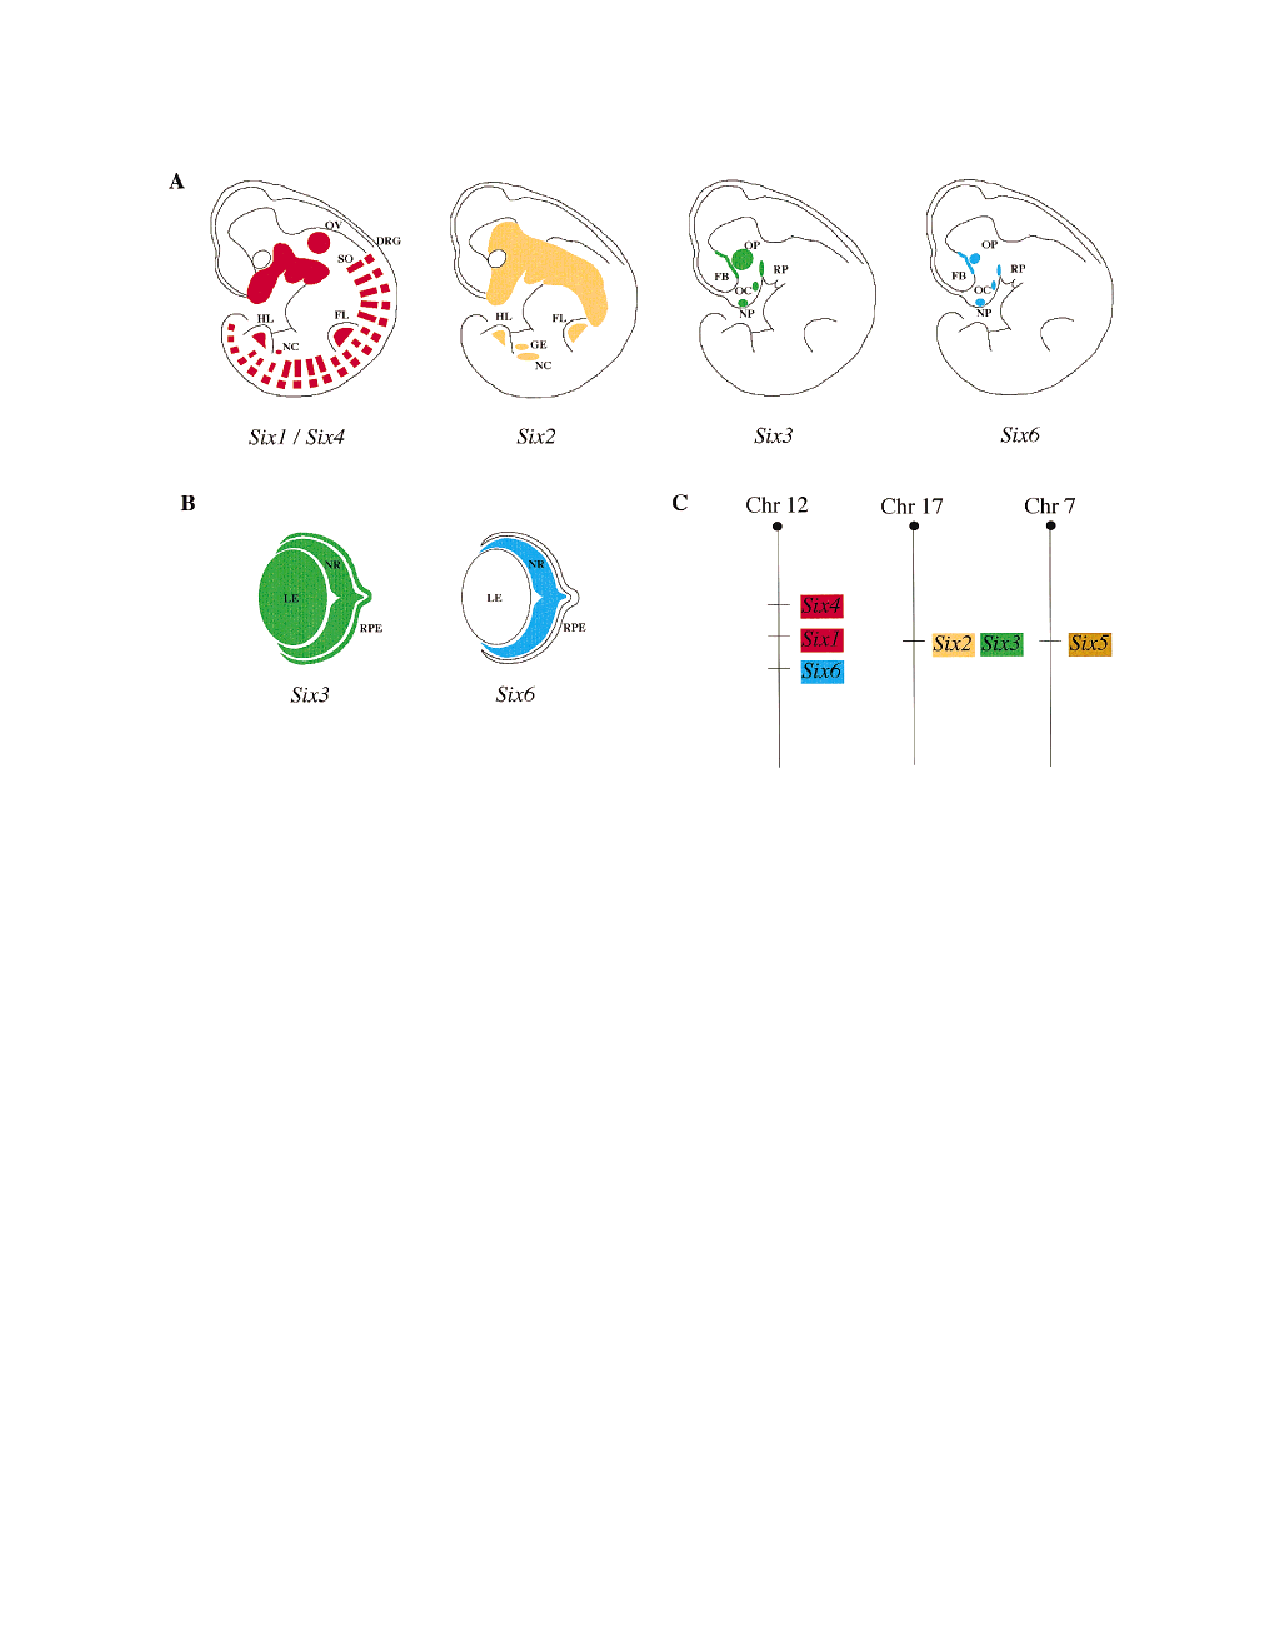
\includegraphics[width=.75\textwidth]{figures/kawakami-six-expression.pdf}
\captionbf{Motifs d'expression et localisation g�nomique des g�nes de la famille Six}{

    Figure tir�e de \cite{Kawakami2000bh}, montrant les motifs d'expression des
    g�nes de la famille Six chez l'embryon (A) et dans l'oeil (B) � E$13.5$.
    Les couleurs similaires refl�tent des motifs d'expression similaires. La
    localisation chromosomique des g�nes est aussi montr�e en (C). 

}
\label{fig:kawakami-six-expression}
\efig


Les principaux points sont les suivants (fig.~\ref{fig:muscle/myogenese_six})
: Six$1$ et Six$4$ sont requis pour la gen�se des prog�niteurs myog�niques
hypaxiaux (\cad ventraux).  En l'absence de Six$1$ et Six$4$, les cellules
ventrales pluripotentes du dermomyotome somitique ne parviennent pas � adopter
un destin de prog�niteur myog�nique et elles n'expriment ni \textit{Pax3} ni
les MRFs. Six$1$ et Six$4$ contr�lent directement l'expression de
\textit{Pax$3$} \cite{Grifone2007p728}, et donc l'engagement des cellules
pluripotentes dermomyotomales dans un destin de prog�niteur myog�nique.  Plus
tardivement, l'expression de \textit{Myf$5$} dans le membre est contr�l�e par
un enhancer \og membre \fg li� par les prot�ines Six$1$ et Six$4$, et cette
liaison est n�cessaire pour permettre l'expression de Myf$5$
\cite{Giordani2007p473}. Par ailleurs, deux enhancers contr�lent sp�cifiquement
l'expression de MyoD au cours de l'embryogen�se et au cours de la r�g�n�ration
du muscle adulte: le \textit{Distal Regulatory Region} ou DRR
\cite{Asakura1995ly} et le \textit{Core Enhancer} ou CE
\cite{Kucharczuk1999zr}. La liaison de ces �l�ments par Six$1$ et Six$4$ a �t�
confirm�e par \chip au cours de l'embryogen�se (\citet{Relaix2013ve}, voir
section \ref{sub:r_gulation_de_myod1_par_les_prot_ines_six}) ainsi que dans des
cultures de cellules satellites \cite{Le-Grand2012qf}, qui sont des cellules
souches du muscle adulte activ�es lors de la r�g�n�ration musculaire.
L'expression de Mrf$4$ n'est pas d�tect�e chez les embryons \sixdko � E$10$
\cite{Grifone2007p728}. Myog est aussi sous le contr�le direct des prot�ines
Six \cite{Spitz1998p3285}. Enfin, les prot�ines Six r�gulent des g�nes
sp�cifiques des fibres glycolytiques de type rapide (voir section
\ref{sub:r_gulation_d_un_lincrna_par_six_dans_le_muscle_adulte}). Par exemple,
la mutation du site MEF$3$ au sein du promoteur de \textit{Aldoa}, g�ne codant
pour une enzyme impliqu�e dans la glycolyse, entra�ne l'abolition de
l'expression d'un transg�ne rapporteur dans des myofibres adultes
\cite{Spitz1997p455}.

\bfig
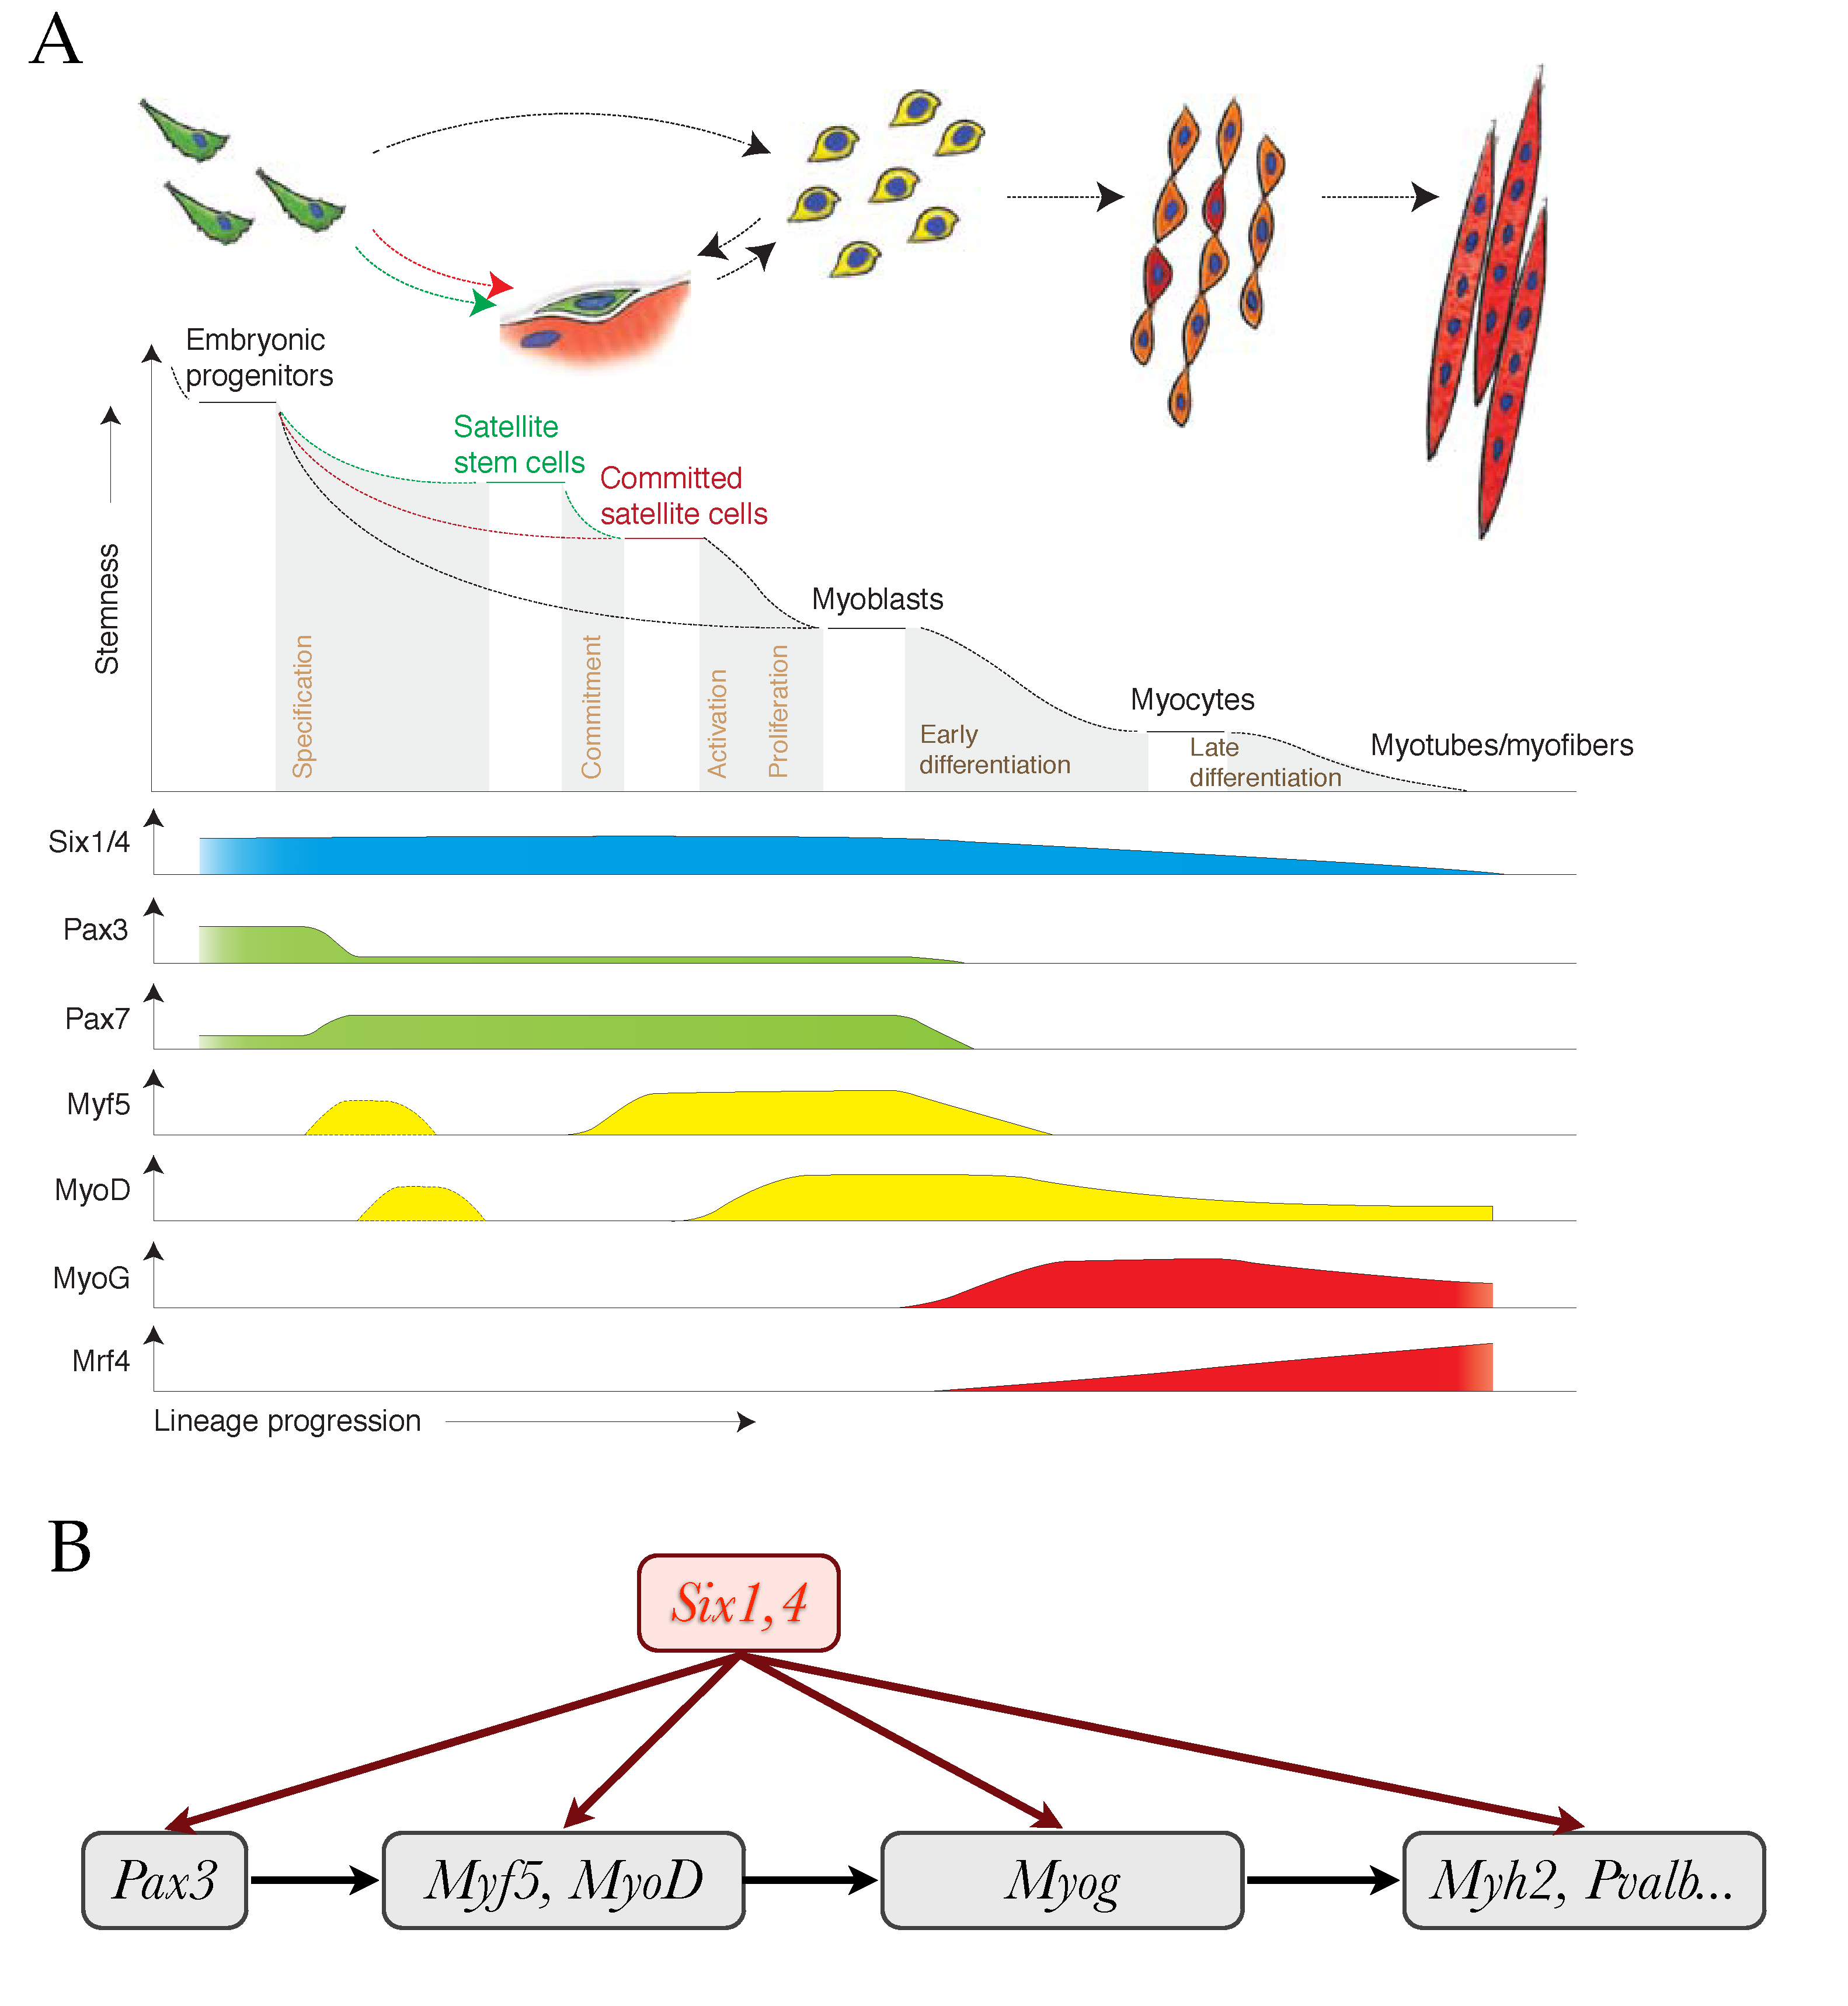
\includegraphics[width=1\textwidth]{figures/muscle/myogenese_six.pdf}
\captionbf{R�le des prot�ines Six au cours de la myogen�se}{

(A) Figure tir�e de \citet{Bentzinger2012ij}. La myogen�se embryonnaire
consiste en plusieurs �tapes de diff�renciation musculaire : la gen�se des
prog�niteurs embryonniques exprimant \textit{Pax3}, leur sp�cification en
myoblastes par l'induction des g�nes de d�termination myog�nique comme
\textit{Myf5} et \textit{Myod1}, la diff�renciation des myoblastes en myocytes
avec l'expression de \textit{Myog} et leur fusion en myotubes qui se
sp�cialisent plus tardivement en fibres de type lentes (oxydatives) ou rapides
(glycolytiques).  On note que les prot�ines Six sont exprim�es continuellement
au cours de ces �tapes (et aussi plus tardivement dans les fibres rapides).

(B) Les hom�oprot�ines Six  interviennent dans la r�gulation de ces diff�rentes
�tapes \invivo en r�gulant les TFs indiqu�s selon une cascade de boucles
\textit{feed-forward}. 

}
\label{fig:muscle/myogenese_six}
\efig

%Ainsi, Six$1$ et Six$4$ contr�lent directement Pax$3$ et tous les MRF, mais ce
%contr�le est spatialement (axe dorso-ventral et axe ant�ro-post�rieur)
%h�t�rog�ne dans l'embryon.




%Par analyse
%bioinformatique, j'ai trouv� deux MEF3 sites dans le noyau activateur et un
%MEF3 site du RRC.  Mutation de ces trois MEF3 des sites aboli par plus de 95%
%l'expression d'un journaliste du transg�ne MyoD dans une souris transg�nique
%essai transitoire � E11.5 dans toutes les lign�es myog�niques (tronc, membres,
%t�te) (Relaix
%2012). 


%Mutations introduites dans le site MEF3 pr�sente dans le
%promoteur myog�nine abolies expression d'une �-galactosidase transg�ne
%rapporteur myog�nine cours de l'embryogen�se (Spitz,1998), et les mutations
%introduites dans le site MEF3 pr�sente dans le promoteur AldolaseA abolis
%l'expression d'un transg�ne rapporteur dans myofibres adultes (Spitz, 1997).
%Par cons�quent, six prot�ines apparaissent comme de bons candidats pour MFR de
%modulation de la r�gulation transcriptionnelle.  N�anmoins, la coop�ration des
%centres de tri et TFS associ�s est loin d'�tre enti�rement comprise, et la
%coop�ration des centres de tri avec non pas un, mais une vari�t� de facteurs de
%transcription, par exemple � diff�rents moments au cours de l'embryogen�se,
%afficher une croissance musculaire natale et pendant la r�g�n�ration du muscle
%adulte est susceptible de se produire sur diff�rents activateurs de g�nes
%cibles.



% subsection les_hom_oprot_ines_six (end)



\FloatBarrier
% section introduction_la_myogen_se (end)

\section{Int�gration de donn�es bioinformatiques et exp�rimentales sur le muscle} 
\label{sec:integration_de_donn_es_bioinformatiques_et_exp_rimentales_sur_le_muscle}

La premi�re �tape de notre collaboration avec l'�quipe de P. Maire a �t� de
construire un mod�le de motif pour les sites de fixation \mef associ�s aux
prot�ines \sixd chez la souris. Un tel motif, qui n'existait jusqu'alors pas,
permet de r�aliser des pr�dictions pr�cises, et nous discuterons apr�s de leur
v�rification.  Par ailleurs, nous avons r�cup�r� de nombreuses donn�es
exp�rimentales dans la litt�rature sur la diff�renciation musculaire (\chipseq,
RNAseq, donn�es �pig�n�tiques\ldots) et les avons int�gr�es au syst�me de
visualisation de UCSC (pr�sent� en introduction, section
\ref{sub:outils_visualisation}).  L'int�gration de ces multiples donn�es permet
d'appr�hender facilement et rapidement les ph�nom�nes de r�gulation ayant lieu
lors de la diff�renciation musculaire � l'�chelle locale de g�nes d'int�r�t
comme � l'�chelle globale g�nomique en croisant les donn�es. 


\subsection{Obtention d'une PWM optimale pour MEF3}
\label{sub:obtention_d_une_pwm_optimale_pour_mef3}

\begin{table}[!t]
\centering
%\resizebox{8cm}{!} {
\begin{tabular}{|l|l|}
\hline
\multicolumn{2}{|c|}{S�quences positives d'apprentissage}\\
\hline
Myog & \texttt{GAAACCTGA} \\
Pax3 & \texttt{GAAATCTAA} \\
Myf5 & \texttt{GTAACTGGA} \\
Myod-DRR & \texttt{GAAACCGGA} \\
Mlc-hox & \texttt{GTAATTTAA} \\
Atp2a1-1 & \texttt{GTAACTGGA} \\
Atp2a1-2 & \texttt{GTAACCTGA} \\
Tnnc2 & \texttt{GAAATTTAA} \\
Nrk & \texttt{GCAAGGCGA} \\
Sarcalumenin & \texttt{GGAACTTGA} \\
Myl1-2 & \texttt{GAAATTGAA} \\
Ifitm3 & \texttt{GTAATTTGA} \\
Mybph-2 & \texttt{GAAATCTGA} \\
Myeov2 & \texttt{GAAACTTGA} \\
\hline
\end{tabular}
\begin{tabular}{|l|l|}
\hline
\multicolumn{2}{|c|}{S�quences positives test}\\
\hline
Aldoa & \texttt{GAAACCTGA} \\
Ato & \texttt{GTCATTTGA} \\
Kcne1l & \texttt{GATAACGGA} \\
Myf5 & \texttt{GAAATTTAA} \\
Pax3-1 & \texttt{GAAATGTAA} \\
Pax3-2 & \texttt{GTTACTGGA} \\
Pvalb & \texttt{GTAACCTGA} \\
Utrophine & \texttt{GTCACCTGA} \\
Na-K-ATPase & \texttt{GCAACCTGA} \\
Myf5-2 & \texttt{GCAACCTGA} \\
Myf5-sat & \texttt{GAAATCTGA} \\
Lbx1 & \texttt{GCCACCTGA} \\
MCK & \texttt{GACACCCGA} \\
IgfBp5 & \texttt{GCAATTTGA} \\
Troponine-C & \texttt{GTAACCTGA} \\
Sarcalumenin & \texttt{GGAACTTGA} \\
Nrk & \texttt{GCAAGGCGA} \\
Tp4 & \texttt{GCAAGCAGA} \\
\hline
\end{tabular}
%}
\captionbf{Sites \mef positifs}{ 
    
    Le tableau de gauche correspond aux $14$ sites conserv�s chez les
    mammif�res que nous avons utilis�s pour l'apprentissage de la PWM \mef, et
    le tableau de droite aux sites utilis�s comme un ensemble test ind�pendant
    de Vrais Positifs dans la courbe ROC de la figure
    \ref{fig:muscle/roc-mef3}.

}
\label{tab:mef3_pos}
\end{table}

\begin{table}[!t]
\centering
%\resizebox{8cm}{!} {
\begin{tabular}{|l|l|}
\hline
\multicolumn{2}{|c|}{S�quences n�gatives}\\
\hline
myf5-1 & \texttt{GACAGTGGA} \\
myf5-2 & \texttt{GTAACCTCA} \\
myf5-3 & \texttt{GTAACTGGG} \\
pax3-1 & \texttt{GGAACTTGA} \\
pax3-2 & \texttt{GTATTAATA} \\
pax3-3 & \texttt{GGATAAAGA} \\
pax3-4 & \texttt{GCTAATTGA} \\
pax3-5 & \texttt{GAAAGATTA} \\
pax3-6 & \texttt{GCTCTCTGA} \\
pax3-7 & \texttt{GAGCCCTGA} \\
pvalb-1 & \texttt{GCACAATGA} \\
pvalb-2 & \texttt{GCAGGCTGA} \\
unknown-1 & \texttt{GCAATCTGA} \\
unknown-2 & \texttt{GAGTCCTGA} \\
\hline
\end{tabular}
%}
\captionbf{Sites \mef n�gatifs}{ 
    
    Sites n�gatifs utilis�s comme Faux Positifs dans la courbe ROC de la figure
    \ref{fig:muscle/roc-mef3}.

}
\label{tab:mef3_neg}
\end{table}

Avant notre arriv�e au laboratoire de P. Maire, il n'existait pas de PWM pour
\mef, et les pr�dictions �taient faites sur la base de la proximit� au
consensus GAAACCTGA issu du promoteur de Myog. Nous avons donc d�cid� de
construire un motif pour les sites de fixation \mef associ�s aux prot�ines
\sixd. Pour ce faire, nous avons utilis� le fait qu'un certain nombre de sites
de fixation avaient d�j� �t� test�s par retard sur gel (EMSA ou
\textit{Electrophoretic Mobility Shift Assay}), exp�rience permettant de
d�tecter une interaction entre une prot�ine et de l'ADN, que ce soit dans la
litt�rature ou au sein du laboratoire de P.  Maire. Ces exp�riences ont permis
de d�finir $32$ sites positifs (table \ref{tab:mef3_pos}) et $14$ sites
n�gatifs (table \ref{tab:mef3_neg}). Les
sites positifs ont ensuite �t� partag�s en un ensemble d'apprentissage compos� de $14$
s�quences pour lesquelles les s�quences orthologues chez les autres mammif�res
�taient disponibles, et en un ensemble \og test \fg ind�pendant de $18$ sites.

\bfig
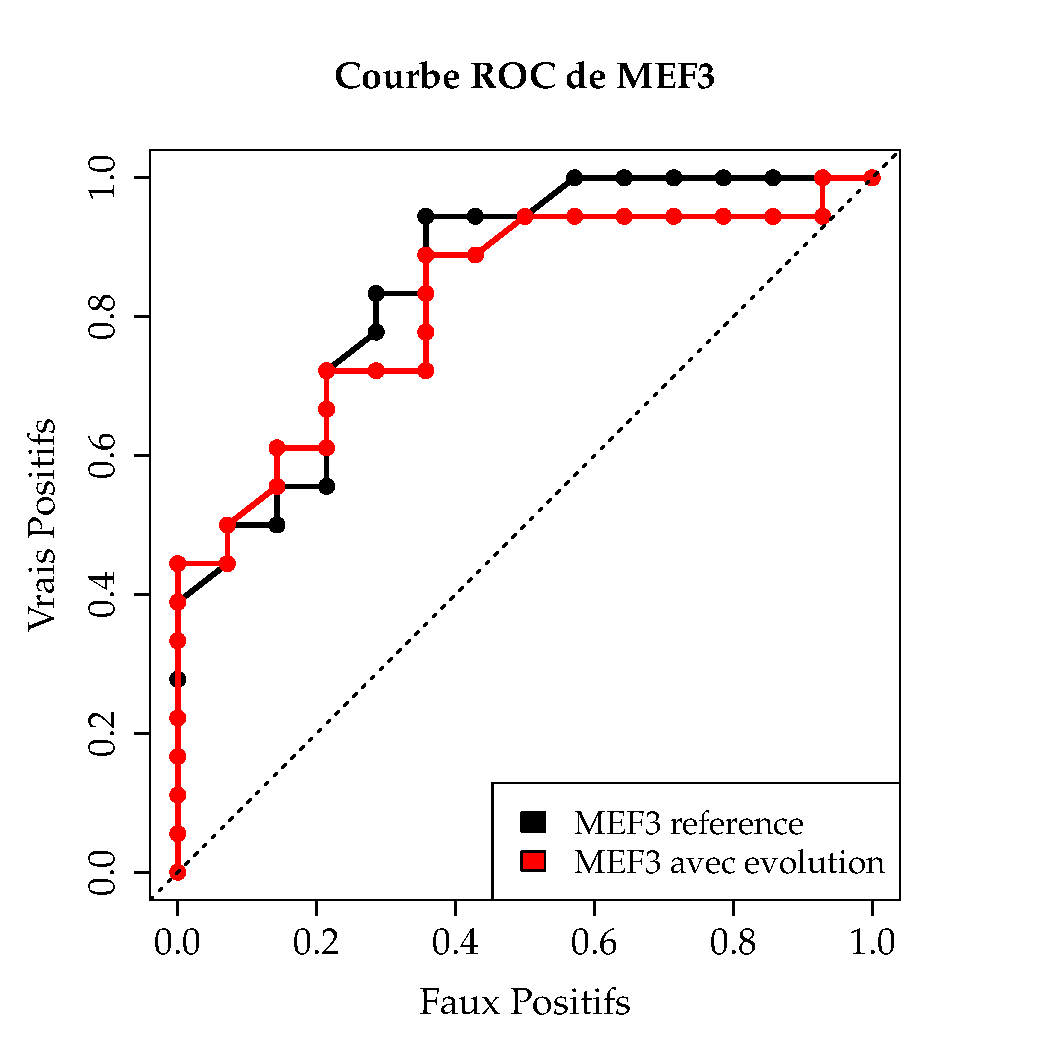
\includegraphics[width=0.8\textwidth]{figures/muscle/MEF3-roc-on-posnotlearned/roc.pdf}
\captionbf{Courbe ROC de MEF3}{

Nous comparons la capacit� de classification de sites MEF3 positifs ou n�gatifs
(par EMSA) pour diff�rentes PWMs : chaque point repr�sente le taux de Vrais
Positifs et de Faux Positifs pr�dits au-dessus d'un seuil de d�tection donn�.
Les PWMs ont �t� obtenues � partir de $14$ sites positifs diff�rents des sites
utilis�s dans la classification, soit en utilisant les sites orthologues chez
d'autres mammif�res et un mod�le d'�volution (courbe rouge) ou en utilisant
juste les sites de l'esp�ce de r�f�rence (courbe noire). Dans chaque cas, les
param�tres (seuil de g�n�ration fixant la valeur du pseudo-count, mod�le
d'�volution) ont �t� vari�s et seule la meilleure courbe ROC est montr�e. Le
cas avec �volution est meilleur � haut seuil (inflexion initiale pour
$S_s>6.5$bits) que le mod�le sans �volution. Les param�tres associ�s sont
: $S_g=8.7$ bits et mod�le Halpern-Bruno pour le cas avec �volution, $S_g=12$
bits pour le cas r�f�rence.

}
\label{fig:muscle/roc-mef3}
\efig


 Nous avons alors cherch� la PWM apprise sur l'ensemble d'apprentissage qui
 distinguait le mieux les sites positifs de l'ensemble test des sites n�gatifs.
 Ces derniers ayant �t� choisis en fonction de leur resemblance avec le site
 consensus de \mef sur le promoteur de \textit{Myog}, le fait de trouver une
 PWM distinguant sites positifs des n�gatifs permet v�ritablement d'am�liorer
 l'approche heuristique.  Nous avons g�n�r� deux types de PWMs : une PWM \og
 r�f�rence \fg apprise sur les $14$ s�quences d'apprentissage, et une PWM \og
 avec �volution \fg apprise avec Imogene � partir des alignements des s�quences
 d'apprentissage avec leurs orthologues.  Le seuil de g�n�ration des PWMs a �t�
 vari� entre $7$ et $12$ bits, et les deux mod�les d'�volution
 (\textit{Felsenstein} et \textit{Halpern-Bruno}) ont �t� utilis�s. Pour chaque
 PWM, une courbe ROC (pour \textit{Receiver Operating Characteristic}) peut
 �tre construite indiquant pour diff�rents seuils de d�tection $S_s$ la
 proportion de s�quences positives d�tect�es dans l'ensemble test (Vrais
 Positifs
 %ou TPs pour \textit{True Positives}
 ) et la proportion de s�quences n�gatives d�tect�es (Faux Positifs ou FPs).
 Nous montrons en figure \ref{fig:muscle/roc-mef3} les meilleures courbes ROC
 obtenues pour les cas r�f�rence et avec �volution. Les deux courbes sont
 relativement similaires et permettent de d�tecter $45\%$ des sites positifs
 sans d�tecter aucun n�gatif pour un seuil de l'ordre de $S_g=7$ bits. La PWM
 avec �volution (fig.~\ref{fig:muscle/mef3evolh6})
 %, nomm�e MEF3evolh$6$, 
 montre une l�g�re am�lioration du signal � haut seuil (petits FPs) par rapport
 � la PWM r�f�rence, et nous avons donc utilis� celle-ci dans la suite de notre
 travail. 

 \bfig
 \includegraphics[width=1\textwidth]{figures/muscle/mef3evolh6.pdf}
 \captionbf{PWM \mef obtenue avec le mod�le d'�volution}{
 
 
 }
 \label{fig:muscle/mef3evolh6}
 \efig


% subsection obtention_d_une_pwm_optimale_pour_mef3 (end)


\subsection{Obtention de donn�es � partir de la litt�rature et int�gration au visualisateur de UCSC}
\label{sub:obtention_de_donn_es_partir_de_la_litt_rature_et_int_gration_ucsc}

La litt�rature regorge de donn�es publi�es obtenues dans diff�rents mod�les
musculaires, que ce soit des cultures de cellules \cd,  lign�e cellulaire de
myoblastes de souris couramment utilis�e pour mod�liser la diff�renciation
musculaire, ou dans des tissus provenant de la dissection de muscles
squelettiques chez l'embryon ou chez l'adulte. N�anmoins, il n'existe pas
d'outil centralisant ces donn�es sp�cifiques au muscle. Nous avons donc
r�cup�r� ces donn�es et les avons int�gr�es sur l'outil de visualisation Genome
Browser de UCSC afin de faciliter l'analyse des �v�nements de r�gulation au
cours de la diff�renciation musculaire (fig.~\ref{fig:muscle/UCSC_myod1}).


\bfigp
\includegraphics[width=1\textwidth]{figures/muscle/UCSC_myod1.pdf}
\captionbf{Visualisation de donn�es musculaires sur UCSC}{

    Capture d'�cran du navigateur de UCSC (UCSC Genome Browser,
    \url{http://genome.ucsc.edu}) montrant le locus de \textit{Myod1} et
    incluant un certain nombre des donn�es que nous avons recueillies.
    L'int�gration des donn�es permet de conduire rapidement plusieurs analyses
    sur la r�gulation g�n�tique (voir texte principal). Les cadres color�s
    indiquent des r�gions de r�gulation potentielles fix�es par MyoD (cadre
    pourpre avec Pax$3$ et Pax$7$, vert avec Smad3), ainsi que le \textit{Core
    Enhancer} CE (cadre rouge de gauche) et le \textit{Distal Regulatory
    Region} DRR (cadre rouge de droite). L'ensemble de ces enhancers constitue
    un \textit{super enhancer} (voir \ref{sub:les_super_enhancers} et
    \citet{Whyte2013tg}).

}
\label{fig:muscle/UCSC_myod1}
\efigp


Parmi ces donn�es figurent d'abord des exp�riences issues du projet ENCODE
(pr�sent� dans l'introduction en section \ref{sub:projet_encode}). Celles-ci
sont de plusieurs types et ont �t� obtenues par des laboratoires diff�rents. Il
y a notamment des donn�s RNAseq, quantifiant pr�cis�ment la transcription d'ARN
dans diff�rentes conditions (\cd � Caltech, muscle squelettique � University of
Washington ou UW), des donn�es d'hypersensibilit� � la digestion par DNAseI
(voir \ref{sub:chip_DNAseI}) en muscle adulte (UW) ainsi que diverses donn�es
de \chipseq de TFs en \cd (Caltech).  Parall�lement, nous avons obtenu
plusieurs donn�es � partir de la litt�rature. Par exemple, nous avons recueilli
les donn�es \chipseq de \citet{Asp2011p2370} pour $10$ marques �pig�n�tiques
sur les histones de cellules \cd cultiv�es en milieu de prolif�ration (MB pour
myoblastes) et en milieu de diff�renciation (MT pour myotubes). Nous avons
aussi recueilli des donn�es \chipseq pour divers TFs impliqu�s dans la
diff�renciation musculaire : le TF ma�tre MyoD en \cd MB et MT
\cite{Cao2010p1805}, les TFs Pax$3$ et Pax$7$ marquant respectivement les
prog�niteurs embryonnaires et les cellules satellites, ou prog�niteurs adultes,
obtenus dans des myoblastes primaires \cite{Soleimani2012p3753}, le TF Smad$3$
associ� � la voie TGF-$\beta$ en MT \cite{Mullen2011p3259}, le TF Msx$1$
permettant le recrutement du groupe Polycomb associ� aux marques r�pressives
H$3$K$27$me$3$ en \cd MB \cite{Wang2011p2929}, ou encore le TF Sox$6$ impliqu�
dans l'inhibition des g�nes sp�cifiques des fibres lentes lors de la
diff�renciation terminale en myoblastes primaires � E$18$ \cite{An2011p2926}.
Par ailleurs, certains TFs n'ont pour le moment �t� �tudi�s que par des
exp�riences de \chipchip � la r�solution et l'�tendue limit�e : le TF Gli
associ� � la voie de signalisation \textit{Sonic hedgehog} (SHH), dont les
donn�es ont �t� obtenues dans le bourgeon de membre d'embryons � E$11.5$
\cite{Vokes2008p1808}, ou encore le TF Six$1$ en \cd MB et MT
\cite{Liu2010p588}. Dans ce dernier cas, les donn�es ne couvrent que $17\%$ du
g�nome et poss�dent une faible r�solution ($\sim 1$kb) : elles sont donc
seulement compl�mentaires aux pr�dictions obtenues en utilisant la PWM MEF$3$
introduite pr�c�demment, car elles confirment la fixation de Six$1$ sur
certains des sites pr�dits (mais n'infirme pas l'absence de fixation des
prot�ines de la famille Six sur les autres sites).\\

Nous pr�sentons en figure \ref{fig:muscle/UCSC_myod1} un exemple montrant la
visualisation d'une partie des donn�es recueillies dans le cas du locus de
\textit{Myod$1$}, g�ne associ� aux prot�ines MyoD. Des informations sur la
position g�nomique et les transcrits pr�sents au sein du locus sont d'abord
donn�es dans la partie sup�rieure. Puis les pistes suivantes indiquent diverses
exp�riences, avec la nomenclature suivante : MB pour myoblaste (avec parfois le
pourcentage de confluence des cellules en culture), MT pour myotube (avec
parfois le temps pass� en milieu de diff�renciation), SkMuscle $8$w pour muscle
squelettique adulte � $8$ semaines post-natales et GM pour \textit{Growth
Medium}.  Les premi�res pistes de donn�es (en brun) sont issues du projet
ENCODE, les pistes suivantes (en noir) indiquent les coordonn�es des pics
\chipseq des marques �pig�n�tiques des histones ainsi que de divers TFs.  Les
pistes bleues pour Pax$3$ et Pax$7$ indiquent les donn�es brutes du nombre de
s�quences de \chipseq par nucl�otide, les segments pourpres indiquant les pics.
On montre aussi le contr�le de cette exp�rience (input) auquel les donn�es sont
compar�es pour d�finir les pics. Ainsi, le pic des donn�es brutes de Pax$3$
dans la partie droite de la piste n'est pas d�tect� comme un pic authentique
car les donn�es contr�le y poss�dent aussi un pic.

Prises ensemble, ces donn�es permettent d'appr�hender la r�gulation du g�ne
\textit{Myod$1$} au cours de la diff�renciation musculaire. D'abord,
\textit{Myod$1$} est transcrit au cours de la diff�renciation des cellules \cd
(d�tection d'ARN par RNAseq, traces de PolII marquant la transcription) mais
son expression est plus faible en muscle adulte, soit longtemps apr�s la
diff�renciation. Le g�ne est dans une r�gion de chromatine ouverte (DNAseI HS),
et c'est aussi le cas pour plusieurs r�gions alentour. Les pics de DNAseI HS
sont notamment corr�l�s aux pics de PolII ainsi qu'� d'autres TFs comme
MyoD\footnote{Il est effectivement connu que \textit{Myod1}
s'autor�gule~\cite{Thayer1989kx}}, Six$1$, Msx$1$, Pax$3$ ou encore Pax$7$, et
� des marques epig�n�tiques \og activatrices \fg comme les m�thylation
d'histone H$3$K$4$me$1$, H$3$K$4$me$2$ et H$3$K$4$me$3$ ou l'ac�tylation
H$3$K$9$Ac, qui sont toutes renforc�es au cours de la diff�renciation (passage
de MB � MT).  Le fait que l'on observe des pics de PolII hors des r�gions
transcrites est d� � l'interaction entre des r�gions de r�gulation contenant
plusieurs TFs et le promoteur du g�ne r�gul� (ici \textit{Myod1}) fixant la
polym�rase. Ces donn�es pointent donc vers l'existence de multiples r�gions de
r�gulation � la chromatine ouverte et interagissant avec le promoteur de
\textit{Myod$1$}. Plus pr�cis�ment, on trouve de gauche � droite : une r�gion
fixant Pax$3$, Pax$7$, Msx$1$ et MyoD en diff�renciation tardive qui pourrait
par exemple �tre impliqu�e dans la diff�renciation des cellules satellites
(cadre pourpre), plusieurs r�gions fixant Smad$3$ et MyoD pouvant peut-�tre
servir � int�grer des signaux TGF-$\beta$ (cadres verts), ainsi que deux
r�gions r�gulatrices connues (cadres rouges), l'une \cite{Kucharczuk1999zr}
fixant MyoD, Six$1$ et Msx$1$ tout au long de la diff�renciation et poss�dant
un site MEF$3$ conserv� (le CE de MyoD, impliqu� dans la diff�renciation des
prog�niteurs embryonnaires), et l'autre \cite{Asakura1995ly} fixant Six$1$ et
MyoD en MT (le DRR, impliqu� chez l'embryon ainsi que dans le muscle adulte).
Ces enhancers semblent donc avoir diff�rent r�les dans l'activation de
\textit{Myod$1$} et la mise en place de la myogen�se. On notera pour finir que
l'ensemble de ces r�gions de r�gulation, � forte densit� de \chipseq pour le TF
ma�tre MyoD et associ�es � des marques �pig�n�tiques extensives, a �t� d�fini
ailleurs comme un \textit{super-enhancer} (voir \ref{sub:les_super_enhancers}
et \citet{Whyte2013tg}).\\


L'int�gration des donn�es exp�rimentales et bioinformatiques li�es � la
r�gulation du ph�notype musculaire permet ainsi de visualiser rapidement la
r�gulation possible d'un g�ne et de proposer des hypoth�ses de m�canismes
sous-jacents, qu'il s'agit ensuite de valider exp�rimentalement. Nous avons pu
partager la session UCSC contenant ces diff�rentes donn�es avec nos
collaborateurs au sein de l'�quipe de P. Maire, qui ont maintenant la
possibilit� de croiser et interpr�ter rapidement un grand nombre de donn�es
publi�es ainsi que de donn�es obtenues au cours de cette th�se.

% subsection obtention_de_donn_es_partir_de_la_litt_rature_et_int_gration_ucsc (end)

\section{Pr�dictions et validations de la r�gulation par Six} 
\label{sec:pr_dictions_et_validations_de_la_r_gulation_par_six}

Plusieurs pr�dictions r�alis�es gr�ce � la PWM \mef ont �t� r�alis�es et
valid�es exp�rimentalement, nous en pr�sentons ici deux majeures.

\subsection{R�gulation de \textit{Myod1} par les prot�ines Six chez l'embryon de souris}
\label{sub:r_gulation_de_myod1_par_les_prot_ines_six}

\bfig
\includegraphics[width=1\textwidth]{figures/muscle/myod_ce_drr_sequences.pdf}
\captionbf{Pr�diction de sites \mef sur les s�quences r�gulatrices CE et DRR de \textit{Myod1}}{

    S�quences correspondant aux r�gions r�gulatrices CE et DRR de
    \textit{Myod1}.  Trois sites \mef ont �t� pr�dits � des scores respectifs
    de $7$ bits pour le premier du CE (CE$1$) et $11.1$ bits pour le deuxi�me
    du CE (CE$2$) et celui du DRR. Le seuil de $7$ bits correspond au seuil
    minimal trouv� en fig. \ref{fig:muscle/roc-mef3} comme discernant positifs
    de n�gatifs. Les sites E-Box, Pitx et Pax3 indiqu�s correspondent � des
    sites d�j� valid�s. Les s�quences soulign�es correspondent aux bo�tes LS$4$
    et LS$15$ de l'exp�rience de \textit{Linker-Scanner Mutagenesis} du CE
    humain r�alis�e par \citet{Kucharczuk1999zr} et sont requises pour
    l'expression dans les lign�es musculaires.

}
\label{fig:muscle/myod_ce_drr_sequences}
\efig

Nous avons d'abord r�alis� des pr�dictions de sites \mef sur deux enhancers
connus de \textit{Myod1}, le \textit{Core Enhancer} CE et le \textit{Distal
Regulatory Region} DRR, qui ont �t� publi�es dans l'article
\citet{Relaix2013ve} paru dans \textit{Plos Genetics}. Les pr�dictions ont �t�
r�alis�es avec un seuil de $7$ bits\footnote{\label{foot:seuil}Il faut noter
que le seuil utilis� pour afficher les sites \mef conserv�s dans le navigateur
de UCSC en figure \ref{fig:muscle/UCSC_myod1} est plus �lev� ($10.5$ bits). En
effet, � l'�chelle g�nomique, il y a une tr�s grande quantit� de sites
n�gatifs, et il faut donc aller vers les petits taux de Faux Positifs (ou les
hauts seuils de d�tection) pour assurer un filtrage du bruit suffisant : par
exemple, on trouve un site non conserv� tous les $2^7 \sim 128$ bp pour un
seuil de $7$ bits, contre $2^{10.5} \sim 1500$ pour un seuil de $10.5$ bits. En
ajoutant le crit�re de conservation, ces quantit�s sont plus petites, et le
seuil de $7$ bits para�t raisonnable pour des pr�dictions sur des s�quences de
petite taille $\sim200$ bp.  } correspondant au seuil de distinction optimal de
sites \mef positifs et n�gatifs introduit en figure \ref{fig:muscle/roc-mef3}.
Nous avons ainsi d�tect� $2$ sites \mef sur le CE et $1$ sur le DRR que nous
montrons en figure \ref{fig:muscle/myod_ce_drr_sequences}. Sur le CE, les deux
sites recoupent en partie des �l�ments essentiels � l'expression \invivo du CE
humain dans les cellules musculaires myotomales de la souris
\cite{Kucharczuk1999zr}. Nous montrons par ailleurs d'autres sites d�tect�s
dans des travaux pr�c�dents \cite{Lhonore2010p3969,Kucharczuk1999zr}  : les
sites Pitx$2$ et Pax$3$ dans le CE, ou encore les E-box dans le CE et le DRR.\\


\bfigp
\includegraphics[width=1\textwidth]{figures/muscle/myod_ce_drr_mutations_relaix.pdf}
\captionbf{Validation des sites \mef pr�dits dans les �l�ments r�gulateurs de \textit{Myod1}}{

    Figure pr�sent�e dans l'article \citet{Relaix2013ve}. Plus de d�tails sont
    donn�s dans le texte principal. (A) Exp�rience de \chip montrant que les
    prot�ines Eya, cofacteurs de Six$1$ et Six$4$, sont recrut�es au niveau du
    CE et du DRR. (B) Exp�riences de retard sur gel (EMSA) montrant  que Six$1$
    et Six$4$ interagissent avec les sites pr�dits sur les enhancers.  (C)
    Sch�ma des transg�nes wild-type et mut�s en sites \mef. (D) Coloration au
    X-Gal d'embryons � E$12.5$ porteurs de transg�nes des s�quences wild-type
    (a, b, c) et mutantes (d, e, f), montrant l'abolition de l'expression du
    g�ne rapporteur lorsque les sites \mef sont mut�s.  (E) Analyse de
    l'expression de MyoD par immunohistochimie et du rapporteur LacZ par
    coloration X-Gal dans les coupes indiqu�es par un trait noir chez les
    embryons c, d, e et f au niveau du thorax (Th) et des yeux (Eye). On note
    l'absence d'expression du transg�ne mut� dans les cellules exprimant MyoD.

}
\label{fig:muscle/myod_ce_drr_mutations_relaix}
\efigp

La validation de ces pr�dictions est pr�sent�e en figure
\ref{fig:muscle/myod_ce_drr_mutations_relaix}. Tout d'abord, il est montr� par
retard sur gel que les prot�ines Six$1$ et Six$4$ se fixent effectivement sur
les s�quences pr�dites (fig.~\ref{fig:muscle/myod_ce_drr_mutations_relaix}B).
Dans cette exp�rience, des oligonucl�otides marqu�s par la radioactivit�
contenant le site \mef consensus GAAACCTGA du promoteur de Myog sont incub�s
avec les prot�ines Six$1$ et Six$4$ synth�tis�es \invitro (colonne $1$). On
ajoute ensuite des oligonucl�otides non marqu�s en exc�s d'un facteur $60$ ou
$300$ et contenant le site \mef de Myog (contr�le positif, colonnes $2$ et
$3$), les sites \mef du DRR (colonnes $4$ et $5$) et du CE (site $1$ : colonnes
$6$ et $7$, site $2$ : colonnes $8$ et $9$), ou le site NFI  du promoteur de
Myog (contr�le n�gatif, colonne $10$, exc�s de $300$). Ensuite, il est montr�
que la mutation des sites \mef abolit l'expression d'un rapporteur \invivo de
l'activit� des enhancers par transgen�se. Pour cela, deux constructions ont �t�
r�alis�es, contenant le CE, le DRR ainsi que le promoteur PRR (\textit{Proximal
Regulatory Region}) de \textit{Myod1} en amont du g�ne rapporteur LacZ, avec ou
sans mutations au niveau des $3$ sites \mef pr�dits
(fig.~\ref{fig:muscle/myod_ce_drr_mutations_relaix}C). Ces constructions ont
�t� introduites dans des embryons par transgen�se transitoire, et ceux-ci sont
pr�lev�s � E$12.5$ puis l'expression de LacZ est r�v�l�e par coloration au
X-Gal (fig.~\ref{fig:muscle/myod_ce_drr_mutations_relaix}D). Au total, $6$
transg�nes \textit{wild-type} sur $10$ expriment le rapporteur
LacZ\footnote{Cette variation d'expression est notamment due au fait qu'il est
    difficile de contr�ler le nombre de transg�nes ins�r�s dans le g�nome. Les
    diff�rents embryons montr�s en figure
    \ref{fig:muscle/myod_ce_drr_mutations_relaix}D,E sont repr�sentatifs des
diff�rents taux d'insertions obtenus.}  avec un motif d'expression st�r�otyp�
($3$ d'entre eux sont montr�s sur la figure). Dans le cas des transg�nes mut�s,
$3$ sur $8$ expriment tr�s l�g�rement LacZ, ils sont tous montr�s sur la
figure. Enfin, des sections r�alis�es au niveau de la t�te et du thorax montre
que l'expression du rapporteur du transg�ne \textit{wild-type} r�capitule le
motif d'expression du g�ne \textit{Myod1} endog�ne, alors que pour les
transg�nes mut�s l'expression est tr�s rare. Ainsi, les prot�ines MyoD,
Mef$2$, Pitx, etc., pr�sentes dans les cellules myog�niques sont incapables
d'activer les r�gions r�gulatrices mut�es dans les sites \mef, sugg�rant
qu'elles sont incapables de se fixer � l'ADN.
  
  %Ainsi, le nombre de transg�nes ins�r�s dans les embryons positifs
  %(X-Gal+) varie entre $3$ et $34$, alors que pour les n�gatifs il varie entre
  %$1$ et $14$. 
%The number of transgenes inserted was 23 (f), 39
%(d) and 40 (e) for X-Gal+ embryos, and from 1 to 51 for X-Gal2 embryos. F-

% subsection r_gulation_de_myod1_par_les_prot_ines_six (end)

\subsection{R�gulation d'un lincRNA par Six dans le muscle adulte}
\label{sub:r_gulation_d_un_lincrna_par_six_dans_le_muscle_adulte}

Nous pr�sentons maintenant un travail r�alis� en collaboration avec Iori
Sakakibara de l'�quipe de P. Maire.

\subsubsection{Contexte g�n�ral}

\bfigp
\includegraphics[width=1\textwidth]{figures/muscle/UCSC_lincMYH.pdf}
\captionbf{Visualisation du locus des myosines sur UCSC}{

    Le locus des myosines s'�tend sur $300$ kb sur le chromosome $11$ de la
    souris. Au sein de ce locus ce trouve un long ARN non codant (linc-RNA),
    AK$010044$ ou linc-MYH. Ce lincRNA est transcrit dans le muscle
    squelettique (RNAseq), o� il se trouve au sein d'un r�gion de chromatine
    ouverte (DNAseI HS). La r�gion est marqu�e par une forte r�gulation
    �pig�n�tique lors de la diff�renciation des \cd : apparition de marques
    d'activation (H$3$K$4$me et diverses ac�tylations) et disparition de marque
    inhibitrices (H$3$K$27$me$3$), ces changements �tant corr�l�s avec des
    traces �tendues sur le locus de PolII.  Linc-MYH est entour� de r�gions de
    r�gulation putatives contenant les TFs MyoD, Six$1$, Smad$3$ et Sox$6$.
    Ici, nous nous sommes concentr�s sur la r�gion directement en amont du TSS
    de lincMYH (indiqu�e par une fl�che rouge), contenant des traces \chipseq
    pour MyoD et Six$1$ en MT, ainsi que plusieurs sites MEF$3$ conserv�s
    � haut score.

}
\label{fig:muscle/UCSC_lincMYH}
\efigp

Les prot�ines Six poss�dent un r�le important dans la sp�cialisation des fibres
musculaires de type rapide (ou glycolytiques) lors de la diff�renciation
tardive~\cite{Niro2010p3444}. De plus, dans le muscle adulte, Six$1$ est
exprim� de mani�re plus importante dans les noyaux des fibres adultes que dans
ceux des fibres lentes. Le ph�notype rapide est marqu� par l'expression de
g�nes \og rapides \fg, dont les troponines \textit{Tnnt$3$}, \textit{Tnni$2$}
et \textit{Tnnc$2$} ou les myosines \textit{Myh$2$}, \textit{Myh$1$} et
\textit{Myh$4$}. La question concernant le r�le exact des prot�ines Six lors de
cette sp�cialisation est encore ouverte .\\

Nous avons concentr� notre �tude sur le \og cluster myosines \fg s'�tendant sur
$300$ kb dans le chromosome $11$ de la souris, et contenant les myosines
\textit{Myh$3$} (embryonnaire), \textit{Myh$2$} (rapide de type $2$A),
\textit{Myh$1$} (rapide de type $2$X), \textit{Myh$4$} (rapide de type $2$B),
\textit{Myh$8$} (p�rinatale) et \textit{Myh$13$} (extra-oculaire). Nous
montrons en fig.~\ref{fig:muscle/UCSC_lincMYH} une partie de ce locus. Nous
nous sommes demand�s si les prot�ines Six pouvaient r�guler directement les
myosines de type rapide au niveau de ce locus. La concentration des g�nes de
myosine en un m�me locus est r�miniscente du cluster des g�nes de la
$\beta$-globine. Dans ce cluster, les diff�rents g�nes de la $\beta$-globine
sont r�gul�s par une m�me r�gion r�gulatrice, appel�e \og Locus Control Region
\fg ou LCR~\cite{Palstra2008dq}. Nous avons donc cherch� � savoir si un tel LCR
pouvait exister dans le cas du cluster myosine.\\

Nous avons ainsi centr� notre attention sur une r�gion de chromatine ouverte
fix�e par Six$1$ et MyoD en cellules \cd et contenant plusieurs sites \mef
(indiqu�e par une fl�che rouge dans la figure \ref{fig:muscle/UCSC_lincMYH}).
Cette r�gion est situ�e � proximit� des myosines de type rapide, et se trouve
en amont du TSS d'un long ARN non codant ou lincRNA (pour \textit{long
intergenic non-coding RNA}) que nous avons nomm� linc-MYH.  Les linc-RNAs ont
re�u beaucoup d'attention ces derni�res ann�es du fait des r�les vari�s qu'on
leur a d�couverts, notamment au niveau de la r�gulation de la
chromatine~\cite{Rinn2012cr}. Nous nous sommes donc pos�s deux questions
: est-ce que cette r�gion de r�gulation peut servir de LCR aux myosines de type
rapide? Et peut-elle servir � activer linc-MYH, qui pourrait alors avoir un
r�le dans le processus de sp�cialisation?

\subsubsection{Article}

Dans l'article qui suit, il est d'abord montr� que cette r�gion r�gulatrice
fix�e par Six$1$ sert de LCR aux myosines rapides. Ainsi, elle interagit
\invivo avec les promoteurs des myosines rapides. Elle active par ailleurs des
g�nes rapporteurs sous le contr�le des promoteurs de \textit{Myh$2$},
\textit{Myh$1$}, \textit{Myh$4$}, et cette activit� est abolie lors de la
mutation des sites \mef. Par ailleurs, il est montr� que ce LCR est capable
d'activer linc-MYH. Le r�le de linc-MYH est �tudi� par \textit{knock-down} dans
un muscle adulte de type rapide par �lectroporation d'un shRNA. Ce
\textit{knock-down} r�sulte en une augmentation significative de l'expression
des g�nes associ�s au ph�notype lent, comme \textit{Tnnt$1$}, \textit{Tnni$1$}
et \textit{Tnnc$1$}.  Ainsi, en se fixant sur le LCR, Six$1$ jour un double
r�le : localement, il permet l'activation les myosines de type rapide, et
� l'�chelle du g�nome, il bloque le programme d'expression de g�nes lents
\textit{via} l'activation de linc-MYH, permettant \textit{in fine} la mise en
place du programme rapide.

\newpage

\includepdf[pages=-]{articles/muscle-lincMYH/manuscript.pdf}
%%\includepdf[pages=-]{articles/muscle-lincMYH/Sakakibara_figure_1.pdf}
%%\includepdf[pages=-]{articles/muscle-lincMYH/Sakakibara_figure_2.pdf}
%%\includepdf[pages=-]{articles/muscle-lincMYH/Sakakibara_figure_3.pdf}
%%\includepdf[pages=-]{articles/muscle-lincMYH/Sakakibara_figure_4.pdf}
%%\includepdf[pages=-]{articles/muscle-lincMYH/Sakakibara_figure_5.pdf}
%%\includepdf[pages=-]{articles/muscle-lincMYH/Sakakibara_supplemental_figure_1.pdf}
%%\includepdf[pages=-]{articles/muscle-lincMYH/Sakakibara_supplemental_figure_2.pdf}
%%\includepdf[pages=-]{articles/muscle-lincMYH/Sakakibara_supplemental_figure_3.pdf}
%%\includepdf[pages=-]{articles/muscle-lincMYH/Sakakibara_supplemental_figure_4.pdf}
%%\includepdf[pages=-]{articles/muscle-lincMYH/Sakakibara_supplemental_figure_5.pdf}
%%\includepdf[pages=-]{articles/muscle-lincMYH/Table_S3.pdf}
%%\includepdf[pages=-]{articles/muscle-lincMYH/Table_S4.pdf}

% subsection r_gulation_d_un_lincrna_par_six_dans_le_muscle_adulte (end)


% section pr_dictions_et_validations_de_la_r_gulation_par_six (end)
			


%%%%%%%%%%%%%%%%%%%%%%%%%%%%%%%%%%%%%%%%%%%%%%%%%%%%%%%%%%%%%%%%%%%%%%%%%%%%%%%%%%%%%%%%%%%%%%%%%%%	%%%%%%%%%%%%%%%%%%%%%%%%%%%%%%%%%%%%%%%%%%%%%%%%%%%%%%%%%%%%%%%%%%%%%%%%%%%%%%%%%%%%%%%%%%%%%%%%%%%	
\newpage	
			

\section{Synergie entre Six et MyoD au cours de la myogen�se} 
\label{sec:synergie_entre_six_et_myod_au_cours_de_la_myogen_se}

Dans cette derni�re partie, nous pr�sentons un autre projet que nous avons
r�alis� en collaboration avec Iori Sakakibara dans l'�quipe de P Maire. La
question sous-tendant ce projet est la suivante : �tant donn� que l'exp�rience
\chipseq de MyoD pr�dit plus de $30,000$ r�gions li�es \cite{Cao2010p1805},
mais que le nombre de g�nes cibles est bien inf�rieur -- peut-�tre quelques
centaines~\cite{Bergstrom2002p376} --, peut-on pr�dire les pics effectivement
fonctionnels, \cad ceux qui induisent l'expression d'un g�ne cible? Pour ce
faire, nous pouvons utiliser le fait que les CRMs fonctionnels ont tendance
� concentrer des sites de fixation pour diff�rents TFs et � �tre conserv�s chez
des esp�ces proches (voir section \ref{sec:prediction_crms}). Dans notre cas,
les prot�ines Six constituent un cofacteur important de la myogen�se et
notamment de MyoD : nous avons donc voulu voir si la pr�sence de sites \mef
conserv�s au sein des pics \chipseq de MyoD permettait de filtrer les donn�es
et de r�cup�rer les pics fonctionnels.

\subsection{�tat de l'art sur la coop�ration Six/MyoD}
\label{sub:_tat_de_l_art}

L'id�e d'une coop�ration entre Six et MyoD au cours de la myogen�se n'est pas
nouvelle. Ainsi, le promoteur de Myog contient un site \mef fixant \sixd et une
bo�te E fixant MyoD. La mutation de \mef abolit totalement l'expression d'un
transg�ne \invivo \cite{Spitz1998p3285}, et la mutation de la bo�te E plus
partiellement \cite{Cheng1993nx}. De mani�re similaire, dans le cas du CE de
\textit{Myod1}, la mutation de la bo�te E abolit l'expression dans les somites
\cite{Kucharczuk1999zr} et celle des sites \mef l'abolit plus g�n�ralement
(voir section \ref{sub:r_gulation_de_myod1_par_les_prot_ines_six}). On observe
dans les deux cas un ph�nom�ne du type \og tout ou rien \fg dans lequel
l'expression du g�ne cible d�pend de la pr�sence conjointe de \sixd et MyoD sur
l'�l�ment r�gulateur : on parle de synergie. Celle-ci a �t� r�cemment �tudi�e
\invitro de mani�re quantitative. Ainsi, \citet{Liu2010p588} ont montr� dans
des cellules $293$T (mod�les de cellules du rein) qu'un promoteur synth�tique
compos� de $4$ bo�tes E et de $6$ sites \mef multim�ris�s est activ� $5$ fois
plus lorsque Six$4$ et MyoD sont pr�sents dans le milieu que lorsque seulement
l'une ou l'autre des prot�ines est pr�sente. Dans les m�mes conditions, le
promoteur de Myog montre une synergie\footnote{La synergie est calcul�e comme
    �tant le rapport entre la valeur de l'expression du rapporteur dans le cas
    Six$4$+MyoD et la valeur de la somme des expressions dans les cas Six$4$ et
MyoD seuls.} d'un facteur $1.6$, abolie ($1.04$) lors de la mutation du site
\mef.  Par ailleurs, les auteurs ont r�alis� une exp�rience de \chipchip pour
Six$1$ dans des cellules \cd couvrant $17\%$ du g�nome (voir
\ref{sub:obtention_de_donn_es_partir_de_la_litt_rature_et_int_gration_ucsc}),
et ont not� que $40\%$ des sites de fixation de Six$1$ d�tect�s empi�tent sur
un pic \chipseq de MyoD obtenu pr�c�demment par \citet{Cao2010p1805}. Ces
donn�es sugg�rent un r�le plus �tendu de la synergie Six/MyoD sur le g�nome.
\\

Le m�canisme sous-jacent � cette synergie \invivo n'est pas compl�tement clair.
Il peut y avoir l'activation par Six et MyoD d'�tapes distinctes du processus
de transcription, ou encore la mise en place d'une structure de chromatine
permissive au niveau des �l�ments r�gulateurs ou du promoteur
\cite{Fuda2009oq}. Par exemple, MyoD peut recruter des co-activateurs
transcriptionnels comme l'ac�tyltransf�rase \textit{P300/CBP-associated factor}
ou PCAF \cite{Puri1997kl}, ou encore la prot�ine \textit{TATA-binding protein
Associated Factor $3$} ou  TAF$3$ \cite{Deato2007tg} au niveau des s�quences
r�gulatrices. Les prot�ines Six, quant � elles, semblent pouvoir recruter la
prot�ine CBP (\textit{CREB-binding Protein}) li�e � l'ac�tyltransf�rase p$300$
\textit{via} leurs cofacteurs Eya~\cite{Ikeda2002p3784}. De plus, il a �t�
montr� que le recrutement par Six$4$ de l'histone d�m�thylase UTX au niveau des
promoteurs de \textit{Myog} et de \textit{Ckm} (\textit{Muscle Creatine
Kinase}) est requis pour permettre l'induction de ces g�nes au d�but de la
diff�renciation des myoblastes~\cite{Aziz2010p3254}. Une autre �tude a montr�
que le locus de Myog est m�thyl� au niveau de l'ADN dans des myoblastes non
diff�renci�s, et que Six$1$ permet la perte de la m�thylation CpG et
l'activation de Myog~\cite{Palacios2010p3280}. Ces �tudes sugg�rent la
possibilit� que les facteurs Six recrutent des enzymes rendant la chromatine
accessible aux MRFs et permettant ainsi la transcription, ce qui peut expliquer
la synergie.\\


Ainsi, ces diff�rentes �tudes sugg�rent une action concert�e entre les
prot�ines Six et MyoD pour activer des g�nes cibles � l'�chelle g�nomique.
Plusieurs questions restent n�anmoins ouvertes : est-ce que la combinaison de
sites de fixation pour Six et MyoD suffit � pr�dire les enhancers li�s � la
r�gulation du destin myog�nique? Quels sont les autres cor�gulateurs, et
comment modulent-ils l'activit�? 

% subsection _tat_de_l_art (end)

\subsection{Obtention de donn�es d'expression Six+MyoD}
\label{sub:obtention_de_donn_es_d_expression_six_myod}

\bfig
\includegraphics[width=1\textwidth]{figures/muscle/synergie/description_experiment.pdf}
\captionbf{Description de l'exp�rience permettant d'�tudier la synergie Six+MyoD}{

    Des fibroblastes primaires sont pr�lev�s � partir d'un embryon de souris
    \textit{wild-type} (WT) ou \sixdko � E$13.5$ et sont mis en culture.
    � T$=0$ ils sont �lectropor�s par un vecteur d'expression codant pour MyoD
    ou pour la GFP puis cultiv�s en milieu de prolif�ration pendant $48$h et en
    milieu de diff�renciation pendant $48$h. Trois r�pliquas sont pr�lev�s
    � $48$h et � $96$h pour �tudier l'expression g�n�tique dans les diff�rentes
    conditions.

}
\label{fig:muscle/synergie/description_experiment}
\efig

Afin d'�tudier la coop�ration entre \sixd et MyoD � l'�chelle du g�nome, nous
avons d'abord cherch� � mettre en place un mod�le cellulaire au sein duquel
nous pourrions contr�ler la pr�sence ou l'absence de \sixd et MyoD. Nous avons
pour cela choisi les fibroblastes
(fig.~\ref{fig:muscle/synergie/description_experiment}). En effet, ces cellules
n'expriment pas MyoD, mais lorsque l'expression de MyoD y est forc�e, elles se
transdiff�rencient en cellules musculaires~\cite{davis1987expression}. Par
ailleurs, l'�quipe de P.  Maire poss�de des souris h�t�rozygotes en Six$1$ et
Six$4$ qui permettent de g�n�rer des embryons \sixdko~\cite{Grifone2005vn}.
Ainsi, il est possible d'obtenir des fibroblastes provenant d'embryons de
souris � E$13.5$ qui sont soit \textit{wild-type} (WT, \spm) soit \sixdko
(\smm). Enfin, ces fibroblastes peuvent �tre �lectropor�s par un vecteur
d'expression codant pour MyoD, g�n�rant les cas restants \spp et \smp. Les
fibroblastes qui ne sont pas transfect�s par MyoD sont transfect�s par un
vecteur exprimant la GFP afin de produire des conditions similaires. Les
fibroblastes sont ensuite mis en culture pendant $48$h en milieu de
prolif�ration (\og prolif \fg), simulant ainsi les stades pr�coces de
prolif�ration des myoblastes au niveau des somites, puis � nouveau pendant
$48$h en milieu de diff�renciation (\og diff \fg), mod�lisant la formation de
myotubes. Les fibroblastes sont pr�lev�s � T$=48$h et � T$=96$h afin de
recueillir des donn�es d'expression sur l'ensemble du g�nome par hybridation
sur puce � ADN (technologie Affymetrix) ainsi que de mani�re plus pr�cise sur
certains g�nes cibles par RT-PCR quantitative\footnote{\textit{Reverse
Transcription Polymerase Chain Reaction}.  Les ARNs sont d'abord transcrits en
ADN compl�mentaire par la transcriptase inverse (RT), puis ils sont amplifi�s
par r�action en cha�ne par polym�rase (PCR) et sont quantifi�s gr�ce � une
sonde fluorescente se fixant sur l'ADN (technologie Taqman).} (abr�g�e dans la
suite par qPCR).  Les donn�es sont scind�es en trois r�pliquas afin d'�valuer
le bruit exp�rimental. Les barres d'erreur pr�sent�es dans la suite r�f�rent
� l'erreur type de la moyenne ou SEM (\textit{Standard Error of the Mean}) de
ces r�pliquas, soit dans ce cas $\sigma / \sqrt{3}$, o� $\sigma$ est l'�cart
type mesur� sur les $3$ points.\\


\bfigp
\includegraphics[width=.9\textwidth]{figures/muscle/synergie/qpcr_affymetrix.pdf}
\captionbf{Donn�es d'expression des g�nes activ�s par la synergie Six+MyoD}{


(A) Quantification de l'expression des ARNs pour \textit{Six$1$},
\textit{Myod$1$} et \textit{Myog} par RT-PCR quantitative dans les diff�rentes
conditions consid�r�es : respectivement milieu de prolif�ration ou milieu de
diff�renciation, et pour chaque cas fibroblastes \sixdko et WT transfect�s par
GFP ou par MyoD. On note l'absence d'expression de MyoD dans les fibroblastes
qui ne sont pas transfect�s par le vecteur d'expression codant pour MyoD, et de
Six$1$ dans les fibroblastes \sixdko. On observe pour \textit{Myog} une
expression synergique, \cad qu'elle d�pend de la pr�sence conjointe de Six$1$
et MyoD.  Les barres d'erreur correspondent � l'erreur type de la moyenne. 

(B) Donn�es affymetrix pour les $761$ g�nes synergiques. Par souci de clart�,
les donn�es sont normalis�es par g�ne et par milieu de culture (prolif ou
diff). Les g�nes sont class�s en trois cat�gories selon leur profil
d'expression : prolif only, prolif \& diff, et diff only.

}
\label{fig:muscle/synergie/qpcr_affymetrix}
\efigp

Nous montrons en figure \ref{fig:muscle/synergie/qpcr_affymetrix} les r�sultats
des donn�es d'expression obtenues. D'abord, les donn�es d'expression de Six$1$,
MyoD et Myog par qPCR sont montr�es en
fig.\ref{fig:muscle/synergie/qpcr_affymetrix}A.  On observe que Six$1$ n'est
exprim� que dans les fibroblastes WT, comme attendu. Les autres g�nes de la
famille Six ne sont pas exprim� dans ce contexte (donn�es affymetrix, non
montr�). De mani�re similaire, MyoD n'est exprim� que dans les fibroblastes
transfect�s par le vecteur d'expression codant pour MyoD. Enfin, nous
retrouvons bien que Myog n'est exprim� que lorsque Six et MyoD sont tous deux
exprim�s, corroborant les r�sultats \invitro de \citet{Liu2010p588}. En figure
\ref{fig:muscle/synergie/qpcr_affymetrix}B, nous pr�sentons les r�sultats des
puces affymetrix pour $761$ g�nes dits \og synergiques \fg. Ces g�nes ont �t�
d�finis par le fait que l'expression obtenue dans le cas \spp est au moins
$1.5$ fois plus grande que l'expression maximale des cas \smm, \smp et \spm,
que ce soit en prolif ou en diff (nous justifions ce crit�re apr�s). Ces g�nes
se partagent en $125$ g�nes synergiques seulement en milieu de prolif�ration
(prolif only), $49$ en milieux de prolif�ration et de diff�renciation (prolif
\& diff), et $665$ seulement en milieu de diff�renciation (diff only). Nous
avons aussi not� la pr�sence de $375$ g�nes montrant une synergie n�gative au
m�me seuil de $1.5$. N�anmoins, ceux-ci ne pr�sentent pas de g�nes ayant des
ontologies li�es au d�veloppement musculaire, et ne sont pas corr�l�s � la
pr�sence d'enhancers Six+MyoD (voir apr�s), laissant � penser qu'ils sortent du
cadre du mod�le de diff�renciation musculaire que nous cherchons � �tudier. 

% subsection obtention_de_donn_es_d_expression_six_myod (end)

\subsection{Obtention de r�gions de r�gulation Six+MyoD}
\label{sub:obtention_de_r_gions_de_r_gulation_six_myod}

\bfig
\includegraphics[width=1\textwidth]{figures/muscle/synergie/correlation_myod_mef3.pdf}
\captionbf{D�finition d'enhancers putatifs MyoD+\mef}{

    (A) Corr�lation crois�e entre les sites \mef conserv�s et les pics \chipseq
    MyoD. Le nombre de sites \mef conserv�s est indiqu� en fonction de la
    distance � un pic MyoD. Une barre repr�sente $500$bp. On observe un signal
    clair dans une r�gion de $1$kb autour des pics MyoD. La ligne pointill�e
    indique ce qu'on observerait si la distribution des sites \mef �tait
    uniforme.

    (B) Diagramme de Venn indiquant le nombre de pics \chipseq de MyoD
    contenant au moins un site \mef.

}
\label{fig:muscle/synergie/correlation_myod_mef3}
\efig

Afin de comprendre la r�gulation des g�nes synergiques mis en �vidence, nous
avons cherch� � identifier des �l�ments r�gulateurs pouvant exhiber une
coop�ration Six+MyoD. En utilisant le motif \mef pr�sent� en figure
\ref{fig:muscle/mef3evolh6}, nous avons scann� le g�nome � la recherche
d'instances conserv�es chez les mammif�res avec un seuil de $10.5$ bits (cf
note de bas de page \ref{foot:seuil}). La conservation est d�finie selon les
crit�res d'Imogene (voir article en section \ref{sec:article_imogene}). Ainsi,
nous trouvons $45,628$ instances \mef conserv�es dans le g�nome. Nous avons
ensuite compar� ces donn�es aux $32,272$ pics \chipseq de \citet{Cao2010p1805}
obtenus apr�s fusion des conditions MB$50$, MB$95$ et MT. Pour chaque pic
\chipseq de MyoD, nous avons cherch� les instances \mef conserv�es dans une
r�gion de $20$kb et avons mesur� la distance entre ces instances et le centre
du pic. Les donn�es agr�g�es sont montr�es dans l'histogramme de la figure
\ref{fig:muscle/synergie/correlation_myod_mef3}A. On observe une concentration
de sites \mef autour du centre des pics MyoD qui d�cro�t rapidement apr�s $\sim
500$bp vers une r�partition uniforme. Ce signal clair nous permet de d�finir
des pics MyoD+\mef comme �tant les r�gions de $1$kb (signal fort) centr�es sur
un pic MyoD et contenant au moins un site \mef conserv�. De cette mani�re, nous
obtenons $1,230$ \og enhancers putatifs \fg MyoD+\mef (fig.
\ref{fig:muscle/synergie/correlation_myod_mef3}B).

% subsection obtention_de_r_gions_de_r_gulation_six_myod (end)

\subsection{Croisement des donn�es d'expression et des enhancers putatifs}
\label{sub:croisement_des_donn_es_d_expression_et_des_enhancers_putatifs}

\bfig
\includegraphics[width=1\textwidth]{figures/muscle/synergie/enhancers_vs_affy.pdf}
\captionbf{R�le des enhancers putatifs MyoD+\mef dans la synergie Six+MyoD}{

    (A) Changement d'expression moyen des g�nes entourant les enhancers
    putatifs Six+MyoD en condition de diff�renciation. Les g�nes sont class�s
    en fonction de leur distance absolue au centre de l'enhancer.  On observe
    une expression synergique du g�ne le plus proche (accroissement
    d'expression dans le cas Six$1$,$4$+MyoD mais pas \sixd ou MyoD seuls) diminuant
    rapidement pour les g�nes suivants. Les barres d'erreur indiquent le SEM.

    (B) Proportion de g�nes associ�s � un \chipseq MyoD, un site \mef conserv�,
    ou un enhancer putatif MyoD+\mef au sein des g�nes ayant un Fold-Change en
    puce affymetrix sup�rieur ou �gal � une valeur donn�e en condition de
    diff�renciation. Cette proportion est normalis�e par rapport � sa valeur
    moyenne sur la puce enti�re (point FC$=0$, proportions moyennes de $51\%$
    pour MyoD, $41\%$ pour \mef, et $4.5\%$ pour MyoD+\mef). Ceci d�finit
    l'enrichissement et permet de comparer les courbes. Les g�nes ayant un
    Fold-Change sup�rieur � $1.5$ sont clairement enrichis en enhancers
    MyoD+\mef.

}
\label{fig:muscle/synergie/enhancers_vs_affy}
\efig


Nous souhaitons maintenant comparer les donn�es d'expression avec les donn�es
bioinformatiques pour voir si la synergie peut s'expliquer par une r�gulation
transcriptionnelle directe. Tout d'abord, nous avons voulu savoir si les
enhancers putatifs MyoD+\mef avaient un effet sur l'expression des g�nes
proximaux. Pour chaque r�gion MyoD+\mef, nous avons regard� le changement
d'expression entre la condition \smm et les conditions \spp, \spm et \smp pour
les $10$ g�nes dont les TSSs sont les plus proches en terme de distance absolue
au centre de l'enhancer putatif. Le r�sultat est montr� en figure
\ref{fig:muscle/synergie/enhancers_vs_affy}A. Alors que dans les cas \smp et
\spm les g�nes ne montrent en moyenne pas de changement d'expression, dans le
cas synergique \spp on observe un accroissement d'expression moyen d'un facteur
$1.5$ pour le g�ne le plus proche, diminuant rapidement sur les g�nes suivants
vers la moyenne g�nomique (pointill�s).  Nous avons donc d�cid� d'associer les
enhancers putatifs MyoD+\mef au g�ne dont le TSS est le plus proche, un g�ne
pouvant donc avoir plusieurs enhancers putatifs associ�s.  Nous montrons en
figure \ref{fig:muscle/synergie/enhancers_vs_affy}B l'enrichissement des puces
affymetrix en g�nes associ�s � un enhancer putatif MyoD+\mef lorsque le taux
d'accroissement (Fold-Change ou FC) est sup�rieur ou �gal � une valeur donn�e.
Cet enrichissement est d�fini par le rapport entre la proportion de g�nes
associ�s � un enhancer putatif au-del� d'un seuil de FC et la proportion
moyenne dans la puce affymetrix (seuil FC$=0$). Au-del� de FC$=1.5$,
l'enrichissement passe rapidement de $1$ (proportion moyenne) � $5$. En
comparaison, nous montrons les enrichissements obtenus lorsque l'on utilise
seulement les sites \mef ou les \chipseq MyoD lors de l'association au g�ne le
plus proche. Les enrichissements obtenus sont dans les deux cas inf�rieurs
� $2$. Ainsi, ces deux r�sultats montrent qu'il y a une association
claire entre la pr�sence d'une r�gion MyoD+\mef et l'expression synergique du
g�ne le plus proche.\\

\bfig
\includegraphics[width=1\textwidth]{figures/muscle/synergie/affymetrix_synergy.pdf}
\captionbf{Liste finale de g�nes synergiques associ�s � un enhancer MyoD+\mef}{

    Liste des g�nes ayant une expression synergique (fig.
    \ref{fig:muscle/synergie/qpcr_affymetrix}) et qui sont associ�s � un ou
    plusieurs enhancers MyoD+\mef (ceux-ci �tant attribu�s au g�ne dont le TSS
    est le plus proche). Nous indiquons en rouge les g�nes dont nous avons
    test� le ou les �l�ment(s) r�gulateur(s) MyoD+\mef.

}
\label{fig:muscle/synergie/affymetrix_synergy}
\efig

Au final, nous trouvons $82$ g�nes synergiques associ�s � $96$ enhancers
putatifs MyoD+\mef, partag�s en $9$ g�nes prolif only, $8$ prolif \& diff, et
$65$ diff only (fig.~\ref{fig:muscle/synergie/affymetrix_synergy}). Nous en
avons s�lectionn� plusieurs afin de v�rifier les donn�es de puce par qPCR. Les
g�nes indiqu�s en rouge dans la figure sont ceux dont les donn�es qPCR ont
reproduit les donn�es de puce. Nous avons par ailleurs test� un certain nombre
de g�nes dont les donn�es qPCR �taient soit n�gatives (pas d'expression) soit
non synergiques (Six-only ou MyoD-only) : \textit{Bhlhe$41$}, \textit{Chd$7$},
\textit{Cxcr$4$}, \textit{E$2$f$8$}, \textit{Grem$1$}, \textit{Mef$2$a},
\textit{Meis$1$}, \textit{Nfib}, \textit{Sestd$1$}, \textit{Srgap$3$},
\textit{Trps$1$}, et \textit{Zfp$238$}. Au final, le taux de validation est de
$54\%$
%, un nombre relativement faible mais typique des exp�riences affymetrix
.  Il est � noter que l'enhancer MyoD+\mef de Myog, situ� au niveau de son
promoteur, n'est pas d�tect� par notre approche car il n'y a pas assez
d'esp�ces pr�sentes dans l'alignement pour consid�rer le site \mef comme
conserv� selon les crit�res d'Imogene (bien que celui-ci soit strictement
conserv� entre la souris et les primates). Il a donc �t� rajout� aux donn�es
\textit{a posteriori}. Il est aussi � noter que certains g�nes ne figurent pas
dans cette liste bien qu'ils aient un comportement synergique, tel que
\textit{Myh$3$}, \textit{Actc$1$}, \textit{Tnnt$3$}, \textit{Tnnt$1$},
\textit{Casq$2$}, ou encore \textit{Acta$1$}. Les raisons sont vari�es, par
exemple le site \mef peut �tre situ� juste au-del� du seuil de $500$bp du
centre du pic MyoD (\textit{Actn$3$}), l'enhancer peut �tre associ� � un autre
g�ne (LCR du locus myosines), ou encore comme pour Myog le site \mef n'est pas
consid�r� comme conserv� (\textit{Tnnt$3$} ou \textit{Acta$1$}).

% subsection croisement_des_donn_es_d_expression_et_des_enhancers_putatifs (end)

\subsection{Validation des enhancers MyoD+\mef}
\label{sub:validation_des_enhancers_myod_mef}

Nous souhaitons maintenant tester exp�rimentalement l'hypoth�se que les
enhancers putatifs associ�s aux g�nes synergiques permettent de r�capituler le
motif d'expression du g�ne. Nous avons pour cela $14$ g�nes synergiques dont
l'expression a �t� confirm�e par qPCR et qui sont associ�s � $21$ enhancers
putatifs. Afin de tester l'activit� de ces enhancers, nous avons mis en place
une exp�rience de mesure de l'intensit� d'un g�ne rapporteur Luciferase mis
sous le contr�le d'un enhancer. Le protocole est d�crit en figure
\ref{fig:muscle/synergie/description_luci}A. 


\bfig
\includegraphics[width=1\textwidth]{figures/muscle/synergie/description_luci.pdf}
\captionbf{Illustration de la validation des enhancers par test Luciferase}{

    (A) Sch�ma montrant le principe de l'exp�rience Luciferase. En plus des
    �tapes d�j� d�crites en figure
    \ref{fig:muscle/synergie/description_experiment}, un plasmide contenant
    l'enhancer � tester en amont d'un promoteur minimal contenant la bo�te TATA
    de fixation de l'ARN Polym�rase et du g�ne rapporteur Luciferase est
    �lectropor� dans les fibroblastes. Un vecteur d'expression contenant le
    promoteur de la Tyrosine kinase en amont du g�ne rapporteur Renilla
    Luciferase est aussi �lectropor� pour permettre la normalisation.

    (B) L'expression d'un vecteur vide contenant seulement le promoteur minimal
    est quantifi�e par mesure de l'intensit� de fluorescence de la Lucif�rase
    (contr�le n�gatif). L'activit� r�siduelle est faible.

    (c) La quantification de l'intensit� Lucif�rase pour le promoteur de
    \textit{Myog} (en rouge) est compar�e � la quantification par qPCR de l'ARN
    du g�ne endog�ne (en noir). L'enhancer permet de reproduire le motif
    d'expression du g�ne endog�ne dans les diff�rentes conditions. 


}
\label{fig:muscle/synergie/description_luci}
\efig


Lors de la transfection des fibroblastes par le vecteur exprimant MyoD ou GFP,
un autre vecteur est �lectropor�, contenant l'enhancer � tester en amont d'un
promoteur minimal contenant la bo�te TATA de fixation de l'ARN polymerase et
contr�lant l'expression du g�ne rapporteur Luciferase. Pour des raisons de
normalisation, un autre plasmide est aussi �lectropor�, contenant le promoteur
de la Tyrosine kinase -- qui n'est pas li� au d�veloppement musculaire -- en amont
du rapporteur Renilla Luciferase. D'abord, l'expression du vecteur vide (TATA
seule) a �t� mesur�e afin d'estimer le biais introduit par ce promoteur minimal
(fig.  \ref{fig:muscle/synergie/description_luci}B). L'intensit� Luciferase
relative mesur�e est au plus de $0.5$ (prolif \spp). Cette expression est
� comparer avec celle du vecteur contenant le promoteur de Myog affichant une
intensit� maximale plus de $20$ fois plus grande, et qui nous sert de contr�le positif
(fig.~\ref{fig:muscle/synergie/description_luci}C). Dans ce cas, l'expression
du rapporteur reproduit le motif d'expression du g�ne endog�ne obtenu par qPCR
(barres noires).\\



\bfigp
\includegraphics[width=0.75\textwidth]{figures/muscle/synergie/luci_pos.pdf}
\captionbf{Enhancers MyoD+\mef \og positifs \fg}{

    Les donn�es qPCR pour diff�rents g�nes test�s (barres noires) sont
    compar�es aux r�sultats Luciferase des enhancers pr�dits correspondants
    (barres rouges). Ces enhancers \og positifs \fg reproduisent le motif
    d'expression du g�ne endog�ne.

}
\label{fig:muscle/synergie/luci_pos}
\efigp

\bfig
\includegraphics[width=0.8\textwidth]{figures/muscle/synergie/luci_neg.pdf}
\captionbf{Enhancers MyoD+\mef \og n�gatifs \fg}{

    Les enhancers ne r�capitulant pas la synergie observ�e au niveau du g�ne
    endog�ne montrent un comportement li� � Six seul (Six-only) ou � MyoD seul
    (Myod-only). Contrairement � la figure
    \ref{fig:muscle/synergie/qpcr_affymetrix} montrant la quantit� totale
    (endog�ne + transfect�) d'ARN de \textit{Myod$1$} mesur�e par qPCR, nous
    montrons ici seulement la quantit� relative au g�ne endog�ne, obtenue en
    utilisant un primer ciblant la r�gion $5'$ UTR de l'ARN endog�ne qui n'est
    pas pr�sente dans l'ARN exprim� par le \textit{Myod$1$} transfect�.
    
}
\label{fig:muscle/synergie/luci_neg}
\efig

Nous pr�sentons les r�sultats \og positifs \fg de l'exp�rience Luciferase en
figure \ref{fig:muscle/synergie/luci_pos} et les r�sultats \og n�gatifs \fg en
figure \ref{fig:muscle/synergie/luci_neg}. Par positif et n�gatif, nous
entendons le fait que le g�ne rapporteur reproduit le motif d'expression du
g�ne endog�ne.  Ainsi, les enhancers putatifs MyoD+\mef \og n�gatifs \fg
peuvent avoir une expression forte (voir par exemple les deux enhancers \og
Myod-only \fg) mais ne reproduisant pas la synergie observ�e sur le g�ne
associ�. Au total, $70\%$ des pr�dictions sont valid�es (hors Myog, utilis�
comme contr�le positif). Nous notons dans certains cas que plusieurs enhancers
associ�s � un m�me g�ne r�capitulent un motif d'expression similaire, comme par
exemple les $3$ enhancers positifs de \textit{Mef$2$c}. Ce r�sultat est
reminiscent des enhancers fant�mes ou \textit{shadow enhancers} introduits par
M. Levine pour d�crire les enhancers redondants chez la Drosophile (voir
introduction, section \ref{sub:shadow_enhancers}).

% subsection validation_des_enhancers_myod_mef (end)
%\FloatBarrier
\subsection{Recherche de motifs et mutagen�ses}
\label{sub:recherche_de_motifs_et_mutagen_ses}

\subsubsection{Recherche de motifs}

Maintenant que nous avons obtenu $15$ r�gions MyoD+\mef valid�es, nous pouvons
appliquer l'algorithme Imogene pour d�tecter les motifs enrichis. Pour cela,
nous avons cr�� une version modifi�e de l'algorithme utilisant les bases de
donn�es de TFs Transfac et Jaspar (voir section
\ref{sub:obtention_donnees_TFs}) pour guider la recherche. L'algorithme est
d'abord utilis� pour g�n�rer des motifs \textit{de novo} � partir des
s�quences. Ensuite, les PWMs de Transfac et Jaspar sont raffin�es sur les
s�quences d'apprentissage. Pour cela, nous utilisons simplement ces PWMs
connues comme \textit{Prior} lors de l'initialisation du motif dans Imogene.
Une fois tous les motifs g�n�r�s et raffin�s, ceux-ci sont class�s en fonction
de leur enrichissement dans l'ensemble d'apprentissage par rapport � des
s�quences \textit{background} de tailles similaires issues des r�gions
interg�niques. L'enrichissement est d�fini comme �tant la proportion de
s�quences de l'ensemble d'apprentissage pr�dites, \cad poss�dant au moins un
site pour le motif consid�r�, pour un taux de s�quences \textit{background}
pr�dites fix� � $1\%$  ($\text{FPR}=0.01$). Ce crit�re permet de d�finir un
seuil stringent adapt� � chaque motif �valu�.

\bfig
\includegraphics[width=1\textwidth]{figures/muscle/synergie/motifs.pdf}
\captionbf{Motifs sur-repr�sent�s sur les enhancers synergiques}{

    Les logos des $15$ premiers motifs sont montr�s, ainsi que la proportion des
    s�quences d'apprentissage d�tect�es pour FPR$=1\%$. Les motifs g�n�r�s
    \textit{de novo} par Imogene sont signal�s par le pr�fixe \textit{dnm} (\textit{de
    novo} motif).

}
\label{fig:muscle/synergie/motifs}
\efig

Les r�sultats sont montr�s en figure \ref{fig:muscle/synergie/motifs}. Les
motifs sont class�s par enrichissement d�croissant. Les deux premiers motifs
correspondent � la bo�te E sur laquelle se fixe MyoD et au site \mef sur lequel
se fixent les prot�ines Six, ce qui est attendu. � noter que le seuil utilis�
ici est plus stringent que celui utilis� lors de la d�tection des sites \mef
sur le g�nome : on ne retrouve donc pas de sites \mef sur tous les enhancers.
Parmi les autres motifs d�tect�s, on retrouve Meis$1$, Ap$1$ et Mef$2$, motifs
qui avaient d�j� �t� trouv�s par \citet{Cao2010p1805} comme �tant
surrepr�sent�s au sein des pics \chipseq de MyoD en MT (Meis et Ap$1$) et dans
les pics augmentant d'intensit� entre MB et MT (Mef$2$). On trouve aussi le
motif associ� aux prot�ines EBF, qui ont r�cemment �t� trouv�es comme �tant
impliqu�es dans la r�gulation du d�veloppement musculaire chez l'amphibien
\textit{Xenopus laevis}~\cite{Green2011p2925}. Par ailleurs, plusieurs motifs
\denovo figurent dans la liste. Il est � noter qu'apr�s avoir r�alis� un
premier classement de l'ensemble des motifs g�n�r�s, nous fusionnons les motifs
du bas du classement avec les motifs mieux class�s lorsque leur distance est
inf�rieure � un seuil, ou de mani�re �quivalente lorsqu'il partagent
suffisamment de sites en commun au-del� d'un seuil de d�tection donn�, dans ce
cas $10$ bits (voir article d�crivant Imogene en \ref{sec:article_imogene}).
Ainsi, un motif \denovo peut �tre une meilleure description (en ce qui concerne
le cas d'�tude) d'un motif Transfac existant.  Ce seuil de fusion �tant
arbitraire, il peut y avoir certains doublons, par exemple nous retrouvons une
deuxi�me E-Box en $11$�me position.\\


\bfig
\includegraphics[width=1\textwidth]{figures/muscle/synergie/mutageneses.pdf}
\captionbf{Mutagen�se syst�matique des sites pr�dits sur l'enhancer de \textit{Srl}}{


    (A) Les diff�rents sites pr�dits par les motifs de la figure
    \ref{fig:muscle/synergie/motifs} sont indiqu�s en couleur sur la s�quence
    d'ADN de l'enhancer de \textit{Srl}.

    (B) Les diff�rents graphiques � barres comparent l'intensit� Lucif�rase de
    l'enhancer Srl non mut� (rouge) � celle de l'enhancer mut� dans les sites
    du motif indiqu� (noir).

}
\label{fig:muscle/synergie/mutageneses}
\efig

\subsubsection{Mutagen�se syst�matique des sites de fixation}

Afin de tester l'importance des motifs g�n�r�s, nous avons entrepris des
exp�riences de mutagen�se syst�matique sur $3$ enhancers valid�s : Srl-enh,
Tnnc$2$-enh et Lrrc$17$-enh$3$. Ces travaux sont en cours et nous ne sommes
pour le moment qu'en mesure de pr�senter les r�sultats pour Srl-enh. La
s�quence de Srl-enh est montr�e en \ref{fig:muscle/synergie/mutageneses}A,
ainsi que les sites pr�dits pour les diff�rents motifs (lorsqu'il y en a).
L'exp�rience de mutagen�se syst�matique consiste � muter l'ensemble des sites
d'un motif donn� puis de tester l'expression de l'enhancer mut� par Lucif�rase.
Pour chaque site, nous rempla�ons les $6$ nucl�otides cons�cutifs les plus
conserv�s dans la PWM par le site de restriction GAATTC reconnu par l'enzyme
EcoRI, sauf dans le cas o� le (les) site(s) est (sont) en extr�mit� de
s�quence, auquel cas nous proc�dons par d�l�tion, comme par exemple pour le
site \mef en d�but de s�quence et les trois sites EBF en fin de s�quence de
Srl-enh. La substitution par un site de restriction permet de rapidement tester
que les mutations ont �t� introduites au bon endroit : il suffit de regarder
par retard sur gel la taille des fragments d'ADN obtenus apr�s digestion par
EcoRI. Les r�sultats Luciferase des mutagen�ses de Srl-enh sont montr�s en
figure \ref{fig:muscle/synergie/mutageneses}. Ces r�sultats sont inattendus
: on observe peu d'effet dans tous les cas, voire un effet d'activation dans
certains cas (Srl\string:ebox, Srl\string:mot$5$, Srl\string:mot$14$). De
tels r�sultats pointent vers une robustesse \invitro de l'�l�ment r�gulateur de
Srl aux mutations. Comment l'interpr�ter?\\

\bfig
\includegraphics[width=0.8\textwidth]{figures/muscle/synergie/luci_var_myod.pdf}
\captionbf{Variation de la quantit� de vecteur MyoD �lectropor�}{

    Exp�riences Lucif�rase pour Myog, TATA, Srl, et Srl\string:\mef pour
    plusieurs valeurs de la quantit� de MyoD �lectropor� : $500$ ng, $50$ ng ou
    $5$ ng.  Sont montr�es les conditions \smp et \spp en prolif et en diff. La
    valeur utilis�e dans les exp�riences est $500$ng.

}
\label{fig:muscle/synergie/luci_var_myod}
\efig

\subsubsection{Interpr�tation des r�sultats}


L'hypoth�se d'une activit� r�siduelle du vecteur mut� d� au promoteur minimal
TATA a d�j� �t� �cart�e en figure \ref{fig:muscle/synergie/description_luci}B.
La robustesse de l'expression pourrait par ailleurs �tre due � la surabondance
de MyoD dans le milieu, ce qui pourrait activer le rapporteur m�me avec une
fixation faible. Pour tester cette hypoth�se, nous avons r�alis� un �talonnage
de la quantit� de MyoD inject�e lors de l'�lectroporation : $500$ng (valeur par
d�faut), $50$ng et $5$ng (fig.~\ref{fig:muscle/synergie/luci_var_myod}). Nous
esp�rions ainsi voir si une quantit� moindre de MyoD, par exemple $50$ng,
permettait d'observer une synergie pour l'enhancer WT mais pas pour l'enhancer
mut�. Le r�sultat de l'exp�rience ne conforte pas cette hypoth�se : m�me en
diminuant la dose de MyoD, l'enhancer mut� garde un comportement similaire
� l'enhancer non mut�. Par ailleurs, la valeur de $500$ng utilis�e est adapt�e
� l'�tude, comme on peut le voir sur le contr�le positif du promoteur de Myog.

\bfigp
\includegraphics[width=1\textwidth]{figures/muscle/synergie/luci_poly.pdf}
\captionbf{Expression Lucif�rase de multim�res synth�tiques de sites de fixation}{

    Diverses exp�riences de Lucif�rase sont montr�es pour des enhancers
    synth�tiques contenant des multim�res de sites de fixation, ainsi que
    l'expression du TF correspondant.

   (A) S�quence poly\mef contenant $6$ sites \mef. 
   (B) S�quence polyE contenant $4$ E-Box.
   (C) S�quence polyMEF$2$. Dans ce dernier cas, l'un des deux multim�res a �t� co-transfect� avec un vecteur d'expression \textit{Mef$2$c}

}
\label{fig:muscle/synergie/luci_poly}
\efigp

Une autre hypoth�se est qu'il y a des m�canismes de fixation prot�ine-prot�ine
compensant l'impossibilit� de se fixer � l'ADN. Nous avons donc cherch�
� savoir quelle �tait la r�ponse attendue pour les sites de fixation de Six$1$,
MyoD et Mef$2$c seuls : peuvent-ils exhiber une synergie? Tout d'abord, dans le
cas du polyMEF$3$, l'activit� de Six$1$ est perceptible mais faible
(fig.~\ref{fig:muscle/synergie/luci_poly}A). Ainsi, les prot�ines Six$1$
seules, dans ce contexte, ne sont pas de bonnes activatrices (ce qui est
attendu dans le cas d'une synergie). On note par ailleurs que l'activit� du
polyMEF$3$ est semblable � celle observ�e pour les enhancers Six-only de la
figure \ref{fig:muscle/synergie/luci_neg}, sugg�rant que la r�gulation de ces
enhancers passe bien par les sites \mef pr�dits. Dans le cas du polyE, on
n'observe pas d'expression en prolif alors que l'ARN de \textit{Myod$1$} est
pr�sent. Par contre, on observe une forte expression en diff lorsque Six$1$ et
MyoD sont pr�sents. Cet effet peut-�tre d� � la pr�sence de Myog qui peut aussi
se fixer sur les bo�tes E, ou encore � la lev�e d'un processus inhibant la
fixation de MyoD sur ses cibles (cf par exemple le cas des prot�ines ID,
\citet{Yokoyama2009p435}). De la m�me mani�re, dans le cas du polyMEF$2$, on
observe une expression synergique seulement en diff qui semble r�capituler
celle du g�ne Mef$2$c endog�ne.  N�anmoins, lors de la co-transfection dans le
milieu d'un vecteur exprimant Mef$2$c, l'expression dans les autres conditions
n'est pas significativement augment�e. La prot�ine MEF$2$ semble donc n'avoir
d'activit� que dans le cas \spp en milieu de diff�renciation, ce qui peut �tre
li� � son activation par phosphorylation~\cite{Ferrari1997hc}. Ces donn�es
semblent pointer vers une forte activit� de Mef$2$ et MyoD dans le cas \spp en
diff�renciation, qui pourrait effectivement cr�er une compensation lors de la
mutation d'un des deux sites. Pour tester cette hypoth�se, il conviendrait dont
maintenant de r�aliser des doubles mutations de type E-Box/MEF$2$, E-Box/\mef,
ou \mef/MEF$2$.


Enfin, dans le cas de l'enhancer test� par mutagen�se, il est possible que sa
longueur ($1$kb) soit trop importante (densit� de sites trop grande). Une
possibilit� serait de le couper en deux pour r�duire sa taille et produire une
r�gion minimale montrant une perte d'expression lors de la mutation des sites
correspondant � un motif.

% subsection recherche_de_motifs_et_mutagen_ses (end)







% section synergie_entre_six_et_myod_au_cours_de_la_myogen_se (end)
\section{Conclusion et perspectives du chapitre \thechapter}

Dans ce chapitre, nous avons pr�sent� diverses analyses bioinformatiques
appliqu�es au cas de la diff�renciation musculaire. Nous avons montr� comment,
en combinant des donn�es exp�rimentales publi�es et des outils bioinformatiques
simples (PWM), il �tait possible de r�aliser des pr�dictions valid�es \invivo,
que ce soit dans le cas de la r�gulation de \textit{Myod$1$} ou celle d'un
lincRNA et des myosines de type rapide. Par ailleurs, nous avons pr�sent� un
syst�me mod�le de diff�renciation musculaire montrant que la pr�sence des
hom�oprot�ines Six$1$ est n�cessaire � la transdiff�renciation par MyoD de
fibroblastes en cellules musculaires : on parle de synergie. En combinant la
pr�sence de sites \mef conserv�s avec celle d'un pic \chipseq pour MyoD, nous
avons exhib� des r�gions de r�gulation putatives de cette synergie et avons
montr� que la majorit� ($70\%$) reproduit le motif d'expression du g�ne cible.
Enfin, nous avons cherch� des motifs surrepr�sent�s sur ces r�gions de
r�gulation synergiques et avons trouv� plusieurs motifs, dont notamment le
co-r�gulateur connu Mef$2$, dont nous montrons qu'il est lui-m�me activ� de
mani�re synergique par Six$1$ et MyoD. La mutation de plusieurs sites pr�dits
a �t� r�alis�e, sans effet sur l'expression du g�ne rapporteur, montrant une
robustesse \invitro de la r�gion r�gulatrice aux mutations. 

Cette observation semble contredire les r�sultats obtenus par transgen�se
\invivo o� la simple mutation de sites \mef abolit l'expression du rapporteur.
N�anmoins, la comparaison est biais�e, puisque dans le cas de la transgen�se,
le contexte chromatinien de l'enhancer introduit dans le g�nome est important,
et l'ouverture de la chromatine induite par la fixation sur l'ADN des prot�ines
Six pourrait expliquer la diff�rence de comportement observ�e entre les cas
\invivo et \invitro. En effet, il a �t� montr� que Six$1$ interagit directement
avec la sous-unit� Brg$1$ du complexe SWI/SNF de remodelage de la chromatine,
et que cette interaction permet la diff�renciation de cellules �pith�liales de
l'oreille interne en cellules neuronales~\cite{Ahmed2012p3734}. Par ailleurs,
il a plus r�cemment �t� montr� que Six$1$ contr�le l'accessibilit� du
\textit{Core Enhancer} CE de \textit{Myod1} en \cd : en l'absence de Six$1$,
les nucl�osomes y sont plus abondants et MyoD ne peut plus s'y
fixer~\cite{Liu2013fk}. Ces r�sultats laissent � penser que le r�le de Six$1$
aux diff�rents enhancers putatifs que nous avons �tudi�s serait d'ouvrir la
chromatine, rendant l'accession � l'�l�ment de r�gulation possible. L'�l�ment
serait par la suite fix� par un complexe de TFs dont certains (MyoD/Myog,
Mef$2$c) sont eux m�mes activ�s de mani�re synergique. Enfin, un tel complexe
montre une capacit� de compensation rendant les enhancers robustes aux
mutations.

Plusieurs hypoth�ses restent finalement � �tre test�es pour mieux cerner la
synergie observ�e entre Six$1$ et MyoD au cours de la myogen�se. D'abord,
l'id�e que Six$1$ pourrait agir comme un �l�ment crucial de l'ouverture de
chromatine au niveau des enhancers valid�s peut �tre test�e par quantification
de l'accessibilit� de l'ADN par DNAse$1$, ainsi qu'en quantifiant les niveaux
de m�thylation H$3$K$4$me$1$ des histones par \chip.  Par ailleurs, la fixation
des TFs sur les sites pr�dits reste aussi � confirmer, par exemple par retard
sur gel avec des extraits cellulaires des fibroblastes utilis�s. Enfin, des
doubles et triples mutations des sites \mef, E-box et MEF$2$ permettraient de
clarifier les effets de compensation au sein des enhancers test�s. 


%\newpage

%%%%%%%%%%%%%%%%%%%%%%%%%%%%%%%%%%%%%%%%%%%%%%%%%%%%%%%%%%%%%%%%%%%%%%%%%%%%%%%%%%%%%%%%%%
%\chapter{\ChTest}\ifthenelse{\FaitMinitocs > 0}{\minitoc}{Minitoc}
%\newpage
%

\section*{Introduction du chapitre \thechapter}


%%%%%%%%%%%%%%%%%%%%%%%%%%%%%%%%%%%%%%%%%%%%%%%%%%%%%%%%%%%%%%%%%%%%%%%%%%%%%%%%%%%%%%%%%%%%%%%%%%%	%%%%%%%%%%%%%%%%%%%%%%%%%%%%%%%%%%%%%%%%%%%%%%%%%%%%%%%%%%%%%%%%%%%%%%%%%%%%%%%%%%%%%%%%%%%%%%%%%%%				
\newpage \section{Titre de la section}\label{section-titre}

\bfig
               %\includegraphics[width=0.6\textwidth]{figures/illustrdist}
\caption[Caption courte, pour la liste des figures.]{Caption
longue, pour mettre sous la figure.} \label{fig-premierfigure} \efig		


%%%%%%%%%%%%%%%%%%%%%%%%%%%%%%%%%%%%%%%%%%%%%%%%%%%%%%%%%%%%%%%%%%%%%%%%%%%%%%%%%%%%%%%%%%%%%%%%%%%			
\subsection{Titre de la sous-section}\label{subsection-titre}

\subsubsection{Titre de la sous-sous-section}

\subsubsection{Titre de la sous-sous-section}




\be \widehat{H}=\int d^3\vr \int_0^\infty d\om \hbar\om
\widehat{\ve{f}}^\dag(\vr,\om) \cdot \widehat{\ve{f}}(\vr,\om) +
\sum_{\alpha=i,f} \hbar \om_\alpha \widehat{\xi}_\alpha + \widehat{H}_Z
\label{eq-hamilt} \ee

\blste{15}

               \item le premier terme blabla

               \item le deuxi�me terme bliblou

               \item enfin, le dernier terme blubly

                  \elste


                  \bfigsh
               %\includegraphics[width=0.75\textwidth]{figures/tdveliash}
                  \caption[]{} \label{fig-tdveliash} \efigsh


                  \begin{equation*} \left\{ \begin{array}{rl} \ds{ \ve{H_i} }  &= \ds{
                           H_0 \ve{u_y} e^{i(\alpha_i x - \gamma_i z)}  }\\ \ds{ \ve{H_r} }  &= \ds{ r_m
                              H_0 \ve{u_y} e^{i(\alpha_i x + \gamma_i z)}  }\\ \ds{ \ve{H_t} }  &= \ds{ t_m
                                 H_0 \ve{u_y} e^{i(\alpha_i x - \gamma_t z)}  }\\ \end{array} \right.
                           \end{equation*}


                           \Resultat{

                              \be \Gif=\frac{27}{64} \frac{n_{th}+1}{\tau_0}
                              \left(\frac{c}{\omega}\right)^3 \frac{1}{d^4} \; \frac{2}{\mu_0 \omega}
                              \Re{(Z_S)}  \label{eq-gammaimped} \ee

                           }

                           \Remarque{ \footnotesize{ Remarque en footnotesize.  } }



                           \AN{ $$\ld_V(x,y) \simeq \ld_L
                              \sqrt{\frac{\mu_0\e}{B_0(x,y)+\mu_0\e}} \pointformule$$ }
                              %\nome{$\ld_L$}{Longueur de London}
%%%%%%%%%%%%%%%%%%%%%%%%%%%%%%%%%%%%%%%%%%%%%%%%%%%%%%%%%%%%%%%%%%%%%%%%%%%%%%%%%%%%%%%%%%%%%%%%%%%				
      %\newpage
                              \subsection{Conclusion de la section \thesection}



%\newpage
%%%%%%%%%%%%%%%%%%%%%%%%%%%%%%%%%%%%%%%%%%%%%%%%%%%%%%%%%%%%%%%%%%%%%%%%%%%%%%%%%%%%%%%%%%

%\newpage
\WriteThisInToc\addstarredchapter{Conclusion}\chapter*{Conclusion}\markboth{\slshape Conclusion\hfil}{\slshape Conclusion\hfil}


\vskip7mm

\noindent\textbf{\LARGE\sffamily\scshape R�sum�}

\medskip


\bs~\medskip

\noindent\textbf{\LARGE\sffamily\scshape Perspectives}

\medskip


%%%%%%%%%%%%%%%%%%%%%%%%%%%%%%%%%%%%%%%%%%%%%%%%%%%%%%%%%%%%%%%%%%%%%%%%%%%%%%%%%%%%%%%
%%%%%%%%%%%%%%%%%%%%%%%%%%%%%%%%%%%%%%%%%%%%%%%%%%%%%%%%%%%%%%%%%%%%%%%%%%%%%%%%%%%%%%%%%%
%\ifthenelse{\IncludeAnnexes > 0}{ 
%
\Annexes
\addtocontents{lof}{\protect\addvspace{10pt}}
\renewcommand{\thechapter}{A}
\setcounter{figure}{0}
\renewcommand{\leftmark}{Annexes}
\renewcommand{\rightmark}{Annexes}
 %\hrule
  \vspace{15pt}%
  {\Huge \fontfamily{ppl}\selectfont \textbf{Liste des Annexes}}
   \par\nobreak
    \vspace{15pt}
       \hrule
   \vskip20pt
	\normalsize

\begin{tabular}{lp{11.5cm}r}
	Annexe A & \hyperref[annexe-article]{Titre}  \dotfill& \textbf{\pageref{annexe-article}}\\
\end{tabular}

  \EmptyNewPage


%%%%%%%%%%%%%%%%%%%%%%%%%%%%%%%%%%%%%%%%%%%%%%%%%%%%%%%%%%%%%%%%%%%%%%%%%%%%%%%%%%%%%%%%%%%%%%%%%%	
%%%%%%%%%%%%%%%%%%%%%%%%%%%%%%%%%%%%%%%%%%%%%%%%%%%%%%%%%%%%%%%%%%%%%%%%%%%%%%%%%%%%%%%%%%%%%%%%%%	
\AnnexTitreCed{A}{Titre}{annexe-article}
{
   %\includepdf[pages=-]{annexes/maxent-PNAS}  %% pour inclure un article directement en pdf!
}

%%%%%%%%%%%%%%%%%%%%%%%%%%%%%%%%%%%%%%%%%%%%%%%%%%%%%%%%%%%%%%%%%%%%%%%%%%%%%%%%%%%%%%%%%%%%%%%%%%	
 
%\Annexes
%\Annex{Statistiques g�nomique}
\begin{appendices}
\chapter{Statistiques g�nomique}
\label{ann:statistiques}

\begin{figure}
    \centering
    \includegraphics[width=1.0\textwidth]{figures/intergenic-intronic.pdf}
    \captionbf{Distribution des tailles interg�niques et introniques chez diff�rentes esp�ces}{

        
        Distributions log-log de la taille des r�gions interg�niques (A) et
        introniques (B) chez diff�rentes esp�ces. Les histogrammes sont
        r�alis�s avec un intervalle de $0.05$ (en $\log10$) puis liss�s avec
        l'estimateur local LOESS de param�tre $span = 0.3$ (logiciel R).  (A)
        Les r�gions interg�niques sont d�finies comme les r�gions
        compl�mentaires aux r�gions transcrites (donn�es UCSC), celles-ci �tant
        pr�alablement fusionn�es pour �viter les redondances li�es aux
        multiples transcrits d'un m�me g�ne. De la bact�rie � l'homme, on
        observe une inflation de la quantit� de g�nome non codant.  (B) Les
        r�gions introniques sont d�finies par le fait qu'elles sont entour�es
        par deux exons d'un m�me g�ne. Pour pouvoir �tre �piss�s lors de la
        maturation des preARNm, les introns doivent poss�der des sites
        d'�pissage, imposant une borne inf�rieure � leur taille pour que l'ARNm
        final soit fonctionnel.

    }
    \label{fig:intergenic-intronic}
\end{figure}

Nous nous int�ressons ici � quelques statistiques des g�nomes de diff�rentes
esp�ces : les distributions de tailles interg�niques et introniques, et aux
questions qu'elles soul�vent.\\

Nous l'avons vu en introduction (section
\ref{sub:obtention_donnees_genomiques}), l'interface Galaxy permet d'obtenir un
certain nombre d'annotations g�nomiques � partir de diff�rentes bases de
donn�es, comme UCSC. Les annotations g�n�tiques consistent g�n�ralement en des
coordon�es sur le g�nome de TSSs et de leurs exons et introns. Ceux-ci sont
associ�s � un g�ne, qui peut avoir plusieurs TSSs diff�rents et dont le
transcrit peut avoir plusieurs �pissages alternatifs.
\\

Nous avons utilis� Galaxy pour r�cup�rer les annotations g�nomiques de
diff�rentes esp�ces, allant de l'unicellulaire � l'homme : la bact�rie \ecoli,
la levure \textit{Saccharomyces cerevisiae}, le ver \textit{Caenorhabditis
elegans}, la mouche \dromel, la souris \textit{Mus Musculus}, le poulet
\textit{Gallus gallus} et l'homme \textit{Homo Sapiens}. 
\\

Les donn�es interg�niques ont �t� obtenues comme �tant les coordonn�es
compl�mentaires � l'ensemble fusionn� des transcrits annot�s. Dit autrement,
chaque g�ne a �t� d�fini par les coordonn�es les plus extr�mes de ses
transcrits alternatifs, et les r�gions entre deux g�nes d�finissent les r�gions
interg�niques. La distribution de la taille de l'interg�nique pour ces
diff�rentes esp�ces est montr�e en figure~\ref{fig:intergenic-intronic}A. On
observe une loi proche d'une log-normale et qui semble, � une remise
� l'�chelle pr�s, �tre relativement conserv�e. Les distributions sont
unimodales, mais on note l'apparition d'un deuxi�me pic � $\sim100$bp chez la
souris et l'humain, peut-�tre d� � l'annotation r�cente de nombreuses r�gion
transcrites non codantes proches des g�nes. On note par ailleurs l'inflation
importante de la taille des r�gions interg�niques entre la bact�rie ($180$ bp
en moyenne, m�diane � $100$bp) et l'homme ($80$kb de moyenne, m�diane
� $15$kb).  \\

Les donn�es introniques montrent quant � elles un comportement tr�s st�r�otyp�.
Toutes les distributions pr�sentent un pic fort autour de $80$bp, que l'on peut
interpr�ter comme une taille minimale pour que l'�pissage puisse avoir lieu. On
observe par ailleurs que la pr�sence d'introns longs semble corr�l�e � la
taille des g�nomes.
\\

Les pr�sence de distributions st�r�otyp�es au sein d'organismes aussi divers
que la bact�rie, le ver ou l'homme laisse � penser qu'il existe des m�canismes
universels r�gissant la croissance des r�gions non codantes du g�nome. Il
serait donc int�ressant de comprendre quels m�canismes d'insertions-d�l�tions
(indels) permettent de mod�liser ce ph�nom�ne. De mani�re g�n�rale, l'�quation
ma�tresse caract�risant l'�volution de la distribution $P(L,t)$ des longueurs
interg�niques $L$ au cours du temps $t$ s'�crit


\newcommand{\dt}{\text{d}t}
\newcommand{\dL}{\text{d}L}
\begin{equation}
    P(L,t+\text{d}t) = P(L,t) + \int_0^\infty \dL' \Big[ P(L',t) \tau(L' \to L) - P(L,t)  \tau(L \to L')\Big]\dt
\end{equation}

o� $\tau(L\to L')$ est le taux de transition de la taille $L'$ vers la taille
$L$, qui d�pend des insertions-d�l�tions. On imagine un m�canisme similaire
pour les introns, avec une longueur minimale $L_{\text{min}}$ � int�grer.  De
nombreuses donn�es sur les statistiques des indels ont r�cemment �t� rendues
accessibles chez l'homme dans le cadre du projet $1000$
genomes~\cite{Mills2011dq} ainsi que chez la souris~\cite{Yalcin2011cr}. Ces
donn�es pourraient servir � d�crire ces transitions et voir si l'on peut
reproduire les lois observ�es.
 
\end{appendices}
%}{}
%%%%%%%%%%%%%%%%%%%%%%%%%%%%%%%%%%%%%%%%%%%%%%%%%%%%%%%%%%%%%%%%%%%%%%%%%%%%%%%%%%%%%%%%%%%%%%

\EmptyNewPage 
\appendix 
\renewcommand{\leftmark}{Bibliographie}
\renewcommand{\rightmark}{Bibliographie} 
\bibliographystyle{custom}%biblio/paolostyle}
\BeginBibWith{\vskip7mm\noindent 
   Dans la version pdf, les num�ros de page sont
   des liens qui renvoient � l'occurence de la citation dans le texte.
}
\addcontentsline{toc}{chapter}{\bibname}
\bibliography{biblio/papers}

%%%%%%%%%%%%%%%%%%%%%%%%%%%%%%%%%%%%%%%%%%%%%%%%%%%%%%%%%%%%%%%%%%%%%%%%%%%%%%%%%%%%%%%%%%%%%%
%%%%%%%%%%%%%%%%%%%%%%%%%%%%%%%%%%%%%%%%%%%%%%%%%%%%%%%%%%%%%%%%%%%%%%%%%%%%%%%%%%%%%%%%%%%%%%
%\begin{ThesisAbstract}

	\begin{FrenchAbstract}
	
	
			\KeyWords{R�gulation g�n�tique, Facteur de transcription, Mod�le de
         Potts, Phylog�n�tique, Algorithme bay�sien, diff�renciation musculaire, trichomes.}
	\end{FrenchAbstract}
	
   \begin{EnglishAbstract}


            Cellular differentiation and tissue specification depend in part on
            the establishment of specific transcriptional programs of gene
            expression.  These programs result from the interpretation of
            genomic regulatory information by sequence-specific transcription
            factors (TFs). Decoding this information in sequenced genomes is
            a key issue.  First, we present models that describe the
            interaction between the TFs and the DNA sequences they bind to,
            called Transcription Factor Binding Sites (TFBSs). Using a Potts
            model inspired from spin glass physics along with high-throughput
            binding data for a variety of Drosophilae and mammalian TFs, we
            show that TFBSs exhibit correlations among nucleotides and that the
            account of their contribution in the binding energy greatly
            improves the predictability of genomic TFBSs.  Then, we present an
            extension to mammalian genomes of a Bayesian, phylogeny-based
            algorithm designed to computationally identify the Cis-Regulatory
            Modules (CRMs) that control gene expression in a set of
            co-regulated genes, and that was previously applied to Drosophila
            regulation. Starting with a small number of CRMs in a reference
            species as a training set, but with no a priori knowledge of the
            factors acting in trans, the algorithm uses the over-representation
            and conservation of TFBSs among related species to predict putative
            regulatory elements along with genomic CRMs underlying
            co-regulation. We present several applications of this algorithm
            both in Drosophila and vertebrates. We also present an extension of
            the algorithm to the case of pattern recognition, showing that CRMs
            with different patterns of expression can be distinguished on the
            sole basis of their DNA motifs content.  Finally, we present
            applications of these modeling tools to real biological cases : the
            trichomes differentiation in Drosophila, and the skeletal muscle
            differentiation in the mouse. In both cases, predictions were
            experimentally validated in a joint work with biological teams, and
            point towards a great flexibility and robustness of the
            cis-regulatory processes. 
	
         \KeyWords{Gene regulation, Transcription Factor, Potts Model,
         Phylogeny, Bayesian algorithm, muscle differentiation, trichomes.}
      \end{EnglishAbstract}
	
\end{ThesisAbstract}


%%%%%%%%%%%%%%%%%%%%%%%%%%%%%%%%%%%%%%%%%%%%%%%%%%%%%%%%%%%%%%%%%%%%%%%%%%%%%%%%%%%%%%%%%%%%%%
%%%%%%%%%%%%%%%%%%%%%%%%%%%%%%%%%%%%%%%%%%%%%%%%%%%%%%%%%%%%%%%%%%%%%%%%%%%%%%%%%%%%%%%%%%%%%%
\end{document}
